\documentclass[12pt,a4paper]{article}

% Essential packages for mathematical finance
\usepackage[utf8]{inputenc}
\usepackage[T1]{fontenc}
\usepackage[english]{babel}
\usepackage{amsmath}
\usepackage{amsfonts}
\usepackage{amssymb}
\usepackage{amsthm}
\usepackage{mathtools}
\usepackage{dsfont}
\usepackage{bbm}

% Page layout and formatting
\usepackage[margin=2.5cm]{geometry}
\usepackage{fancyhdr}
\usepackage{titlesec}
\usepackage{enumitem}
\usepackage{parskip}

% Graphics and tables
\usepackage{graphicx}
\usepackage{booktabs}
\usepackage{array}
\usepackage{multirow}
\usepackage{tikz}
\usetikzlibrary{arrows.meta}

% Colors and hyperlinks
\usepackage{xcolor}
\usepackage[colorlinks=true, linkcolor=blue, citecolor=red, urlcolor=blue]{hyperref}

% Theorem environments
\theoremstyle{definition}
\newtheorem{definition}{Definition}[section]
\newtheorem{theorem}{Theorem}[section]
\newtheorem{proposition}{Proposition}[section]
\newtheorem{lemma}{Lemma}[section]
\newtheorem{corollary}{Corollary}[section]
\newtheorem{example}{Example}[section]
\newtheorem{remark}{Remark}[section]

% Custom commands for mathematical finance
\newcommand{\R}{\mathbb{R}}
\newcommand{\N}{\mathbb{N}}
\newcommand{\Q}{\mathbb{Q}}
\newcommand{\Z}{\mathbb{Z}}
\newcommand{\C}{\mathbb{C}}
\newcommand{\E}{\mathbb{E}}
\newcommand{\Prob}{\mathbb{P}}
\newcommand{\Var}{\text{Var}}
\newcommand{\Cov}{\text{Cov}}
\newcommand{\Corr}{\text{Corr}}
\newcommand{\Vol}{\text{Vol}}
\newcommand{\BS}{\text{BS}}
\newcommand{\PV}{\text{PV}}
\newcommand{\FV}{\text{FV}}

% Title and author information
\title{Mathematical Finance II - 2025/2026 Class Notes}
\author{Alberto Toia}
\date{\today}

% Header and footer
\setlength{\headheight}{15pt}
\pagestyle{fancy}
\fancyhf{}
\rhead{Mathematical Finance II}
\lhead{2025/2026}
\cfoot{\thepage}

\begin{document}

\maketitle
\tableofcontents
\newpage

\section{September 15, 2025}

\subsection{One-Period Model}

We consider a financial market with two dates, $t = 0$ and $t = 1$.

\subsubsection{Bond Price}

In general, the bond price is given by
\begin{align}
&B_0 \text{ at time } 0, \\
&B_1 = B_0(1 + R) \text{ at time } 1,
\end{align}
where $R > -1$ is the interest rate.

In particular, we set
\[
B_0 = 1, \quad B_1 = 1 + R.
\]

The rate satisfies
\[
R = \frac{B_1}{B_0} - 1,
\]
where $B_1$ is the face value (the payoff of a zero-coupon bond at maturity) and $B_0$ is the current market price.

Thus, $R$ coincides with the yield to maturity (YTM).

The process $(B_t)$ can also be interpreted as a savings account or money market account.

\textbf{Example:}
\begin{center}
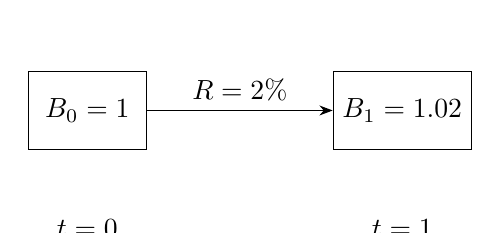
\begin{tikzpicture}[node distance=4cm]
\node[draw, rectangle, minimum width=1.5cm, minimum height=1cm] (B0) {$B_0 = 1$};
\node[draw, rectangle, minimum width=1.5cm, minimum height=1cm, right of=B0] (B1) {$B_1 = 1.02$};
\draw[-{Stealth}] (B0) -- (B1) node[midway, above] {$R = 2\%$};
\node[below of=B0, node distance=1.5cm] {$t = 0$};
\node[below of=B1, node distance=1.5cm] {$t = 1$};
\end{tikzpicture}
\end{center}

\subsubsection{Stock Price}

At time $t = 0$, the stock price is $S_0 = s$. At time $t = 1$, the stock price evolves as
\[
S_1 = \begin{cases}
su & \text{with probability } p_u, \\
sd & \text{with probability } p_d,
\end{cases}
\]
with $0 < d < u$, and $p_u, p_d \in (0,1)$, $p_u + p_d = 1$.

Thus $S_1$ is a random variable defined on $(\Omega, \mathcal{F}, \Prob)$.

Equivalently, we may write
\[
S_1 = sZ,
\]
where
\[
Z = \begin{cases}
u & \text{with probability } p_u, \\
d & \text{with probability } p_d.
\end{cases}
\]

\textbf{Example:}
\begin{center}
\begin{tikzpicture}[node distance=4.5cm]
\node[draw, rectangle, minimum width=1.5cm, minimum height=1cm] (S0) {$S_0 = 100$};
\node[draw, rectangle, minimum width=1.5cm, minimum height=1cm, above right of=S0, node distance=5cm] (S1u) {$S_1 = 120$};
\node[draw, rectangle, minimum width=1.5cm, minimum height=1cm, below right of=S0, node distance=5cm] (S1d) {$S_1 = 80$};
\draw[-{Stealth}] (S0) -- (S1u) node[midway, above] {$p_u = 0.4$};
\draw[-{Stealth}] (S0) -- (S1d) node[midway, below] {$p_d = 0.6$};
\node[below of=S0, node distance=2cm] {$t = 0$};
\node[right of=S1u, node distance=2cm] {$t = 1$};
\end{tikzpicture}
\end{center}

\begin{definition}[Portfolio]
A portfolio is a vector $h = (x,y) \in \R^2$, where $x$ and $y$ denote the absolute quantities of bonds and stocks, respectively. The sign indicates whether the position is long ($> 0$) or short ($< 0$).
\end{definition}

\subsubsection{Assumptions of a Perfect Market}

\begin{itemize}
\item Short sales and fractional holdings are allowed, hence $x, y \in \R$.
\item There is no bid-ask spread.
\item No transaction costs or taxes: the market is frictionless.
\item The market is completely liquid.
\item All agents are price takers and have full information (no insider trading).
\end{itemize}

\subsubsection{Value of a Portfolio}

For $h = (x,y) \in \R^2$, the value process of the portfolio is
\[
V_t^h = xB_t + yS_t.
\]

In particular,
\[
V_0^h = x + ys, \quad V_1^h = x(1 + R) + ysZ.
\]

\begin{definition}[No Arbitrage]
A portfolio $h \in \R^2$ is called an arbitrage portfolio if:
\begin{enumerate}
\item $V_0^h = 0$ (zero initial cost),
\item $\Prob(V_1^h \geq 0) = 1$ (no loss with certainty),
\item $\Prob(V_1^h > 0) > 0$ (positive gain with positive probability).
\end{enumerate}
A situation satisfying the above constitutes a free lunch.
\end{definition}

\newpage
\section{September 16, 2025}

\subsection{No-Arbitrage Condition}

\begin{proposition}
In the one-period binomial model, the no-arbitrage condition holds if and only if
\[
d < 1 + R < u.
\]
\end{proposition}

\begin{proof}
We prove both directions separately.

\textbf{($\Rightarrow$)} Assume no arbitrage holds.

Suppose, by contradiction, that $u \leq 1 + R$. Since $d < u \leq 1 + R$, the stock always underperforms (or equals) the risk-free bond.

Consider the portfolio $h = (x,y) = (s, -1)$, i.e. we short one unit of the stock and invest the proceeds in the risk-free asset.

At time $t = 0$:
\[
V_0^h = xB_0 + yS_0 = s \cdot 1 + (-1) \cdot s = 0.
\]

At time $t = 1$:
\[
V_1^h = xB_1 + yS_1 = s(1 + R) - sZ, \quad Z \in \{u, d\}.
\]

Then
\[
\Prob(V_1^h \geq 0) = \Prob(s(1 + R) - sZ \geq 0) = \Prob(Z \leq 1 + R) = 1,
\]
because both $d$ and $u$ are $\leq 1 + R$.

Moreover,
\[
\Prob(V_1^h > 0) = \Prob(Z < 1 + R) = \begin{cases}
1, & \text{if } u < 1 + R, \\
p_d, & \text{if } u = 1 + R.
\end{cases}
\]

$h$ is an arbitrage portfolio, contradicting the assumption of no arbitrage.

A symmetric argument applies if $d \geq 1 + R$. Hence, necessarily

\begin{center}
\fbox{\parbox{0.6\textwidth}{\centering
\vspace{0.5em}
\textbf{No-Arbitrage Condition:}
\[
d < 1 + R < u
\]
Key inequality: guarantees absence of arbitrage and existence of risk-neutral measure.
\vspace{0.5em}
}}
\end{center}

\textbf{($\Leftarrow$)} Assume $d < 1 + R < u$.

Consider a portfolio $h = (x,y) \in \R^2$ with zero initial value, so that
\[
V_0^h = x + ys = 0 \Rightarrow x = -ys.
\]

Then at time $t = 1$:
\[
V_1^h = x(1 + R) + yS_1 = -ys(1 + R) + ysZ = ys(Z - (1 + R)), \quad Z \in \{u, d\}.
\]

A portfolio $h$ would be an arbitrage if and only if:
\begin{enumerate}[label=(\alph*)]
\item $\Prob(V_1^h \geq 0) = 1$, and
\item $\Prob(V_1^h > 0) > 0$.
\end{enumerate}

Consider condition (a). We require
\[
\Prob(V_1^h \geq 0) = \Prob(ys(Z - (1 + R)) \geq 0).
\]

If $y > 0$, this is equivalent to $\Prob(Z \geq 1 + R)$. But since $d < 1 + R < u$, we have $\Prob(Z \geq 1 + R) = \Prob(Z = u) = p_u \neq 1$.

If $y < 0$, the inequality reverses, so we would need $\Prob(Z \leq 1 + R)$. Again, since $d < 1 + R < u$, we have $\Prob(Z \leq 1 + R) = \Prob(Z = d) = p_d \neq 1$.

Thus condition (a) cannot be satisfied together with (b) in any case. Therefore, no arbitrage portfolio exists, and the no-arbitrage condition holds.
\end{proof}

\begin{remark}
The condition $d < 1 + R < u$ does not depend on the probabilities $p_u, p_d$. This reflects the fact that no-arbitrage is independent of the physical probability measure $\Prob$.
\end{remark}

\subsection{First Fundamental Theorem of Asset Pricing (1FTAP)}

We introduce the model
\[
\pi = (1, s)
\]
as the vector of current prices.

We can define the matrix $D$ of possible future prices (rows represent the assets, columns the states):
\[
D = \begin{bmatrix}
1 + R & 1 + R \\
sd & su
\end{bmatrix}.
\]

\begin{proposition}
No arbitrage holds if and only if there exists a vector
\[
\phi = \begin{bmatrix}
\phi_1 \\
\phi_2
\end{bmatrix}, \quad \phi_1, \phi_2 > 0,
\]
such that
\[
\pi = D\phi.
\]
\end{proposition}

The vector $\phi$ is called the state price vector.
\begin{itemize}
\item $\phi_1$ corresponds to the state $d$,
\item $\phi_2$ corresponds to the state $u$.
\end{itemize}

\textbf{Note:} we have two components $\phi_1, \phi_2$ because there are two possible future states (up and down), not because there are two assets.

We define the normalized weights:
\[
q_d = \frac{\phi_1}{\phi_1 + \phi_2}, \quad q_u = \frac{\phi_2}{\phi_1 + \phi_2},
\]
with $q_i \in (0,1)$.

The solution to the system $\pi = D\phi$ is
\[
\phi = \frac{1}{(1 + R)(u - d)} \begin{bmatrix}
u - (1 + R) \\
(1 + R) - d
\end{bmatrix}.
\]

This implies
\[
q_d = \frac{u - (1 + R)}{u - d}, \quad q_u = \frac{(1 + R) - d}{u - d}.
\]

Since $d < 1 + R < u$, we have $q_d, q_u \in (0,1)$. Hence, $q = (q_d, q_u)$ is a probability vector.

We can therefore define a probability measure $\Q$ on $(\Omega, \mathcal{F})$ such that
\[
\Q(Z = u) = q_u, \quad \Q(Z = d) = q_d.
\]

This is called the risk-neutral probability.

It can be shown that $\Q$ is equivalent to $\Prob$: for all $A \in \mathcal{F}$,
\[
\Prob(A) = 0 \quad \Leftrightarrow \quad \Q(A) = 0,
\]
\[
\Prob(A) = 1 \quad \Leftrightarrow \quad \Q(A) = 1.
\]


We define $\Q$ through the relation $\pi = D\phi$, which is equivalent to the system:
\begin{align}
1 &= (1 + R)\phi_1 + (1 + R)\phi_2 \quad \text{(A)}, \\
s &= sd\phi_1 + su\phi_2 \quad \text{(B)}.
\end{align}

From (A):
\[
1 = (1 + R)(\phi_1 + \phi_2) \quad \Leftrightarrow \quad \phi_1 + \phi_2 = \frac{1}{1 + R},
\]
that is, the sum of the state prices equals the discount factor.

From (B):
\[
s = sd\phi_1 + su\phi_2.
\]

Normalizing by $\phi_1 + \phi_2$:
\[
\frac{s}{\phi_1 + \phi_2} = sdq_d + suq_u,
\]
so that
\[
s = \frac{1}{1 + R}(sdq_d + suq_u) = \E^\Q\left[\frac{1}{1 + R}S_1\right].
\]

Thus we obtain the risk-neutral evaluation formula:

\begin{center}
\fbox{\parbox{0.7\textwidth}{\centering
\vspace{0.5em}
\textbf{Risk-Neutral Valuation Formula:}
\[
s = \E^\Q\left[\frac{1}{1 + R}S_1\right]
\]
}}
\end{center}

\textbf{Comment:}
This formula means that the current value of the stock is equal to the expected discounted future value under the risk-neutral measure $\Q$. In other words, when pricing assets, we can think of the market as if all investors were risk-neutral: the present price is the discounted expectation of the payoff, not under the real-world probabilities $\Prob$, but under $\Q$, which incorporates the absence of arbitrage.

\subsection{Financial Derivatives}

\begin{definition}
A financial derivative (or contingent claim) is a random variable
\[
X = \Phi(Z),
\]
where $\Phi$ is the contract function.
\end{definition}

\textbf{Example.}
An European call option on $S_t$, with maturity $T = 1$ and strike price $K > 0$.

\textbf{Assumption:} $sd < K < su$.
\begin{itemize}
\item If $K > su$, then $S_1 \leq su < K$, so the option is never exercised.
\item If $K < sd$, then $S_1 \geq sd > K$, so the option is always exercised.
\end{itemize}
Hence we assume the non-trivial case $sd < K < su$.

The payoff is
\[
X = \max\{S_1 - K, 0\} = [S_1 - K]^+.
\]

\begin{center}
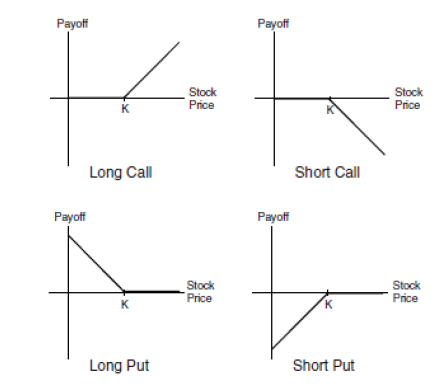
\includegraphics[width=0.8\textwidth]{images/options_payoff.png}
\end{center}

\begin{definition}
The value at time $t$ of a contingent claim $X$ is denoted by $\Pi_t(X)$, for $t = 0, 1$.
\begin{itemize}
\item At maturity: $\Pi_1(X) = X$.
    \item At time 0: $\Pi_0(X) = \E^\Q\left[\frac{1}{1+R}X\right]$ (later we will justify this risk-neutral valuation formula).
\end{itemize}
\end{definition}

\begin{definition}[Replicating Portfolio]
A derivative $X$ is called reachable if there exists a portfolio $h$ such that
\[
V_1^h = X.
\]
In this case, $h$ is called a replicating portfolio.

If all contingent claims are reachable, then the market is said to be complete.
\end{definition}

\textbf{No-Arbitrage Requirement.}
To avoid arbitrage, the price of a derivative must equal the value of its replicating portfolio at all times:
\[
\Pi_t(X) = V_t^h, \quad \forall t.
\]
This is the Law of One Price: two assets with the same payoff must have the same price.

\textbf{Construction.}
The terminal value of a portfolio is
\[
V_1^h = \begin{cases}
x(1 + R) + ysd & \text{if } Z = d, \\
x(1 + R) + ysu & \text{if } Z = u,
\end{cases}
\]
which can be written as
\[
D^T h = \Phi,
\]
where
\[
\Phi = \begin{bmatrix}
\Phi(d) \\
\Phi(u)
\end{bmatrix}.
\]

Thus,
\[
h = (D^T)^{-1}\Phi.
\]
This system has a unique solution since $d < u$, so the matrix is invertible.

Explicitly,
\[
h = \begin{bmatrix}
x \\
y
\end{bmatrix} = \begin{bmatrix}
\frac{1}{1+R} \cdot \frac{u\Phi(d) - d\Phi(u)}{u - d} \\
\frac{1}{s} \cdot \frac{\Phi(u) - \Phi(d)}{u - d}
\end{bmatrix}.
\]

Finally, the value of the derivative at time 0 is given by the initial value of the replicating portfolio:
\[
V_0^h = \Pi_0(X) = x + ys = \E^\Q\left[\frac{1}{1+R}X\right].
\]

\newpage
\section{September 18, 2025}

\subsection{Example 1: European Call Option}

Let the parameters be:
\[
s = 100, \quad u = 1.06, \quad d = 0.98, \quad p_u = 0.6, \quad p_d = 0.4, \quad R = 0.02 \text{ (yearly)}, \quad T = 1 \text{ (year)}.
\]

Define $X$ as a European call option with strike price $K = 104$, i.e.
\[
X = [S_1 - 104]^+.
\]

\textbf{Step 1. Stock Prices}

At $t = 0$:
\[
S_0 = 100.
\]

At $t = 1$:
\[
S_1 = \begin{cases}
106 & \text{with probability } 0.6, \\
98 & \text{with probability } 0.4.
\end{cases}
\]

\textbf{Step 2. Derivative Payoff}

The option payoff at maturity is:
\[
\Phi(u) = 106 - 104 = 2, \quad \Phi(d) = 0.
\]

\textbf{Step 3. Price at $t = 0$}

By the risk-neutral pricing formula:
\[
\Pi_0(X) = \E^\Q\left[\frac{1}{1+R}X\right] = \frac{1}{1.02}(2q_u + 0 \cdot q_d).
\]

Since in this case $q_u = q_d = \frac{1}{2}$,
\[
\Pi_0(X) = \frac{1}{1.02} \cdot \left(2 \cdot \frac{1}{2}\right) = 0.9804.
\]

\textbf{Step 4. Replicating Portfolio}

We use the general formulas (derived from $h = (D^T)^{-1}\Phi$):
\[
x = \frac{1}{1+R} \cdot \frac{u\Phi(d) - d\Phi(u)}{u - d}, \quad y = \frac{1}{s} \cdot \frac{\Phi(u) - \Phi(d)}{u - d}.
\]

Substituting values:
\[
x = \frac{1}{1.02} \cdot \frac{1.06 \cdot 0 - 0.98 \cdot 2}{1.06 - 0.98} = -24.0196, \quad y = \frac{1}{100} \cdot \frac{2 - 0}{1.06 - 0.98} = 0.25.
\]

Thus the replicating portfolio consists of:
\begin{itemize}
\item shorting $24.0196$ units of the bond,
\item buying $0.25$ units of the stock.
\end{itemize}

\textbf{Step 5. Delta Hedging Interpretation}

We can rewrite the replication condition as:
\[
\Pi_t(X) - V_t^h = 0 \quad \Leftrightarrow \quad \Pi_t(X) - (xB_t + yS_t) = 0 \quad \Leftrightarrow \quad \Pi_t(X) - yS_t = xB_t.
\]

\subsection{Example 2: Trinomial Case}

We keep the same data as before, except that now the stock has three possible outcomes at $t = 1$:
\[
Z = \begin{cases}
u = 1.06 & \text{with probability } 0.4, \\
m = 1.00 & \text{with probability } 0.2, \\
d = 0.98 & \text{with probability } 0.4.
\end{cases}
\]

Thus
\[
S_1 = \begin{cases}
106, & p = 0.4, \\
100, & p = 0.2, \\
98, & p = 0.4.
\end{cases}
\]

For the derivative payoff $X$ (European call with strike $K = 104$):
\[
\Phi(u) = 2, \quad \Phi(m) = 0, \quad \Phi(d) = 0.
\]

\textbf{Step 1. Not a Binomial Model}

This is not a binomial model anymore, since the stock has 3 possible outcomes instead of 2.

The equivalent linear algebra description is the following:

Price vector at time $t = 0$:
\[
\pi = (1, 100).
\]

Matrix of possible future prices:
\[
D = \begin{bmatrix}
1.02 & 1.02 & 1.02 \\
98 & 100 & 106
\end{bmatrix}.
\]

\textbf{Step 2. 1FTAP in This Setting}

Recall the First Fundamental Theorem of Asset Pricing (1FTAP):
\[
\text{No Arbitrage holds} \quad \Leftrightarrow \quad \exists \phi = (\phi_1, \phi_2, \phi_3) \in \R^3, \quad \phi_i > 0 \text{ such that } D\phi = \pi.
\]

That is, we must solve a system of two linear equations with three unknowns.

By Rouché-Capelli Theorem:
\begin{itemize}
\item If $\operatorname{rank}(D) \neq \operatorname{rank}(D|\pi)$, no solution exists $\rightarrow$ arbitrage.
\item If $\operatorname{rank}(D) = \operatorname{rank}(D|\pi) = \text{\# unknowns}$, then the solution is unique.
\item If $\operatorname{rank}(D) = \operatorname{rank}(D|\pi) < \text{\# unknowns}$, then there are infinitely many solutions.
\end{itemize}

In our case:
\[
\operatorname{rank}(D) = \operatorname{rank}(D|\pi) = 2.
\]

Since the number of unknowns is 3, the system has infinitely many solutions.

This means there exist multiple risk-neutral measures $\Q$.

\textbf{Step 3. Consequences}

A risk-neutral measure $\Q = (q_u, q_m, q_d)$ exists, but is not unique.

Hence, some contingent claims cannot be replicated uniquely.

In terms of market structure:
\begin{itemize}
\item In the binomial model, completeness follows because the number of states = number of assets.
\item Here, states (3) > assets (2), so the market is incomplete.
\end{itemize}

\textbf{Step 4. Replicating Portfolio Attempt}

We try to replicate the derivative payoff vector:
\[
\Phi = \begin{bmatrix}
\Phi(d) \\
\Phi(m) \\
\Phi(u)
\end{bmatrix} = \begin{bmatrix}
0 \\
0 \\
2
\end{bmatrix}.
\]

We want a portfolio $h = (x,y)$ such that
\[
D^T h = \Phi.
\]

Here
\[
D^T = \begin{bmatrix}
1.02 & 98 \\
1.02 & 100 \\
1.02 & 106
\end{bmatrix}.
\]

Compute ranks:
\[
\operatorname{rank}(D^T) = 2, \quad \operatorname{rank}(D^T|\Phi) = 3.
\]

Thus the system is inconsistent, meaning no solution exists.

\textbf{Conclusion}

There is no replicating strategy for this claim. The market is not complete.

Intuitively, with only 2 traded assets (bond and stock) but 3 possible future states, we do not have enough instruments to span all payoffs. This is the essence of market incompleteness.

Since the claim is not replicable, there does not exist a unique no-arbitrage price (which would correspond to the cost of the replicating portfolio).

Instead, there exists an interval of admissible prices $(\Pi_{\min}, \Pi_{\max})$, generated by taking the check infimum and supremum of the expected discounted payoff:
\[
\Pi_{\min} = \inf_{\Q \in \mathcal{M}} \E^\Q\left[\frac{X}{1+R}\right], \quad \Pi_{\max} = \sup_{\Q \in \mathcal{M}} \E^\Q\left[\frac{X}{1+R}\right],
\]
as $\Q$ varies over all infinitely many possible risk-neutral measures $\mathcal{M}$.

\subsection{Example 3: Three Assets, Binomial Model}

We return to the binomial model, but now the market has three traded assets:
\begin{itemize}
\item the zero-coupon bond (ZCB),
\item stock $S^1$,
\item stock $S^2$.
\end{itemize}

Parameters:
\[
(S_0^1, S_0^2) = (100, 80),
\]
\[
(S_1^1, S_1^2) = \begin{cases}
(106, 83), & p = 0.6, \\
(98, 79), & p = 0.4.
\end{cases}
\]

\textbf{Step 1. Linear Algebra Representation}

Price vector:
\[
\pi = (1, 100, 80).
\]

Matrix of future prices:
\[
D = \begin{bmatrix}
1 & 1 \\
98 & 106 \\
79 & 83
\end{bmatrix}.
\]

We compute:
\[
\operatorname{rank}(D) = \operatorname{rank}(D|\pi) = \text{\# unknowns} = 2.
\]

Hence, there exists a unique risk-neutral measure $\Q$.

\textbf{Step 2. Contingent Claim}

Consider the claim:
\[
X = [S^1 + S^2 - K]^+, \quad K = 185.
\]

At maturity:
\begin{itemize}
\item If $Z = u$: payoff = $106 + 83 - 185 = 4 \rightarrow [4]^+ = 4$.
\item If $Z = d$: payoff = $98 + 79 - 185 = -8 \rightarrow [-8]^+ = 0$.
\end{itemize}

Thus the payoff vector is:
\[
\Phi = \begin{bmatrix}
\Phi(d) \\
\Phi(u)
\end{bmatrix} = \begin{bmatrix}
0 \\
4
\end{bmatrix}.
\]

\textbf{Step 3. Replicating Strategy}

We want $h \in \R^3$ (portfolio weights in bond, $S^1$, $S^2$) such that:
\[
D^T h = \Phi.
\]

Here,
\[
D^T = \begin{bmatrix}
1 & 98 & 79 \\
1 & 106 & 83
\end{bmatrix}.
\]

Ranks:
\[
\operatorname{rank}(D^T) = \operatorname{rank}(D^T|\Phi) = 2 \neq \text{\# unknowns} = 3.
\]

Thus the system is consistent but underdetermined, meaning there are infinitely many replicating strategies.

\textbf{Step 4. Pricing Consequence}

Even if multiple portfolios replicate the same payoff, the initial value of all these portfolios is the same:
\[
\Pi_0(X) = V_0^h.
\]

This follows from the Law of One Price. Hence, the derivative has a unique price, even if the replicating strategy is not unique.

\textbf{Step 5. Summary Scheme}

\begin{center}
\fbox{\parbox{0.9\textwidth}{\centering
\vspace{0.5em}
\textbf{Risk-Neutral Measure:}
\begin{align}
\operatorname{rank}(D) = \operatorname{rank}(D|\pi) &\quad \Rightarrow \quad \exists \Q, \\
\operatorname{rank}(D) = \operatorname{rank}(D|\pi) = \text{\# unknowns} &\quad \Rightarrow \quad \exists! \Q.
\end{align}

\textbf{Replicating Strategy:}
\begin{align}
\operatorname{rank}(D^T) = \operatorname{rank}(D^T|\Phi) &\quad \Rightarrow \quad \exists h, \\
\operatorname{rank}(D^T) = \operatorname{rank}(D^T|\Phi) = \text{\# unknowns} &\quad \Rightarrow \quad \exists! h.
\end{align}
\vspace{0.5em}
}}
\end{center}

\subsection{Generalization of the One-Period Model to Multiple Assets}

\textbf{Setup}

Bond:
\[
B_0 = 1, \quad B_1 = 1 + R.
\]

Stocks:
\[
S_0^1, \ldots, S_0^N \text{ known}, \quad S_1^1, \ldots, S_1^N \text{ random}.
\]

States of the World:
There are $M > 1$ future states.
\[
\Omega = \{\omega_1, \ldots, \omega_M\}, \quad \mathcal{F} = \mathcal{P}(\Omega), \quad \Prob(\{\omega_j\}) = p_j \in (0,1).
\]

\textbf{Random Variables and Contingent Claims}

Any random variable can be represented as a vector
\[
X = (X(\omega_1), \ldots, X(\omega_M))^T \in \R^M.
\]

A contingent claim is exactly such a random variable $X$.

Expectation is given by:
\[
\E[X] = \sum_{j=1}^M X(\omega_j) p_j = X^T p, \quad p = (p_1, \ldots, p_M)^T.
\]

\textbf{Price Matrix}

We define the price matrix $D \in \R^{(N+1) \times M}$:
\[
D = \begin{bmatrix}
1+R & \cdots & 1+R \\
S_1^1(\omega_1) & \cdots & S_1^1(\omega_M) \\
\vdots & \ddots & \vdots \\
S_1^N(\omega_1) & \cdots & S_1^N(\omega_M)
\end{bmatrix}.
\]

\textbf{Portfolios}

\begin{definition}
A portfolio is a vector
\[
h = (h_0, h_1, \ldots, h_N)^T,
\]
where:
\begin{itemize}
\item $h_0$ = number of bonds,
\item $h_i$ = number of units of stock $i$.
\end{itemize}
\end{definition}

\textbf{Value Process of a Portfolio}

The value process is defined as:
\[
V_t^h = h_0 B_t + \sum_{i=1}^N h_i S_t^i = [B_t, S_t^1, \ldots, S_t^N] h.
\]

At time $t = 0$:
\[
V_0^h = h_0 + \sum_{i=1}^N h_i S_0^i = h^T \pi,
\]
which is deterministic, where $\pi = (1, S_0^1, \ldots, S_0^N)$.

At time $t = 1$:
\[
V_1^h(\omega_j) = h_0(1 + R) + \sum_{i=1}^N h_i S_1^i(\omega_j) = [D^T h]_j,
\]
i.e. the $j$-th component of $D^T h$.

\textbf{Arbitrage Definition}

A portfolio $h$ is called an arbitrage portfolio if:
\begin{enumerate}
\item $V_0^h = 0$ (zero initial cost, i.e. $h \perp \pi$),
\item $\Prob(V_1^h \geq 0) = 1$ (non-negativity in all states, i.e. $[D^T h]_j \geq 0$ for all $j$),
\item $\Prob(V_1^h > 0) > 0$ (strict gain in at least one state).
\end{enumerate}

\textbf{First Fundamental Theorem of Asset Pricing (Generalized)}

The 1FTAP holds in this general setting:

No arbitrage $\Leftrightarrow$ there exists a state price vector $\phi \in \R^M$ with strictly positive components such that:
\[
\pi = D\phi, \quad \sum_{j=1}^M \phi_j = \frac{1}{1+R}.
\]

In particular, for each stock $i$:
\[
S_0^i = \frac{1}{1+R} (Dq)_{i+1},
\]
where $q$ is the risk-neutral probability vector.

\newpage
\section{September 22, 2025}

\subsection{The Numéraire Concept}

So far, we have written the risk-neutral valuation formula as
\[
S_0^i = \E^\Q\left[\frac{1}{1+R}S_1^i\right],
\]
where we assumed $B_0 = 1$.

In more general terms, a \textbf{numéraire} is any strictly positive price process $Z_t$ (i.e., $Z_t > 0$ almost surely for all $t$) that serves as a benchmark asset relative to which all other assets are priced.

If we choose $Z_t$ as the numéraire, there exists a probability measure $\Q^Z$ such that the relative price process of any traded asset $S_t$, defined as $\frac{S_t}{Z_t}$, is a martingale under $\Q^Z$.

The choice of the numéraire is mathematically equivalent to a \textbf{change of measure}. When we move from using the risk-free bank account $B$ (yielding the risk-neutral measure $\Q$) to using a stock $S$ (yielding the stock measure $\Q^S$), we are essentially changing the "drift" of the processes so that the new relative ratios become martingales.

\subsection{Market Completeness}

\begin{definition}
The market is called complete if, for every contingent claim $X$, there exists a replicating portfolio $h$ such that
\[
V_1^h = X.
\]
\end{definition}

By the Law of One Price:

At maturity:
\[
\Pi_1(X) = X = V_1^h = D^T h \quad \Leftrightarrow \quad X \in \operatorname{Im}(D^T).
\]

At time 0:
\[
\Pi_0(X) = V_0^h = \pi^T h.
\]

From the risk-neutral valuation formula we know:
\[
\pi = \frac{1}{1+R} Dq.
\]

Plugging this into $\Pi_0(X)$:
\[
\Pi_0(X) = \pi^T h = \frac{1}{1+R}(Dq)^T h = \frac{1}{1+R}q^T(D^T h) = \frac{1}{1+R}q^T X.
\]

Thus,
\[
\Pi_0(X) = \E^\Q\left[\frac{1}{1+R}X\right].
\]

\subsection{Image and Kernel Interpretation}

The condition
\[
X = D^T h \quad \Leftrightarrow \quad X \in \operatorname{Im}(D^T)
\]
means that the claim $X$ belongs to the image of $D^T$, i.e. the set of all vectors that can be reached by linear combinations of the columns of $D^T$.

Recall:
\[
\operatorname{Im}(A) = \{b \in \R^m \mid \exists x \in \R^n, \, Ax = b\}, \quad \ker(A) = \{x \in \R^n \mid Ax = 0\}.
\]

Thus:
\begin{itemize}
\item Completeness means $\operatorname{Im}(D^T) = \R^M$, i.e. every contingent claim can be replicated.
\item Equivalently, this is the same as requiring $\ker(D) = \{0\}$, so that the system $\pi = D\phi$ admits a unique solution.
\item Hence, the risk-neutral measure $\Q$ is unique.
\end{itemize}

\subsection{Second Fundamental Theorem of Asset Pricing (2FTAP)}

We arrive at the key statement:

\begin{center}
\fbox{\parbox{0.7\textwidth}{\centering
\vspace{0.5em}
\textbf{2FTAP:} The market is complete $\Leftrightarrow \exists! \Q$.
\vspace{0.5em}
}}
\end{center}

\subsection{Summary of One-Period Model}

\begin{center}
\fbox{\parbox{0.95\textwidth}{
\vspace{0.5em}

\textbf{Portfolio value:}
For $h = (x,y)$:
\[
V_0^h = x + ys, \quad V_1^h = x(1 + R) + ysZ, \quad Z \in \{u,d\}.
\]

\vspace{0.5em}
\textbf{No-Arbitrage Condition:}
\[
d < 1 + R < u.
\]

\vspace{0.5em}
\textbf{1FTAP (First Fundamental Theorem of Asset Pricing):}
\[
\text{NA} \quad \Leftrightarrow \quad \exists \Q \sim \Prob, \quad \pi = \frac{1}{1+R} Dq,
\]
where $q = (q_d, q_u)$ is the risk-neutral measure.

\vspace{0.5em}
\textbf{Risk-neutral probabilities:}
\[
q_d = \frac{u - (1+R)}{u - d}, \quad q_u = \frac{(1+R) - d}{u - d}.
\]

\vspace{0.5em}
\textbf{Valuation of stock:}
\[
S_0 = \E^\Q\left[\frac{1}{1+R}S_1\right].
\]

\vspace{0.5em}
\textbf{General risk-neutral valuation formula (any claim $X$):}
\[
\Pi_0(X) = \E^\Q\left[\frac{1}{1+R}X\right].
\]

\vspace{0.5em}
\textbf{Replicating portfolio for claim $X$:}
Solve
\[
D^T h = \Phi, \quad \Phi = \begin{bmatrix} \Phi(d) \\ \Phi(u) \end{bmatrix},
\]
yielding:
\[
x = \frac{1}{1+R} \cdot \frac{u\Phi(d) - d\Phi(u)}{u - d}, \quad y = \frac{1}{s} \cdot \frac{\Phi(u) - \Phi(d)}{u - d}.
\]

\vspace{0.5em}
\textbf{Law of One Price:}
\[
\Pi_t(X) = V_t^h, \quad \forall t,
\]
if a replicating portfolio $h$ exists.

\vspace{0.5em}
\textbf{2FTAP (Second Fundamental Theorem of Asset Pricing):}
\[
\text{Market complete} \quad \Leftrightarrow \quad \exists! \Q.
\]
}}
\end{center}


\newpage
\subsection{Multi-Period Binomial Model}

\textbf{Setup}

Probability space:
\[
(\Omega, \mathcal{F}, \Prob), \quad t = 0, 1, \ldots, T, \quad T \in \mathbb{N} \cup \{\infty\}.
\]

Sequence of i.i.d. random variables $(Z_0, Z_1, \ldots, Z_{T-1})$ where
\[
Z_t = \begin{cases}
u & \text{with probability } p_u, \\
d & \text{with probability } p_d,
\end{cases} \quad 0 < d < u.
\]

\textbf{Assets}

Bond (zero-coupon):
\[
B_0 = 1, \quad B_t = (1 + R)^t.
\]

Stock:
\[
S_0 = s, \quad S_t = S_0 \prod_{n=0}^{t-1} Z_n.
\]

\vspace{0.5em}
\begin{center}
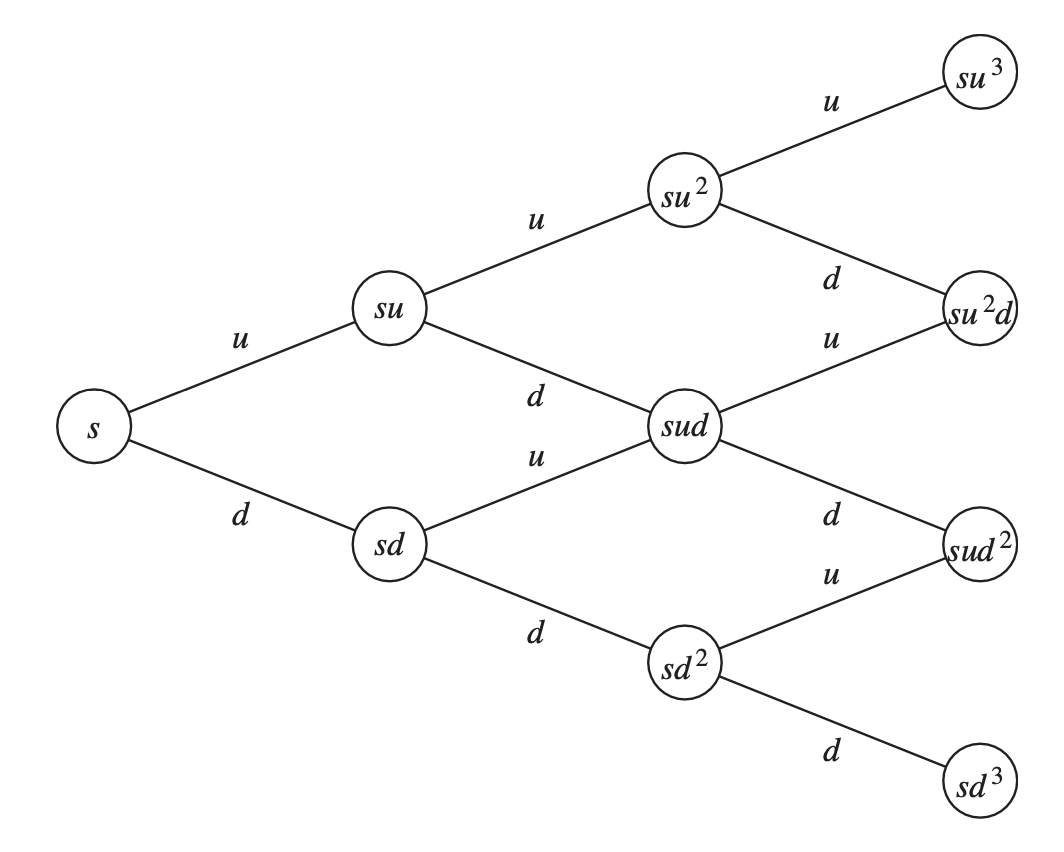
\includegraphics[width=0.8\textwidth]{images/multi_period_model.png}
\end{center}
\vspace{0.5em}

\textbf{Representation with Bernoulli Trials}

Define $Y_0, Y_1, \ldots, Y_{T-1} \sim \text{i.i.d. Bernoulli}(p_u)$, with
\[
Y_t = \begin{cases}
1 & \text{with prob. } p_u \text{ ("up")}, \\
0 & \text{with prob. } p_d \text{ ("down")}.
\end{cases}
\]

Then
\[
\sum_{n=0}^{t-1} Y_n \sim \text{Binomial}(t, p_u),
\]
which counts the number of up moves by time $t$.

Accordingly,
\[
t - \sum_{n=0}^{t-1} Y_n \sim \text{Binomial}(t, p_d),
\]
the number of down moves.

Thus:
\[
S_t = S_0 \prod_{n=0}^{t-1} Z_n = S_0 \, u^{\sum_{n=0}^{t-1} Y_n} d^{t - \sum_{n=0}^{t-1} Y_n}.
\]

\begin{remark}[Connection to Black-Scholes]
If we divide by $S_0$ and take logarithms:
\[
\ln\left(\frac{S_t}{S_0}\right) = \left(\sum_{n=0}^{t-1} Y_n\right) \ln u + \left(t - \sum_{n=0}^{t-1} Y_n\right) \ln d.
\]

This is a sum of i.i.d. random variables.

As $t$ grows, by the Central Limit Theorem, the distribution converges (after normalization) to a Gaussian.

Therefore, in the continuous-time limit, $S_t$ becomes log-normally distributed, which is the core of the Black-Scholes model.
\end{remark}

\textbf{Stochastic Processes}

\begin{definition}
A stochastic process in discrete time is a collection of random variables
\[
X = \{X_t\}_{t=0}^T = (X_0, X_1, \ldots, X_T).
\]

For a fixed $\omega \in \Omega$, the map
\[
t \mapsto X_t(\omega)
\]
is called a path or trajectory of the process $X$.
\end{definition}

\newpage
\section{September 23, 2025}

\subsection{Stochastic Processes and Conditional Expectation}

\textbf{Paths of a Stochastic Process}

Given a stochastic process $X = \{X_t\}_{t=0}^T$ and $\omega \in \Omega$, a path is the map:
\[
t \mapsto X_t(\omega).
\]

\textbf{Example.}
For a binomial model with $t = 2$:
\[
\Omega = \{\omega_{uu}, \omega_{ud}, \omega_{du}, \omega_{dd}\},
\]
with
\[
\mathcal{F} = \mathcal{P}(\Omega), \quad \Prob(\{\omega_{uu}\}) = p_u^2, \quad \Prob(\{\omega_{ud}\}) = \Prob(\{\omega_{du}\}) = p_u p_d, \quad \Prob(\{\omega_{dd}\}) = p_d^2.
\]

For instance, the path corresponding to $\omega_{uu}$ is
\[
S_t(\omega_{uu}) = (S_0, S_1, S_2) = (s, su, su^2).
\]

\textbf{Conditional Probabilities}

Let $B = \{\text{at time 1, the stock made an up move}\}$.

For any event $A \in \mathcal{F}$:
\[
\Prob(A|B) = \frac{\Prob(A \cap B)}{\Prob(B)}.
\]

\textbf{Example.}
Let $A = \{\text{at time 2, the stock made two up moves}\}$. Then:
\[
\Prob_B(A) = \frac{\Prob(A \cap B)}{\Prob(B)} = \frac{p_u^2}{p_u} = p_u.
\]
\[
\Prob_B(A^c) = 1 - \Prob_B(A) = p_d.
\]

\textbf{Conditional Expectation (Intuition)}

Given an event $B = \{S_1 = su\}$ and a r.v. $Y$:
\[
\E[Y|B] = \sum_{\omega \in \Omega} Y(\omega) \Prob_B(\{\omega\}).
\]

\textbf{Example.}
\begin{align}
\E[S_2|S_1 = su] &= S_2(\omega_{uu}) \Prob_B(\{\omega_{uu}\}) + S_2(\omega_{ud}) \Prob_B(\{\omega_{ud}\}) \\
&= su^2 p_u + sud p_d = su(p_u u + p_d d).
\end{align}

Notice:
\[
\E[S_2|S_1 = x] = x(p_u u + p_d d) = f(x).
\]

This shows that conditional expectation can be expressed as a function of the conditioning variable (here $x = S_1$). Since $S_1$ is random, this function evaluated at $S_1$ is again a random variable — so we obtain a stochastic process.

\vspace{0.5em}
\textbf{On $L^1$ and Lipschitz Functions}

We require $Y \in L^1$, i.e. $\E[|Y|] < +\infty$. This ensures that the expected value exists.

A function $f: \R \to \R$ is Lipschitz continuous of order 1 (denoted $f \in \text{Lip}^1$) if there exists a constant $C > 0$ such that
\[
|f(x) - f(y)| \leq C|x - y|, \quad \forall x, y.
\]

More generally, $f \in \text{Lip}^n$ means the same inequality holds with $|x - y|^n$.

\textbf{Intuition.} Lipschitz functions are "controlled continuous functions": they cannot oscillate too wildly, so when applied to random variables, they preserve integrability. In particular, if $f$ is Lipschitz and $X \in L^1$, then $f(X) \in L^1$.


\begin{center}
\vspace{0.5em}
\fbox{\parbox{0.95\textwidth}{
\vspace{0.5em}
\textbf{Key Properties of Conditional Expectation}

For $Y, Z \in L^1$, given a random variable $X$:

\vspace{0.5em}
\begin{enumerate}
\item \textbf{Linearity:}
\[
\E[\alpha Y + \beta Z|X] = \alpha \E[Y|X] + \beta \E[Z|X].
\]

\item \textbf{Monotonicity:} If $0 \leq Y \leq Z$, then
\[
0 \leq \E[Y|X] \leq \E[Z|X].
\]

\item \textbf{Tower Property (Law of Iterated Expectations):}
\[
\E[\E[Y|X]] = \E[Y].
\]

\item \textbf{Measurability:} If $Y$ is $\sigma(X)$-measurable, then
\[
\E[Y|X] = Y \quad \Prob\text{-a.s.}
\]

\item \textbf{Independence:} If $Y \perp X$, then
\[
\E[Y|X] = \E[Y].
\]

\item \textbf{"Take out what you know":} If $Z$ is $\sigma(X)$-measurable,
\[
\E[YZ|X] = Z \cdot \E[Y|X].
\]
\end{enumerate}
}}
\vspace{0.5em}
\end{center}

\vspace{0.5em}
\textbf{Indicator Function Trick}

If $A \in \sigma(X)$ and $Z = 1_A$, then:
\[
\E[Y1_A|X] = 1_A \E[Y|X].
\]

Taking expectations:
\[
\E[Y1_A] = \E[\E[Y|X] 1_A].
\]

\textbf{Comment.}
Here $W = \E[Y|X]$. This property says: "the expected contribution of $Y$ on the event $A$ can be computed equivalently by replacing $Y$ with its conditional expectation $W$". In practice, conditional expectation acts as the "best proxy" for $Y$ when conditioning on the information given by $X$.

\vspace{0.5em}
\textbf{General Definition}

Let $\mathcal{G} \subset \mathcal{F}$ be a sub-$\sigma$-algebra, and $Y \in L^1$. A random variable $Z \in L^1$ is the conditional expectation of $Y$ given $\mathcal{G}$ if:
\begin{enumerate}
\item $Z$ is $\mathcal{G}$-measurable,
\item $\int_A Y \, d\Prob = \int_A Z \, d\Prob, \quad \forall A \in \mathcal{G}$.
\end{enumerate}

Notation:
\[
Z = \E[Y|\mathcal{G}].
\]

\textbf{Comment:} Let $\mathcal{G} \subset \mathcal{F}$ be a sub-$\sigma$-algebra, and $Y \in L^1$. A random variable $Z \in L^1$ is the conditional expectation of $Y$ given $\mathcal{G}$ if:
\begin{enumerate}
\item $Z$ is $\mathcal{G}$-measurable,
\item $\int_A Y \, d\Prob = \int_A Z \, d\Prob, \quad \forall A \in \mathcal{G}$.
\end{enumerate}

\vspace{0.5em}
\textbf{Orthogonality Characterization ($L^2$)}

If $Y \in L^2$:
\[
\E[|Y - \E[Y|\mathcal{G}]|^2] \leq \E[|Y - Z|^2], \quad \forall Z \in L^2, \, Z \text{ } \mathcal{G}\text{-measurable}.
\]

\textbf{Meaning:} The conditional expectation $\E[Y|\mathcal{G}]$ is the best $L^2$-approximation of $Y$ given the information in $\mathcal{G}$.

\subsection{Portfolio Strategy}

\begin{definition}[Portfolio Strategy]
A portfolio strategy is a stochastic process
\[
h = \{h_t\}_{t=1}^T = \{(x_t, y_t)\},
\]
where:
\begin{itemize}
\item $x_t$ = amount invested in the risk-free asset at time $t$,
\item $y_t$ = number of units of the risky asset (stock) held at time $t$.
\end{itemize}
\end{definition}

Thus, $h_t$ is a function of the past stock prices $(S_0, \ldots, S_{t-1})$.

At each time $t$, the investor forms a portfolio $(x_t, y_t)$, keeps it until $t+1$, and then updates. This is the idea of a self-financing strategy.

\subsubsection{Value Process}

The value process of a portfolio $h$ is defined by:
\[
V_t^h = x_t(1 + R) + y_t S_t, \quad t \geq 1,
\]
with
\[
V_0^h = x_0 + y_0 s.
\]

\subsubsection{Remark on Measurability}

We require that each $h_t$ is measurable with respect to the information available up to time $t-1$:
\[
h_t \in \sigma(S_0, \ldots, S_{t-1}).
\]

\textbf{Comment.}
This means that the portfolio choice at time $t$ can only depend on the information already observed up to time $t-1$. In finance: you cannot decide today's allocation based on tomorrow's stock price.

\subsection{Filtration}

\begin{definition}[Filtration]
A filtration is a sequence of sigma-algebras
\[
\mathbb{F} = \{\mathcal{F}_t\}_{t=0}^T,
\]
satisfying:
\begin{enumerate}
\item $\mathcal{F}_t \subseteq \mathcal{F}_t$ for all $t$,
\item If $s \leq t$, then $\mathcal{F}_s \subseteq \mathcal{F}_t$.
\end{enumerate}
\end{definition}

\textbf{Comment.}
A filtration models the flow of information over time. The larger $t$, the more information we have.

\subsubsection{Natural Filtration of a Process}

Given a stochastic process $X = \{X_t\}$, the natural filtration generated by $X$ is
\[
\mathbb{F}^X = \{\mathcal{F}_t^X\}_t, \quad \mathcal{F}_t^X = \sigma(X_s : 0 \leq s \leq t).
\]

This is the minimal filtration that contains all the information carried by the process $X$.

\subsection{Adaptedness and Predictability}

Let $X = \{X_t\}$ be a stochastic process and $\mathcal{F} = \{\mathcal{F}_t\}$ a filtration.

\begin{definition}[Adapted Process]
$X$ is $\mathbb{F}$-adapted if
\[
X_t \text{ is } \mathcal{F}_t\text{-measurable for all } t.
\]
\end{definition}

\textbf{Intuition:} at time $t$, the value of $X_t$ can be determined using the information available at time $t$.

\begin{definition}[Predictable Process]
$X$ is $\mathbb{F}$-predictable if
\[
X_t \text{ is } \mathcal{F}_{t-1}\text{-measurable for all } t.
\]
\end{definition}

\textbf{Intuition:} the decision at time $t$ must be based on information up to time $t-1$.

\begin{remark}[Application to Portfolios]
If $Y$ is $\mathbb{F}^X$-predictable, then
\[
Y_t = g(X_0, \ldots, X_{t-1})
\]
for some measurable function $g$.

Thus, a portfolio strategy $h$ is by definition $\mathbb{F}^S$-predictable, meaning that your trading strategy at time $t$ depends only on the history of the stock up to $t-1$.
\end{remark}

\newpage
\section{September 25, 2025}

\subsection{Portfolio Strategies in Discrete Time}

A portfolio strategy is a stochastic process $h = \{h_t\}_{t=0}^T$ with
\[
h_t = (x_t, y_t),
\]
where $x_t$ is the amount in the risk-free asset and $y_t$ the number of shares of the risky asset. The strategy is $\mathbb{F}$-predictable, i.e.
\[
h_t \text{ is } \mathcal{F}_{t-1}\text{-measurable, hence } h_t = g(S_0, \ldots, S_{t-1}).
\]

\textbf{Comment.} You choose $h_t$ using only information available up to $t-1$.

\subsection{Value Process and Self-Financing}

The value process of $h$ is
\[
V_t^h = x_t B_t + y_t S_t, \quad V_0^h = x_0 + y_0 S_0,
\]
with $B_{t+1} = (1+R)B_t$.

\begin{definition}[Self-Financing Strategy]
The strategy $h$ is self-financing if and only if portfolio value changes only because asset prices move (no external cash flows). Equivalent discrete-time identities:
\begin{equation}
V_{t+1}^h - V_t^h = x_{t+1}(1+R) + y_{t+1}S_{t+1} - x_t(1+R) - y_tS_t = x_tR + y_t(S_{t+1} - S_t)
\end{equation}
\end{definition}

\subsection{Arbitrage (Multi-Period)}

\begin{definition}[Multi-Period Arbitrage]
An arbitrage is a self-financing strategy $h$ such that
\[
V_0^h = 0, \quad \Prob(V_T^h \geq 0) = 1, \quad \Prob(V_T^h > 0) > 0.
\]
\end{definition}

In the binomial model with $d < u$ and risk-free rate $R$, NA holds if and only if
\[
d < 1 + R < u.
\]

\subsection{Martingales and Risk-Neutrality}

Let $(\Omega, \mathcal{F}, \Prob)$ and a filtration $\mathbb{F} = \{\mathcal{F}_t\}$.

\begin{definition}[Martingale]
A process $X = \{X_t\}$ is a $(\Q, \mathcal{F})$-martingale if:
\begin{enumerate}
\item $X$ is $\mathbb{F}$-adapted,
\item $X_t \in L^1$,
\item $\E^\Q[X_{t+1}|\mathcal{F}_t] = X_t$ (equivalently, $\E^\Q[X_t|\mathcal{F}_s] = X_s$ for $s \leq t$).
\end{enumerate}
\end{definition}

\textbf{Interpretation.} Given information $\mathcal{F}_s$, the best prediction of $X_t$ is $X_s$, i.e. $\E^\Q[X_t - X_s|\mathcal{F}_s] = 0$.

\begin{definition}[Equivalent Martingale Measure (EMM)]
A probability $\Q$ on $(\Omega, \mathcal{F})$ is an EMM if:
\begin{enumerate}[label=(\roman*)]
\item $\Q \sim \Prob$ (equivalent), and
\item the discounted price process is a martingale:
\[
\frac{S_t}{B_t} = \E^\Q\left[\frac{S_{t+1}}{B_{t+1}} \mid \mathcal{F}_t\right].
\]
\end{enumerate}
\end{definition}

\textbf{Comment.} Risk-neutral measures are precisely the EMMs.

\begin{theorem}[1FTAP - Multi-Period]
In the binomial model:
\[
\text{NA} \quad \Leftrightarrow \quad \exists \text{ EMM } \Q.
\]
\end{theorem}

From the martingale condition,
\[
S_t = \E^\Q\left[\frac{S_{t+1}}{1+R} \mid \mathcal{F}_t\right] \quad \Rightarrow \quad \frac{S_t}{B_t} = \E^\Q\left[\frac{S_{t+1}}{B_{t+1}} \mid \mathcal{F}_t\right].
\]

In the one-step binomial case this yields
\[
q_u = \frac{(1+R) - d}{u - d}, \quad q_d = 1 - q_u.
\]

\subsection{Contingent Claims and Completeness}

A contingent claim is $X = \Phi(S_T)$ for a Borel $\Phi$.

\begin{theorem}[Law of One Price]
If $X$ is replicable by a self-financing $h$, then
\[
\Pi_t(X) = V_t^h \quad \text{for all } t.
\]
\end{theorem}

In the multi-period binomial model (one stock + bond), under NA the market is complete: every claim is replicable; the EMM is unique.

\subsection{Backward Induction Pricing (Binomial Tree)}

Let $R$ be the per-step risk-free rate and $\Q$ the (unique) EMM with $q_u, q_d$. For a claim $X = \Phi(S_T)$,
\[
\Pi_T = X, \quad \Pi_t =\ ?
\]

\subsection{Worked Example}

\textbf{Parameters:} $T = 3$, $S_0 = 80$, $u = 1.5$, $d = 0.5$, $p_u = 0.6$, $p_d = 0.4$, $R = 0$.

\textbf{NA check:} $d = 0.5 < 1 = 1 + R = 1 < u = 1.5$

\textbf{Risk-neutral probabilities:} with $R = 0$,
\[
q_u u + q_d d = 1 \quad \Rightarrow \quad 1.5 q_u + 0.5(1 - q_u) = 1 \quad \Rightarrow \quad q_u = q_d = \frac{1}{2}.
\]

\textbf{Claim:} $X = [S_T - K]^+$ with $K = 80$.

\textbf{Stock tree:}
\begin{center}
\begin{tabular}{c|c}
$t$ & $S$ \\
\hline
0 & 80 \\
1 & (120, 40) \\
2 & (180, 60, 60, 20) \\
3 & (270, 90, 90, 30, 30, 10) \\
\end{tabular}
\end{center}

\textbf{Payoff at $t = 3$:}
\[
X_T = [S_T - 80]^+: (190, 10, 10, 0, 0, 0).
\]

\textbf{Backward induction} (since $R = 0$, just average under $q = \frac{1}{2}$):

At $t = 2$:
\begin{align}
\Pi_2(180) &= \frac{1}{2}(190 + 10) = 100, \\
\Pi_2(60) &= \frac{1}{2}(10 + 0) = 5 \quad \text{(both middle nodes)}, \\
\Pi_2(20) &= 0.
\end{align}

At $t = 1$:
\begin{align}
\Pi_1(120) &= \frac{1}{2}(100 + 5) = 52.5, \\
\Pi_1(40) &= \frac{1}{2}(5 + 0) = 2.5.
\end{align}

At $t = 0$:
\[
\Pi_0 = \frac{1}{2}(52.5 + 2.5) = 27.5.
\]

\vspace{1.5em}
\begin{center}
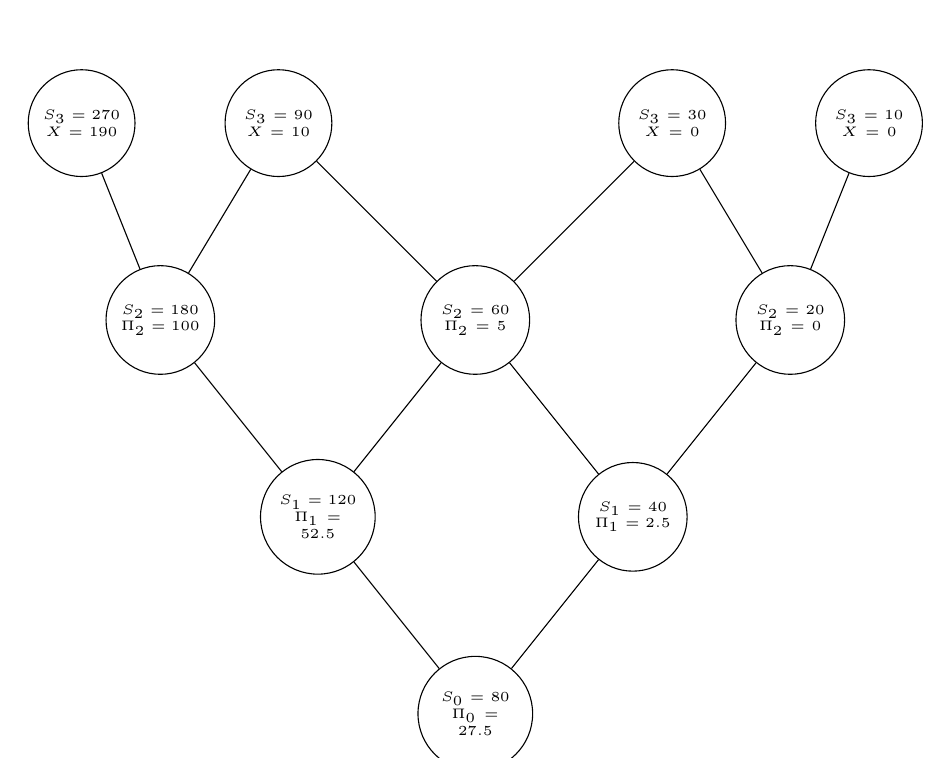
\begin{tikzpicture}[
  every node/.style={circle, draw, minimum size=1.2cm, font=\tiny, text width=1cm, align=center}
]

% t=3
\node (uuu3) at (-5,0) {$S_3 = 270$ \\ $X = 190$};
\node (uud3) at (-2.5,0) {$S_3 = 90$ \\ $X = 10$};
\node (udd3) at (2.5,0) {$S_3 = 30$ \\ $X = 0$};
\node (ddd3) at (5,0) {$S_3 = 10$ \\ $X = 0$};

% t=2
\node (uu2) at (-4,-2.5) {$S_2 = 180$ \\ $\Pi_2 = 100$};
\node (ud2) at (0,-2.5) {$S_2 = 60$ \\ $\Pi_2 = 5$};
\node (dd2) at (4,-2.5) {$S_2 = 20$ \\ $\Pi_2 = 0$};

% t=1
\node (up1) at (-2,-5) {$S_1 = 120$ \\ $\Pi_1 = 52.5$};
\node (down1) at (2,-5) {$S_1 = 40$ \\ $\Pi_1 = 2.5$};

% t=0 (root at bottom)
\node (root) at (0,-7.5) {$S_0 = 80$ \\ $\Pi_0 = 27.5$};

% Connections t=3 to t=2
\draw (uuu3) -- (uu2);
\draw (uud3) -- (uu2);
\draw (uud3) -- (ud2);
\draw (udd3) -- (ud2);
\draw (udd3) -- (dd2);
\draw (ddd3) -- (dd2);

% Connections t=2 to t=1
\draw (uu2) -- (up1);
\draw (ud2) -- (up1);
\draw (ud2) -- (down1);
\draw (dd2) -- (down1);

% Connections t=1 to t=0
\draw (up1) -- (root);
\draw (down1) -- (root);

\end{tikzpicture}
\end{center}

\newpage
\section{September 29, 2025}

\subsection{Multi-Period Binomial Model}

The general formula for the multi-period (discrete, with $T$ steps) model for the price of a derivative with final payoff $\Phi(S_T)$ is:

\begin{center}
\fbox{\parbox{0.8\textwidth}{\centering
\vspace{0.5em}
\textbf{Multi-Period Binomial Pricing Formula:}
\[
\Pi_0 = \sum_{k=0}^T \binom{T}{k} q_u^k q_d^{T-k} \, \Phi\!\left(S_0 u^k d^{T-k}\right)
\]
}}
\end{center}

Where:
\begin{itemize}
\item $\Pi_0$ represents the fair price of the derivative at time 0.
\item $q_u, q_d$ are the risk-neutral probabilities associated with up/down movements.
\item The idea is that the binomial model recreates all possible paths of $S_t$ and calculates the weighted (risk-neutral) average of payoffs.
\end{itemize}

\textit{Intuition: We are "reconstructing" the initial value as the risk-neutral expectation of the final payoff, discounted at the risk-free rate.}

\subsection{Forward Strategy - Replicating Portfolio Construction}

To replicate the derivative, we construct a strategy $h_t = (x_t, y_t)$:
\begin{itemize}
\item $x_t$: amount invested in the risk-free asset
\item $y_t$: number of shares held
\end{itemize}

\subsubsection{Step 1 - Calculation at $t=1$}

Given: $S_0 = 80$, $S_1 = (120, 40)$.
Payoff at time 2: $\Phi_1(u) = 52.5$, $\Phi_1(d) = 2.5$.

Formulas:
\[
x_1 = \frac{1}{1+R} \cdot \frac{u\Phi_1(d) - d\Phi_1(u)}{u-d} = -22.5
\]

\[
y_1 = \frac{1}{S_0} \cdot \frac{\Phi_1(u) - \Phi_1(d)}{u-d} = \frac{5}{8}
\]

Portfolio value:
\[
V_0^h = x_1 + y_1 S_0 = -22.5 + \frac{5}{8} \cdot 80 = 27.5
\]

\textbf{Note:} This coincides with $\Pi_0$, i.e., the correct price of the derivative.

\subsubsection{Step 2 - Calculation at $t=2$}

Node: $S_1 = 120$, future $S_2 = (180, 60)$.
Corresponding payoffs: $\Phi_2(u) = 100$, $\Phi_2(d) = 5$.

Formulas:
\[
x_2 = \frac{1}{1+R} \cdot \frac{u\Phi_2(d) - d\Phi_2(u)}{u-d} = -42.5
\]

\[
y_2 = \frac{\Phi_2(u) - \Phi_2(d)}{S_1(u-d)} = \frac{95}{120}
\]

Strategy cost:
\[
V_1^h = x_2 + y_2 S_1 = 52.5
\]

\textit{Intuition: At each step, the cost of the new portfolio coincides with the derivative value calculated in the previous step - this is the self-financing property.}

\subsection{Binomial Tree - General Structure}

\begin{itemize}
\item Each node is identified by $(t, k)$ with $t$ time and $k$ number of up-moves.
\item Asset price:
\[
S_t = S_0 u^{k_t} d^{t-k_t}
\]
where $k_t \sim \text{Bin}(t, q_u)$.
\item The replicating portfolio is also expressed as a function of $k_t$:
\[
V_t^h = V_t^h(k_t)
\]
\end{itemize}

\subsection{Binomial Algorithm - Backward Recursion}

\textbf{No-arbitrage condition:}
\[
d < 1+R < u
\]

\begin{center}
\fbox{\parbox{0.7\textwidth}{\centering
\vspace{0.5em}
\textbf{Backward Equation:}
\[
V_t^h(k) = \frac{1}{1+R}\Big[q_u V_{t+1}^h(k+1) + q_d V_{t+1}^h(k)\Big]
\]
}}
\end{center}

With terminal condition:
\[
V_T^h(k) = \Phi(S_0 u^k d^{T-k})
\]

\begin{center}
\fbox{\parbox{0.7\textwidth}{\centering
\vspace{0.5em}
\textbf{Forward Strategy:}
\[
h_t(k_{t-1}) = \Big(x_t(k_{t-1}), y_t(k_{t-1})\Big)
\]
}}
\end{center}

\textbf{Intuition:}
\begin{itemize}
\item Backward: calculate derivative values starting from time $T$.
\item Forward: calculate the corresponding replicating strategy.
\end{itemize}

\subsection{Limit of the Binomial Model (→ Black-Scholes)}

\subsubsection{Bond}

Assume $R = r\Delta t$. Then:
\[
B_{t+\Delta t} = B_t(1+r\Delta t)
\]

Taking the limit $\Delta t \to 0$:
\[
\frac{d}{dt}B_t = rB_t, \quad B_0=1 \quad \Rightarrow \quad B_t = e^{rt}
\]

This shows that $r$ is the risk-free rate with continuous compounding.

\subsubsection{Stock}

Model:
\[
S_t = S_0 e^{X_t}, \quad X_t \text{ random variable}
\]

\begin{itemize}
\item $\ln(S_t/S_0) = X_t$ = log-return.
\item Increments:
\[
\ln\!\Big(\frac{S_{t+\Delta t}}{S_t}\Big) = X_{t+\Delta t} - X_t = \xi_n
\]
\end{itemize}

Simple model:
\[
\xi_n =
\begin{cases}
+\Delta X & p=1/2 \\
-\Delta X & p=1/2
\end{cases}, \quad X_0=0
\]

Then:
\[
\ln\!\Big(\frac{S_T}{S_0}\Big) = \sum_{n=0}^{N-1}\xi_n
\]

\textbf{Intuition:} The stock price becomes a discrete Brownian motion that, in the limit $N\to\infty$, leads to the Black-Scholes model.

Properties:
\[
\mathbb{E}[\xi_n] = 0, \quad \text{Var}(\xi_n) = \Delta X^2
\]


\newpage
\section{September 30, 2025}

\subsection{Random Walk and Diffusion Limit}

We start from i.i.d. random variables $\xi_n$ with
\[
\mathbb{E}[\xi_n] = 0, \quad \text{Var}(\xi_n) = \Delta x^2
\]

Therefore, for the random walk $X_n = \sum_{i=1}^n \xi_i$:
\[
\mathbb{E}[X_n] = 0, \quad \text{Var}(X_n) = n \Delta x^2
\]

Since time evolves in discrete steps of size $\Delta t$, we want a diffusion scaling such that:
\[
\lim_{\Delta t \to 0} \frac{\Delta x^2}{\Delta t} = \sigma^2
\]

This ensures that the variance of the limiting process grows linearly in time, which is exactly the key property of Brownian motion.

\subsection{Random Walk with Drift}

We choose:
\[
\Delta x = \sigma \sqrt{\Delta t}
\]

Then the increment can be written as:
\[
X_{n+1} - X_n = \mu \Delta t + \sigma \sqrt{\Delta t}\,\xi_n
\]
where $\xi_n$ is a symmetric $\pm 1$ random variable (a "coin toss").

This is called a random walk with drift:
\begin{itemize}
\item $\mu$ is the deterministic drift.
\item $\sigma$ controls the size of random fluctuations.
\end{itemize}

Properties:
\[
\mathbb{E}[X_{n+1} - X_n] = \mu \Delta t, \quad
\text{Var}(X_{n+1} - X_n) = \sigma^2 \Delta t
\]

\subsection{Stock Price Dynamics in Discrete Time}

We model the stock price as:
\[
S_{n+1} = S_n \, e^{X_n}
\]

with
\[
X_n = \mu \Delta t + \xi_n
\]

Define:
\[
u = e^{\mu \Delta t + \sigma \sqrt{\Delta t}}, \quad
d = e^{\mu \Delta t - \sigma \sqrt{\Delta t}}, \quad
p = \tfrac{1}{2}
\]

This gives that 
\[
\ln\left(\frac{S_n}{S_0}\right) \xrightarrow{D}_{n\to\infty} \mathcal{N}(\mu T, \sigma^2 T)
\]
meaning it converges in law to a normal distribution.

\subsection{Convergence to Normal Distribution}

\begin{proposition}
\[
\frac{X_N - N\mu \Delta t}{\sigma \sqrt{N \Delta t}} \sim \mathcal{N}(0,1)
\]
\end{proposition}

\textbf{Proof idea:} This follows from the Central Limit Theorem, since $X_N$ is the sum of i.i.d. symmetric increments scaled properly.

Therefore:
\[
X_N \sim \mathcal{N}(\mu T, \sigma^2 T), \quad T = N \Delta t
\]

\textbf{Intuition:} In the continuous limit, the random walk with drift converges to a Brownian motion with drift $\mu$ and volatility $\sigma$.

\subsection{Stock in Continuous Time}

In continuous time:
\[
S_t = S_0 e^{X_t}, \quad X_t \sim \mathcal{N}(\mu t, \sigma^2 t)
\]

So,
\[
\frac{S_t}{S_0} = e^{X_t} \sim \text{LogNormal}(\mu t, \sigma^2 t)
\]

\begin{definition}
If $X \sim \mathcal{N}(\mu, \sigma^2)$, then $Y = e^X$ follows a log-normal distribution, denoted:
\[
Y \sim \log\mathcal{N}(\mu, \sigma^2)
\]
\end{definition}

Properties:
\[
\mathbb{E}[Y] = e^{\mu + \frac{1}{2}\sigma^2}, \quad
\text{Var}(Y) = e^{2\mu + \sigma^2}\,(e^{\sigma^2} - 1)
\]


\subsection{Estimation of Parameters from Data}

Given a sequence of observed stock prices $(S_0, S_1, \dots, S_n)$, we compute log-returns:
\[
R_n = \ln\!\left(\frac{S_{n+1}}{S_n}\right) = X_{n+1} - X_n
\]

\textbf{Estimate drift:}
\[
\mathbb{E}[R_n] = \hat{\mu} = \frac{\frac{1}{N} \sum_{n=0}^{N-1} R_n}{\Delta t}
\]

\textbf{Estimate volatility:}
\[
  \Var[R_n] = \hat{\sigma}^2 = \frac{\frac{1}{N-1} \sum_{n=0}^{N-1} (R_n - \bar{R_n})^2}{\Delta t}
\]

\textbf{Intuition:} We use the empirical mean and variance of log-returns to back out $\mu$ and $\sigma$.

\subsection{Risk-neutral measure (Cox–Ross–Rubinstein model)}

Under the risk-neutral measure, the expected growth of $S_t$ is the risk-free rate $r$, not $\mu$.

Risk-neutral probability:
\[
q_u = \frac{e^{r\Delta t} - d}{u - d}, \quad q_d = 1 - q_u
\]

This ensures no-arbitrage in the Cox–Ross–Rubinstein model.

\subsection{Basics of Stochastic Calculus}

We now move from discrete to continuous stochastic processes.

\begin{definition}
A standard Brownian motion $(W_t)_{t \ge 0}$ satisfies:
\begin{enumerate}
\item $W_0 = 0$ a.s.
\item Trajectories are continuous a.s.
\item Increments are independent: $W_t - W_s \perp \!\!\!\perp \mathcal{F}_s$, for $0 \le s < t$
\item Distribution of increments:
\[
W_t - W_s \sim \mathcal{N}(0, t-s)
\]
\end{enumerate}
\end{definition}

\textbf{Important:} Paths are continuous but almost surely nowhere differentiable. This makes integration w.r.t. Brownian motion non-trivial.

\rule{\textwidth}{0.4pt}

\subsection{Itô Integral – Motivation}

We cannot define
\[
\frac{dW_t}{dt}
\]
in the classical sense. Instead, we define integrals of the form:
\[
\int_0^t X_s \, dW_s
\]
where $X$ is an adapted, progressively measurable process.

\rule{\textwidth}{0.4pt}

\subsection{Simple Processes}

A process $\phi_t$ is simple if it is piecewise constant:
\[
\phi_t = \sum_{i=0}^{n-1} g_i \, \mathbf{1}_{[t_i, t_{i+1})}(t)
\]

Then the Itô integral is defined as:
\[
\int_a^b \phi_s \, dW_s = \sum_{i=0}^{n-1} g_i \big(W_{t_{i+1}} - W_{t_i}\big)
\]

We approximate general processes by simple processes and take limits in $L^2$.

\textbf{Intuition:} Think of Itô integrals as limits of Riemann sums, but instead of $\Delta t$ you have increments of Brownian motion $\Delta W_t$.

\newpage
\section{October 6, 2025}

\subsection{Stochastic Integral — Properties and Itô's Formula}

Let $g \in M^2(a,b)$ and consider a natural filtration $\mathbb{F} = \{\mathcal{F}_t\}_{t \geq 0}$.

\subsubsection{Properties}

\textbf{Zero expectation}
\[
\mathbb{E}\left[\int_a^b g_s \, dW_s\right] = 0
\]

\textbf{Intuition:} The Itô integral has mean zero because the Brownian motion has independent increments with zero mean, and the integrand $g_s$ is adapted — it cannot "foresee" future increments.

\textbf{Itô Isometry}
\begin{center}
\fbox{\parbox{0.7\textwidth}{\centering
\[
\mathbb{E}\left[\left(\int_a^b g_s \, dW_s\right)^2\right] = \mathbb{E}\left[\int_a^b g_s^2 \, ds\right]
\]
}}
\end{center}

This is the key identity of Itô calculus. It shows that the stochastic integral preserves the $L^2$-norm up to a deterministic integral — a fundamental link between random and deterministic integration.

\textbf{Adaptedness}

$\int_a^t g_s \, dW_s$ is measurable with respect to $\mathcal{F}_t$.

\textbf{Intuition:} The value of the integral up to time $t$ only depends on the information available up to $t$, not on the future.

\textbf{Martingale Property}

Let $g \in M^2$, then the process
\[
I_t = \int_0^t g_s \, dW_s, \quad t \in [0,T]
\]
is $\mathbb{F}$-adapted and is a martingale.

\textbf{Intuition:} The expected future value equals the present one — stochastic integrals are the canonical examples of continuous-time martingales.

\textbf{Gaussianity}

If $g \in L^2$ and $g$ is deterministic, then:
\[
I_t = \int_0^t g(s) \, dW_s \sim \mathcal{N}\left(0, \int_0^t g(s)^2 \, ds\right)
\]

If $g$ were random, this would no longer hold exactly — conditional on the path of $g$, it remains Gaussian but with random variance.

\subsection{Itô's Formula}

Let $X = \{X_t\}_{t \geq 0}$ be a stochastic process.

We say that $X$ admits a stochastic differential if there exist processes $\mu_t \in \mathbb{R}$ and $\sigma_t \in M^2$ such that, almost surely,
\[
X_t = X_0 + \int_0^t \mu_s \, ds + \int_0^t \sigma_s \, dW_s, \quad \forall t \geq 0
\]

In differential form:
\[
dX_t = \mu_t \, dt + \sigma_t \, dW_t, \quad X_0 \text{ given}.
\]

Here:
\begin{itemize}
\item $\mu_t$ is the drift process,
\item $\sigma_t$ is the diffusion (volatility) process.
\end{itemize}

\subsubsection{Expectation and Variance}

Using Fubini–Tonelli theorem, that allows us to interchange the expectation and the deterministic integral: $\mathbb{E}\left[\int_0^t \mu_s \, ds\right] = \int_0^t \mathbb{E}[\mu_s] \, ds$. We can "move the expectation inside" the integral when integrating with respect to deterministic time $ds$.
\[
\mathbb{E}[X_t] = X_0 + \mathbb{E}\left[\int_0^t \mu_s \, ds\right] + \mathbb{E}\left[\int_0^t \sigma_s \, dW_s\right] = X_0 + \int_0^t \mathbb{E}[\mu_s] \, ds
\]

Note that $\mathbb{E}\left[\int_0^t \sigma_s \, dW_s\right] = 0$ by Property 1 above (zero expectation).



We can thus write informally:
\[
\frac{d}{dt}\mathbb{E}[X_t] = \mathbb{E}[\mu_t]
\]

Hence, $\mathbb{E}[\mu_t]$ represents the instantaneous average rate of change of $X_t$. That's why $\mu_t$ is often called the drift, since it describes the average evolution of the process.

For the variance:
\[
\text{Var}(X_t) = \mathbb{E}\left[\int_0^t \sigma_s^2 \, ds\right]
\]

and informally:
\[
\frac{d}{dt}\text{Var}(X_t) = \mathbb{E}[\sigma_t^2]
\]

which defines $\mathbb{E}[\sigma_t^2]$ as the instantaneous volatility of the process.

\subsubsection{Computing the Stochastic Differential of a Function}

We now want to compute the differential of a transformed process
\[
Z_t = f(t, X_t)
\]
where $f: [0,T] \times \mathbb{R} \to \mathbb{R}$ is twice continuously differentiable.

\textbf{Heuristic Derivation}

We start from a first-order Taylor expansion:
\[
\Delta Z_t = f(t + \Delta t, X_{t+\Delta t}) - f(t, X_t)
\]

Approximate $X_{t+\Delta t} = X_t + \mu_t \Delta t + \sigma_t \Delta W_t$.

Then:
\[
\Delta Z_t \approx f_t(t, X_t) \Delta t + f_x(t, X_t) \Delta X_t
\]

but since $\Delta X_t = \mu_t \Delta t + \sigma_t \Delta W_t$,
\[
\Delta Z_t \approx f_t \Delta t + f_x(\mu_t \Delta t + \sigma_t \Delta W_t)
\]

\textbf{Intuition:} So far we are only using the deterministic chain rule. However, because $\Delta W_t$ has variance of order $\Delta t$, second-order terms cannot be ignored.

The crucial observation is that:
\[
(\Delta W_t)^2 \approx \Delta t, \quad \text{as } \Delta t \to 0
\]

\textbf{Explanation:} The variance of $(\Delta W_t)^2$ is:
\[
\text{Var}((\Delta W_t)^2) = \mathbb{E}[(\Delta W_t)^4] - (\mathbb{E}[(\Delta W_t)^2])^2 = 3(\Delta t)^2 - (\Delta t)^2 = 2(\Delta t)^2
\]

Since $\text{Var}((\Delta W_t)^2) = 2(\Delta t)^2 \to 0$ faster than $\Delta t \to 0$, by the law of large numbers, $(\Delta W_t)^2$ converges in probability to its expectation $\Delta t$:
\[
(\Delta W_t)^2 \xrightarrow{P} \Delta t \quad \text{as } \Delta t \to 0
\]

while higher-order moments vanish:
\[
\mathbb{E}[(\Delta W_t)^3] = 0, \quad \mathbb{E}[(\Delta W_t)^4] = 3(\Delta t)^2
\]

Hence, to properly capture the stochastic behavior, we need a second-order Taylor expansion.

\textbf{Second-Order Correction}

Including second-order terms:
\[
\Delta Z_t \simeq f_t \Delta t + f_x \Delta X_t + \frac{1}{2} f_{xx} (\Delta X_t)^2
\]

Substitute $\Delta X_t = \mu_t \Delta t + \sigma_t \Delta W_t$:
\[
(\Delta X_t)^2 = \mu_t^2 (\Delta t)^2 + 2\mu_t \sigma_t \Delta t \Delta W_t + \sigma_t^2 (\Delta W_t)^2
\]

Since $(\Delta W_t)^2 \approx \Delta t$ and other terms are of higher order, we get:
\[
(\Delta X_t)^2 \approx \sigma_t^2 \Delta t
\]

Thus:
\[
\Delta Z_t \approx f_t \Delta t + f_x(\mu_t \Delta t + \sigma_t \Delta W_t) + \frac{1}{2} f_{xx} \sigma_t^2 \Delta t
\]

\textbf{Final Differential Form (Itô's Lemma)}

In differential notation:
\begin{center}
\fbox{\parbox{0.9\textwidth}{\centering
\[
dZ_t = df(t, X_t) = \left(f_t + \mu_t f_x + \frac{1}{2} \sigma_t^2 f_{xx}\right) dt + \sigma_t f_x \, dW_t
\]
}}
\end{center}

The additional term $\frac{1}{2} \sigma_t^2 f_{xx} \, dt$ is the "Itô correction," accounting for the curvature of $f$ with respect to $X_t$ and the randomness of Brownian motion.

\subsection{Examples}

\textbf{Example 1 — $Z_t = W_t^4$}

\textbf{Computing $dZ_t$ using Itô's formula:}

$Z_t = f(t, X_t) = W_t^4 \implies f(t, x) = x^4$, where $X_t = W_t$ ($dX_t = dW_t$ with $\mu_t = 0, \sigma_t = 1$).

Computing the partial derivatives:
\begin{align}
f_t &= \frac{\partial f}{\partial t} = 0 \quad \text{(no explicit time dependence)} \\
f_x &= \frac{\partial f}{\partial x} = 4x^3 \quad \Rightarrow \quad f_x(W_t) = 4W_t^3 \\
f_{xx} &= \frac{\partial^2 f}{\partial x^2} = 12x^2 \quad \Rightarrow \quad f_{xx}(W_t) = 12W_t^2
\end{align}

Applying Itô's formula: $dZ_t = \left(f_t + \mu_t f_x + \frac{1}{2} \sigma_t^2 f_{xx}\right) dt + \sigma_t f_x \, dW_t$
\[
dZ_t = \left(0 + 0 \cdot 4W_t^3 + \frac{1}{2} \cdot 1^2 \cdot 12W_t^2\right) dt + 1 \cdot 4W_t^3 \, dW_t
\]
\[
dZ_t = 6W_t^2 \, dt + 4W_t^3 \, dW_t
\]

\textbf{Computing $\mathbb{E}[W_t^4]$ using Itô's formula:}

From the differential $dZ_t = 6W_s^2 \, ds + 4W_s^3 \, dW_s$, integrating from $0$ to $t$, and since $Z_t = W_t^4$ and $Z_0 = W_0^4 = 0$:
\[
W_t^4 = \int_0^t 6W_s^2 \, ds + \int_0^t 4W_s^3 \, dW_s
\]
\[
Z_t = W_t^4 = W_0^4 + \int_0^t 6W_s^2 \, ds + \int_0^t 4W_s^3 \, dW_s
\]

Taking expectations and using the zero expectation property of stochastic integrals:
\[
\mathbb{E}[W_t^4] = \mathbb{E}\left[\int_0^t 6W_s^2 \, ds\right] + \mathbb{E}\left[\int_0^t 4W_s^3 \, dW_s\right] = \int_0^t 6\mathbb{E}[W_s^2] \, ds + 0
\]

Since $\mathbb{E}[W_s^2] = s$:
\[
\mathbb{E}[W_t^4] = \int_0^t 6s \, ds = 3t^2
\]

\textbf{Example 2 — Geometric Brownian Motion}

Let
\[
dX_t = \mu X_t \, dt + \sigma X_t \, dW_t, \quad X_0 \in \mathbb{R}_+
\]

Define $S_t = e^{X_t}$. Then by Itô's lemma:
\[
dS_t = S_t\left(\left(\mu + \frac{1}{2}\sigma^2\right) dt + \sigma \, dW_t\right)
\]

Thus, $S_t$ follows a geometric Brownian motion (GBM).

\newpage
\section{October 7, 2025}

\subsection{Stochastic Differential Equations (SDEs)}

\begin{center}
\fbox{\parbox{0.92\textwidth}{\centering
\vspace{0.3em}
\textbf{Definition (SDE).} A stochastic differential equation is an identity of the form
\[
 dX_t = \alpha(t, X_t)\, dt + \sigma(t, X_t)\, dW_t, \qquad X_0 \in \R,
\]
where $(W_t)_{t\ge 0}$ is a standard Brownian motion on a filtered probability space $(\Omega,\mathcal{F},(\mathcal{F}_t)_{t\ge 0},\Prob)$.

\vspace{0.3em}
\textbf{Integral formulation.} A process $X = \{X_t\}_{t\ge 0}$ is a solution if, for every $t\ge 0$,
\[
 X_t = X_0 + \int_0^t \alpha(s, X_s)\, ds + \int_0^t \sigma(s, X_s)\, dW_s, \qquad \Prob\text{-a.s.}
\]
\vspace{0.3em}
}}
\end{center}

Here $\alpha:[0,\infty)\times \R\to\R$ and $\sigma:[0,\infty)\times \R\to\R$ are measurable (drift and diffusion), and $(W_t)$ is $(\mathcal{F}_t)$-adapted.

\subsubsection*{Assumptions}
We assume:
\begin{itemize}
  \item \textbf{Adaptedness:} $\alpha(t,x)$ and $\sigma(t,x)$ are progressively measurable.
  \item \textbf{Integrability:} for all $t\ge 0$,
  \[
    \int_0^t \big(|\alpha(s,0)|^2 + |\sigma(s,0)|^2\big) ds < \infty, \quad \text{a.s.}
  \]
  \item \textbf{Lipschitz continuity (A\textsubscript{1}):} there exists $L>0$ such that
  \[
    |\alpha(t,x)-\alpha(t,y)| + |\sigma(t,x)-\sigma(t,y)| \le L|x-y|, \quad \forall\, x,y\in\R,\; t\ge 0.
  \]
  \item \textbf{Linear growth (A\textsubscript{2}):} there exists $M>0$ such that
  \[
    |\alpha(t,x)| + |\sigma(t,x)| \le M(1+|x|), \quad \forall\, x\in\R,\; t\ge 0.
  \]
\end{itemize}

\begin{theorem}[Existence and Uniqueness]
Under (A\textsubscript{1}) and (A\textsubscript{2}), the SDE admits a unique strong (pathwise) solution $X = \{X_t\}_{t\ge 0}$ in $M^2$ (the space of square-integrable adapted processes).
\end{theorem}

\begin{remark}[Markov Property]
Solutions to such SDEs are Markov processes: for $0\le s<t$ and all $A\in\mathcal{B}(\R)$,
\[
 \Prob\big(X_t\in A\mid \mathcal{F}_s\big) = \Prob\big(X_t\in A\mid X_s\big),
\]
equivalently, for any bounded measurable $f$,
\[
 E\big[f(X_t)\mid \mathcal{F}_s\big] = E\big[f(X_t)\mid X_s\big].
\]
\end{remark}

\subsection{Portfolio Dynamics in Continuous Time}

\textbf{Market setup.} Finite horizon $T>0$, $N$ assets $S^1,\dots,S^N$, frictionless trading, continuous rebalancing. Let
\[
 h_t = (h_t^1,\dots,h_t^N), \qquad S_t=(S_t^1,\dots,S_t^N), \qquad V_t^h = \sum_{i=1}^N h_t^i S_t^i.
\]

\subsubsection*{Discrete-time intuition}
At time $t$ choose $h_t$. At $t+\Delta t$,
\[
 V_{t+\Delta t}^h = \sum_{i=1}^N h_t^i S_{t+\Delta t}^i.
\]
Rebalancing from $h_t$ to $h_{t+\Delta t}$ costs $\sum_i (h_{t+\Delta t}^i-h_t^i) S_{t+\Delta t}^i$.

\subsubsection*{Self-financing condition}
No external cash flows implies the budget constraint $\sum_i h_t^i S_t^i = V_t^h$ for all $t$. Formally,
\[
 V_{t+\Delta t}^h - V_t^h = \sum_i h_t^i\,(S_{t+\Delta t}^i-S_t^i) + \sum_i (h_{t+\Delta t}^i-h_t^i) S_{t+\Delta t}^i.
\]
Adding and subtracting $\sum_i (h_{t+\Delta t}^i-h_t^i) S_t^i$ we obtain in the limit
\[
 dV_t^h = \sum_{i=1}^N h_t^i\, dS_t^i.
\]
Define the relative weights $u_t^i = \dfrac{h_t^i S_t^i}{V_t^h}$ so that $\sum_i u_t^i = 1$. Then equivalently
\[
 \frac{dV_t^h}{V_t^h} = \sum_{i=1}^N u_t^i\, \frac{dS_t^i}{S_t^i}.
\]

\begin{center}
\begin{tabular}{p{0.45\textwidth} p{0.45\textwidth}}
\centering \( dV_t^h = \sum\limits_{i=1}^N h_t^i\, dS_t^i \) & \centering \( \dfrac{dV_t^h}{V_t^h} = \sum\limits_{i=1}^N u_t^i\, \dfrac{dS_t^i}{S_t^i} \) \\
\end{tabular}
\end{center}

\subsection{The (Generalized) Black--Scholes Model}

We consider one bond $B_t$ and one stock $S_t$.

\subsubsection*{Bond}
\[
 dB_t = r_t B_t\, dt, \qquad B_0>0,
\]
where $(r_t)$ is $\mathcal{F}_t$-adapted. The instantaneous return is $\dfrac{1}{B_t}\dfrac{dB_t}{dt}=r_t$. If $r_t\equiv r$ is constant, then $B_t = e^{rt}$.

\subsubsection*{Stock}
\[
 dS_t = S_t\big[\,\alpha(t,S_t)\, dt + \sigma(t,S_t)\, dW_t\,\big], \qquad S_0>0,
\]
with instantaneous return $\dfrac{1}{S_t} dS_t = \alpha(t,S_t)\, dt + \sigma(t,S_t)\, dW_t$.

\subsubsection*{Discount factor}
For time-varying $r_t$, define $v_t = e^{-\int_0^t r_s ds}$. Then $B_t v_t = B_0$ is constant, so $v_t$ is the stochastic discount factor.

\subsubsection*{Classical Black--Scholes--Merton (BSM)}
\[
 \begin{cases}
 dB_t = r B_t\, dt, & r>0, \\
 dS_t = S_t(\alpha\, dt + \sigma\, dW_t), & \alpha\in\R,\; \sigma>0.
 \end{cases}
\]
\textbf{Risk-neutral interpretation.} Under an equivalent martingale measure, replacing $\alpha$ by $r$ makes the discounted price $e^{-rt} S_t$ a martingale, ensuring no-arbitrage.

\newpage
\section{October 9, 2025}

\subsection{Contingent Claims and Examples}

\begin{definition}[Contingent Claim]
A contingent claim with maturity $T>0$ is any random variable $X:\Omega\to\R$ which is $\mathcal{F}_T$-measurable. Here, $S=(S_t)_{t\in[0,T]}$ denotes the price process of the underlying asset.
\end{definition}

\subsubsection*{Simple Contingent Claims}
A contingent claim is said to be \emph{simple} if
\[
X = \Phi(S_T)
\]
for some measurable function $\Phi:\R\to\R$.

\textbf{Intuition.} A simple claim depends only on the terminal value $S_T$ (e.g. standard European options). Non-simple claims may depend on the entire path $(S_t)_{t\in[0,T]}$.

\subsubsection*{Types of Options}

\paragraph{American Call/Put Options} An American option can be exercised at any time $t\in[0,T]$. In contrast, European options can only be exercised at maturity $T$.

\paragraph{Forward / Futures Contracts} A forward contract is an agreement between two parties: agent $A$ agrees to buy from $B$ a given amount of the underlying asset at time $T$ for a fixed price $K$ (the forward price). The price at time $t=0$ is usually zero (no initial cost). The payoff at maturity is
\[
X = \Phi(S_T) = S_T - K.
\]
\textbf{Intuition.} The forward buyer gains if the market price $S_T$ exceeds the agreed price $K$, and loses otherwise.

\paragraph{Asian Options} An Asian option has the same contractual structure as a European option, but the strike or the underlying price is replaced with the average price of $S_t$ over $[0,T]$. Fixed-strike example:
\[
X = \Bigg[\frac{1}{T}\int_0^T S_t\,dt - K\Bigg]^+.
\]
\textbf{Note.} This $X$ is not simple because it depends on the whole path of $S_t$, however it is still $\mathcal{F}_T$-measurable.

\paragraph{Lookback Options} A lookback option has the same structure as a European option, but the price or strike is replaced by the maximum or minimum value of $S_t$ over $[0,T]$. Lookback call example:
\[
X = S_T - \inf_{0\le t\le T} S_t.
\]
\textbf{Intuition.} Lookback options let the holder ``look back'' over the history of $S_t$ and exercise based on the best (or worst) price achieved during the period.

\subsubsection*{Option Moneyness}
At a given time $t$:
\begin{itemize}[leftmargin=*]
  \item \textbf{In the Money (ITM):} Immediate exercise is profitable $\Rightarrow$ intrinsic value $>0$.
  \item \textbf{Out of the Money (OTM):} Exercise is not profitable.
  \item \textbf{At the Money (ATM):} Indifferent between exercising or not.
\end{itemize}

\subsubsection*{Pricing a Contingent Claim}
Let $\Pi_t(X)$ denote the price of the contingent claim $X$ at time $t\in[0,T]$. \\
By the Law of One Price, we must have $\Pi_T(X)=X$.

If there are no arbitrage opportunities, the market can be represented by the triplet $(B_t,S_t,\Pi_t(X))$, where $B_t$ is the price of the risk-free asset (the num\`eraire). \\
We therefore expect the process $(\Pi_t(X))_{t\in[0,T]}$ to be consistent and determined by the dynamics of $S_t$.

\subsection{Black--Scholes Equation}

\subsubsection*{Assumptions}
We assume that the derivative is traded in the market (not over the counter), that the No-Arbitrage (NA) condition holds, and that the price of the derivative can be written as
\[
\Pi_t(X) = F(t, S_t)
\]
where $F \in C^{1,2}([0,T] \times \R)$, i.e. $F$ is once continuously differentiable in $t$ and twice in $S$.

\subsubsection*{Notation}
For functions $g, h: [0,T] \times \R \to \R$, we use the shorthand $g, h$, and denote their partial derivatives by $g_t, g_s, g_{ss}$, etc.

\subsubsection*{Idea of the Derivation}
\begin{enumerate}
\item Invest in the derivative and in the stock: Consider a long position in one unit of the derivative, and a short position of $\Delta$ shares of the underlying stock.
\item Form a locally riskless portfolio.
\item Compare it with the bond, which is locally riskless as well.
\item Find the equation satisfied by $F$.
\end{enumerate}

\subsubsection*{Step 1: Value of the Portfolio}
The value of the hedged portfolio is
\[
V_t^h = \Pi_t(X) - \Delta S_t = F - \Delta S_t.
\]

Since the portfolio is self-financing, we have
\[
dV_t^h = dF - \Delta \, dS_t.
\]

Applying Itô's lemma to $F(t, S_t)$:
\[
dF = \left(F_t + \alpha S_t F_s + \frac{1}{2}\sigma^2 S_t^2 F_{ss}\right) dt + \sigma S_t F_s \, dW_t.
\]

Substitute into $dV_t^h$:
\begin{align}
dV_t^h &= \left(F_t + \alpha S_t F_s + \frac{1}{2}\sigma^2 S_t^2 F_{ss}\right) dt + \sigma S_t F_s \, dW_t \\
&\quad - \Delta S_t (\alpha \, dt + \sigma \, dW_t).
\end{align}

Simplifying:
\[
dV_t^h = \left(F_t + \alpha S_t F_s + \frac{1}{2}\sigma^2 S_t^2 F_{ss} - \Delta \alpha S_t\right) dt + \sigma S_t (F_s - \Delta) \, dW_t.
\]

\subsubsection*{Step 2: Eliminate the Stochastic Term}
To make the portfolio locally riskless, we eliminate the stochastic part by choosing
\[
\Delta = F_s.
\]

Hence, the $dW_t$ term vanishes and we obtain:
\[
dV_t^h = \left(F_t + \frac{1}{2}\sigma^2 S_t^2 F_{ss}\right) dt.
\]

\subsubsection*{Step 3: Apply the No-Arbitrage Condition}
By the no-arbitrage principle, the instantaneous rate of return of this riskless portfolio must coincide with the risk-free rate $r$.

Therefore:
\[
\frac{1}{V_t^h} \frac{dV_t^h}{dt} = \frac{1}{V_t^h} \left(F_t + \frac{1}{2}\sigma^2 S_t^2 F_{ss}\right) = r.
\]

This implies:
\[
F_t + \frac{1}{2}\sigma^2 S_t^2 F_{ss} = r V_t^h = r F - r \Delta S_t.
\]

Substituting $\Delta = F_s$:
\[
F_t + \frac{1}{2}\sigma^2 S_t^2 F_{ss} - r F + r S_t F_s = 0.
\]

\subsubsection*{Step 4: The Black--Scholes Partial Differential Equation}
We finally obtain the backward PDE:

\begin{center}
\fbox{\parbox{0.8\textwidth}{\centering
\vspace{0.5em}
\textbf{Black--Scholes PDE:}
\[
\begin{cases}
F_t + \frac{1}{2}\sigma^2 S_t^2 F_{ss} + r S_t F_s - r F = 0, \\
F(T, s) = \Phi(s),
\end{cases}
\]
where $\Phi(s)$ is the payoff of the derivative at maturity.
\vspace{0.5em}
}}
\end{center}

\newpage
\section{October 13, 2025}

\subsection{Black--Scholes PDE}

We recall the \textbf{Black--Scholes pricing equation} for a derivative with price $F(t,s)$, where $t \le T$ and $s>0$:

\begin{center}
\fbox{\parbox{0.82\textwidth}{\centering
\vspace{0.5em}
\[
\begin{cases}
F_t + r s F_s + \dfrac{1}{2}\,\sigma^2 s^2 F_{ss} - r F = 0, \\
F(T,s) = \Phi(s).
\end{cases}
\]
\vspace{0.25em}
\textit{Backward parabolic PDE with terminal condition at $t=T$.}
\vspace{0.5em}
}}
\end{center}

\textbf{Why backward parabolic?} Time runs \emph{backwards} from $T$ to $0$ because the terminal payoff is prescribed at $t=T$ and we solve for earlier times. The equation is \emph{parabolic} since the only second-order term is $F_{ss}$, typical of diffusion.

To fully determine the solution, we also need \emph{boundary conditions} describing $F(t,s)$ as $s\to 0^+$ and $s\to +\infty$.

\begin{remark}[Why $\alpha$ does not appear]
The real-world drift $\alpha$ (the stock's local mean return) does not appear because pricing is carried out under a \emph{risk-neutral measure}. In a risk-neutral world, every tradable asset grows on average at the risk-free rate $r$, and the hedging argument eliminates exposure to $\alpha$. Hence the PDE contains $r$ but not $\alpha$.
\end{remark}

\subsection{Solving the Black--Scholes PDE -- Sketch}

Assume constants $\alpha,\sigma,r$. We transform the PDE to the \textbf{heat equation}.

\subsubsection*{Reminder: Heat Equation (standard form)}

\begin{center}
\fbox{\parbox{0.8\textwidth}{\centering
\vspace{0.25em}
\[
\mathsf{H}:\quad \begin{cases}
u_t - D\,u_{xx} = 0, \\
u(0,x) = U_0(x),
\end{cases}\qquad D>0.
\]
\vspace{0.25em}
}}
\end{center}

\textbf{Fundamental solution (heat kernel).} For $\Gamma_D(t,x) = \dfrac{1}{\sqrt{4\pi D t}}\exp\!\left(-\dfrac{x^2}{4Dt}\right)$, if $U_0$ is suitably regular (e.g. continuous with linear growth), then
\[
u(t,x) = \int_{\R} U_0(y)\, \Gamma_D(t, x-y)\,dy.
\]
For $D = \sigma^2/2$, this becomes
\[
u(t,x) = \int_{\R} U_0(y)\, \exp\!\left(-\frac{(x-y)^2}{2\sigma^2 t}\right) dy \cdot \frac{1}{\sqrt{2\pi \sigma^2 t}}.
\]

\textbf{Probabilistic form.} If $X_t^x = x + \sigma W_t$, then $X_t^x\sim\mathcal{N}(x,\sigma^2 t)$ and
\[
u(t,x) = \E\big[ U_0(X_t^x) \big].
\]

\subsection{Applying to Option Pricing}

Consider a European Call payoff $\Phi(S)=[S-K]^+$, $K>0$. Perform the change of variables
\[
x = \ln\!\left(\frac{S}{K}\right),\qquad \tau = \frac{\sigma^2}{2}(T-t),\qquad v(\tau,x) = \frac{1}{K}\, F\!\left(Ke^{x},\, T - \frac{2}{\sigma^2}\,\tau\right).
\]
Intuition: $x$ turns multiplicative moves in $S$ into additive moves; $\tau$ reverses and rescales time; $v$ normalizes price.

With $k = \dfrac{2r}{\sigma^2}$, the PDE becomes
\[
\begin{cases}
v_\tau = v_{xx} + (k-1)v_x - k v, \\
v(0,x) = (e^x - 1)^+.
\end{cases}
\]

\textbf{Eliminate first-/zero-order terms.} Define
\[
\alpha = \frac{k-1}{2},\qquad \beta = -\frac{(k+1)^2}{4},\qquad u(\tau,x) = e^{-(\alpha x + \beta \tau)}\, v(\tau,x).
\]
Then $u$ solves the \emph{standard heat equation}
\[
u_\tau = u_{xx},\qquad u(0,x) = \big(e^{\frac{k+1}{2}x} - e^{\frac{k-1}{2}x}\big)^+.
\]
Hence $u$ is given via the heat kernel or, equivalently, probabilistically; transforming back yields $v$ and then $F$.

\subsection{Final closed-form solution}

The transformed solution is
\[
v(\tau,x) = e^{x} N(d_1) - e^{-k\tau} N(d_2),
\]
with
\[
d_1 = \frac{x + (k+1)\tau}{\sqrt{2\tau}} = \frac{\ln(S/K) + \big(r + \tfrac{1}{2}\sigma^2\big)(T-t)}{\sigma\sqrt{T-t}},\qquad d_2 = d_1 - \sqrt{2\tau} = d_1 - \sigma\sqrt{T-t}.
\]

\paragraph{Return to original variables.} We obtain the \textbf{Black--Scholes formula} for a European Call and Put:

\begin{center}
\fbox{\parbox{0.82\textwidth}{\centering
\vspace{0.25em}
\[
\boxed{\; C_{\BS}(t,s) = s\,N(d_1) - K e^{-r(T-t)} N(d_2) \;}
\]
\vspace{0.25em}
\[
\boxed{\; P_{\BS}(t,s) = K e^{-r(T-t)} N(-d_2) - s\,N(-d_1) \;}
\]
\vspace{0.25em}
where $\displaystyle d_1 = \frac{\ln(s/K) + (r + \tfrac{1}{2}\sigma^2)(T-t)}{\sigma\sqrt{T-t}},\; d_2 = d_1 - \sigma\sqrt{T-t}$.
\vspace{0.25em}
}}
\end{center}

\paragraph{Put--Call Parity.} Since $N(-d_1)=1-N(d_1)$, we have
\begin{center}
\fbox{\parbox{0.5\textwidth}{\centering
\[ C_{\BS}(t,s) - P_{\BS}(t,s) = s - K e^{-r(T-t)}. \]
}}
\end{center}

\newpage
\section{October 16, 2025}

\subsection{Risk-Neutral Valuation Framework}

We start with the general dynamics of the money market account and the risky asset.

\subsubsection{Generalized Black-Scholes Model}

\begin{center}
\fbox{\parbox{0.9\textwidth}{\centering
\vspace{0.5em}
\textbf{Risk-neutral valuation formula:}
\[
\begin{cases}
dB_t = r(t) B_t \, dt, & B_0 \in \R, \; r(t) \text{ deterministic}, \\
dS_t = S_t(\alpha(t, S_t) \, dt + \sigma(t, S_t) \, dW_t), & S_0 \in \R, \; \alpha, \sigma \text{ deterministic}.
\end{cases}
\]
\vspace{0.5em}
}}
\end{center}

This represents the generalized Black–Scholes model with time- (or state-) dependent drift and volatility.

From the classical Black–Scholes result, we know that:
\[
C_{BS}(t, s) = s \, N(d_1(t, s)) - K e^{-r(T-t)} N(d_2(t, s)).
\]

In particular, at time $t = 0$ with $S_0 = s > 0$,
\[
C_{BS}(0, s) = s \, N(d_1) - K e^{-rT} N(d_2).
\]

We expect that the option price should satisfy the risk-neutral pricing formula:
\[
C_{BS}(0, s) = \E^\Q[e^{-rT}[S_T - K]^+], \quad \text{with } \Q \sim \Prob.
\]

\subsubsection{Why Not Use the Physical Measure?}

\textbf{Why can't we directly use the physical probability measure $\Prob$?}

Because under $\Prob$, the drift of $S_t$ is given by the physical rate of return $\alpha(t, S_t)$, not the risk-free rate $r(t)$.

Therefore, the discounted asset price is not a martingale under $\Prob$, and the usual expectation formula does not hold.

\subsubsection{Attempt: Logarithmic Transformation}

We try to write $S_t = s \, e^{X_t}$, where
\[
X_t \sim N\left(\left(r - \frac{1}{2}\sigma^2\right)t, \, \sigma^2 t\right).
\]

Recall that for a contingent claim $X = \Phi(S_T)$, the arbitrage-free price is $\Pi_t(X) = F(t, S_t)$, where $F \in C^{1,2}$ solves the Black–Scholes PDE:
\[
\begin{cases}
F_t + r s F_s + \frac{1}{2}\sigma^2 s^2 F_{ss} - r F = 0, \\
F(T, s) = \Phi(s).
\end{cases}
\]

\subsubsection{General Structure of the Pricing PDE}

More generally, the pricing PDE can be written as:
\[
\begin{cases}
F_t + \mu F_s + \frac{1}{2}\gamma^2 F_{ss} - r F = 0, \\
F(T, x) = \Phi(x).
\end{cases}
\]

In our case:
\[
\mu = r x, \quad \gamma = \sigma x \quad \text{with } x = s.
\]

\subsubsection{Feynman–Kac Representation}

Under the assumptions of the Feynman–Kac theorem, the solution is:
\[
F(t, x) = E\left[\exp\left(-\int_t^T r(s) \, ds\right)\Phi(X_T^{t,x})\right],
\]
where $X_u^{t,x}$ denotes the process starting at $x$ at time $t$, and satisfying the SDE:
\[
\begin{cases}
dX_u = \mu(u, X_u) \, du + \gamma(u, X_u) \, dW_u, \\
X_t = x.
\end{cases}
\]

In the Black–Scholes framework, this becomes:
\[
\begin{cases}
dX_u = r X_u \, du + \sigma X_u \, dW_u, \\
X_t = x.
\end{cases}
\]

However, we notice a problem: These are not the dynamics of $S_t$ under the physical measure $\Prob$, because under $\Prob$ the drift is $\alpha$, not $r$.

\subsubsection{Goal: Find a Risk-Neutral Measure}

\textbf{Goal:} Find a measure $\Q \sim \Prob$ under which $S$ has risk-neutral dynamics.

We want:
\[
\begin{cases}
dS_u = S_u(r \, du + \sigma \, dW_u^Q), \\
S_t = s,
\end{cases}
\]
where $W^\Q$ is a Brownian motion under the new measure $\Q$.

If such a measure $\Q$ exists, then by Feynman–Kac:
\[
F(t, S_t) = \E^\Q\left[\exp\left(-\int_t^T r(s) \, ds\right)\Phi(S_T^{t,s}) \mid \mathcal{F}_t\right].
\]

Because $S$ is a Markov process, conditioning on $\mathcal{F}_t$ is equivalent to conditioning on the current value $S_t$:
\[
F(t, S_t) = \E^\Q\left[\exp\left(-\int_t^T r(s) \, ds\right)\Phi(S_T^{t,s}) \mid S_t\right].
\]

Hence the price of the claim is:
\[
\Pi_t(X) = F(t, S_t) = \E^\Q\left[\exp\left(-\int_t^T r(s) \, ds\right)\Phi(S_T) \mid \mathcal{F}_t\right].
\]

\subsubsection{How to Find the Risk-Neutral Measure}

\textbf{How do we find such a measure $\Q$?}

We compare the dynamics under the physical measure $\Prob$ and the desired dynamics under $\Q$:

\textbf{Under $\Prob$:}
\[
dS_t = S_t(\alpha(t, S_t) \, dt + \sigma(t, S_t) \, dW_t).
\]

\textbf{Under $\Q$:}
\[
dS_t = S_t(r(t) \, dt + \sigma(t, S_t) \, dW_t^\Q).
\]

To transform one into the other, define:
\[
W_t^\Q = W_t - \int_0^t \frac{r(u) - \alpha(u, S_u)}{\sigma(u, S_u)} \, du.
\]

Then:
\[
dW_t^\Q = dW_t - \frac{r(t) - \alpha(t, S_t)}{\sigma(t, S_t)} \, dt.
\]

Substituting this into the $\Prob$-dynamics:
\begin{align}
dS_t &= S_t\left[\alpha(t, S_t) \, dt + \sigma(t, S_t)\left(dW_t^\Q + \frac{r(t) - \alpha(t, S_t)}{\sigma(t, S_t)} \, dt\right)\right] \\
&= S_t(r(t) \, dt + \sigma(t, S_t) \, dW_t^\Q).
\end{align}

Thus, we obtain the desired risk-neutral dynamics.

But is $W_t^\Q$ really a Brownian motion under some measure $\Q$?

To justify this, we need a change of measure theorem.

\subsection{Girsanov's Theorem}

\begin{theorem}[Girsanov's Theorem]
Let $W$ be a Wiener process on $(\Omega, \mathcal{F}, \Prob, \mathbb{F})$, and let $T > 0$ be a fixed time horizon.

Let $\phi = (\phi_t)_{t \in [0,T]}$ be a process in $M^2(0,T)$ and define, for $t \in [0,T]$:
\[
L_t = \exp\left(\int_0^t \phi_s \, dW_s - \frac{1}{2}\int_0^t \phi_s^2 \, ds\right).
\]

Assume that $(L_t)$ is a positive martingale.

Define a new probability measure $\Q$ by:
\[
\Q(A) = \E^\Prob[L_T \mathbf{1}_A], \quad A \in \mathcal{F}_T.
\]

Then $\Q \sim \Prob$, and the process
\[
W_t^\Q = W_t - \int_0^t \phi_s \, ds
\]
is a Brownian motion under $\Q$.
\end{theorem}

\subsection{Remarks on the Girsanov Density}

By Itô's formula, the process $L_t$ defined by
\[
dL_t = L_t \, \phi_t \, dW_t, \quad L_0 = 1,
\]
solves the SDE above.

By analogy with the ODE
\[
\frac{df}{dt} = \phi(t) f(t), \quad f(0) = 1,
\]
we call $L_t$ the \textbf{stochastic exponential} of the process
\[
I_t = \int_0^t \phi_s \, dW_s.
\]

Furthermore, since $L_t$ is a martingale and $L_0 = 1$, we have
\[
\E[L_t] = 1.
\]

\subsection{Application to the Black–Scholes Model}

In the Black–Scholes framework, we apply Girsanov's theorem using
\[
\phi_t = \frac{r(t) - \alpha(t, S_t)}{\sigma(t, S_t)}.
\]

Assuming appropriate conditions on $r, \alpha, \sigma$, this guarantees the existence of a probability measure $\Q \sim \Prob$ under which the discounted price becomes a martingale and $S$ satisfies the risk-neutral dynamics.

\begin{definition}[Risk-Neutral Measure]
A probability measure $\Q$ on $(\Omega, \mathcal{F})$ is called \textbf{risk-neutral} if:
\begin{enumerate}
\item $\Q \sim \Prob$ (equivalent measures),
\item Under $\Q$, the asset price satisfies
\[
dS_t = S_t(r(t) \, dt + \sigma(t, S_t) \, dW_t^\Q).
\]
\end{enumerate}
\end{definition}

\subsection{Combining the Black–Scholes PDE with Feynman–Kac}

From the Black–Scholes PDE and the Feynman–Kac representation, we obtain the \textbf{Risk-Neutral Valuation Formula}.

Let $X = \Phi(S_T)$ be a simple contingent claim.

Then the no-arbitrage price in the B\&S model is:
\[
\Pi_t(X) = F(t, S_t) = \E^\Q\left[\exp\left(-\int_t^T r(u) \, du\right)\Phi(S_T^{t,s})\right].
\]

\subsubsection{Remarks}

\begin{itemize}
\item $\Pi_t$ inherits linearity from the expectation under $\Q$.
\item The process $S^{t,s}$ is the solution of the SDE:
\[
\begin{cases}
dS_u = S_u(r(u) \, du + \sigma(u, S_u) \, dW_u^\Q), & u \in [t, T], \\
S_t = s.
\end{cases}
\]
\end{itemize}

Thus, we can rewrite the pricing formula as:
\[
F(t, s) = \E^\Q\left[e^{-\int_t^T r(u) \, du}\Phi(S_T) \mid S_t = s\right] = \E_{t,s}^\Q\left[e^{-\int_t^T r(u) \, du}\Phi(S_T)\right].
\]
Both notations are equivalent.

\subsubsection{Economic Interpretation}

We are computing the expected present value of the payoff under the risk-neutral measure $\Q$.

This is a mathematical tool, not an economic statement: we do not live in a risk-neutral world.

If the world were truly risk-neutral, the local rate of return of the stock would equal the risk-free rate $r$, which is not generally true under the physical measure $\Prob$.

\subsection{Fundamental Property}

\begin{proposition}
In the Black–Scholes model, for every traded asset, its price process $\Pi_t$ satisfies that the discounted price
\[
Z_t = \frac{\Pi_t}{B_t}
\]
is a martingale under $\Q$.
\end{proposition}

This mirrors the discrete-time theory: absence of arbitrage implies the existence of an equivalent martingale measure under which discounted prices are martingales.

\subsection{Example: Pricing a European Call Option}

We compute the probability that the option finishes in the money, i.e. $S_T^{t,s} \geq K$.

Using the risk-neutral dynamics, we have:
\[
S_T^{t,s} = s \exp\left(\left(r - \frac{1}{2}\sigma^2\right)(T-t) + \sigma(W_T^Q - W_t^Q)\right).
\]

Taking logarithms:
\[
\ln\left(\frac{S_T^{t,s}}{K}\right) = \ln\left(\frac{s}{K}\right) + \left(r - \frac{1}{2}\sigma^2\right)(T-t) + \sigma(W_T^Q - W_t^Q).
\]

Since $W_T^\Q - W_t^\Q \sim \sqrt{T-t} \, Z^\Q$ with $Z^\Q \sim \mathcal{N}(0,1)$, we get:
\[
S_T^{t,s} \geq K \quad \Longleftrightarrow \quad Z^\Q \geq - \frac{\ln(s/K) + (r - \frac{1}{2}\sigma^2)(T-t)}{\sigma\sqrt{T-t}} = - d_2.
\]

Thus:
\[
\mathbf{1}_{\{S_T \geq K\}} = \mathbf{1}_{\{Z^\Q \geq -d_2\}}
\]

\newpage
\section{October 20, 2025}

\subsection{Forward Contracts}

Let $X = \Phi(S_T)$ be a contingent claim whose payoff depends on the underlying price $S_T$ at maturity $T$.

\begin{definition}[Forward Contract]
A forward contract is an agreement between two parties, $A$ and $B$, on the delivery of the contingent claim $X$ at time $T$, with the following structure:
\begin{itemize}
\item Party $A$ (the holder) will pay a fixed amount $K$ at time $T$.
\item Party $B$ (the receiver) will deliver the contingent claim $X$ in exchange for $K$.
\end{itemize}
At the contract initiation time $t$, no cash is exchanged. Therefore, the spot price (current contract value) of entering the forward at time $t$ is:
\[
\text{Spot price at } t = 0.
\]
\end{definition}

Our goal is to determine the forward price:
\[
f(t; T, X) = K,
\]
where:
\begin{itemize}
\item $t$: time of entering the contract,
\item $T$: delivery date,
\item $X$: contingent claim to be delivered,
\item $K$: delivery price agreed at time $t$.
\end{itemize}

\subsubsection{Payoff at Maturity}

At time $T$, the net payoff of the forward contract is:
\[
Y := X - K.
\]

Thus, a forward contract is itself a contingent claim, with payoff $Y$.

\subsubsection{Risk-Neutral Valuation}

By definition of forward contracts, the value of entering the contract at time $t$ is zero:
\[
\Pi_t(Y) = \Pi_t(X - K) = 0.
\]

Since pricing operator $\Pi$ is linear, we obtain:
\[
\Pi_t(X) = \Pi_t(K).
\]

Now recall the risk-neutral valuation formula:
\[
\Pi_t(X) = e^{-r(T-t)} \E_{t,S}^\Q[X],
\]
and since $K$ is deterministic,
\[
\Pi_t(K) = e^{-r(T-t)} K.
\]

Hence,
\[
e^{-r(T-t)} \E_{t,S}^\Q[X] = e^{-r(T-t)} K \quad \Longrightarrow \quad K = f(t; T, X) = \E_{t,S}^\Q[X].
\]

\begin{center}
\fbox{\parbox{0.8\textwidth}{\centering
\vspace{0.5em}
\textbf{Forward Price Formula:}
\[
f(t; T, X) = \E_{t,S}^\Q[X]
\]
The forward price is the risk-neutral expectation of the payoff.
\vspace{0.5em}
}}
\end{center}

\subsubsection{Example: $X = S_T$}

Consider the special case where the contingent claim is simply the underlying:
\[
X = S_T.
\]

Then
\[
f(t; T, X) = \E_{t,S}^\Q[S_T].
\]

Under the risk-neutral measure $\Q$, the stock follows:
\[
S_T = S_t \exp\left\{\left(r - \frac{1}{2}\sigma^2\right)(T-t) + \sigma(W_T^Q - W_t^Q)\right\}.
\]

Thus,
\[
\E^\Q[S_T \mid S_t] = S_t \, \E^\Q\left[\exp\left\{\left(r - \frac{1}{2}\sigma^2\right)(T-t) + \sigma(W_T^\Q - W_t^\Q)\right\}\right].
\]

Factor out constants:
\[
= S_t \exp\left\{\left(r - \frac{1}{2}\sigma^2\right)(T-t)\right\} \cdot \E^\Q\left[\exp\left\{\sigma(W_T^\Q - W_t^\Q)\right\}\right].
\]

Now, $W_T^\Q - W_t^\Q \sim \mathcal{N}(0, T-t)$.

For a normally distributed variable $Z \sim \mathcal{N}(0, \tau)$,
\[
\E[e^{\sigma Z}] = e^{\frac{1}{2}\sigma^2 \tau}.
\]

Applying this:
\[
\E^\Q\left[\exp\left\{\sigma(W_T^\Q - W_t^\Q)\right\}\right] = \exp\left\{\frac{1}{2}\sigma^2(T-t)\right\}.
\]

Therefore,
\[
\E^\Q[S_T \mid S_t] = S_t \exp\left\{\left(r - \frac{1}{2}\sigma^2\right)(T-t) + \frac{1}{2}\sigma^2(T-t)\right\} = S_t e^{r(T-t)}.
\]

Hence,
\[
f(t; T) = f(t; T, S_T) = S_t e^{r(T-t)}.
\]

\begin{center}
\fbox{\parbox{0.7\textwidth}{\centering
\vspace{0.5em}
\textbf{Forward Price for Stock:}
\[
f(t; T) = S_t e^{r(T-t)}
\]
}}
\end{center}

\subsubsection{Intuition}

From
\[
S_t \E^\Q\left[\exp\left(\left(r - \frac{1}{2}\sigma^2\right)(T-t) + \sigma(W_T^\Q - W_t^\Q)\right)\right]
\]
we split deterministic and stochastic parts. The Brownian increment has zero mean, but we are taking expectation of an exponential of a Gaussian variable. The moment generating function compensates exactly the $-\frac{1}{2}\sigma^2$ term, leaving only $e^{r(T-t)}$.

Thus, the randomness disappears in expectation, and only the risk-free growth rate $r$ remains.

\begin{remark}
Even though the spot price of the forward at time $t$ is zero, the spot price at any intermediate time $s \in (t, T)$ can be different from zero.

That is, the value of the forward contract evolves over time, but the forward price $f(t; T, X) = K$ is fixed at inception.

Therefore, the spot price and the forward price are not the same object.
\end{remark}

\subsection{Futures}

A futures contract is similar to a forward: it requires the delivery of a security at time $T$ in exchange for the futures price.

\textbf{Key difference:}
The value of entering a futures contract is always 0 at any time, not just at inception.

\textbf{Why?} Because of marking to market.

\subsubsection{Marking to Market}

Suppose the futures price today is 100.

You enter a long futures contract with a margin account, depositing some collateral.

If tomorrow the futures price rises to 120:
\begin{itemize}
\item The long gains $+20$, which is credited to their margin account.
\item The short loses $-20$, which is debited from their margin account.
\end{itemize}

As a result, the contract is rebalanced daily, and its value is reset to zero each day.

Therefore, the entry cost is always zero at any time, not just at initial time $t$.

This continuous adjustment ensures that the current value of the futures position is always zero, which is the defining difference from forwards.

\subsubsection{Why the Delivery Price Is Not Paid at Maturity}

Because of this daily revaluation and settlement, the contract is effectively reset to zero value at the end of each trading day. After each mark-to-market adjustment:
\begin{itemize}
\item the new futures price becomes the new reference point,
\item past gains/losses have already been realized.
\end{itemize}

Hence, by the final maturity date, the entire profit or loss has already been fully settled through the margin account.

Therefore, there is no need to actually pay the original delivery price (e.g. 100): the contract has been "unwound" day by day.

So, the delivery price is not a future payment obligation, but rather an initial fair value reference used only to compute daily variations.

\subsubsection{Why Use Futures Instead of Buying the Underlying?}

Futures are not just a simplified version of the underlying asset.

In practice, they are often a superior instrument, especially for professional traders.

They provide major advantages:
\begin{itemize}
\item \textbf{Leverage:} you only post a margin, not the full notional value.
\item No need to finance the asset purchase.
\item No custody or storage issues.
\item Short selling is immediate and unrestricted.
\item Very high liquidity and tight bid-ask spreads.
\item Low transaction costs.
\item No long-term counterparty risk: the clearing house guarantees performance.
\item Access to assets or indices that cannot be physically bought.
\item Often more favorable tax treatment.
\end{itemize}

Therefore, futures are not a substitute only when the underlying is unavailable; in many cases, they are strictly more efficient and powerful than trading the underlying directly.

\begin{remark}
If the interest rate $r$ is deterministic, then the pricing of forwards and futures coincides:
\[
F(t; T, X) = f(t; T, X) = \E_{t,S}^\Q[X].
\]
This happens because, under deterministic interest rates, the timing of cash flows from marking-to-market does not create additional value compared to receiving the payoff at maturity.
\end{remark}

\subsection{Options on Futures}

Consider a futures contract on an underlying asset $S$, i.e. a future with payoff $X = S_{T_1}$ and futures price $F(t; T_1)$.

Now we introduce a call option with maturity $T < T_1$, written on this futures contract.

At time $T$, the holder of the option:
\begin{itemize}
\item Receives a long position on the future with maturity $T_1$ $\Rightarrow$ The entry price of a future is always 0 (mark-to-market).
\item Receives the stochastic payoff
\[
X = [F(T; T_1) - K]^+,
\]
where $K$ is the strike of the option.
\end{itemize}

Thus, the option payoff depends on the futures price at time $T$ for delivery at $T_1$.

\subsubsection{Valuation under the Risk-Neutral Measure}

To price the call at time $t$, we compute
\[
\Pi_t(X) = \E_{t,S}^\Q[e^{-r(T-t)} X].
\]

By risk-neutral pricing of futures:
\[
F(T; T_1) = f(T; T_1) = \E^\Q[S_{T_1} \mid \mathcal{F}_T] = S_T e^{r(T_1 - T)}.
\]

Substituting:
\[
X = [S_T e^{r(T_1 - T)} - K]^+ = e^{r(T_1 - T)} [S_T - e^{-r(T_1 - T)} K]^+.
\]

So the payoff is simply a scaled call on $S_T$, with strike $e^{-r(T_1 - T)} K$, multiplied by the factor $e^{r(T_1 - T)}$.

Define:
\[
Y := S_T - e^{-r(T_1 - T)} K.
\]

Then:
\[
X = e^{r(T_1 - T)} Y^+.
\]

\subsubsection{Risk-Neutral Pricing}

\[
\Pi_t(X) = \E_{t,S}^\Q[e^{-r(T-t)} e^{r(T_1 - T)} Y^+] = e^{-r(T_1 - t)} \, \E_{t,S}^\Q[Y^+].
\]

But $Y^+ = [S_T - K']^+$ with $K' = e^{-r(T_1 - T)} K$.

Therefore, $\E_{t,S}^\Q[Y^+]$ is precisely the price of a Black–Scholes call option on $S$ with:
\begin{itemize}
\item maturity $T$,
\item strike $K' = e^{-r(T_1 - T)} K$.
\end{itemize}

Hence:
\[
\Pi_t(X) = e^{r(T_1 - T)} \, C_{BS}(t, s; T, e^{-r(T_1 - T)} K).
\]

Using the standard Black–Scholes formula,
\[
C_{BS}(t, s; T, K') = s \, N(d_1) - e^{-r(T-t)} K' N(d_2),
\]
we get:
\[
\Pi_t(X) = e^{r(T_1 - T)} [s N(d_1) - e^{-r(T-t)} e^{-r(T_1 - T)} K N(d_2)].
\]

Here:
\[
d_1 = \frac{1}{\sigma\sqrt{T-t}} \left[\ln\left(\frac{s}{e^{-r(T_1 - T)} K}\right) + \left(r + \frac{1}{2}\sigma^2\right)(T-t)\right], \quad d_2 = d_1 - \sigma\sqrt{T-t}.
\]

\subsubsection{Expressing the Formula in Terms of the Futures Price}

Note that
\[
F(t; T_1) = s \, e^{r(T_1 - T)}.
\]

Thus:
\[
s = F(t; T_1) \, e^{-r(T_1 - T)}.
\]

Substituting into the formula yields the Black-76 formula for a call on a future:

\begin{center}
\fbox{\parbox{0.8\textwidth}{\centering
\vspace{0.5em}
\textbf{Black-76 Formula for Call on Future:}
\[
C_{BS}^f(t) = e^{-r(T-t)} [F \, N(d_1) - K \, N(d_2)]
\]
with
\[
d_1 = \frac{1}{\sigma\sqrt{T-t}} \left[\ln\left(\frac{F}{K}\right) + \frac{1}{2}\sigma^2(T-t)\right], \quad d_2 = d_1 - \sigma\sqrt{T-t}
\]
where $F = F(t; T_1)$ is the current futures price.
\vspace{0.5em}
}}
\end{center}

This is the standard Black-76 model, widely used in practice for pricing options on futures.

\subsection{Discretization of the Black–Scholes Model and Volatility Estimation}

Consider the time interval $[0, T]$ and discretize it as:
\[
\{0, \Delta t, 2\Delta t, \ldots, N\Delta t = T\}.
\]

Define the log-returns:
\[
R_n = \ln\left(\frac{S_{t_{n+1}}}{S_{t_n}}\right).
\]

From the continuous-time GBM solution:
\[
R_n \stackrel{\mathcal D}{=} \alpha \Delta t + \sigma \sqrt{\Delta t} \, Z_n, \quad Z_n \stackrel{\text{i.i.d.}}{\sim} \mathcal{N}(0,1).
\]

Thus, we can reconstruct the price process:
\[
S_{t_{n+1}} = S_{t_n} e^{R_n}, \quad S_{t_0} = S_0.
\]

\subsubsection{Approximation of Increments}

Define:
\[
\Delta S_{t_n} = S_{t_{n+1}} - S_{t_n} = S_{t_n} (e^{R_n} - 1).
\]

For small $\Delta t$,
\[
e^{R_n} - 1 \approx R_n, \quad \Rightarrow \quad \Delta S_{t_n} \approx S_{t_n} R_n = S_{t_n} (\alpha \Delta t + \sigma \sqrt{\Delta t} Z_n).
\]

Compare this with the SDE of a GBM:
\[
dS_t = S_t (\alpha \, dt + \sigma \, dW_t).
\]

Thus, the discrete increment
\[
S_{t_n} (\alpha \Delta t + \sigma \sqrt{\Delta t} Z_n)
\]
corresponds naturally to
\[
S_t (\alpha dt + \sigma dW_t).
\]

Therefore,
\[
\Delta S_{t_n} = S_t [\alpha dt + \sigma dW_t]
\]
is a discretization of the continuous-time GBM SDE.

\subsubsection{Volatility Estimation}

Suppose we have observed the log-returns $R_1, \ldots, R_N$.

One could estimate volatility via the sample standard deviation:
\[
\hat{\sigma} = \sqrt{\frac{1}{N-1} \sum_{n=1}^N (R_n - \bar{R})^2}
\]
where $\bar{R} = \frac{1}{N} \sum_{n=1}^N R_n$ is the sample mean.

However, this uses historical data to make future predictions.

This approach is often poor because:
\begin{itemize}
\item Market volatility is not constant.
\item Past behavior does not necessarily reflect current expectations.
\item Volatility can change rapidly due to new information.
\end{itemize}

Therefore, historical volatility is frequently a bad estimator of the relevant future volatility for pricing.

\subsubsection{Better Approach: Implied Volatility}

Instead, we use market option prices to infer the volatility that the market is currently "pricing in."

Given the observed market price:
\[
p = C_{BS}(t, s; T, K, r, \sigma),
\]
we invert the Black–Scholes formula to solve for $\sigma$.

This value is called the \textbf{implied volatility}.

It reflects the market's expectation of future volatility.

It is forward-looking, not backward-looking.

It is a key input in all modern derivatives pricing.

Thus, implied volatility is the standard and preferred measure used by practitioners.

\subsection{Volatility Smile and Skew (Smirk)}

\subsubsection{From Implied Volatility to the Smile}

We have seen that the implied volatility $\sigma_{\text{impl}}$ is obtained by inverting the Black–Scholes formula:
\[
p_{\text{market}} = C_{BS}(t, s; T, K, r, \sigma_{\text{impl}}).
\]

In the Black–Scholes model, the volatility is assumed to be constant, so the implied volatility should be the same for all strikes and maturities.

In reality, this never happens.

If we plot $\sigma_{\text{impl}}(K)$ as a function of the strike $K$ (with fixed maturity), we observe characteristic shapes such as the volatility smile or the volatility skew/smirk.

\begin{center}
  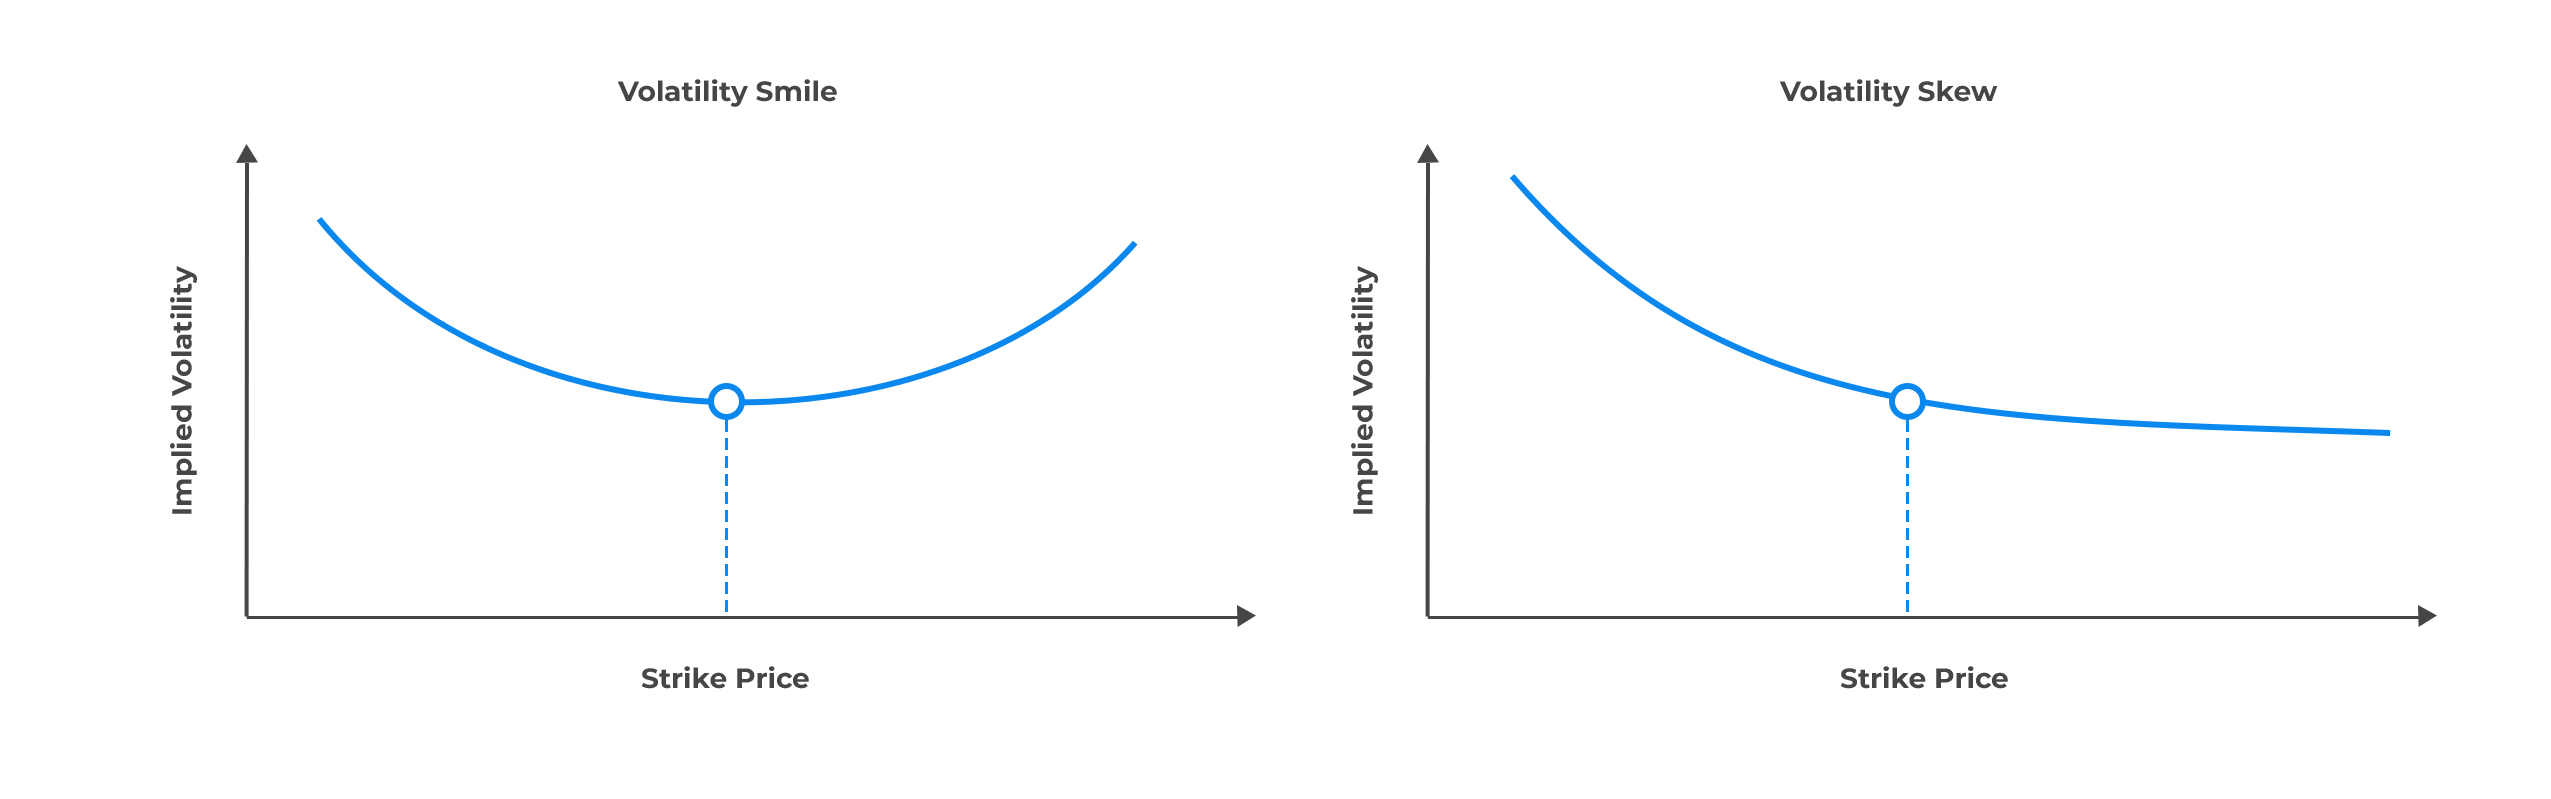
\includegraphics[width=0.9\textwidth]{images/smile_vs_smirk.png}
\end{center}


\subsubsection{Volatility Smile (Symmetric Shape)}

A volatility smile occurs when out-of-the-money (OTM) calls and puts have higher implied volatility than at-the-money (ATM) options.

Graphically, this produces a U-shaped curve, with the lowest implied volatility near the ATM strike and higher values on both tails.

\textbf{Key Intuition:} Each strike "sees" a different part of the future distribution
\begin{itemize}
\item ATM options $\approx$ sensitive to small, typical price moves.
\item Deep OTM puts $\approx$ sensitive to crashes / large downward moves.
\item Deep OTM calls $\approx$ sensitive to extreme upward rallies.
\end{itemize}

If the market believes that the tails of the distribution are heavier (fatter) than in the log-normal model, then:
\begin{itemize}
\item OTM options become more valuable than Black–Scholes predicts.
\item To match the higher market price, the inverted Black–Scholes formula must use a higher implied volatility for OTM strikes.
\end{itemize}

\textbf{Why does a SMILE (symmetric) appear?}

In some markets (e.g. FX, commodities) price movements are relatively symmetric:
\begin{itemize}
\item Large upward moves are possible,
\item Large downward moves are possible,
\item The return distribution has fat tails on both sides ("snowball" effect).
\end{itemize}

Therefore:
\begin{itemize}
\item OTM puts are expensive $\rightarrow$ high IV,
\item OTM calls are expensive $\rightarrow$ high IV,
\item ATM options are less extreme $\rightarrow$ lower IV.
\end{itemize}

Result: U-shaped curve $\rightarrow$ volatility smile.

\subsubsection{Volatility Skew / Smirk (Asymmetric Shape)}

In equity and index markets (e.g. S\&P 500, Eurostoxx), the typical shape is not symmetric, but downward sloping.

\textbf{Market reality:}
"The market goes up the stairs and down the elevator."

\begin{itemize}
\item Prices rise slowly but fall quickly.
\item Crashes (large drops) are more likely than extreme rallies.
\item The left tail (negative returns) is much heavier than the right tail.
\end{itemize}

\textbf{Investor behavior amplifies this:}
\begin{itemize}
\item Investors are willing to pay a lot for protection against losses $\rightarrow$ strong demand for OTM puts.
\item Effects such as leverage effect, jump risk, and panic selling further increase downside risk.
\end{itemize}

\textbf{Consequences on option prices:}
\begin{itemize}
\item OTM puts = very expensive $\rightarrow$ implied volatility extremely high
\item ATM options = moderate exposure $\rightarrow$ medium implied volatility
\item OTM calls = low demand $\rightarrow$ low implied volatility
\end{itemize}

Result: a downward-sloping curve as strike increases $\rightarrow$ volatility skew (or smirk).

\newpage
\section{October 21, 2025}

\subsection{Greeks and Sensitivity Analysis}

Let $V(t, s, T, r, \sigma)$ be the value of a portfolio (for example, $V = C_{BS}$ for a call option or $V = -P_{BS}$ for a put option).

The Greeks measure the sensitivity of this portfolio to changes in the model parameters.

\subsubsection{Definition}

\begin{center}
\begin{tabular}{|c|c|c|p{8cm}|}
\hline
\textbf{Greek} & \textbf{Symbol} & \textbf{Definition} & \textbf{Interpretation} \\
\hline
Delta & $\Delta$ & $\Delta = \frac{\partial V}{\partial S}$ & Sensitivity of the option value to changes in the underlying price. \\
\hline
Gamma & $\Gamma$ & $\Gamma = \frac{\partial^2 V}{\partial S^2}$ & Sensitivity of Delta to changes in the underlying (curvature). \\
\hline
Rho & $\rho$ & $\rho = \frac{\partial V}{\partial r}$ & Sensitivity of the option value to changes in the interest rate. \\
\hline
Theta & $\Theta$ & $\Theta = -\frac{\partial V}{\partial t}$ & Sensitivity of the option value to the passage of time (time decay). \\
\hline
Vega & $\nu$ & $\nu = \frac{\partial V}{\partial \sigma}$ & Sensitivity of the option value to changes in volatility. \\
\hline
\end{tabular}
\end{center}

A portfolio with a null Greek (e.g., $\Delta = 0$) is said to be \textbf{neutral} with respect to that Greek — i.e., insensitive to small changes in that parameter.

\subsubsection{Practical Interpretation of the Greeks}

The Greeks can be categorized based on their relationship to intrinsic and extrinsic value:

\begin{itemize}
\item \textbf{Intrinsic Value Components:} Delta and Gamma depend on the option's strike price relative to the underlying asset's price.
\item \textbf{Extrinsic Value Components:} Theta, Vega, and Rho are determined by time to expiration, volatility, and interest rates.
\end{itemize}

Vega is particularly important as an unknown variable, since implied volatility is forward-looking and cannot be predicted. \\
Regarding rho, Interest rates typically impact longer-dated options more significantly.

\paragraph{Delta}

Delta measures the amount an option's price should change based on a \$1 move up in the stock.

\begin{itemize}
\item \textbf{Call options} have a positive delta between 0 and 1
\item \textbf{Put options} have a negative delta between 0 and -1
\end{itemize}

Delta can also represent the number of relative shares you would own if you purchased an option at a specific delta. Buying a call option with a 0.30 delta is roughly equivalent to owning 30 shares of stock.

Additionally, Delta can act as an approximation of the probability an option will finish in-the-money. A 0.50 delta has roughly a 50\% chance of expiring in-the-money.

\begin{center}
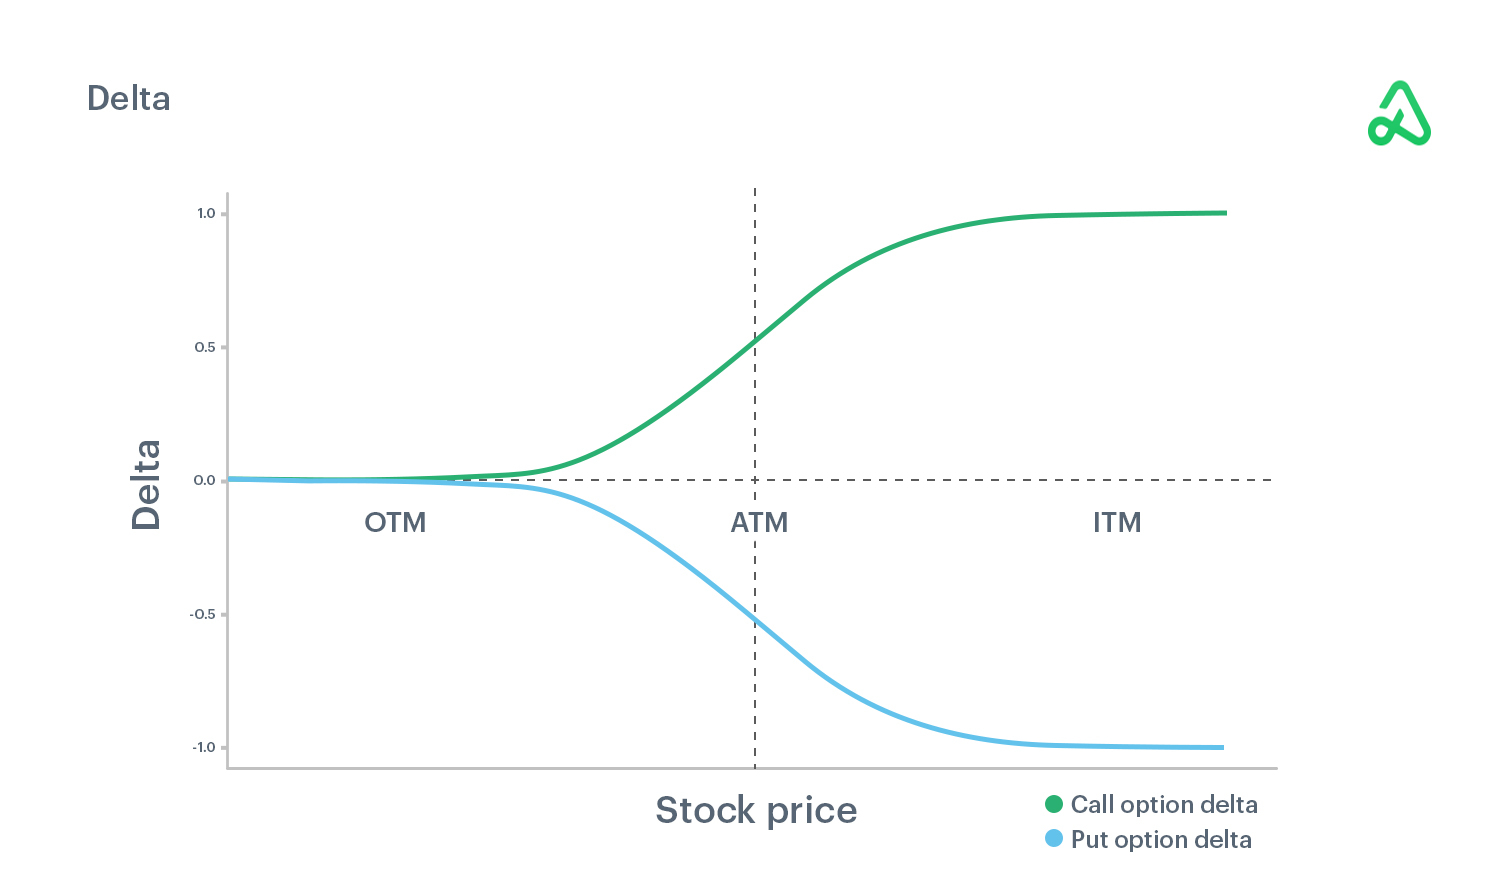
\includegraphics[width=0.7\textwidth]{images/delta.jpg}
\end{center}

\paragraph{Gamma}

Gamma is the rate of change in delta for every \$1 change in the underlying price. Gamma represents the acceleration at which an option's price increases or decreases. Think of gamma as the "next dollar move."

For example, if an option has a delta of 0.60 and a gamma of 0.10, the first dollar move in the underlying asset will see the price of the option change by \$0.60. The subsequent dollar move of the stock will see the price of the option change another \$0.60 plus an additional \$0.10 because of gamma.

Gamma is highest for contracts closer to at-the-money and declines as an option moves farther in-the-money or out-of-the-money.

\begin{center}
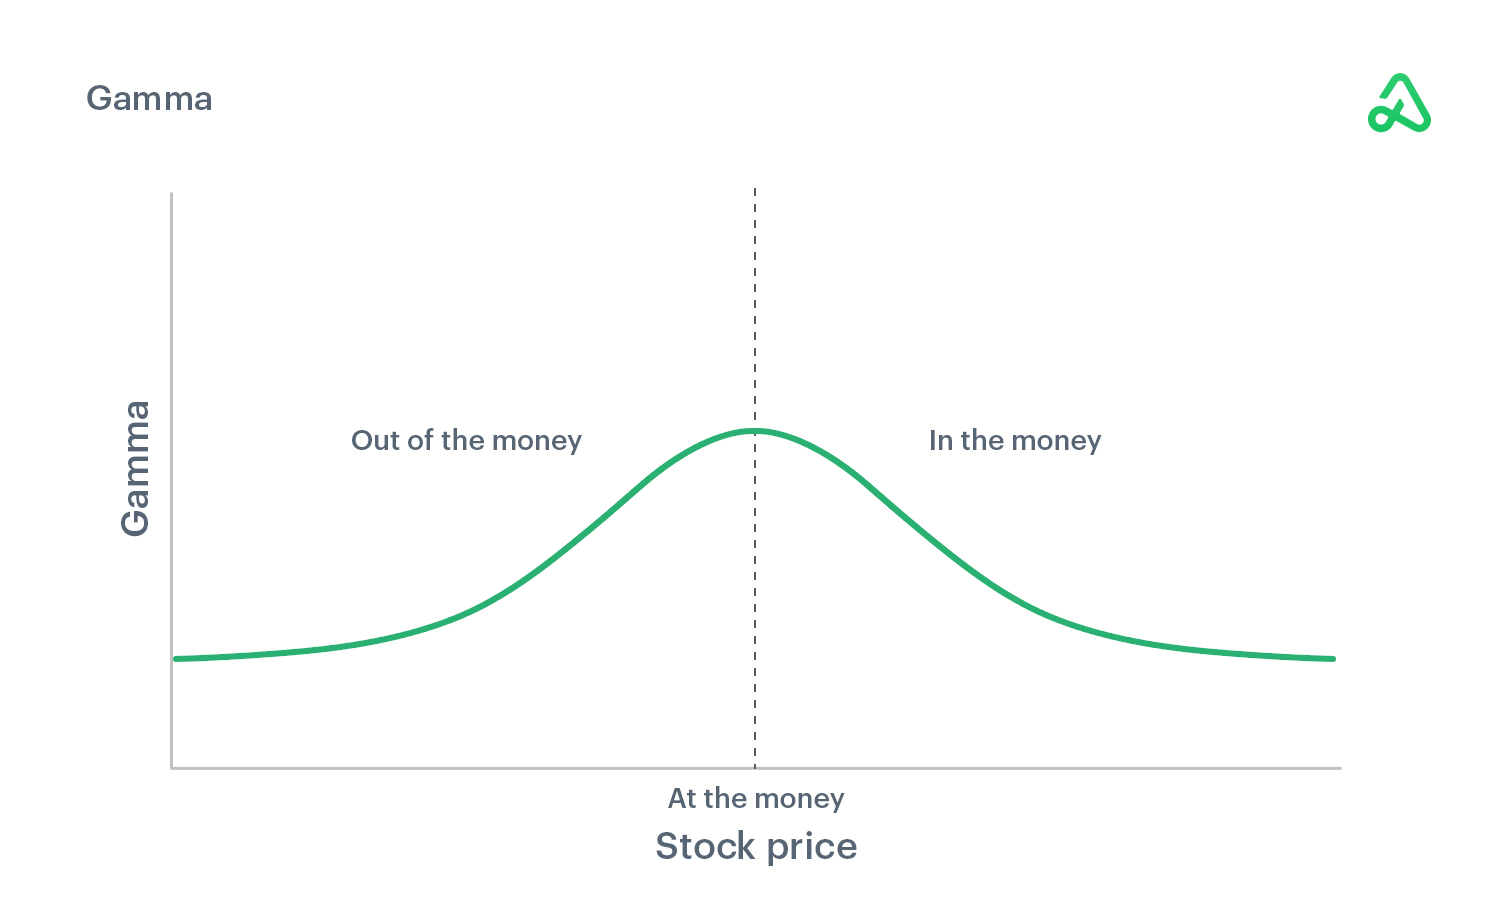
\includegraphics[width=0.7\textwidth]{images/gamma.jpg}
\end{center}

\paragraph{Theta}

Theta measures the effect time decay has on the value of an option. Options are a decaying asset and lose value every day, no matter what. Because of this, Theta is an advantage for the option seller and a disadvantage for the option buyer.

Theta is smaller on long-dated options but time decay accelerates as expiration approaches. The rate at which options contracts lose value increases exponentially.

Theta is the amount the price of the option will decrease each day and is always represented as a negative value. For example, a theta value of -0.04 means the option will lose \$0.04 each day.

\begin{center}
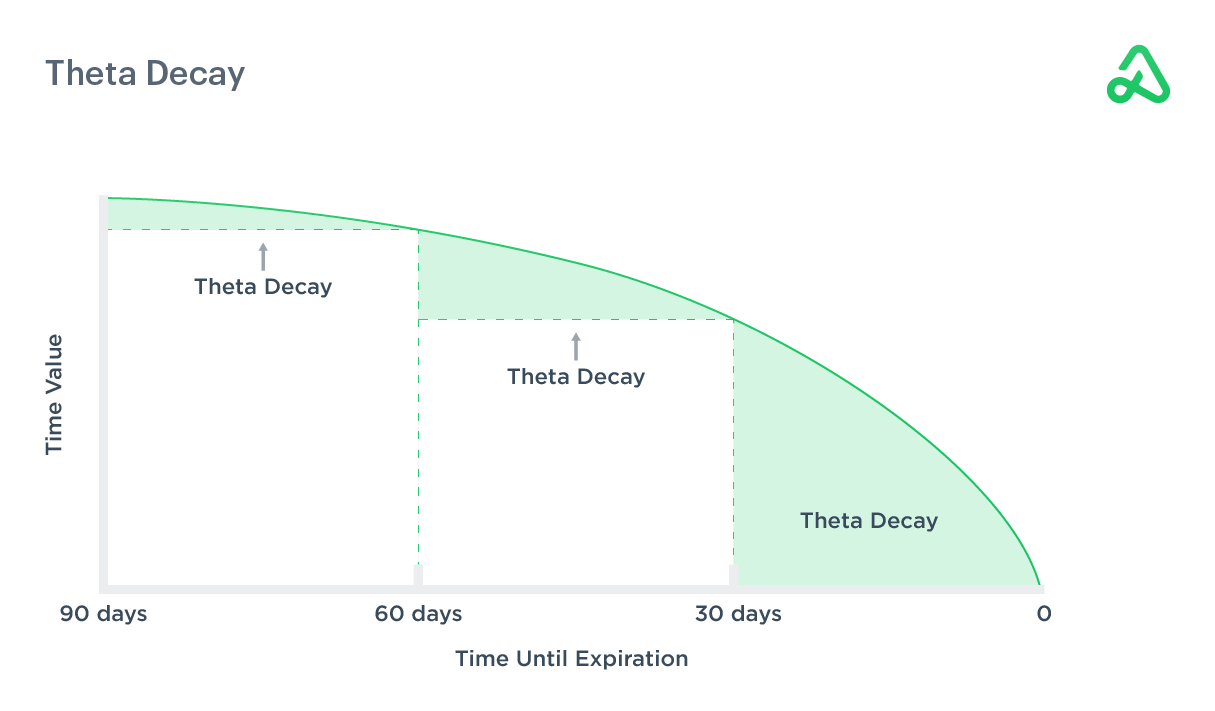
\includegraphics[width=0.7\textwidth]{images/theta.png}
\end{center}

\paragraph{Vega}

Vega measures the amount an option's value changes for a 1\% change in implied volatility in the underlying security. As volatility increases, an option's price goes up as market participants anticipate an above-average move may be coming. Vega declines as an option approaches expiration because there is less time for volatility to impact the option's value.

Unlike the other components of an option's price (spot price, strike price, and time to expiration), Vega is an unknown element because future volatility can't be predicted or forecasted. Therefore, Vega does not impact the intrinsic value because it is not based on the stock's changing price, only changes in volatility.

\begin{center}
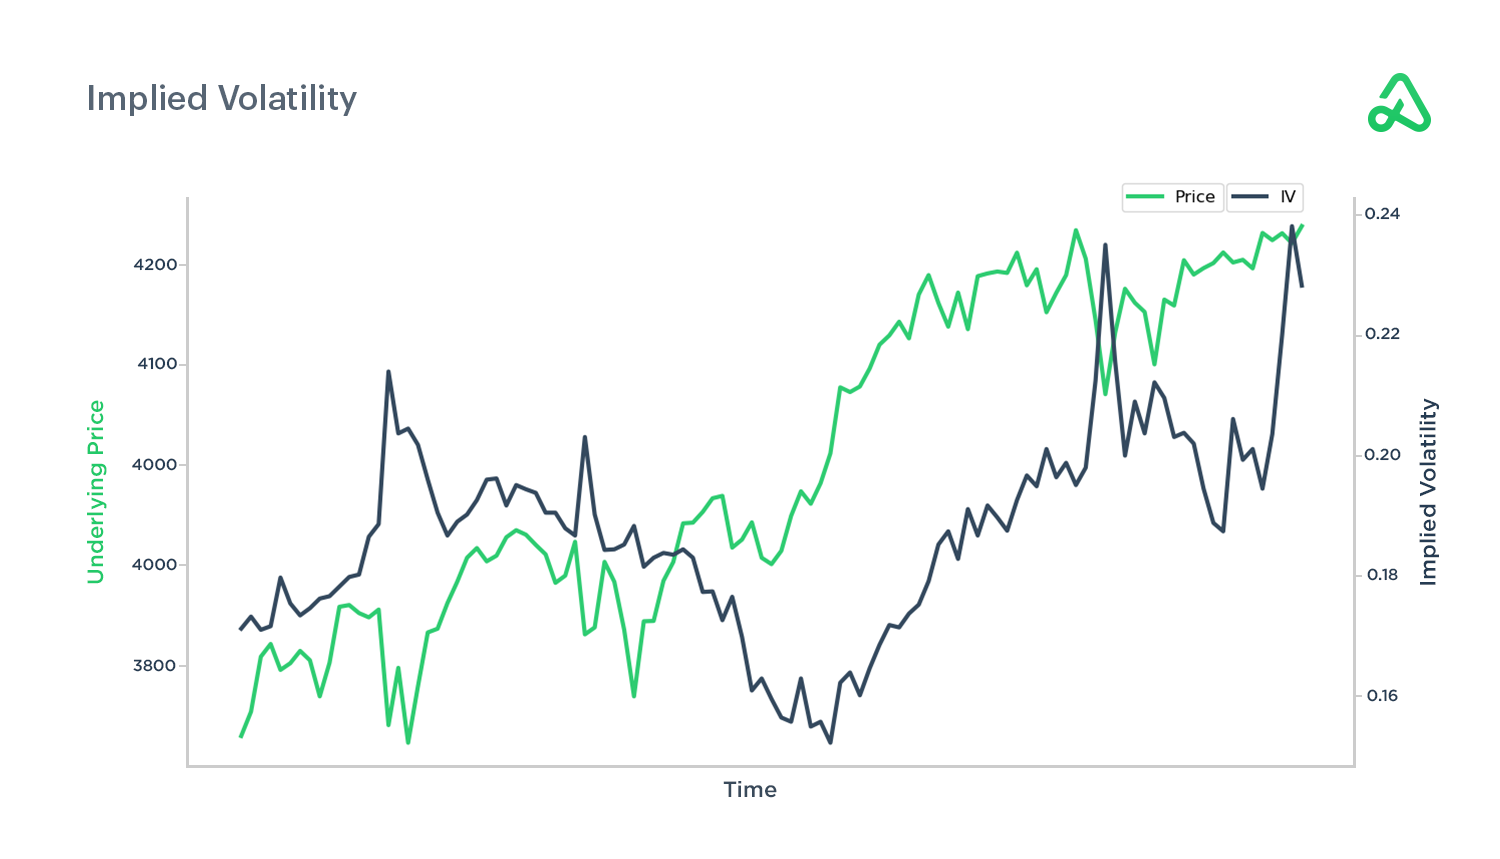
\includegraphics[width=0.7\textwidth]{images/vega.png}
\end{center}

\paragraph{Rho}

Rho measures an option's sensitivity to changes in interest rates. Rho represents the expected change of a contract's value for a 1\% change in interest rates. Rho is not as important for short-term options traders because changes in interest rates are usually relatively small, and only adjusted once per quarter, if at all.

\subsubsection{Greeks for the European Call Option}

For a European call option under the Black–Scholes model, we have:

\begin{center}
\fbox{\parbox{0.9\textwidth}{\centering
\vspace{0.5em}
\textbf{Black–Scholes Greeks for European Call:}
\begin{align*}
\Delta &= N(d_1), \\
\\
\Gamma &= \frac{\phi(d_1)}{s\sigma\sqrt{T-t}}, \\
\\
\rho &= K(T-t)e^{-r(T-t)}N(d_2), \\
\\
\Theta &= -\frac{s\sigma\phi(d_1)}{2\sqrt{T-t}} - rKe^{-r(T-t)}N(d_2), \\
\\
\nu &= s\phi(d_1)\sqrt{T-t}.
\end{align*}
}}
\end{center}

where:
\[
d_1 = \frac{\ln(s/K) + (r + \frac{1}{2}\sigma^2)(T-t)}{\sigma\sqrt{T-t}}, \quad d_2 = d_1 - \sigma\sqrt{T-t}.
\]

\subsubsection{Remarks}

\begin{itemize}
\item The price of $C_{BS}$ increases with $s, \sigma, r$, and decreases with $t$.
\item The portfolio used in the Black–Scholes derivation is Delta-neutral.
\end{itemize}

Indeed, the hedging portfolio is:
\[
V(t,s) = C_{BS}(t,s) - yS_t.
\]

Then:
\[
\frac{\partial V}{\partial S} = N(d_1) - y = 0 \quad \Longrightarrow \quad y = N(d_1) = \Delta.
\]

Hence, $y$ represents the number of shares required to make the portfolio Delta-neutral.

\subsection{Buy \& Hold Strategy (Replication)}

To replicate contingent claims, we combine basic traded assets:

\begin{center}
\begin{tabular}{|c|c|c|}
\hline
\textbf{Asset} & \textbf{Payoff at $T$} & \textbf{Value at time $t$} \\
\hline
Bond & $\Phi_B = 1$ & $\Pi_t(\Phi_B) = e^{-r(T-t)}$ \\
\hline
Stock & $\Phi_S = S_T$ & $\Pi_t(\Phi_S) = S_t$ \\
\hline
European Call & $\Phi_{C,K}(X) = [X - K]^+$ & $\Pi_t(\Phi_{C,K}) = c(t, S_t, K, T)$ \\
\hline
\end{tabular}
\end{center}

\subsubsection{Replication of a Contingent Claim}

Suppose we have a contingent claim $X = \Phi(S_T)$.

We aim to replicate it via a Buy \& Hold (B\&H) strategy.

Assume:
\[
\Phi(S_T) = \alpha\Phi_S + \beta\Phi_B + \sum_{i=1}^n \gamma_i \Phi_{C,K_i},
\]
where:
\begin{itemize}
\item $\alpha$ = number of shares of the stock,
\item $\beta$ = number of bonds,
\item $\gamma_i$ = number of call options with strike $K_i$.
\end{itemize}

By construction, the portfolio consisting of $\alpha, \beta, \{\gamma_i\}$ replicates $\Phi(S_T)$.

Hence, its value at time $t$ is:
\[
\Pi_t(\Phi) = \alpha S_t + \beta e^{-r(T-t)} + \sum_{i=1}^n \gamma_i \, c(t, S_t, T, K_i).
\]

\subsubsection{Example: Replication of a European Put}

An European Put with maturity $T$ and strike $K$ can be replicated using:
\[
\alpha = -1, \quad \beta = K, \quad \gamma = 1.
\]

Then, its value is:
\[
\Pi_t(\Phi_P) = -S_t + Ke^{-r(T-t)} + c(t, S_t, T, K).
\]

This is precisely the Put–Call Parity:
\[
C_{BS} - P_{BS} = S_t - Ke^{-r(T-t)}.
\]

\subsection{Completeness in the Black–Scholes Model}

\subsubsection{Definition}

A contingent claim $X$ maturing at time $T$ can be hedged or replicated if there exists a self-financing portfolio $h = (h_t^B, h_t^S)$ such that
\[
V_T^h = X \quad \text{a.s. under } \Prob.
\]
In this case, $h$ is called a \textbf{replicating portfolio} for $X$.

A market is said to be \textbf{complete} if every contingent claim can be replicated by some self-financing trading strategy.

\subsubsection{Setting}

Let $X = \Phi(S_T)$ be a contingent claim depending only on the terminal stock price.

The key idea is that, under the no-arbitrage (NA) condition,
\[
\Pi_t(X) = V_t^h,
\]
i.e. the price of $X$ at time $t$ equals the value of the replicating portfolio at time $t$.

\subsubsection{Theorem (Black–Scholes Completeness)}

Assume $F \in C^{1,2}([0,T] \times (0,\infty))$ is a smooth function solving the Black–Scholes PDE:
\[
\begin{cases}
F_t + rsF_s + \frac{1}{2}\sigma^2 s^2 F_{ss} - rF = 0, \\
F(T,s) = \Phi(s).
\end{cases}
\]

Then the contingent claim $X = \Phi(S_T)$ can be replicated by the self-financing portfolio
\[
h = (h^B, h^S),
\]
where
\[
h_t^B = \frac{F(t, S_t) - S_t F_s(t, S_t)}{B_t}, \quad h_t^S = F_s(t, S_t).
\]

\subsubsection{Proof}

We verify that the portfolio $h$ is both self-financing and replicating.

By definition:
\[
\begin{cases}
dV_t^h = h_t^B \, dB_t + h_t^S \, dS_t & \text{(Self-financing condition)} \\
V_T^h = F(T, S_T) & \text{(Replication condition)}
\end{cases}
\]

\paragraph{Step 1 – Dynamics of the Portfolio}

In the Black–Scholes model:
\[
dB_t = rB_t \, dt, \quad dS_t = \alpha S_t \, dt + \sigma S_t \, dW_t.
\]

Hence, the change in portfolio value is:
\[
dV_t^h = h_t^B \, dB_t + h_t^S \, dS_t = [rh_t^B B_t + \alpha h_t^S S_t] dt + \sigma h_t^S S_t \, dW_t.
\]

Substituting the expressions for $h_t^B$ and $h_t^S$:
\[
dV_t^h = [r(F - S_t F_s) + \alpha S_t F_s] dt + \sigma S_t F_s \, dW_t.
\]

\paragraph{Step 2 – Using the PDE Relation}

From the Black–Scholes PDE:
\[
rF - rsF_s = F_t + \frac{1}{2}\sigma^2 s^2 F_{ss}.
\]

Substituting into the previous expression gives:
\[
dV_t^h = [F_t + \frac{1}{2}\sigma^2 S_t^2 F_{ss} + \alpha S_t F_s] dt + \sigma S_t F_s \, dW_t.
\]

\paragraph{Step 3 – Itô's Formula}

By Itô's Lemma, applied to $F(t, S_t)$:
\[
dF(t, S_t) = [F_t + \alpha S_t F_s + \frac{1}{2}\sigma^2 S_t^2 F_{ss}] dt + \sigma S_t F_s \, dW_t.
\]

Comparing the two expressions, we have:
\[
dV_t^h = dF(t, S_t).
\]

Thus, by construction, $V_t^h = F(t, S_t)$ for all $t$, and in particular:
\[
V_T^h = F(T, S_T) = \Phi(S_T).
\]

Hence the portfolio is self-financing and replicates $X$.

\begin{center}
\fbox{\parbox{0.8\textwidth}{\centering
\vspace{0.5em}
\textbf{Key Result:}
\[
V_t^h = F(t, S_t) = \Pi_t(X)
\]
The replicating portfolio value equals the derivative price at all times.
\vspace{0.5em}
}}
\end{center}

\subsubsection{Remark}

The relative composition of the replicating portfolio (as fractions of total wealth) is given by:
\[
u_t^B = \frac{F - S_t F_s}{F}, \quad u_t^S = \frac{S_t F_s}{F}.
\]

These represent, respectively, the proportion of wealth invested in the bond and in the stock at time $t$.

\subsubsection{Intuition}

\begin{itemize}
\item The PDE solution $F(t,s)$ represents the time–price function of the derivative.
\item Its derivative $F_s = \Delta$ dictates how much stock to hold in the replicating strategy.
\item The remaining value $F - S_t F_s$ is invested in the risk-free bond.
\item The result $dV_t^h = dF(t, S_t)$ shows that following this strategy reproduces the exact same dynamics as the derivative value process.
\end{itemize}

Therefore, every contingent claim $\Phi(S_T)$ can be replicated via a self-financing portfolio — implying that the Black–Scholes market is complete.

\subsection{Multidimensional Stochastic Calculus}

Let $(\Omega, \mathcal{F}, \Prob)$ be a fixed, complete probability space.

\subsubsection{Definition – $d$-Dimensional Brownian Motion}

A stochastic process
\[
\underline{W} = \{\underline{W}_t\}_{t \geq 0}
\]
with values in $\R^d$ is called a $d$-dimensional Brownian motion (or Wiener process) if the following conditions hold:

\begin{enumerate}
\item $\underline{W}$ has continuous trajectories a.s.
\item $\underline{W}_0 = \underline{0}$.
\item The increments are independent:
\[
\underline{W}_t - \underline{W}_s \perp\!\!\!\perp \underline{W}_s, \quad \forall \, 0 \leq s < t.
\]
\item The increments are stationary Gaussian:
\[
\underline{W}_t - \underline{W}_s \sim \mathcal{N}(\underline{0}, (t-s)I_d),
\]
where $I_d$ is the $d \times d$ identity matrix.
\end{enumerate}

\subsubsection{Notation}

From now on, let
\[
\mathbb{F} = \mathbb{F}^{\underline{W}} = \{\mathcal{F}_t^{\underline{W}}\}_{t \geq 0}
\]
denote the natural filtration generated by $\underline{W}$, augmented to satisfy the usual conditions (right-continuity and completeness).

\subsubsection{Integrable Processes}

Let $\sigma = (\sigma_t^{ij})_{i=1,\ldots,n; \, j=1,\ldots,d}$ be an $\R^{n \times d}$-valued stochastic process, defined on $[a,b]$.

\begin{definition}[The Space $M^p(a,b)$]
We say that
\[
\sigma \in M^p(a,b), \quad p \geq 1,
\]
if
\[
\E\left[\int_a^b |\sigma_t^{(i,j)}|^p \, dt\right] < +\infty, \quad \text{for all } i = 1, \ldots, n, \; j = 1, \ldots, d.
\]
That is, each component of $\sigma$ is $p$-integrable in time and square-integrable in expectation.
\end{definition}

\subsubsection{Multidimensional Stochastic Integral}

If $\sigma \in M^2(a,b)$, we define the stochastic integral of $\sigma$ with respect to the $d$-dimensional Brownian motion $\underline{W}$ as the $\R^n$-valued random variable:
\[
\int_a^b \sigma_t \, d\underline{W}_t := \left(\sum_{j=1}^d \int_a^b \sigma_t^{ij} \, dW_t^j\right)_{i=1,\ldots,n}.
\]

Each component of this vector is thus the sum of $d$ standard stochastic integrals, one for each component $W^j$ of the Brownian motion.

\subsubsection{Intuition}

\begin{itemize}
\item When $d = 1$, this definition reduces to the classical Itô integral $\int \sigma_t \, dW_t$.
\item When $d > 1$, each $W^j$ acts as an independent "source of randomness", and the process $\sigma$ defines how these random shocks are linearly combined to produce an $n$-dimensional outcome.
\end{itemize}

Hence,
\[
\int_a^b \sigma_t \, d\underline{W}_t
\]
is an $\R^n$-valued random variable capturing the accumulated effect of $d$ correlated (or independent) Brownian drivers over $[a,b]$.

\subsubsection{Example}

If $n = 2$ and $d = 3$, then:
\[
\sigma_t = \begin{pmatrix}
\sigma_t^{11} & \sigma_t^{12} & \sigma_t^{13} \\
\sigma_t^{21} & \sigma_t^{22} & \sigma_t^{23}
\end{pmatrix},
\]
and
\[
\int_a^b \sigma_t \, d\underline{W}_t = \begin{pmatrix}
\int_a^b \sigma_t^{11} dW_t^1 + \int_a^b \sigma_t^{12} dW_t^2 + \int_a^b \sigma_t^{13} dW_t^3 \\
\int_a^b \sigma_t^{21} dW_t^1 + \int_a^b \sigma_t^{22} dW_t^2 + \int_a^b \sigma_t^{23} dW_t^3
\end{pmatrix}.
\]

Each component of the output process mixes multiple sources of randomness weighted by the coefficients $\sigma_t^{ij}$.

\newpage
\section{November 3, 2025}

\subsection{Progressively Measurable Processes and Stochastic Integration}

\subsubsection{The Space $M^p(a,b)$ — General Definition}

Let $M^p(a,b)$, with $0 \leq a \leq b$ and $p \geq 1$, denote the class of progressively measurable processes with respect to $\mathbb{F}$, taking values in $\R^{m \times d}$, denoted by
\[
\sigma_t = (\sigma_t^{ij}), \quad i = 1, \ldots, m, \quad j = 1, \ldots, d
\]
(i.e., $m$ rows and $d$ columns), such that for all $i, j$:
\[
\E\left[\int_a^b |\sigma_t^{ij}|^p \, dt\right] < +\infty.
\]

\textbf{Intuition.} The space $M^p(a,b)$ consists of matrix-valued processes where each component is adapted to the filtration and has finite $p$-th moments when integrated over time. This ensures that stochastic integrals are well-defined.

\subsubsection{Multidimensional Stochastic Integral — Extended Formulation}

In particular, if $\sigma \in M^2(a,b)$, we define the following stochastic integral as an $\R^m$-valued vector:

\begin{center}
\fbox{\parbox{0.9\textwidth}{\centering
\vspace{0.5em}
\[
\int_a^b \sigma_t \, d\underline{W}_t := \left(\sum_{j=1}^d \int_a^b \sigma_t^{1j} \, dW_t^j, \; \ldots, \; \sum_{j=1}^d \int_a^b \sigma_t^{mj} \, dW_t^j\right).
\]
\vspace{0.5em}
}}
\end{center}

\textbf{Financial interpretation.} In our notation, $m$ refers to the number of financial assets traded in the market. Each of these assets may be influenced by a number of "random sources of noise" (the $d$ Brownian motions). The relation between these two dimensions plays a central role for market completeness:
We'll see that if $m = d$, the market is complete (each asset responds to a distinct source of randomness).

\subsection{Properties of Multidimensional Stochastic Integrals}

\subsubsection{Basic Property}

\begin{remark}
$\displaystyle \int_a^b \sigma_t \, d\underline{W}_t$ is an $\R^m$-valued random variable.
\end{remark}

Each component of this vector represents the accumulated stochastic contribution from all $d$ sources of randomness, weighted by the corresponding row of the matrix $\sigma_t$.

\subsubsection{Orthogonality of Stochastic Integrals}

\begin{proposition}[Orthogonality]
If $X^1, X^2 \in M^2(0, T)$, then for all $0 \leq s \leq t \leq T$:
\[
\E\left[\left(\int_s^t X_u^1 \, dW_u^1\right)\left(\int_s^t X_u^2 \, dW_u^2\right) \,\Big|\, \mathcal{F}_s\right] = 0.
\]
\end{proposition}

\textbf{Proof.} This follows from the independence of $W^1$ and $W^2$ and the martingale property of stochastic integrals with respect to independent Brownian motions.

\begin{corollary}
Define
\[
I_t^j := \int_0^t X_u^j \, dW_u^j.
\]
Then
\[
\text{Cov}(I_t^1, I_t^2) = \E[I_t^1 I_t^2] = 0,
\]
and the family $\{I_t^1, I_t^2\}_{t \in [0,T]}$ is a martingale.
\end{corollary}

\textbf{Intuition.} Stochastic integrals driven by different, independent Brownian motions are uncorrelated.

\subsubsection{Itô Isometry in Multiple Dimensions}

\begin{theorem}[Itô Isometry — Matrix Form]
Let $\sigma \in M^2(0, T)$. Then, for all $0 \leq s \leq t \leq T$:
\[
\E\left[\left|\int_s^t \sigma_u \, d\underline{W}_u\right|^2\right] = \E\left[\int_s^t |\sigma_u|^2 \, du\right] = \E\left[\int_s^t \text{Tr}(\sigma_u \sigma_u^\top) \, du\right],
\]
where for any $A = (a_{ij}) \in \R^{m \times d}$:
\[
|A|^2 = \sum_{i=1}^m \sum_{j=1}^d a_{ij}^2 = \text{Tr}(AA^\top).
\]
\end{theorem}

\textbf{Explanation of the trace formula.} The matrix product $\sigma_u \sigma_u^\top$ is an $m \times m$ matrix. Its trace equals the sum of all squared entries of $\sigma_u$:
\[
\text{Tr}(\sigma_u \sigma_u^\top) = \sum_{i=1}^m (\sigma_u \sigma_u^\top)_{ii} = \sum_{i=1}^m \sum_{j=1}^d (\sigma_u^{ij})^2 = |\sigma_u|^2.
\]

This is the natural generalization of the one-dimensional Itô isometry to the matrix-valued case.

\subsubsection{Stochastic Differential}

The construction is exactly the same as in the one-dimensional case, but now in multiple dimensions.

Let $\underline{X} = \{\underline{X}_t\}_{t \in [0,T]}$ be an $\R^m$-valued process.

Assume that there exists an initial deterministic value $x_0 \in \R^m$.

We require a drift and a diffusion coefficient, both vector-valued:
\[
\underline{\mu} \in M^1(0,T), \quad \underline{\sigma} \in M^2(0,T),
\]
such that each component of the process can be written as
\[
X_t^i = x_0^i + \int_0^t \mu_s^i \, ds + \sum_{j=1}^d \int_0^t \sigma_s^{ij} \, dW_s^j.
\]

If this holds for every $t \in [0,T]$ and every $i = 1, \ldots, m$, then we say that $\underline{X}$ admits a stochastic differential, which is written as
\[
dX_t^i = \mu_t^i \, dt + \underline{\sigma}_t^{\,i} \, d\underline{W}_t,
\]
where $\underline{\sigma}^{\,i}$ denotes the $i$-th row of $\underline{\sigma}$.

Here, the summation over $j$ in the definition above is interpreted as an inner-product-type operation: each component of the row is integrated with respect to the corresponding Brownian motion.

Equivalently, in a more compact vector form,
\[
d\underline{X}_t = \underline{\mu}_t \, dt + \underline{\sigma}_t \, d\underline{W}_t.
\]
with initial value
\[
\underline{X}_0 = \underline{x_0}.
\]

\subsubsection{Multidimensional Itô's Formula}

Consider $f \in C^{1,2}([0,T] \times \R^m)$ and let $\underline{X}$ be a process with stochastic differential
\[
d\underline{X}_t = \underline{\mu}_t \, dt + \underline{\sigma}_t \, d\underline{W}_t,
\]
with initial condition
\[
\underline{X}_0 = \underline{x_0}.
\]

Define the real-valued process $Z_t := f(t, \underline{X}_t)$.

Then $Z_t$ admits the following stochastic differential:
\[
\begin{aligned}
dZ_t = df(t, \underline{X}_t) = \Bigg\{ & f_t(t, \underline{X}_t) + \sum_{i=1}^m \mu_t^i \, f_{x_i}(t, \underline{X}_t) \\
& + \frac{1}{2} \sum_{i=1}^m \sum_{j=1}^m f_{x_i x_j}(t, \underline{X}_t) \, \underline{\sigma}_t^{\,i} (\underline{\sigma}_t^{\,j})^\top \Bigg\} dt \\
& + \sum_{i=1}^m f_{x_i}(t, \underline{X}_t) \, \underline{\sigma}_t^{\,i} \, d\underline{W}_t,
\end{aligned}
\]
where $\underline{\sigma}_t^{\,i}$ is the $i$-th row of $\underline{\sigma}_t$.

\paragraph{Comments — how each term corresponds to the 1D formula}

We still have a $dt$-part and a $dW$-part.

The space derivative multiplied by the drift becomes
\[
\sum_{i=1}^m \mu_t^i f_{x_i}(t, \underline{X}_t).
\]

The Itô correction term remains "$\frac{1}{2}$ second derivative $\times$ diffusion coefficient", but now the second derivative is a matrix of mixed partials $\rightarrow$ this produces the double sum in $i, j$.

For the diffusion term (the $dW$-part), the spatial derivatives are summed across all components.

\paragraph{Equivalent compact matrix representation}

There is an alternative way to express the same formula:
\[
\begin{aligned}
dZ_t = \Bigg\{ & f_t(t, \underline{X}_t) + D_x f(t, \underline{X}_t) \, \underline{\mu}_t \\
& + \frac{1}{2} \text{Tr}\big[D_x^2 f(t, \underline{X}_t) \, \underline{\sigma}_t \, \underline{\sigma}_t^\top\big] \Bigg\} dt \\
& + D_x f(t, \underline{X}_t) \, \underline{\sigma}_t \, d\underline{W}_t,
\end{aligned}
\]
where $D_x f$ denotes the gradient with respect to $x$, and $D_x^2 f$ the Hessian matrix with respect to $x$.

\subsubsection{Deriving the Itô Product Formula (Stochastic "Leibniz Rule") via an Example}

Let
\[
\underline{\mu} = \begin{bmatrix} \mu^1 \\ \mu^2 \end{bmatrix} \in M^1(0,T), \quad \underline{\sigma} = \begin{bmatrix} \underline{\sigma}^{\,1} \\ \underline{\sigma}^{\,2} \end{bmatrix} \in M^2(0,T), \quad \underline{W} = \begin{bmatrix} W^1 \\ \vdots \\ W^d \end{bmatrix}.
\]

Each row $\underline{\sigma}^{\,i}$ has $d$-components.

Consider the two-dimensional system
\[
\begin{cases}
dX_t^1 = \mu_t^1 \, dt + \underline{\sigma}_t^{\,1} \, d\underline{W}_t, \\
dX_t^2 = \mu_t^2 \, dt + \underline{\sigma}_t^{\,2} \, d\underline{W}_t.
\end{cases}
\]

Apply Itô's formula to $f(t, x_1, x_2) = x_1 x_2$:
\[
f(t, X_t^1, X_t^2) = X_t^1 X_t^2 \quad \Rightarrow \quad \text{Itô} \quad d(X_t^1 X_t^2) = \left\{X_t^2 \mu_t^1 + X_t^1 \mu_t^2 + \frac{1}{2} \cdot 2 \cdot \underline{\sigma}_t^{\,1} (\underline{\sigma}_t^{\,2})^\top\right\} dt + \left\{X_t^2 \underline{\sigma}_t^{\,1} + X_t^1 \underline{\sigma}_t^{\,2}\right\} d\underline{W}_t.
\]

From this we observe:
\[
X_t^2 (\mu_t^1 \, dt + \underline{\sigma}_t^{\,1} \, d\underline{W}_t) = X_t^2 \, dX_t^1
\]
\[
X_t^1 (\mu_t^2 \, dt + \underline{\sigma}_t^{\,2} \, d\underline{W}_t) = X_t^1 \, dX_t^2
\]

The remaining term is the quadratic covariation between $X^1$ and $X^2$:
\[
\langle X^1, X^2 \rangle_t = \int_0^t \underline{\sigma}_u^{\,1} (\underline{\sigma}_u^{\,2})^\top \, du, \quad \Rightarrow \quad d\langle X^1, X^2 \rangle_t = \underline{\sigma}_t^{\,1} (\underline{\sigma}_t^{\,2})^\top \, dt.
\]

\paragraph{Comments.}

\begin{itemize}
\item There is no time derivative (here $f_t = 0$).
\item The gradient w.r.t. $x_1$ is $x_2$, and w.r.t. $x_2$ is $x_1$.
\item The pure second derivatives vanish; only the mixed derivative survives.
\end{itemize}

\paragraph{Final product formula.}

\begin{center}
\fbox{\parbox{0.7\textwidth}{\centering
\vspace{0.5em}
\[
d(X_t^1 X_t^2) = X_t^1 \, dX_t^2 + X_t^2 \, dX_t^1 + d\langle X^1, X^2 \rangle_t.
\]
\vspace{0.5em}
}}
\end{center}

\subsubsection{Itô Formula in Quadratic-Variation Form}

For $f \in C^{1,2}$ and $\underline{X}$ with a stochastic differential:

\begin{center}
\fbox{\parbox{0.9\textwidth}{\centering
\vspace{0.5em}
\[
df(t, \underline{X}_t) = f_t(t, \underline{X}_t) \, dt + \sum_{i=1}^m f_{x_i}(t, \underline{X}_t) \, dX_t^i + \frac{1}{2} \sum_{i=1}^m \sum_{j=1}^m f_{x_i x_j}(t, \underline{X}_t) \, d\langle X^i, X^j \rangle_t.
\]
\vspace{0.5em}
}}
\end{center}

\subsection{Multidimensional Black--Scholes Model}

Consider a perfect market where the following assets are traded:

\textbf{A risk-free asset $B_t$}, with dynamics
\[
dB_t = B_t r \, dt.
\]

\textbf{$n$ risky assets $\underline{S} = (S^1, \ldots, S^n)$}, with dynamics
\[
dS_t^i = S_t^i(\alpha^i \, dt + \underline{\sigma}_t^{\,i} \, d\underline{W}_t), \quad S_0^i = s^i \in \R,
\]
where $\underline{\sigma} = (\sigma^{ij}) \in \R^{n \times d}$ is the volatility matrix, and $\underline{\alpha} = (\alpha^i) \in \R^n$ is the vector of local mean rates of return.

\begin{remark}
$\sigma^{ij}$ represents the "impact" of source of randomness $j$ on asset $i$.
\end{remark}

\subsubsection{Assumptions}

\begin{enumerate}
\item $r$, $\underline{\alpha}$, and $\underline{\sigma}$ are known constants.
\item $n = d$.
\item $\underline{\sigma}$ is non-singular.
\end{enumerate}

\subsubsection{Interpretation}

$\underline{W}$ is a source of randomness, in particular: "one risk factor" per Brownian component.

Assuming $n = d$ is justified by the Meta-Theorem:

Let $M$ be the number of traded risky assets and $R$ the number of sources of randomness. Then:
\begin{itemize}
\item The model is arbitrage-free $\Longleftrightarrow M \leq R$
\item The model is complete $\Longleftrightarrow M \geq R$
\end{itemize}

Therefore:

\begin{center}
\fbox{\parbox{0.7\textwidth}{\centering
\vspace{0.5em}
The model is arbitrage-free and complete $\Longleftrightarrow M = R$
\vspace{0.5em}
}}
\end{center}

(thus we impose $n = d$ for this reason).

\subsubsection{Multidimensional B\&S — Exchange Option Setup}

Consider a simple contingent claim of the form
\[
X = \Phi(\underline{S}_T).
\]

\textbf{Example (exchange option).}
\[
\Phi(\underline{S}_T) = \Phi(S_T^1, S_T^2) = \max\{S_T^2 - S_T^1, \, 0\}.
\]

Our aim is to determine its arbitrage-free price $\Pi_t(X)$ using the law of one price.

Since at maturity we must recover the payoff, we impose:
\[
\Pi_T(X) = \Phi(\underline{S}_T).
\]

\paragraph{Assumptions}

\begin{itemize}
\item The derivative is traded
\item No-arbitrage holds
\item $\Pi_t(X) = F(t, \underline{S}_t)$ for some sufficiently smooth function $F$
\end{itemize}

\paragraph{Portfolio Weights}

Let $h$ denote a portfolio with the following relative weights:
\begin{itemize}
\item $u_t^B$: fraction invested in the bank account
\item $u_t^i$: fraction invested in $S_t^i$
\item $u_t^F$: fraction invested in the derivative itself
\end{itemize}

Since the portfolio is fully invested:
\[
1 = u_t^B + \sum_{i=1}^n u_t^i + u_t^F \quad \Longleftrightarrow \quad u_t^B = 1 - \left(\sum_{i=1}^n u_t^i + u_t^F\right).
\]

\paragraph{Applying Itô's Formula to the Derivative Price}

By Itô:
\[
\begin{aligned}
dF(t, \underline{S}_t) = \Bigg\{ & F_t + \sum_{i=1}^n F_{S_i} S_t^i \alpha^i + \frac{1}{2} \sum_{i,j=1}^n F_{S_i S_j} \, S_t^i S_t^j \, \underline{\sigma}^{\,i} (\underline{\sigma}^{\,j})^\top \Bigg\} dt + \sum_{i=1}^n F_{S_i} S_t^i \, \underline{\sigma}^{\,i} \, d\underline{W}_t.
\end{aligned}
\]

\paragraph{We Construct a Self-Financing Portfolio $h$}

Let $V_t^h$ be the portfolio value. Self-financing implies
\[
\frac{dV_t^h}{V_t^h} = u_t^B \frac{dB_t}{B_t} + \sum_{i=1}^n u_t^i \frac{dS_t^i}{S_t^i} + u_t^F \frac{dF(t, \underline{S}_t)}{F(t, \underline{S}_t)}.
\]

Using $dB_t = B_t r \, dt$ and
\[
\frac{dS_t^i}{S_t^i} = \alpha^i \, dt + \underline{\sigma}_t^{\,i} \, d\underline{W}_t,
\]
together with Itô on $F(t, \underline{S}_t)$ with derivatives w.r.t. $\underline{S}$,
\[
\begin{aligned}
dF(t, \underline{S}_t) = \Bigg\{ & F_t + \sum_{i=1}^n F_{S_i}(\,t, \underline{S}_t) \, S_t^i \alpha^i + \frac{1}{2} \sum_{i,j=1}^n F_{S_i S_j}(\,t, \underline{S}_t) \, S_t^i S_t^j \, \underline{\sigma}_t^{\,i} (\underline{\sigma}_t^{\,j})^\top \Bigg\} dt \\
& + \sum_{i=1}^n F_{S_i}(\,t, \underline{S}_t) \, S_t^i \, \underline{\sigma}_t^{\,i} \, d\underline{W}_t,
\end{aligned}
\]
we can define the derivative's instantaneous return and volatility vector by
\[
\alpha_t^F := \frac{1}{F(t, \underline{S}_t)} \left[F_t + \sum_{i=1}^n F_{S_i} \, S_t^i \alpha^i + \frac{1}{2} \sum_{i,j=1}^n F_{S_i S_j} \, S_t^i S_t^j \, \underline{\sigma}_t^{\,i} (\underline{\sigma}_t^{\,j})^\top\right],
\]
\[
\underline{\sigma}_t^{\,F} := \frac{1}{F(t, \underline{S}_t)} \sum_{i=1}^n F_{S_i}(\,t, \underline{S}_t) \, S_t^i \, \underline{\sigma}_t^{\,i}.
\]

Hence
\[
\frac{dV_t^h}{V_t^h} = \left\{r + \sum_{i=1}^n u_t^i \, (\alpha^i - r) + u_t^F (\alpha_t^F - r)\right\} dt + \left\{\sum_{i=1}^n u_t^i \, \underline{\sigma}_t^{\,i} + u_t^F \, \underline{\sigma}_t^{\,F}\right\} d\underline{W}_t.
\]

\paragraph{Local Risk-Free Condition and No-Arbitrage}

To make $h$ locally risk-free (zero diffusion),
\[
\sum_{i=1}^n u_t^i \, \underline{\sigma}_t^{\,i} + u_t^F \, \underline{\sigma}_t^{\,F} = \underline{0}. \tag{$\bullet$}
\]

By no-arbitrage we require the drift of a locally risk-free strategy to equal $r$:
\[
\sum_{i=1}^n u_t^i \, (\alpha^i - r) + u_t^F \, (\alpha_t^F - r) = 0. \tag{$\bullet\bullet$}
\]

Putting ($\bullet$) and ($\bullet\bullet$) together yields the linear system
\[
\begin{bmatrix}
\alpha^1 - r & \cdots & \alpha^n - r & \alpha_t^F - r \\
(\underline{\sigma}_t^{\,1})^\top & \cdots & (\underline{\sigma}_t^{\,n})^\top & (\underline{\sigma}_t^{\,F})^\top
\end{bmatrix}
\begin{bmatrix}
u_t^1 \\
\vdots \\
u_t^n \\
u_t^F
\end{bmatrix}
=
\begin{bmatrix}
0 \\
\underline{0}
\end{bmatrix}.
\]

For non-trivial solutions, the matrix must be singular; equivalently, the first row is a linear combination of the others:

There exists $\underline{\Lambda}_t \in \R^d$ (the market price of risk) such that
\[
\alpha^i - r = \underline{\sigma}_t^{\,i} \, \underline{\Lambda}_t, \quad i = 1, \ldots, n,
\]
\[
\alpha_t^F - r = \underline{\sigma}_t^{\,F} \, \underline{\Lambda}_t.
\]

When $n = d$ and $\underline{\sigma}_t$ is non-singular, this gives
\[
\underline{\Lambda}_t = (\underline{\sigma}_t)^{-1} (\underline{\alpha} - r\underline{1}),
\]
and the derivative satisfies the same pricing relation.

\newpage
\section{November 4, 2025}

\subsubsection{Market Price of Risk — Interpretation}

The vector $\underline{\Lambda}$ is called the market price of risk.

It represents how much excess expected return an investor is compensated per unit of exposure to each Brownian source of randomness.

More precisely:
\begin{itemize}
\item $\Lambda^j$ is the "value" of one unit of excess return per unit of variation in the $j$-th Brownian factor.
\item $\sigma^{ij}$ measures the sensitivity (loading) of asset $i$ to risk factor $j$.
\end{itemize}

In this sense, the quantity $\frac{\alpha^i - r}{\sigma^{ij}}$ resembles a Sharpe ratio (excess return per unit of risk).

\subsubsection{Returning to the Pricing Equation}

Using $\underline{\sigma}^{\,F}$ and $\underline{\Lambda}$, the relation
\[
\alpha^i - r = \underline{\sigma}_t^{\,i} \, \underline{\Lambda}_t
\]
becomes, for the derivative,
\[
\alpha_t^F - r = \underline{\sigma}_t^{\,F} \, \underline{\Lambda}_t = \frac{1}{F(t, \underline{S}_t)} \sum_{i=1}^n F_{S_i}(t, \underline{S}_t) S_t^i \, \underline{\sigma}_t^{\,i} \, (\underline{\sigma}_t)^{-1} (\underline{\alpha} - r\underline{1}).
\]

After suitable algebraic manipulation, we arrive at the following fundamental result.

\begin{theorem}
Under the previous assumptions: frictionless complete market, $n = d$, $\underline{\sigma}$ non-singular, no-arbitrage, and the derivative traded, the pricing function $F(t, \underline{s})$ solves the PDE:
\[
F_t(t, \underline{s}) + \sum_{i=1}^n r s^i F_{S_i}(t, \underline{s}) + \frac{1}{2} \sum_{i=1}^n \sum_{j=1}^n s^i s^j \, \underline{\sigma}^{\,i} (\underline{\sigma}^{\,j})^\top \, F_{s_i s_j}(t, \underline{s}) - r F(t, \underline{s}) = 0
\]
with terminal condition
\[
F(T, \underline{s}) = \Phi(\underline{s}).
\]
\end{theorem}

\subsubsection{Risk-Neutral Valuation}

By the Feynman--Kac representation,
\[
F(t, \underline{x}) = \mathbb{E}\left[e^{-r(T-t)} \Phi(\underline{X}_T^{\,t,\underline{x}})\right],
\]
where $\underline{X}_t^{\,t,\underline{x}} = \underline{x}$ and
\[
dX_t^i = r \, dt + \underline{\sigma}^{\,i} \, d\underline{W}_t.
\]

But note: $X^i$ defined above is not equal to $S^i$ under the physical measure $\mathbb{P}$.

\textbf{Idea:} We want to construct a measure $\mathbb{Q} \sim \mathbb{P}$ such that
\[
dS_t^i = S_t^i(r \, dt + \underline{\sigma}^{\,i} \, d\underline{W}_t^\mathbb{Q}),
\]
for some Brownian motion $\underline{W}^\mathbb{Q}$ under $\mathbb{Q}$.

\subsubsection{Girsanov Theorem (Statement in This Context)}

Let $\underline{W}$ be a $d$-dimensional Brownian motion on $(\Omega, \mathcal{F}, \mathbb{F}, \mathbb{P})$, and $T > 0$.

Let $\underline{\varphi} \in M^2(0, T)$.

Define:
\[
L_t = \exp\left\{\int_0^t \underline{\varphi}_s \, d\underline{W}_s - \frac{1}{2} \int_0^t \|\underline{\varphi}_s\|^2 \, ds\right\}.
\]

Assume $L_t$ is a positive martingale.

Define the new measure $\mathbb{Q}$ by:
\[
\frac{d\mathbb{Q}}{d\mathbb{P}} = L_T.
\]

\textbf{Interpretation:}
\begin{itemize}
\item $\frac{d\mathbb{Q}}{d\mathbb{P}}$ is the Radon--Nikodym derivative: it rescales probabilities from $\mathbb{P}$ to $\mathbb{Q}$.
\item We are "tilting" the probability measure.
\end{itemize}

Then:
\[
\underline{W}_t^\mathbb{Q} = \underline{W}_t - \int_0^t \underline{\varphi}_s \, ds
\]
is a $d$-dimensional Brownian motion under $\mathbb{Q}$, and $\mathbb{Q} \sim \mathbb{P}$ (equivalent measures).

\subsubsection{Choosing the Shift}

Choose
\[
\underline{\varphi} = -\underline{\Lambda} = -(\underline{\sigma})^{-1} (\underline{\alpha} - r\underline{1}).
\]

Then
\[
d\underline{W}_t^\mathbb{Q} = d\underline{W}_t + (\underline{\sigma})^{-1} (\underline{\alpha} - r\underline{1}) \, dt.
\]

Hence,
\[
\underline{\alpha} \, dt + \underline{\sigma} \, d\underline{W}_t = \underline{\alpha} \, dt + \underline{\sigma} \, d\underline{W}_t^\mathbb{Q} - \underline{\sigma}(\underline{\sigma})^{-1} (\underline{\alpha} - r\underline{1}) dt = r\underline{1} \, dt + \underline{\sigma} \, d\underline{W}_t^\mathbb{Q}.
\]

Thus, under $\mathbb{Q}$,
\[
dS_t^i = S_t^i(r \, dt + \underline{\sigma}^{\,i} \, d\underline{W}_t^\mathbb{Q}).
\]

This is the risk-neutral dynamics.

\begin{definition}[Risk-Neutral Measure]
A probability measure $\mathbb{Q}$ on $(\Omega, \mathcal{F})$ is called risk-neutral if:
\begin{enumerate}
\item $\mathbb{Q} \sim \mathbb{P}$ (it is equivalent to the physical measure),
\item Under $\mathbb{Q}$, each risky asset satisfies
\[
dS_t^i = S_t^i(r \, dt + \underline{\sigma}^{\,i} \, d\underline{W}_t^\mathbb{Q}).
\]
\end{enumerate}
\end{definition}

\begin{theorem}[Risk-Neutral Valuation (Black--Scholes)]
Under all the previous assumptions (frictionless complete market, $n = d$, $\underline{\sigma}$ non-singular, the derivative is traded, and no-arbitrage holds), the no-arbitrage price $\Pi_t(X)$ of a contingent claim
\[
X = \Phi(\underline{S}_T)
\]
is given by
\[
\Pi_t(X) = F(t, \underline{S}_t) = \E^\mathbb{Q}\left[e^{-r(T-t)} \, \Phi(\underline{S}_T) \,\Big|\, \mathcal{F}_t\right].
\]
\end{theorem}

\begin{proposition}[Dynamics under the Risk-Neutral Measure]
In the Black--Scholes model, the price process $\Pi_t$ of any traded asset satisfies:

\textbf{Risk-neutral valuation formula}
\[
\Pi_t = \E^\mathbb{Q}\left[e^{-r(T-t)} \Pi_T \mid \mathcal{F}_t\right].
\]

\textbf{$\mathbb{Q}$-dynamics}

For some suitable volatility vector $\underline{\sigma}^\Pi$,
\[
d\Pi_t = \Pi_t(r \, dt + \underline{\sigma}_t^\Pi \, d\underline{W}_t^\mathbb{Q}).
\]

\textbf{Martingale property of the discounted price}

Defining $Z_t := \Pi_t / B_t$, we have
\[
Z_t \text{ is a } \mathbb{Q}\text{-martingale}.
\]
\end{proposition}

\subsection{State Space Reduction (Exchange Option)}

\textbf{Idea.} Exploit the homogeneity of the payoff $\Phi$ to make an educated guess (ansatz) for the functional form of $F$.

Consider a market with a risk-free asset and two risky assets $S^1, S^2$ whose (risk-neutral) dynamics are
\[
\begin{cases}
\dfrac{dS_t^1}{S_t^1} = r \, dt + \underline{\sigma}^{\,1} \, d\underline{W}_t, \\[0.5em]
\dfrac{dS_t^2}{S_t^2} = r \, dt + \underline{\sigma}^{\,2} \, d\underline{W}_t,
\end{cases}
\quad \underline{\sigma}^{\,i} \in \R^{1 \times d}.
\]

Consider the contingent claim
\[
X = \Phi(S_T^1, S_T^2) = [S_T^1 - S_T^2]^+,
\]
i.e., the option to exchange asset 2 for asset 1.

Since $\Phi$ is homogeneous of degree 1, $\Phi(a\underline{s}) = a \Phi(\underline{s})$.

Setting $z := s^1 / s^2$ and using $a = 1/s^2$,
\[
\Phi(s^1, s^2) = s^2 \, \Phi(z, 1).
\]

\subsubsection{Ansatz}

We therefore expect the price $F$ to inherit the same structure:
\[
F(t, s^1, s^2) = s^2 \, G(t, z), \quad z := \frac{s^1}{s^2}.
\]

\subsubsection{PDE for $F$}

The pricing PDE for $F$ is
\[
\begin{cases}
F_t + r s^1 F_{s_1} + r s^2 F_{s_2} + \dfrac{1}{2} \left[s_1^2 \, \|\underline{\sigma}^{\,1}\|^2 F_{s_1 s_1} + 2 s^1 s^2 \, \underline{\sigma}^{\,1} (\underline{\sigma}^{\,2})^\top F_{s_1 s_2} + s_2^2 \, \|\underline{\sigma}^{\,2}\|^2 F_{s_2 s_2}\right] - r F = 0, \\[0.5em]
F(T, s^1, s^2) = \Phi(s^1, s^2).
\end{cases}
\]

\subsubsection{Express Derivatives of $F$ in Terms of $G$}

With $F(t, s^1, s^2) = s^2 G(t, z)$, $z = s^1/s^2$, one obtains
\[
\begin{aligned}
F_t &= s^2 G_t, \quad F_{s_1} = G_z, \quad F_{s_2} = G - z G_z, \\
F_{s_1 s_1} &= \frac{1}{s^2} \, G_{zz}, \quad F_{s_1 s_2} = -\frac{z}{s^2} \, G_{zz}, \quad F_{s_2 s_2} = \frac{z^2}{s^2} \, G_{zz}.
\end{aligned}
\]

Moreover, the terminal payoff becomes
\[
G(T, z) = [z - 1]^+,
\]
i.e., the payoff of a call option on $z$ with strike 1.

\subsubsection{PDE for $G$}

Substituting the derivatives into the PDE for $F$ yields the one-dimensional boundary-value problem
\[
\begin{cases}
G_t + \dfrac{1}{2} \, z^2 \, \Sigma^2 \, G_{zz} = 0, \\[0.5em]
G(T, z) = [z - 1]^+,
\end{cases}
\]
where
\[
\Sigma^2 := s_1^2 \, \|\underline{\sigma}^{\,1}\|^2 F_{s_1 s_1} + 2 s^1 s^2 \, \underline{\sigma}^{\,1} (\underline{\sigma}^{\,2})^\top F_{s_1 s_2} + s_2^2 \, \|\underline{\sigma}^{\,2}\|^2 F_{s_2 s_2}.
\]

\subsubsection{Solution}

The solution is the Black--Scholes call price (with underlying $z$, strike 1, volatility $\Sigma$):
\[
G(t, z) = z \, N(d_1) - N(d_2),
\]
\[
d_1 = \frac{\ln z + \frac{1}{2}\Sigma^2(T-t)}{\Sigma\sqrt{T-t}}, \quad d_2 = d_1 - \Sigma\sqrt{T-t},
\]
where $N(\cdot)$ is the standard normal cdf.

Therefore, the exchange option price (Margrabe) is
\[
F(t, s^1, s^2) = s^2 \, G(t, z) = s^1 \, N(d_1) - s^2 \, N(d_2).
\]

\newpage
\section{November 6, 2025}

\subsection{Market Incompleteness and Factor Models}

\subsubsection{Meta-Theorem}

If $M < R$ then the market is incomplete, where $M$ denotes the number of traded assets and $R$ the number of independent risk factors driving the dynamics.

\textbf{Core intuition:} Dynamic replication requires one traded source of risk for each independent source of uncertainty. If there are fewer traded assets than risk factors, at least one source of randomness cannot be hedged, therefore perfect replication is impossible $\Rightarrow$ market incompleteness.

\subsubsection{Example: Factor Models}

Non-traded objects may be modelled as stochastic processes that indirectly influence the prices of traded assets and derivatives (their dynamics enter the coefficients of the SDEs of the traded instruments).

A factor can be:
\begin{itemize}
\item an observed quantity
\item an unobserved quantity $\Rightarrow$ in this case one must estimate the latent factor via probabilistic filtering techniques
\end{itemize}

\paragraph{Example 1: Short Rate Model}

Assume that the short rate evolves as
\[
dr_t = \mu(t, r_t) \, dt + \sigma(t, r_t) \, dW_t,
\]
but $r$ is not traded. Hence $M = 0$, $R = 1$ $\Rightarrow$ incompleteness.

\paragraph{Example 2: Temperature Derivatives}

Assume $X_t$ is the temperature somewhere:
\[
dX_t = \mu(t, X_t) \, dt + \sigma(t, X_t) \, dW_t.
\]

$X$ is clearly not traded.

Suppose $Y := \Phi(X_t)$. We cannot apply Black--Scholes in this incomplete market.

Assume that we also have $Z := \Gamma(X_t)$ and that this contract is traded.

To avoid arbitrage the prices must be market-consistent, meaning
\[
\Pi_t(Y) = F(t, X_t), \quad \Pi_t(Z) = G(t, X_t).
\]

Here $F(t, X_t)$ and $G(t, X_t)$ are the Mark-to-Market prices of the derivative contracts whose terminal payoff depends on $X_T$.

\subsection{Black--Scholes Argument in Incomplete Markets}

In a market with $(B, F, G)$ $\Rightarrow$ a self-financing portfolio using $F, G$ "kills volatility", forcing the local rate of return to be $r$.

By Itô:
\[
dF(t, X_t) = dF = F\{\alpha_t^F \, dt + \sigma_t^F \, dW_t\}
\]
where
\[
\alpha_t^F = \frac{1}{F}\left\{F_t + \mu F_x + \frac{\sigma^2}{2} F_{xx}\right\}, \quad \sigma_t^F = \frac{1}{F} \sigma F_x.
\]

Similar expressions hold for $G$.

\subsubsection{Relative Self-Financing Portfolio}

$h_t = (u_t^F, u_t^G)$ such that $u_t^F + u_t^G = 1$, where the weights $u_t^F, u_t^G$ represent fractions of total wealth allocated to each asset.

\[
dV_t^h = V_t^h\left\{u_t^F \frac{dF}{F} + u_t^G \frac{dG}{G}\right\} = V_t^h\{u_t^F \alpha_t^F + u_t^G \alpha_t^G\} \, dt + V_t^h\{u_t^F \sigma_t^F + u_t^G \sigma_t^G\} \, dW_t.
\]

We now have the system
\[
\begin{cases}
u_t^F + u_t^G = 1 \\
u_t^F \sigma_t^F + u_t^G \sigma_t^G = 0 \quad \text{(riskless: kill volatility)}
\end{cases}
\quad \Rightarrow \quad
\begin{cases}
u_t^F = -\dfrac{\sigma_t^G}{\sigma_t^F - \sigma_t^G} \\[0.5em]
u_t^G = \dfrac{\sigma_t^F}{\sigma_t^F - \sigma_t^G}.
\end{cases}
\]

Thus
\[
dV_t^h = V_t^h \frac{\alpha_t^G \sigma_t^F - \alpha_t^F \sigma_t^G}{\sigma_t^F - \sigma_t^G} \, dt.
\]

By NA:
\[
\frac{\alpha_t^G \sigma_t^F - \alpha_t^F \sigma_t^G}{\sigma_t^F - \sigma_t^G} = r \quad \Longleftrightarrow \quad \frac{\alpha_t^F - r}{\sigma_t^F} = \frac{\alpha_t^G - r}{\sigma_t^G}.
\]

Essentially the Sharpe ratios of $F$ and $G$ must coincide.

\subsection{Market Price of Risk}

This ratio is constant regardless of the specific derivative. Define
\[
\lambda = \lambda(t, x) := \frac{\alpha^F(t, X_t) - r}{\sigma^F(t, X_t)}
\]
the market price of risk.

\textbf{Clarification:} The Sharpe ratio is an asset-level quantity, but in equilibrium they must all be equal to the same $\lambda$.

$\lambda$ is a characteristic of the market and is determined by supply and demand.

\subsubsection{Plugging $\alpha^F$ and $\sigma^F$ Inside}

\begin{proposition}
Under all previous assumptions (i.e. — the factor dynamics for $X_t$, the existence of traded $G$, the absence of arbitrage, and the existence of a market price of risk $\lambda$), the pricing function $F$ of $Y = \Phi(X_T)$ solves the PDE:
\[
\begin{cases}
F_t(t, x) + (\mu(t, x) - \lambda(t, x)\sigma(t, x))F_x(t, x) + \dfrac{\sigma^2(t, x)}{2} F_{xx}(t, x) - r F(t, x) = 0 \\[0.5em]
F(T, x) = \Phi(x)
\end{cases}
\]
\end{proposition}

A similar PDE holds for $G$.

\begin{remark}
All model coefficients are given, except for $\lambda$.
\end{remark}

\subsubsection{Feynman--Kac Representation}

By Feynman--Kac: for any given $\lambda$, define a measure $\mathbb{Q}$ such that
\[
dX_t = (\mu(t, x) - \lambda(t, x)\sigma(t, x)) \, dt + \sigma(t, x) \, dW_t^\mathbb{Q}.
\]

Then
\[
F(t, x) = \E_{t,x}^\mathbb{Q}\left[e^{-r(T-t)} \Phi(X_T)\right].
\]

$\mathbb{Q}$ is not unique — it depends on the choice of $\lambda$.

\subsubsection{Factor Modelling with $k > 1$ Factors $X^1, \ldots, X^k$}

We have $X^j$ following SDEs driven by $n$ independent Brownian motions, and we have a risk-free asset $B$.

Assume there exists a liquid market with:
\begin{itemize}
\item $n$ "benchmark" derivatives $Y^i = \Phi^i(\underline{X}_T)$ and we assume $\Pi_t(Y^i) = F^i(t, \underline{X}_t)$.
\item A derivative we aim to price consistently: $Y = \Phi(\underline{X}_T)$ with $\Pi_t(Y) = F(t, \underline{X}_t)$.
\end{itemize}

Repeat the multi-dimensional Black--Scholes argument.

We find a market price of risk vector $\underline{\lambda} \in \R^n$ $\Rightarrow$ PDE + risk-neutral valuation formula.

($\mathbb{Q}$ is not unique.)

\subsection{The Martingale Approach}

This is the general framework that replaces the PDE approach.

Instead of building "local riskless" portfolios, we change numéraire and work in the discounted economy.

\textbf{General case:} Let $S^0, S^1, \ldots, S^n$ be the price processes of $n+1$ traded assets.

\textbf{Assumption:} $S_t^0 > 0$ $\mathbb{P}$-a.s. for all $t \geq 0$.

We take $S^0$ as the numéraire.

We define relative prices (a.k.a. the Z-economy):
\[
Z_t^i = \frac{S_t^i}{S_t^0} \quad \Longleftrightarrow \quad \underline{Z}_t = \left(1, \, \frac{S_t^1}{S_t^0}, \ldots, \frac{S_t^n}{S_t^0}\right).
\]

\subsubsection{Meaning of "S-Economy" vs "Z-Economy"}

\begin{itemize}
\item \textbf{S-economy} = original prices expressed in nominal units
\item \textbf{Z-economy} = prices normalized by the numéraire $S^0$ (i.e. everything becomes discounted)
\end{itemize}

\textbf{Example:} If $S_t^0 = B_t = e^{rt}$ then
\[
\underline{Z}_t = \left(1, \, e^{-rt} S_t^1, \ldots, e^{-rt} S_t^n\right).
\]

\textbf{Assumption:} $\underline{S}$ has a stochastic differential.

\begin{definition}[Portfolio Strategy]
A portfolio strategy is an $(n+1)$-dimensional process $\underline{h}_t = (h_t^0, \ldots, h_t^n)$ which is $\mathbb{F}^S$-progressively measurable.
\end{definition}

\subsubsection{Comparison Table: S-Economy vs Z-Economy}

\begin{center}
\begin{tabular}{|l|c|c|}
\hline
\textbf{Concept} & \textbf{S-economy} & \textbf{Z-economy} \\
\hline
\hline
Value process & $\displaystyle V_t^{h,S} = \sum_{i=0}^n h_t^i S_t^i$ & $\displaystyle V_t^{h,Z} = \sum_{i=0}^n h_t^i Z_t^i = h_t^0 + \sum_{i=1}^n h_t^i Z_t^i$ \\[1.5em]
\hline
Self-financing & $\displaystyle dV_t^{h,S} = \sum_{i=0}^n h_t^i \, dS_t^i$ & $\displaystyle dV_t^{h,Z} = \sum_{i=1}^n h_t^i \, dZ_t^i$ \\[1.5em]
\hline
Arbitrage & $V_0^{h,S} = 0, \, V_t^{h,S} \geq 0, \, \mathbb{P}(V_t^{h,S} > 0) > 0$ & similar \\[0.5em]
\hline
Reachability of $X$ & $\exists h$ admissible s.t. $V_T^{h,S} = X$ $\mathbb{P}$-a.s. & similar \\[0.5em]
\hline
\end{tabular}
\end{center}

\vspace{1em}

\begin{remark}
$V_t^{h,S} / S_t^0 = V_t^{h,Z}$.
\end{remark}

\begin{definition}[Admissible Portfolio]
A portfolio $h$ is \textbf{admissible} if it is self-financing and $\exists \alpha > 0$ (possibly depending on $h$) such that
\[
V_t^{h,S} / S_t^0 = V_t^{h,Z} \geq -\alpha \quad \mathbb{P}\text{-a.s. for all } t \geq 0.
\]
\end{definition}

\newpage
\section{November 10, 2025}

\subsection{Model Calibration in Factor Models}

Let $X^1, \ldots, X^k$ be the underlying factors of the model, representing the main state variables of the economy or market (for example, interest rates, volatilities, or equity indices).

Each factor follows a stochastic differential equation (SDE) of the form:
\[
dX_t^i = \mu^i(t, \underline{X}_t) \, dt + \underline{\sigma}^i(t, \underline{X}_t) \, d\underline{W}_t,
\]
where $\underline{W}_t$ is an $n$-dimensional Brownian motion under the physical probability measure $\mathbb{P}$.

The drift and volatility terms may depend on a vector of model parameters:
\[
\mu^i = \mu^i(t, \underline{x}, \underline{\beta}), \quad \underline{\sigma}^i = \underline{\sigma}^i(t, \underline{x}, \underline{\beta}),
\]
where $\underline{\beta} \in \R^k$ denotes the vector of parameters that characterize the model (for example, volatility levels, mean reversion speeds, or correlations).

We consider $n$ benchmark derivatives whose price processes are given by:
\[
\Pi_t^i = F^i(t, \underline{X}_t, \underline{\beta}), \quad i = 1, \ldots, n.
\]

From these, we can infer the market price of risk vector:
\[
\underline{\lambda} = \underline{\lambda}(t, \underline{X}_t, \underline{\beta}).
\]

\subsection{Calibration Procedure for $\underline{\lambda}$}

At time $t = 0$, assume that the initial state of the factors is known:
\[
\underline{X}_0 = \underline{x}_0.
\]

Then the calibration proceeds as follows:

\subsubsection{Compute Theoretical Prices}

For each benchmark derivative, compute the model-implied price:
\[
\Pi_{0,\underline{\beta}}^i = F^i(0, \underline{x}_0, \underline{\beta}).
\]

\subsubsection{Collect Observed Market Prices}

Obtain the corresponding observed (market) prices:
\[
\Pi_{0,*}^i.
\]

\subsubsection{Estimate the Parameter Vector}

Choose $\hat{\underline{\beta}}$ such that the theoretical prices are as close as possible to the observed prices.

A common approach is Ordinary Least Squares (OLS):
\[
\hat{\underline{\beta}} = \arg\min_{\underline{\beta} \in \R^n} \left[\sum_i (\Pi_{0,\underline{\beta}}^i - \Pi_{0,*}^i)^2\right].
\]

Once the calibration is completed, the parameters are now "pinned down" to market data, yielding:
\[
\hat{\underline{\beta}} \quad \Rightarrow \quad \hat{\underline{\lambda}} = \underline{\lambda}(t, \underline{x}, \hat{\underline{\beta}}).
\]

Consequently, we define the corresponding risk-neutral measure as:
\[
\mathbb{Q} = \mathbb{Q}_{\hat{\underline{\lambda}}}.
\]

Under this calibrated measure $\mathbb{Q}$, we can compute the theoretical prices of any other derivative.

\begin{remark}
\textbf{Who determines the choice of $\mathbb{Q}(\underline{\lambda})$?}

The market itself determines it through observed prices.
\end{remark}

\subsection{Lemma (Invariance)}

\begin{lemma}[Invariance]
\begin{enumerate}
\item $\underline{h}$ is self-financing with respect to $\underline{S}$ if and only if it is self-financing with respect to $\underline{Z}$.

\item $X$ is $\underline{S}$-reachable if and only if $X / S_T^0$ is $\underline{Z}$-reachable.

\item Moreover, No-Arbitrage (NA) holds in the $\underline{S}$-economy if and only if it holds in the $\underline{Z}$-economy.
\end{enumerate}
\end{lemma}

\begin{proof}[Proof (of point 2)]
($\Rightarrow$) Direction:

Assume that
\[
S_t^0 = e^{rt} = B_t, \quad S_t^1 = S_t,
\]
with dynamics
\[
dS_t = S_t(\alpha \, dt + \sigma \, dW_t).
\]

Let $\underline{h} = (h_t^0, h_t^1)$ be an admissible strategy.

Then, under the $\underline{S}$-economy,
\[
dV_t^{S,\underline{h}} = h_t^0 \, dB_t + h_t^1 \, dS_t = (rB_t h_t^0 + \alpha S_t h_t^1) \, dt + h_t^1 S_t \sigma \, dW_t.
\]

Now, consider the corresponding discounted wealth process under $\underline{Z}$:
\[
dV_t^{Z,\underline{h}} = d\!\left(\frac{V_t^{S,\underline{h}}}{S_t^0}\right) = d(e^{-rt} V_t^{S,\underline{h}}).
\]

Applying Itô's lemma gives:
\[
\begin{aligned}
dV_t^{Z,\underline{h}} &= -r e^{-rt} V_t^{S,\underline{h}} \, dt + e^{-rt} \, dV_t^{S,\underline{h}} \\
&= -r e^{-rt} (h_t^0 B_t + h_t^1 S_t) \, dt + e^{-rt} (rB_t h_t^0 + \alpha S_t h_t^1) \, dt + e^{-rt} h_t^1 S_t \sigma \, dW_t.
\end{aligned}
\]

Simplifying the $dt$-terms:
\[
dV_t^{Z,\underline{h}} = e^{-rt} h_t^1 S_t (\alpha - r) \, dt + e^{-rt} h_t^1 S_t \sigma \, dW_t.
\]

Note that:
\[
d(e^{-rt} S_t) = e^{-rt} S_t ((\alpha - r) \, dt + \sigma \, dW_t),
\]
so we can rewrite the wealth dynamics compactly as:
\[
\fbox{$dV_t^{Z,\underline{h}} = h_t^1 \, d(e^{-rt} S_t) = h_t^1 \, dZ_t,$}
\]
which shows that $\underline{h}$ is self-financing with respect to $\underline{Z}$.

\vspace{1em}

($\Leftarrow$) Direction:

Assume now that $\underline{h} = (h_t^0, h_t^1)$ is self-financing with respect to
\[
\underline{Z} = (Z_t^0, Z_t^1) = (1, e^{-rt} S_t).
\]

Then:
\[
V_t^{Z,\underline{h}} = h_t^0 Z_t^0 + h_t^1 Z_t^1 = h_t^0 + h_t^1 e^{-rt} S_t,
\]
and, since $Z_t^0 \equiv 1$ is constant,
\[
dV_t^{Z,\underline{h}} = h_t^1 \, dZ_t^1 = h_t^1 \, d(e^{-rt} S_t).
\]

Define the non-discounted wealth process:
\[
V_t^{S,\underline{h}} := S_t^0 V_t^{Z,\underline{h}} = e^{rt} V_t^{Z,\underline{h}}.
\]

We keep the same risky position $h_t^{1,S} := h_t^1$,
and define the risk-free holding in the $\underline{S}$-economy as:
\[
h_t^{0,S} := \frac{V_t^{S,\underline{h}} - h_t^{1,S} S_t}{S_t^0} = \frac{e^{rt} V_t^{Z,\underline{h}} - h_t^1 S_t}{e^{rt}}.
\]

Using Itô's product rule (noting that $S_t^0 = e^{rt}$ is deterministic):
\[
\begin{aligned}
dV_t^{S,\underline{h}} &= d(S_t^0 V_t^{Z,\underline{h}}) = V_t^{Z,\underline{h}} \, dS_t^0 + S_t^0 \, dV_t^{Z,\underline{h}} \\
&= r S_t^0 V_t^{Z,\underline{h}} \, dt + S_t^0 h_t^1 \, d(e^{-rt} S_t) \\
&= r V_t^{S,\underline{h}} \, dt + e^{rt} h_t^1 (e^{-rt} dS_t - r e^{-rt} S_t \, dt) \\
&= r(V_t^{S,\underline{h}} - h_t^1 S_t) \, dt + h_t^1 \, dS_t.
\end{aligned}
\]

Since $V_t^{S,\underline{h}} - h_t^1 S_t = S_t^0 h_t^{0,S}$, we have:
\[
dV_t^{S,\underline{h}} = r S_t^0 h_t^{0,S} \, dt + h_t^1 \, dS_t = h_t^{0,S} \, dS_t^0 + h_t^{1,S} \, dS_t.
\]

Hence, $\underline{h}$ is self-financing with respect to $\underline{S}$.
\end{proof}

\subsubsection{Reachability Equivalence}

If $X$ is $\underline{S}$-reachable, then $X / S_T^0$ is $\underline{Z}$-reachable:
simply discount the payoff and use the same strategy in discounted terms (self-financing invariance ensures consistency).

Conversely, if $X / S_T^0$ is $\underline{Z}$-reachable, then multiplying by $S_T^0$ gives a corresponding reachable payoff $X$ in the $\underline{S}$-economy, using the same risky holdings and the risk-free position defined as above.

\subsubsection{No-Arbitrage Equivalence}

Changing numéraire through the positive process $S^0$ is a one-to-one transformation between the $\underline{S}$-economy and the $\underline{Z}$-economy.

Since this transformation preserves both admissibility and sign of gains, we have:
\begin{itemize}
\item Any arbitrage in the $\underline{S}$-economy induces one in the $\underline{Z}$-economy (by discounting);
\item Any arbitrage in the $\underline{Z}$-economy induces one in the $\underline{S}$-economy (by reversing the discounting).
\end{itemize}

Therefore, \fbox{NA in $\underline{S}$ $\iff$ NA in $\underline{Z}$}.

\subsection{Equivalent Martingale Measures}

\subsubsection{Definitions}

\begin{definition}[Equivalent (Local) Martingale Measure — EMM/ELMM, relative to $S^0$]
A probability measure $\mathbb{Q}$ on $(\Omega, \mathcal{F})$ is an \textbf{equivalent (local) martingale measure} relative to the numéraire $S^0$ if:
\begin{enumerate}
\item $\mathbb{Q} \sim \mathbb{P}$ (i.e., $\mathbb{Q}$ is equivalent to $\mathbb{P}$); and
\item for every traded asset $i$, the discounted price process
\[
Z_t^i := \frac{S_t^i}{S_t^0}
\]
is a $\mathbb{Q}$-martingale (respectively, $\mathbb{Q}$-local martingale).
\end{enumerate}
\end{definition}

\begin{definition}[Local Martingale]
A process $M$ is a \textbf{local martingale} if there exists a sequence of stopping times $(\tau_n)_{n \geq 1}$ such that:
\begin{enumerate}
\item $\tau_n \uparrow +\infty$ a.s.; and
\item for every $n$, the stopped process $M_{t \wedge \tau_n}$ is a martingale.
\end{enumerate}
\end{definition}

\subsubsection{Propositions}

\begin{proposition}
If there exists an EMM $\mathbb{Q}$ (relative to $S^0$), then No-Arbitrage (NA) holds.

\textit{Remark:} in many texts this is stated under standard integrability/closedness assumptions; the stronger "NFLVR" is equivalent to the existence of an ELMM.
\end{proposition}

\begin{proposition}[Discounted dynamics under $\mathbb{Q}$]
Let $S^0 = B$ (the money-market account), and $S^1 = S$ as before. Then the discounted asset
\[
Z_t := \frac{S_t}{S_t^0}
\]
satisfies, under $\mathbb{Q}$,
\[
dZ_t = \sigma Z_t \, dW_t^\mathbb{Q},
\]
where $W^\mathbb{Q}$ is a $\mathbb{Q}$-Brownian motion.

\textit{Sketch:} apply Itô to $Z_t = e^{-rt} S_t$; under an EMM the drift of $Z$ vanishes, so only the diffusion term remains.
\end{proposition}

\subsubsection{NA via Contradiction under an EMM}

Assume, by contradiction, that there exists an admissible strategy $\underline{h}$ which is an arbitrage in the discounted economy $\underline{Z}$; i.e.
\[
V_t^{Z,\underline{h}} \geq 0 \text{ a.s. for all } t, \quad \mathbb{P}(V_T^{Z,\underline{h}} > 0) > 0 \iff \mathbb{Q}(V_T^{Z,\underline{h}} > 0) > 0,
\]
since $\mathbb{Q} \sim \mathbb{P}$. We will derive the contradiction $V_0^{Z,\underline{h}} > 0$.

Because $\underline{h}$ is self-financing in discounted units,
\[
dV_t^{Z,\underline{h}} = h_t^1 \, dZ_t = h_t^1 \, \sigma Z_t \, dW_t^\mathbb{Q},
\]
hence
\[
V_t^{Z,\underline{h}} = V_0^{Z,\underline{h}} + \int_0^t h_s^1 \, \sigma Z_s \, dW_s^\mathbb{Q},
\]
so $V^{Z,\underline{h}}$ is a $\mathbb{Q}$-local martingale. Since the strategy is admissible, $V^{Z,\underline{h}}$ is bounded from below, and every local martingale bounded from below is a $\mathbb{Q}$-supermartingale. Therefore,
\[
\mathbb{E}^\mathbb{Q}[V_t^{Z,\underline{h}} \mid \mathcal{F}_s] \leq V_s^{Z,\underline{h}}, \quad \forall \, 0 \leq s \leq t.
\]

Taking $s = 0$ and $t = T$ gives
\[
V_0^{Z,\underline{h}} \geq \mathbb{E}^\mathbb{Q}[V_T^{Z,\underline{h}}].
\]

But by assumption $V_T^{Z,\underline{h}} \geq 0$ a.s. and $\mathbb{Q}(V_T^{Z,\underline{h}} > 0) > 0$, hence
\[
\mathbb{E}^\mathbb{Q}[V_T^{Z,\underline{h}}] > 0 \quad \Longrightarrow \quad V_0^{Z,\underline{h}} > 0,
\]
contradicting the zero-initial-cost property required for an arbitrage strategy.

Therefore, no such $\underline{h}$ can exist, and NA holds under $\mathbb{Q}$.

\subsection{Weakening NA: Need for NFLVR}

For the converse implication ("existence of an ELMM $\Rightarrow$ NA"), the NA condition is sufficient.

However, for the reverse direction ("NA $\Rightarrow$ existence of an ELMM"), the classical NA condition is too weak.

We must replace NA with the stronger condition known as \textbf{No Free Lunch with Vanishing Risk (NFLVR)}.

Intuitively, if NFLVR does not hold, then we can construct a sequence of payoffs that behaves "almost" like an arbitrage.

More precisely, consider a bounded payoff $X \in L^\infty$ such that
\[
X \geq 0 \quad \mathbb{P}\text{-a.s.}, \quad \mathbb{P}(X > 0) > 0.
\]

If NFLVR fails, then there exists a sequence of payoffs $(X_n)$ such that:
\begin{itemize}
\item $X_n$ can be negative with positive probability,
\item each $X_n$ represents the payoff of a self-financing strategy,
\item the sequence approximates $X$ uniformly:
\[
|X - X_n| < \frac{1}{n} \quad \mathbb{P}\text{-a.s.},
\]
hence
\[
X_n \geq -\frac{1}{n} \quad \mathbb{P}\text{-a.s.}
\]
\item that is, we can approach a genuine arbitrage payoff arbitrarily closely, but without requiring bounded risk.
\end{itemize}

This is precisely the type of asymptotic arbitrage excluded by NFLVR.

\subsection{Fundamental Theorems of Asset Pricing}

\begin{theorem}[1FTAP — Delbaen \& Schachermayer]
Assume that the price process $\underline{S}$ is locally bounded (e.g., continuous trajectories). Then:
\[
\text{NFLVR} \quad \iff \quad \exists \, \mathbb{Q} \text{ ELMM}.
\]
\end{theorem}

\begin{theorem}[2FTAP]
Assume NFLVR and fix a numéraire $S^0$. Then the market is complete if and only if the ELMM $\mathbb{Q}$ relative to $S^0$ is unique.
\end{theorem}

\begin{remark}
The ELMM $\mathbb{Q}$ depends on the choice of the numéraire $S^0$.

Changing the numéraire generally produces a different equivalent martingale measure.
\end{remark}

\subsection{Pricing Approaches}

At this point, there are two complementary approaches to derivative pricing under NFLVR and an ELMM.

The first approach extends the market by assuming the derivative is itself tradable.

The second relies on replication and the law of one price.

Both methods lead to the same risk-neutral pricing formula.

\subsection{Martingale Pricing}

\subsubsection{First Approach: Extended Market}

Suppose we enlarge the market so that the contingent claim $X$ is itself a traded asset with price process $\Pi_t(X)$.

If NFLVR holds in this extended market, then there exists an ELMM $\mathbb{Q}$ such that:
\[
\frac{\Pi_t(X)}{S_t^0} \text{ is a } \mathbb{Q}\text{-local martingale}.
\]

Assume further that it is a true martingale (which holds under standard integrability conditions). Then:
\[
\frac{\Pi_t(X)}{S_t^0} = \mathbb{E}^\mathbb{Q}\left[\frac{\Pi_T(X)}{S_T^0} \mid \mathcal{F}_t\right] = \mathbb{E}^\mathbb{Q}\left[\frac{X}{S_T^0} \mid \mathcal{F}_t\right].
\]

Thus the general pricing formula is:
\[
\fbox{$\Pi_t(X) = S_t^0 \, \mathbb{E}^\mathbb{Q}\left[\frac{X}{S_T^0} \mid \mathcal{F}_t\right]$}
\]

In particular, if $S_t^0 = e^{rt}$, then:
\[
\fbox{$\Pi_t(X) = e^{-r(T-t)} \, \mathbb{E}^\mathbb{Q}[X \mid \mathcal{F}_t]$}
\]
which is exactly the risk-neutral pricing formula.

\subsubsection{Second Approach: Replication}

Assume instead that there exists a self-financing strategy $\underline{h}$ that replicates the claim $X$.

By the Law of One Price, the value of the strategy must coincide with the derivative price:
\[
V_t^{S,\underline{h}} = \Pi_t(X) \quad \iff \quad V_t^{Z,\underline{h}} = \frac{\Pi_t(X)}{S_t^0}.
\]

Under integrability, the discounted wealth process $V_t^{Z,\underline{h}}$ is a $\mathbb{Q}$-martingale.

Hence:
\[
\frac{\Pi_t(X)}{S_t^0} = \mathbb{E}^\mathbb{Q}\left[\frac{\Pi_T(X)}{S_T^0} \mid \mathcal{F}_t\right] = \mathbb{E}^\mathbb{Q}\left[\frac{X}{S_T^0} \mid \mathcal{F}_t\right],
\]
which yields again:
\[
\fbox{$\Pi_t(X) = S_t^0 \, \mathbb{E}^\mathbb{Q}\left[\frac{X}{S_T^0} \mid \mathcal{F}_t\right]$}.
\]

Thus both approaches agree.

\newpage
\section{November 11, 2025}

\subsection{Setting and Black--Scholes Dynamics}

Let $(\Omega, \mathcal{F}, \mathbb{P})$ be a complete probability space, carrying a Brownian motion $W$.

We assume the filtration is the augmented Brownian filtration:
\[
\mathbb{F} = \mathbb{F}^W.
\]

Fix a time horizon $T > 0$, and set $\mathcal{F} = \mathcal{F}_T$.

Consider the Black--Scholes model:
\[
\begin{cases}
dS_t = S_t(\alpha \, dt + \sigma \, dW_t), \\
dB_t = r B_t \, dt,
\end{cases}
\]
where $\sigma \neq 0$.

Thus the market has one risky asset $S = S^1$ and one riskless asset $B = S^0$, so $n = 1$.

The coefficients $\alpha, \sigma, r$ may also be time-dependent; nothing essential changes.

The only requirement is $\sigma_t \neq 0$, ensuring the asset is genuinely risky.

\subsection{Searching for an EMM: Girsanov's Theorem}

We seek an equivalent martingale measure $\mathbb{Q}$.

By Girsanov's theorem, to construct such a measure we look for a Girsanov kernel $h = (h_t)_t$ and consider the stochastic exponential
\[
\begin{cases}
dL_t = L_t \, h_t \, dW_t, \\
L_0 = 1.
\end{cases}
\]

If $L$ is a strictly positive martingale, we may define:
\[
\frac{d\mathbb{Q}}{d\mathbb{P}} = L_T.
\]

Under the measure $\mathbb{Q}$, the process
\[
W_t^\mathbb{Q} := W_t - \int_0^t h_s \, ds
\]
is a $\mathbb{Q}$-Brownian motion (by Girsanov).

\subsubsection{Transforming the SDE}

Using $dW_t = dW_t^\mathbb{Q} + h_t \, dt$, we obtain:
\[
dS_t = S_t(\alpha \, dt + \sigma \, dW_t^\mathbb{Q} + \sigma h_t \, dt) = S_t((\alpha + \sigma h_t) \, dt + \sigma \, dW_t^\mathbb{Q}).
\]

Thus $\mathbb{Q} \sim \mathbb{P}$, but we still must ensure that the discounted price is a $\mathbb{Q}$-martingale in order for $\mathbb{Q}$ to be an EMM.

\subsubsection{Martingale Condition for the Discounted Price}

The discounted asset is
\[
Z_t := \frac{S_t}{B_t} = e^{-rt} S_t.
\]

Compute its dynamics:
\[
dZ_t = e^{-rt} S_t (-r + \alpha + \sigma h_t) \, dt + e^{-rt} S_t \sigma \, dW_t^\mathbb{Q}.
\]

For $Z$ to be a $\mathbb{Q}$-martingale, the drift must be zero:
\[
-r + \alpha + \sigma h_t = 0 \quad \Longrightarrow \quad h_t = -\frac{\alpha - r}{\sigma} = -\lambda,
\]
the (negative) market price of risk.

In this model it is constant, so the Girsanov assumptions are automatically satisfied.

Thus we can define $\mathbb{Q}$ via the stochastic exponential with kernel $h_t = -\lambda$.

This $\mathbb{Q}$ is an EMM, and therefore:

\begin{theorem}
The Black--Scholes model is arbitrage-free.
\end{theorem}

\begin{remark}[General Coefficients]
The same result holds for time-dependent coefficients $\alpha_t, \sigma_t, r_t$, under standard conditions.

One obtains:
\[
h_t = -\frac{\alpha_t - r_t}{\sigma_t}.
\]

If $\sigma_t = 0$, then necessarily $\alpha_t = r_t$ (otherwise NA is violated).

In financial terms, the "risky" asset becomes riskless.

Therefore we require $\sigma_t \neq 0$ a.s. for all $t \geq 0$.
\end{remark}

\subsection{From Girsanov Kernel Back to the Measure}

Girsanov tells us: if we define the Radon--Nikodym derivative using a kernel $h$, we obtain an equivalent measure $\mathbb{Q}$ under which a shifted Brownian motion exists.

We now want the reverse direction:

\textit{Given an equivalent probability measure $\mathbb{Q}$, is it necessarily generated by a Girsanov kernel?}

\subsection{The Converse to Girsanov's Theorem}

\begin{theorem}[Converse to Girsanov]
Let $W$ be a Brownian motion on $(\Omega, \mathcal{F}, \mathbb{P})$, with $\mathbb{F} = \mathbb{F}^W$.

If $\mathbb{Q} \sim \mathbb{P}$, then there exists a unique kernel
\[
h \in M_{\text{loc}}^2(0, T)
\]
such that the density process
\[
Z_t := \frac{d\mathbb{Q}}{d\mathbb{P}}\Big|_{\mathcal{F}_t}
\]
satisfies:
\[
Z_t = \exp\left\{\int_0^t h_s \, dW_s - \frac{1}{2} \int_0^t h_s^2 \, ds\right\}.
\]
\end{theorem}

\begin{remark}
If the only source of randomness available to the market is a single Brownian motion $W$, then every equivalent change of measure is a Girsanov transformation.

In particular, if we want NA (i.e., the existence of an EMM), the Girsanov kernel is completely determined by the market coefficients.

Thus, in the Black--Scholes model, the Girsanov kernel is unique, the EMM is unique, and:
\end{remark}

\subsection{2FTAP for Black--Scholes}

\begin{theorem}
The Black--Scholes model is complete.

(Unique EMM $\iff$ every contingent claim is replicable.)
\end{theorem}

\subsection{Pricing a Contingent Claim}

Let $X$ be a contingent claim with maturity $T > 0$ and price process $\Pi_t(X)$.

The general risk-neutral pricing formula is:
\[
\Pi_t(X) = \mathbb{E}^\mathbb{Q}[e^{-r(T-t)} X \mid \mathcal{F}_t].
\]

It is more convenient to work in the discounted (Z-)economy:
\[
Z_t^0 = 1, \quad Z_t^1 = \frac{S_t}{B_t}, \quad \Pi_t^Z = \frac{\Pi_t}{B_t}.
\]

Our aim is to find a replicating portfolio $h = (h_t^0, h_t^1)$ such that:
\[
\begin{cases}
V_T^{Z,h} = \frac{X}{B_T} = e^{-rT} X, \\
dV_t^{Z,h} = h_t^1 \, dZ_t^1 \quad \text{(self-financing)}.
\end{cases}
\]

By the law of one price, we expect that the discounted value process satisfies:
\[
V_t^{Z,h} = \Pi_t^Z.
\]

\subsubsection{When is $\Pi^Z$ a $\mathbb{Q}$-martingale?}

If
\[
\frac{X}{B_T} \in L^1,
\]
then $\Pi_t^Z = \mathbb{E}^\mathbb{Q}\left[\frac{X}{B_T} \mid \mathcal{F}_t\right]$ is a \emph{true} $\mathbb{Q}$-martingale.

The justification is standard:
\begin{itemize}
\item The discounted payoff $X / B_T$ is integrable;
\item The process $\Pi_t^Z$ is the conditional expectation of an integrable random variable;
\item By the tower property,
\[
\mathbb{E}^\mathbb{Q}[\Pi_t^Z] = \mathbb{E}^\mathbb{Q}[X / B_T] < \infty;
\]
\item By Itô's formula applied to $\Pi_t^Z = e^{-rt} \Pi_t$, combined with the fact that the discounted asset $Z_t^1$ has zero drift under $\mathbb{Q}$, one obtains:
\[
d\Pi_t^Z = \text{(local martingale part)},
\]
and integrability ensures that it is a true martingale.
\end{itemize}

Thus:
\[
\fbox{$\Pi_t^Z$ is a $\mathbb{Q}$-martingale}.
\]

Under $\mathbb{Q}$:
\[
dZ_t^1 = d\!\left(\frac{S_t}{B_t}\right) = \sigma Z_t^1 \, dW_t^\mathbb{Q}.
\]

\subsection{The Martingale Representation Theorem (MRT)}

We now use the last major tool of stochastic calculus.

\begin{theorem}[Martingale Representation Theorem]
Let $M$ be a $(\mathbb{Q}, \mathbb{F})$-local martingale, where $\mathbb{F} = \mathbb{F}^W$.

Then there exist a unique constant $c \in \mathbb{R}$ and a unique process
\[
\psi \in M_{\text{loc}}^2(0, T)
\]
such that:
\[
M_t = c + \int_0^t \psi_s \, dW_s^\mathbb{Q}, \quad 0 \leq t \leq T.
\]
\end{theorem}

Apply this to the martingale $\Pi_t^Z$.

There exists a unique process $\psi_t$ such that:
\[
d\Pi_t^Z = \psi_t \, dW_t^\mathbb{Q}.
\]

But:
\[
d\Pi_t^Z = h_t^1 \, dZ_t^1 = h_t^1 \, \sigma Z_t^1 \, dW_t^\mathbb{Q}.
\]

Comparing the diffusion coefficients:
\[
\fbox{$h_t^1 = \frac{\psi_t}{\sigma Z_t^1}$}.
\]

This is the number of units invested in the risky asset $S$.

The cash holding follows from:
\[
V_t^Z = h_t^0 Z_t^0 + h_t^1 Z_t^1 = h_t^0 + h_t^1 Z_t^1,
\]
so:
\[
\fbox{$h_t^0 = V_t^Z - h_t^1 Z_t^1$}.
\]

\subsubsection{Verification of Replication}

We must still show that the strategy replicates the payoff.

At maturity:
\[
V_T^Z = \Pi_T^Z = \mathbb{E}^\mathbb{Q}\left[\frac{\Pi_T}{B_T} \mid \mathcal{F}_T\right] = \frac{X}{B_T},
\]
by the law of one price.

Thus the replication condition holds.

The only limitation is that the expression for $h_t^1$ is somewhat "abstract": it depends on $\psi_t$, whose explicit form may be unknown except for existence and uniqueness.

\subsection{Markovian Claims and Black--Scholes PDE}

If $X = \Phi(S_T)$ for some payoff function $\Phi$, then:
\[
\Pi_t(X) = \mathbb{E}^\mathbb{Q}[e^{-r(T-t)} \Phi(S_T) \mid \mathcal{F}_t] = \mathbb{E}^\mathbb{Q}[e^{-r(T-t)} \Phi(S_T) \mid S_t] = F(t, S_t),
\]
where $F(t, x)$ is a deterministic function (Markovianity).

Assuming $F \in C^{1,2}$, we can apply Itô's formula to
\[
\Pi_t^Z = e^{-rt} F(t, S_t).
\]

Compute:
\[
d\Pi_t^Z = \sigma \, e^{-rt} S_t \, F_s(t, S_t) \, dW_t^\mathbb{Q}.
\]

Hence:
\[
\psi_t = \sigma \, e^{-rt} S_t \, F_s(t, S_t).
\]

From the identification $h_t^1 = \psi_t / (\sigma Z_t^1)$ we obtain:
\[
h_t^1 = \frac{\sigma e^{-rt} S_t F_s(t, S_t)}{\sigma e^{-rt} S_t} = F_s(t, S_t).
\]

Thus:
\[
\fbox{$h_t^1 = F_s(t, S_t)$},
\]
the Delta of the option — exactly as expected.

Finally:
\[
h_t^0 = \frac{F(t, S_t)}{B_t} - F_s(t, S_t) \frac{S_t}{B_t} = \frac{F(t, S_t) - S_t F_s(t, S_t)}{B_t}.
\]

\subsection{Multidimensional Black--Scholes Model}

Consider a market with $n$ risky assets and one riskless asset.

The dynamics are:
\[
\begin{cases}
dS_t^i = S_t^i(\alpha^i \, dt + \underline{\sigma}^{\,i} \, d\underline{W}_t), \quad i = 1, \ldots, n, \\
dB_t = r B_t \, dt,
\end{cases}
\]
where:
\begin{itemize}
\item $\underline{W}$ is a $d$-dimensional Brownian motion,
\item $\underline{\alpha} = (\alpha^1, \ldots, \alpha^n)^\top \in \R^n$,
\item $\sigma = (\underline{\sigma}^{\,1}, \ldots, \underline{\sigma}^{\,n})^\top \in \R^{n \times d}$.
\end{itemize}

Thus the $i$-th row $\underline{\sigma}^{\,i}$ describes how the $i$-th risky asset loads on the underlying $d$ sources of randomness.

\subsubsection{Arbitrage in Multi-Asset Black--Scholes}

One can show the following:

\begin{theorem}
Assume that $\underline{\alpha}$ is not a multiple of $\underline{1}$ (i.e. the market is non-trivial: not all risky assets grow at exactly the risk-free rate).

Then the multidimensional Black--Scholes model is arbitrage-free if and only if:
\[
\text{rank}(\sigma) = n \quad \iff \quad \exists \, \underline{\lambda} \in \R^d \text{ such that } \underline{\alpha} - r\underline{1} = \sigma \underline{\lambda}.
\]
\end{theorem}

\begin{remark}
The condition $\text{rank}(\sigma) = n$ implicitly requires:
\[
n \leq d,
\]
i.e., the number of risky assets cannot exceed the number of independent risk factors.

The vector
\[
\underline{\lambda} \in \R^d
\]
is the \textbf{market price of risk}.

In the multidimensional setting, $\lambda^j$ measures the premium demanded per unit of exposure to the $j$-th risk factor, not per unit of exposure to a specific asset.
\end{remark}

\paragraph{A more intuitive interpretation:}

Each asset $S^i$ reacts to the $j$-th risk factor through $\sigma^{ij}$.

Increasing exposure to factor $j$ by 1 unit (in volatility terms) contributes $\lambda^j$ units of excess expected return.

Thus:
\[
\alpha^i - r = \sum_{j=1}^d \sigma^{ij} \lambda^j,
\]
meaning:

\textit{the excess expected return of asset $i$ is the sum of the risk premia of all factors, weighted by how much the asset loads on each factor.}

This is the continuous-time analogue of multi-factor pricing models (e.g., APT).

\subsubsection{Market Completeness}

\begin{theorem}
Assume $\text{rank}(\sigma) = n$ and $\mathbb{F} = \mathbb{F}^W$ (no extra sources of information).

Then the market is complete if and only if:
\[
\ker(\sigma) = \{0\} \quad \iff \quad n = d \text{ and } \sigma \text{ is invertible}.
\]

Equivalently:
\[
n = d \quad \text{and} \quad \exists! \, \underline{\lambda} \in \R^d \text{ solving } \underline{\alpha} - r\underline{1} = \sigma \underline{\lambda}.
\]
\end{theorem}

\paragraph{Interpretation}

Completeness requires that every Brownian motion driving the economy can be hedged using traded assets.

\begin{itemize}
\item If $n < d$, then there are more independent sources of uncertainty than assets — some randomness cannot be hedged $\Rightarrow$ incomplete.
\item If $n = d$, invertibility of $\sigma$ means every source of risk has a corresponding portfolio that isolates it $\Rightarrow$ complete.
\end{itemize}

Hence:
\[
\fbox{Market complete $\iff$ unique EMM $\iff$ $n = d$ and $\sigma$ invertible}.
\]

In this case the market price of risk $\underline{\lambda}$ is uniquely determined.

\subsection{Dividend-Paying Assets}

We now consider a risky asset $S$ that pays dividends.

Two situations arise:
\begin{itemize}
\item Discrete dividends (the realistic case),
\item Continuous (proportional) dividends (a common approximation).
\end{itemize}

We begin with discrete dividends.

\subsubsection{Discrete Dividends}

The riskless asset satisfies:
\[
dB_t = r B_t \, dt.
\]

Consider a deterministic sequence of dividend times:
\[
0 < T_n < \cdots < T_2 < T_1 < T.
\]

\paragraph{Dynamics of the Asset}

Between dividend dates, the asset follows the usual Black--Scholes dynamics:
\[
dS_t = S_t(\alpha \, dt + \sigma \, dW_t), \quad t \in [0, T_n), \, [T_n, T_{n-1}), \ldots, [T_2, T_1), \, [T_1, T].
\]

Thus the asset evolves continuously except at dividend times.

\paragraph{Ex-dividend and Cum-dividend Prices}

We assume:
\begin{itemize}
\item $S_t$ denotes the \textbf{ex-dividend price} (the price immediately after the dividend is paid).
\item At a dividend time $t = T_j$, the dividend is paid at "$t - dt$" (i.e. an infinitesimal moment before $t$).
\end{itemize}

Hence:
\[
S_{t-} := \lim_{u \to t^-} S_u
\]
is the \textbf{cum-dividend price}.

The sample paths are right-continuous.

\paragraph{Dividend Amount}

Let
\[
\delta : \R_+ \to \R_+
\]
be a measurable function.

At time $t = T_j$, the dividend paid is:
\[
\text{Dividend at } T_j = \delta(S_{T_j^-}).
\]

\paragraph{No-Arbitrage Jump Condition}

To avoid arbitrage, the ex-dividend price must satisfy:
\[
\fbox{$S_{T_j} = S_{T_j^-} - \delta(S_{T_j^-})$}
\]

This ensures that receiving the dividend and holding the stock are consistent with the price jump.

\subsubsection{Pricing a Claim with Discrete Dividends}

Let
\[
X = \Phi(S_T)
\]
be a contingent claim, with price process:
\[
\Pi_t(X) = F(t, S_t).
\]

We proceed by backward recursion in each interval between dividends, using the terminal conditions generated by the jump conditions.

\paragraph{Interval $[T_1, T]$: No dividends}

No dividends occur in $[T_1, T]$.

Therefore $F$ solves the classical Black--Scholes PDE:
\[
\begin{cases}
F_t + r s F_s + \frac{1}{2} \sigma^2 s^2 F_{ss} - r F = 0, & (t, s) \in [T_1, T) \times \R_+, \\
F(T, s) = \Phi(s).
\end{cases}
\]

\paragraph{Interval $[T_2, T_1)$: First Dividend at $T_1$}

No dividends occur inside $[T_2, T_1)$, so the dynamics are again standard and $F$ solves Black--Scholes on this interval.

\textbf{Terminal Condition at $T_1$}

At $T_1$, we cannot use $F(T_1, s)$ directly because of the discrete jump.

Let $s = S_{T_1^-}$.

Then:
\[
S_{T_1} = s - \delta(s).
\]

Thus the correct terminal condition is:
\[
\fbox{$\lim_{t \to T_1^-} F(t, s) = F(T_1, \, s - \delta(s))$}.
\]

Equivalently, define an auxiliary function $F_1$ solving:
\[
\begin{cases}
F_t^1 + r s F_s^1 + \frac{1}{2} \sigma^2 s^2 F_{ss}^1 - r F^1 = 0, & t \in [T_2, T_1), \\
F^1(T_1, s) = F(T_1, \, s - \delta(s)).
\end{cases}
\]

Then:
\[
F(t, s) = F^1(t, s) \quad \text{for } (t, s) \in [T_2, T_1) \times \R_+.
\]

\paragraph{General Multidividend Structure}

Let the dividend dates be $T_n < \cdots < T_1$.

Then the full solution is:
\[
F(t, s) = F^0(t, s) \, \mathbf{1}_{[T_1, T]}(t) + \sum_{j=1}^n F^j(t, s) \, \mathbf{1}_{[T_{j+1}, T_j)}(t),
\]
with the convention $T_{n+1} = 0$.

where:
\begin{itemize}
\item $F^0$ solves the standard Black--Scholes PDE with terminal payoff $\Phi$:
\[
F^0(T, s) = \Phi(s),
\]
\item and each $F^j$ solves:
\[
\begin{cases}
F_t^j + r s F_s^j + \frac{1}{2} \sigma^2 s^2 F_{ss}^j - r F^j = 0, & t \in [T_{j+1}, T_j), \\
F^j(T_j, s) = F^{j-1}(T_j, \, s - \delta(s)) & \text{(jump-corrected terminal condition)}.
\end{cases}
\]
\end{itemize}

Thus each interval is a standard Black--Scholes PDE, but the terminal conditions must be shifted by the dividend jump.

\newpage
\section{November 13, 2025}

\subsection{Discrete Dividends}

The no-arbitrage (NA) price of a simple contingent claim
\[
X = \Phi(S_T)
\]
is given by
\[
F(t, s) = F^0(t, s) \, \mathbf{1}_{[T_1, T]}(t) + \sum_{j=1}^n F^j(t, s) \, \mathbf{1}_{[T_{j+1}, T_j]}(t),
\]
where:
\begin{itemize}
\item $F^0$ solves the standard Black--Scholes PDE with terminal condition
\[
F^0(T, s) = \Phi(s),
\]
\item and for each $j = 1, \dots, n$, $F^j$ solves the Black--Scholes PDE with terminal condition
\[
F^j(T_j, s) = F^{j-1}(T_j, \, s - \delta(s)).
\]
\end{itemize}

\subsubsection{Risk-Neutral Valuation Formula}

The risk-neutral valuation formula still holds even in the presence of discrete dividends.

On the interval $[T_1, T]$, $F^0$ satisfies the usual PDE, so one can use the standard expectation under the risk-neutral measure $\mathbb{Q}$.

The same applies to each $F^j$ on the intervals $[T_{j+1}, T_j]$.

To recover the usual risk-neutral representation, the key idea is backward induction:
\begin{itemize}
\item On the last interval $[T_1, T]$, the payoff is known, so $F^0(t, s) = \mathbb{E}^\mathbb{Q}[e^{-r(T-t)}\Phi(S_T) \mid S_t=s]$.
\item At time $T_1$, the asset jumps due to the dividend, so the terminal condition for $F^1$ is $F^0(T_1, \, S_{T_1^-}-\delta(S_{T_1^-}))$.
\item This continues step by step: at each dividend date $T_j$, the new terminal value for the previous interval is obtained by evaluating the already-computed function $F^{j-1}$ at the ex-dividend price.
\end{itemize}

This backward stepping ensures that each interval behaves like a standard Black--Scholes world, but with terminal payoff given by the value function of the next interval.

Formally, the NA price is:
\[
F(t, s) = \mathbb{E}^\mathbb{Q}\left[e^{-r(T-t)} \Phi(S_T) \,\middle|\, S_t=s \right],
\]
where under $\mathbb{Q}$ the asset follows, on each interval $[T_{j+1}, T_j]$,
\[
dS_t = S_t \left( r\, dt + \sigma\, dW_t^\mathbb{Q} \right),
\]
and at each dividend date $T_j$,
\[
S_{T_j} = S_{T_j^-} - \delta(S_{T_j^-}).
\]

\subsubsection{Example}

Let
\[
\delta(s) = \delta s, \qquad \delta>0.
\]

Then at each dividend date:
\[
S_{T_j} = S_{T_j^-} - \delta S_{T_j^-} = S_{T_j^-}(1-\delta).
\]

\paragraph{First Interval: $t \in [0, T_n)$}

On the first interval, the dynamics are those of a standard non-dividend-paying geometric Brownian motion:
\[
S_t = s\,\exp\left((r - \tfrac{1}{2}\sigma^2)t + \sigma W_t^\mathbb{Q}\right) = s e^{X_t},
\]
where
\[
X_t := (r - \tfrac{1}{2}\sigma^2)t + \sigma W_t^\mathbb{Q}.
\]

At the first dividend date:
\[
S_{T_n} = S_{T_n^-} - \delta S_{T_n^-} = s e^{X_{T_n}} (1-\delta).
\]

\paragraph{Next Interval: $t \in [T_n, T_{n-1})$}

The dynamics restart with initial value $S_{T_n}$:
\[
\begin{aligned}
S_t &= S_{T_n} \exp\left((r - \tfrac{1}{2}\sigma^2)(t - T_n) + \sigma (W_t^\mathbb{Q} - W_{T_n}^\mathbb{Q})\right) \\
&= s (1-\delta) e^{X_t},
\end{aligned}
\]
where the term involving $T_n$ cancels out after computation.

Repeating this argument interval by interval, we obtain:

\paragraph{Final Interval: $t \in [T_1, T]$}

After distributing all dividends:
\[
S_t = s (1-\delta)^n e^{X_t}.
\]

\paragraph{No-Arbitrage Price at $t=0$}

\[
\begin{aligned}
\Pi_0(X) &= \mathbb{E}^\mathbb{Q}\left[e^{-rT}\,\Phi(S_T)\,\middle|\,S_0=s\right] \\
&= \mathbb{E}^\mathbb{Q}\left[e^{-rT}\,\Phi\left(s(1-\delta)^n e^{X_T}\right)\right].
\end{aligned}
\]

The key observation is that the argument of $\Phi$ is the terminal value of a non-dividend-paying GBM, but starting from the modified initial condition
\[
\bar{S}_0 = s(1-\delta)^n.
\]

Define
\[
\bar{S}_T := s(1-\delta)^n e^{X_T}.
\]

Then:
\[
\begin{aligned}
\Pi_0(X) &= \mathbb{E}^\mathbb{Q}\left[e^{-rT}\,\Phi(\bar{S}_T)\,\middle|\,\bar{S}_0\right] \\
&= F_0(0,\; s(1-\delta)^n),
\end{aligned}
\]
where $F_0$ is the usual Black--Scholes price without dividends.

Thus, the price with discrete proportional dividends is
\[
\fbox{$F_\delta(t, s) = F_0(t,\; s(1-\delta)^n)$}.
\]

For $\delta=0$ we recover the standard Black--Scholes formula.

\subsubsection{Example: European Call}

Let
\[
X = [S_T - K]^+.
\]

Then:
\[
C_{\text{BS, DD}}(0, s) = C_{\text{BS}}(0,\, s(1-\delta)^n) = s(1-\delta)^n N(d_1) - K e^{-rT} N(d_2),
\]
with modified
\[
d_1 = \frac{\ln\!\left( \frac{s(1-\delta)^n}{K} \right) + (r + \tfrac{1}{2}\sigma^2)T}{\sigma \sqrt{T}}, \qquad d_2 = d_1 - \sigma \sqrt{T}.
\]

\subsection{Continuous Dividends}

Let $D_t$ denote the cumulative dividends paid over the interval $[0,t]$.

\paragraph{Assumption (Dynamics under $\mathbb{P}$):}

\begin{itemize}
\item The asset price follows
\[
dS_t = S_t(\alpha\,dt + \sigma\, dW_t),
\]
\item The cumulative dividend process satisfies
\[
dD_t = S_t\,\delta(S_t)\, dt,
\]
where $\delta:\R\to\R$ is the dividend yield.
\end{itemize}

\subsubsection{Remark}

When investing in $S$, the investor also receives dividend payments.

Over $[0,t]$, the cumulative gains from holding the process $h^S$ shares of $S$ is
\[
\int_0^t h_u^S\, dG_u^S,
\]
where
\begin{itemize}
\item $h_u^S$ is the number of shares,
\item $G_t^S := S_t + D_t$ is the gains process.
\end{itemize}

Since
\[
dG_t^S = dS_t + dD_t = S_t\big(\alpha + \delta(S_t)\big)dt + S_t \sigma dW_t,
\]
the gains process incorporates both price appreciation and dividends.

The discussion so far is heuristic. We now provide a rigorous mathematical framework.

\subsubsection{Self-Financing Portfolios with Continuous Dividends}

Consider:
\begin{itemize}
\item Dividend-paying assets $S^1,\dots,S^n$,
\item Dividend processes $D^1,\dots,D^n$,
\item A portfolio strategy $h = (h^1,\dots,h^n)$.
\end{itemize}

The portfolio value is
\[
V_t^h = \sum_{i=1}^n h_t^i S_t^i = h_t \cdot S_t.
\]

\paragraph{Buy-and-Hold Self-Financing Portfolio over $(t-\Delta t, t]$}

Consider a buy-and-hold strategy $h$ on the interval $(t-\Delta t, t]$.

The value of the old portfolio at time $t$ is:
\[
\sum_{i=1}^n h_{t-\Delta t}^i S_t^i + \sum_{i=1}^n h_{t-\Delta t}^i \big(D_t^i - D_{t-\Delta t}^i\big),
\]
where:
\begin{itemize}
\item $\sum_i h_{t-\Delta t}^i S_t^i$ is the asset value,
\item $\sum_i h_{t-\Delta t}^i (D_t^i - D_{t-\Delta t}^i)$ represents the dividends earned over $(t-\Delta t, t]$.
\end{itemize}

Define
\[
\Delta D_t^i := D_t^i - D_{t-\Delta t}^i.
\]

Since the portfolio is self-financing, we must reinvest the value of the old holdings into the new holdings $h_t$. Thus, the budget constraint is:
\[
h_{t-\Delta t} S_t + h_{t-\Delta t}\Delta D_t = h_t S_t.
\]

Adding and subtracting $S_{t-\Delta t} \Delta h_t$, rearranging, and passing to differentials yields the budget equation:
\[
\Delta S_t\, \Delta h_t + S_{t-\Delta t}\Delta h_t - h_{t-\Delta t}\Delta D_t = 0.
\]

Taking $\Delta t \to 0$, the differential form becomes:
\[
\fbox{$dV_t^h = h_t\, dS_t + h_t\, dD_t = h_t\, dG_t$}.
\]

\paragraph{Relative-Weight Formulation}

Using relative portfolio weights
\[
u_t^i := \frac{h_t^i S_t^i}{V_t^h},
\]
we obtain
\[
dV_t^h = V_t^h \sum_{i=1}^n u_t^i\, \frac{dG_t^i}{S_t^i}.
\]

\subsection{Pricing a Simple Derivative with Continuous Dividends}

We now derive the price of a simple derivative
\[
X = \Phi(S_T),
\]
in a simplified setting with only one risky asset (so $n = 1$).

We consider a self-financing portfolio defined as follows:
\begin{itemize}
\item long one unit of the derivative $X$,
\item short $y$ units of the risky asset $S$.
\end{itemize}

Let $\Pi_t(X) = F(t, S_t)$ denote the price process of the derivative, and let $G_t^S$ be the gains process of $S$ (price plus reinvested dividends).

\subsubsection{1) Dynamics of the Hedging Portfolio}

The portfolio value is
\[
V_t^h = \Pi_t(X) - y G_t^S,
\]
so its differential is
\[
dV_t^h = d\Pi_t(X) - y\, dG_t^S.
\]

Since $\Pi_t(X) = F(t, S_t)$, applying Itô's formula gives
\[
d\Pi_t(X) = \left(F_t + \alpha S_t F_s + \frac{1}{2}\sigma^2 S_t^2 F_{ss}\right)dt + \sigma S_t F_s\, dW_t,
\]
while
\[
dG_t^S = S_t\big(\alpha + \delta(S_t)\big)dt + \sigma S_t\, dW_t.
\]

Therefore,
\[
\begin{aligned}
dV_t^h &= \left(F_t + \alpha S_t F_s + \frac{1}{2}\sigma^2 S_t^2 F_{ss}\right)dt + \sigma S_t F_s\, dW_t \\
&\quad - y\left[ S_t(\alpha + \delta(S_t))dt + \sigma S_t\, dW_t\right].
\end{aligned}
\]

Collecting terms, we obtain
\[
dV_t^h = \Big( F_t + S_t\big[\alpha F_s - y(\alpha + \delta(S_t))\big] + \tfrac{1}{2} \sigma^2 S_t^2 F_{ss} \Big) dt + \sigma S_t (F_s - y)\, dW_t.
\]

\subsubsection{2) Local Riskless Portfolio}

We now make the portfolio locally riskless by eliminating the diffusion term.

This is achieved by choosing
\[
\fbox{$y = F_s =: \Delta_S$}.
\]

With this choice, the stochastic (Brownian) term disappears:
\[
\sigma S_t (F_s - y)\, dW_t = 0.
\]

\subsubsection{3) No-Arbitrage Condition}

By the no-arbitrage principle, the instantaneous rate of return of any locally riskless portfolio must equal the risk-free rate $r$. Thus:
\[
\frac{dV_t^h}{V_t^h} = r \quad \Longrightarrow \quad dV_t^h = r V_t^h\, dt.
\]

Equating this drift with the one computed in step (1), we obtain the differential equation:
\[
\Big( F_t + S_t\big[\alpha F_s - F_s(\alpha + \delta(S_t))\big] + \tfrac{1}{2} \sigma^2 S_t^2 F_{ss} \Big) dt = r V_t^h\, dt.
\]

Since $V_t^h = F(t, S_t) - F_s(t, S_t) G_t^S$ and the drift must match in the usual Black--Scholes argument, this simplifies to the PDE:
\[
\fbox{$F_t + s F_s\big[r - \delta(s)\big] + \tfrac{1}{2} \sigma^2 s^2 F_{ss} - rF = 0$},
\]
with terminal condition
\[
F(T, s) = \Phi(s).
\]

\subsubsection{Feynman--Kac Representation}

By the Feynman--Kac theorem, the solution admits the representation:
\[
F(t, s) = \mathbb{E}^\mathbb{Q}_{t,s}\left[e^{-r(T-t)}\Phi(S_T)\right],
\]
where the $\mathbb{Q}$-dynamics of $S$ are given by:
\[
\fbox{$dS_t = S_t\big[(r - \delta(S_t))\, dt + \sigma\, dW_t^\mathbb{Q}\big]$}.
\]

\paragraph{Remark.}

Under the risk-neutral measure $\mathbb{Q}$, the local mean rate of return of $S$ is adjusted to $r - \delta(S_t)$.

From a mathematical point of view, if this correction is not applied, then $S_t/B_t$ is not a $\mathbb{Q}$-martingale. Instead, the normalized gains process
\[
G_t^Z := \frac{S_t}{B_t} + \int_0^t e^{-ru}\, dD_u
\]
is a $\mathbb{Q}$-martingale.

This implies:
\[
S_0 = G_0^Z = \mathbb{E}^\mathbb{Q}\left[G_t^Z\right] = \mathbb{E}^\mathbb{Q}\left[e^{-rt}S_t + \int_0^t e^{-ru}\, dD_u\right].
\]

Thus, under $\mathbb{Q}$, today's price of the stock is the present value of the future (discounted) stock price plus the (discounted) dividend cash flows.

From an economic perspective, we must "correct" the drift by $-\delta(S_t)$ to avoid arbitrage: if the drift under $\mathbb{Q}$ were $r$ without subtracting $\delta$, one could borrow at rate $r$ and invest in the stock while also receiving the dividends, creating a riskless profit.

\subsubsection{Example: Constant Dividend Yield}

Consider the case
\[
\delta(s) = \delta > 0 \quad \text{(constant dividend yield)},
\]
which means dividends are paid at rate $\delta$. Then:
\[
dD_t = \delta S_t\, dt,
\]
and under $\mathbb{Q}$:
\[
dS_t = S_t\big[(r - \delta)\, dt + \sigma\, dW_t^\mathbb{Q}\big].
\]

The solution is
\[
S_t = S_0 \exp\Big((r - \delta - \tfrac{1}{2}\sigma^2)t + \sigma W_t^\mathbb{Q}\Big), \quad t \in [0, T].
\]

For a payoff $X = \Phi(S_T)$, the no-arbitrage price at time 0 is
\[
\Pi_0(X) = \mathbb{E}^\mathbb{Q}\left[e^{-rT}\Phi\big(s e^{-\delta T} e^{X_T}\big)\,\middle|\, S_0 = s\right],
\]
where $X_T := (r - \tfrac{1}{2}\sigma^2)T + \sigma W_T^\mathbb{Q}$.

Define
\[
\bar{S}_T := s e^{-\delta T} e^{X_T}.
\]

Then
\[
\Pi_0(X) = \mathbb{E}^\mathbb{Q}\left[e^{-rT}\Phi(\bar{S}_T)\,\middle|\,\bar{S}_0 = s e^{-\delta T}\right],
\]
where $\bar{S}_t = \bar{S}_0 e^{X_t}$ is the price process of a non-dividend-paying asset.

In general, we thus find that the no-arbitrage price at time $t$ of $X$ is
\[
\fbox{$F_\delta(t, s) = F_0\big(t,\, s e^{-\delta (T-t)}\big)$},
\]
where $F_0$ is the Black--Scholes price for the same payoff in the non-dividend-paying case.

\subsubsection{Example: European Call}

Let
\[
X = [S_T - K]^+.
\]

Then
\[
C_{\text{BS, CD}}(t, s) = C_{\text{BS}}\big(t,\, s e^{-\delta (T-t)}\big) = s e^{-\delta (T-t)} N(d_1) - K e^{-r(T-t)} N(d_2),
\]
with
\[
d_1 = \frac{\ln\!\left(\frac{s e^{-\delta (T-t)}}{K}\right) + \big(r + \tfrac{1}{2}\sigma^2\big)(T-t)}{\sigma\sqrt{T-t}}, \qquad d_2 = d_1 - \sigma\sqrt{T-t}.
\]

\subsection{Currency Derivatives}

We now introduce pure currency contracts.

Let
\[
X_t := \frac{\text{units of domestic currency}}{1\ \text{unit of foreign currency}}
\]
be the exchange rate at time $t$.

Thus:
\begin{itemize}
\item $X_t$ expresses how many units of domestic currency are required to buy one unit of the foreign currency.
\item Example of units: $[X] = \frac{\text{EUR}}{\text{USD}}$.
\end{itemize}

We assume the following dynamics under the real-world measure $\mathbb{P}$:
\[
dX_t = X_t\big(\alpha_X\, dt + \sigma_X\, dW_t\big),
\]
where $\alpha_X$ and $\sigma_X$ are constants.

\subsubsection{Interest Rates in the Two Markets}

Each currency has its own money market account:

\paragraph{Domestic money market account}

\[
dB_t^d = r_d\, B_t^d\, dt,
\]
where $r_d$ is the domestic short rate, denominated in domestic currency.

\paragraph{Foreign money market account}

\[
dB_t^f = r_f\, B_t^f\, dt,
\]
where $r_f$ is the foreign short rate, denominated in foreign currency.

Thus:
\begin{itemize}
\item $B_t^d$ compounds at the domestic risk-free rate $r_d$,
\item $B_t^f$ compounds at the foreign risk-free rate $r_f$,
\item Each account is naturally expressed in its own currency.
\end{itemize}

\newpage
\section{November 17, 2025}

\subsection{Currency Derivatives}

We consider a market with two currencies:
\begin{itemize}
\item domestic currency (dc)
\item foreign currency (fc)
\end{itemize}

Let:
\begin{itemize}
\item $X_t$: the exchange rate at time $t$, expressed as
\[
X_t = \frac{\text{dc}}{1\ \text{fc}}.
\]
\item $B_t^d$: domestic money market account
\item $B_t^f$: foreign money market account
\end{itemize}

\subsubsection{Market Dynamics under the Physical Measure $\mathbb{P}$}

\[
\begin{cases}
dX_t = X_t(\alpha_x\, dt + \sigma_x\, dW_t) \\
dB_t^d = r_d B_t^d\, dt \\
dB_t^f = r_f B_t^f\, dt
\end{cases}
\]

\subsubsection{Goal}

We want to price a contingent claim
\[
Z = \Phi(X_T)
\]
denominated in domestic currency.

\paragraph{Example:}

\[
Z = [X_T - K]^+
\]
which is a domestic-currency option that allows you to obtain 1 unit of foreign currency at price $K$.

\subsubsection{Key Observation}

If you buy foreign currency, you normally invest it in the foreign money market account $B^f$.

But we want all prices in domestic currency, so we must convert $B^f$ into domestic units.

Define the \emph{domestic value of the foreign bank account}:
\[
\widetilde{B}_t^f = X_t B_t^f.
\]

Since
\[
[X] = \frac{\text{dc}}{\text{fc}}, \qquad [B^f] = \text{fc},
\]
we get
\[
[\widetilde{B}^f] = \text{dc},
\]
so $\widetilde{B}^f$ can be traded in the domestic market.

\subsubsection{Dynamics of $\widetilde{B}_t^f$}

We compute:
\[
d(X_t B_t^f) = B_t^f\, dX_t + X_t\, dB_t^f + d\langle X, B^f \rangle_t.
\]

Since $B^f$ has finite variation,
\[
d\langle X, B^f \rangle = 0.
\]

Thus:
\[
d\widetilde{B}_t^f = B_t^f X_t(\alpha_x dt + \sigma_x dW_t) + X_t r_f B_t^f dt
\]

Factor out $\widetilde{B}_t^f = X_t B_t^f$:
\[
\fbox{$d\widetilde{B}_t^f = \widetilde{B}_t^f\big((\alpha_x + r_f)\, dt + \sigma_x\, dW_t\big)$}.
\]

\subsubsection{Equivalent Market Model under $\mathbb{P}$}

\[
\begin{cases}
dX_t = X_t(\alpha_x\, dt + \sigma_x\, dW_t) \\
d\widetilde{B}_t^f = \widetilde{B}_t^f\big((\alpha_x + r_f)\, dt + \sigma_x\, dW_t\big) \\
dB_t^d = r_d B_t^d\, dt.
\end{cases}
\]

$\widetilde{B}^f$ is now a risky traded asset in domestic units.

\subsubsection{Risk-Neutral Measure $\mathbb{Q} = \mathbb{Q}^d$}

Under the domestic risk-neutral measure, every traded asset must drift at rate $r_d$.

So we impose:
\[
d\widetilde{B}_t^f = \widetilde{B}_t^f\big(r_d\, dt + \sigma_x\, dW_t^\mathbb{Q}\big).
\]

Under $\mathbb{P}$:
\[
d\widetilde{B}_t^f = \widetilde{B}_t^f\big((\alpha_x + r_f)\, dt + \sigma_x\, dW_t\big).
\]

Matching the drifts under $\mathbb{Q}$ gives the Girsanov shift:
\[
dW_t^\mathbb{Q} = dW_t + \theta\, dt,
\]
where
\[
\theta = \frac{\alpha_x + r_f - r_d}{\sigma_x}.
\]

\paragraph{Intuition for the term $\theta$}

We want the drift of $\widetilde{B}^f$ to become $r_d$.

Under $\mathbb{P}$, the drift is $\alpha_x + r_f$.

Adding a Girsanov shift changes the drift of the diffusion by
\[
\sigma_x \theta.
\]

So we solve:
\[
\alpha_x + r_f - \sigma_x \theta = r_d,
\]
which gives exactly
\[
\theta = \frac{\alpha_x + r_f - r_d}{\sigma_x}.
\]

This is the \emph{domestic market price of FX risk}.

\subsubsection{Dynamics of $X_t$ under $\mathbb{Q}$}

\[
dX_t = X_t\big(\alpha_x\, dt + \sigma_x(dW_t^\mathbb{Q} - \theta\, dt)\big)
\]

Insert $\theta$:
\[
\fbox{$dX_t = X_t\big((r_d - r_f)\, dt + \sigma_x\, dW_t^\mathbb{Q}\big)$}.
\]

\paragraph{Interpretation}

Under the domestic risk-neutral measure $\mathbb{Q}$,

\emph{the exchange rate behaves like an asset that pays a continuous dividend yield equal to $r_f$}.

This is the classical FX analogy:
\begin{itemize}
\item domestic rate = risk-neutral drift
\item foreign rate = ``dividend yield''
\end{itemize}

\subsubsection{Pricing Formula}

The no-arbitrage domestic price of $Z = \Phi(X_T)$ is
\[
\fbox{$\Pi_t(Z) = E^\mathbb{Q}\!\big[e^{-r_d(T-t)}\Phi(X_T) \mid X_t\big]$}.
\]

If $F(t, x)$ is $C^{1,2}$, then it solves the \emph{currency Black--Scholes PDE}:
\[
\fbox{$F_t + x(r_d - r_f) F_x + \tfrac{1}{2}\sigma_x^2 x^2 F_{xx} - r_d F = 0$},
\]
with terminal condition
\[
F(T, x) = \Phi(x).
\]

\subsubsection{Option Pricing Formula}

Let $F_0$ be the Black--Scholes formula when the asset pays no dividends.

Then, as in standard BS with dividend yield $q = r_f$:
\[
F(t, x) = F_0\big(t,\, x e^{-r_f(T-t)}\big).
\]

For a call:
\[
Z = [X_T - K]^+
\]
we obtain the \emph{currency Black--Scholes price}:
\[
\fbox{$C_{\text{BS,CURR}}(t, x) = C_{\text{BS}}(t, x e^{-r_f(T-t)}) = x e^{-r_f(T-t)} N(\widehat{d}_1) - K e^{-r_d(T-t)} N(\widehat{d}_2)$},
\]
with
\[
\widehat{d}_1 = \frac{\ln\!\left(\frac{x}{K}\right) + \big(r_d - r_f + \tfrac{1}{2}\sigma_x^2\big)(T-t)}{\sigma_x\sqrt{T-t}}, \qquad \widehat{d}_2 = \widehat{d}_1 - \sigma_x\sqrt{T-t}.
\]

\subsection{Quanto Products}

We consider products that are usually OTC and involve one or more assets in a foreign currency.

We have:
\begin{itemize}
\item $X_t$: exchange rate at time $t$, in
\[
X_t = \frac{\text{domestic currency (dc)}}{\text{1 foreign currency (fc)}}
\]
\item $B_t^d$: domestic money market account, denominated in dc
\item $B_t^f$: foreign money market account, denominated in fc
\item $S_t^d$: domestic traded stock, denominated in dc (e.g.\ stock on Euronext Milan, in EUR)
\item $S_t^f$: foreign traded stock, denominated in fc (e.g.\ stock on Nasdaq, in USD)
\end{itemize}

These are the building blocks for quanto contracts.

\subsubsection{Examples of Products}

\paragraph{1) Foreign equity call, struck in foreign currency}

Payoff in foreign currency:
\[
Z^f = [S_T^f - K]^+
\]

Payoff in domestic currency:
\[
Z^d = X_T[S_T^f - K]^+
\]

So at maturity you exercise a call on the foreign stock, but you then convert the payoff into domestic currency using the random exchange rate $X_T$.

\paragraph{2) Foreign equity call, struck in domestic currency}

Here the strike is given directly in domestic currency.

Define the \emph{domestic value of the foreign stock}:
\[
\widetilde{S}_t^f := X_t S_t^f,
\]
i.e.\ the value of the foreign stock expressed in domestic currency at time $t$.

Then the payoff is:
\[
Z^d = [X_T S_T^f - K]^+ = [\widetilde{S}_T^f - K]^+.
\]

So this is a standard call option on the domestic-currency value of the foreign stock.

\paragraph{3) Exchange option}

This option allows you to exchange a domestic stock for a foreign stock (converted into domestic currency):
\[
Z^d = [X_T S_T^f - S_T^d]^+.
\]

\emph{Interpretation}: at maturity you have the right to give one unit of the domestic stock $S_T^d$ and receive one unit of the foreign stock $S_T^f$, converted to domestic currency at $X_T$. You exercise if
\[
X_T S_T^f > S_T^d.
\]

\subsubsection{Aim}

We want to compute the no-arbitrage price of a payoff
\[
Z = Z^d,
\]
always denominated in domestic currency.

The idea is to use the risk-neutral valuation formula under the domestic risk-neutral measure $\mathbb{Q} = \mathbb{Q}^d$.

The payoff can be written as:
\[
\Phi(X_T, S_T^d, S_T^f), \quad \text{or} \quad \Phi(X_T, S_T^d, \widetilde{S}_T^f), \quad \text{where } \widetilde{S}_T^f = X_T S_T^f.
\]

Then the price at time $t$ is:
\[
F(t, x, S^d, \widetilde{S}^f) = E^\mathbb{Q}\!\big[e^{-r_d(T-t)}\Phi(X_T, S_T^d, \widetilde{S}_T^f) \mid X_t = x, S_t^d = S^d, \widetilde{S}_t^f = \widetilde{S}^f\big].
\]

Here $\mathbb{Q} = \mathbb{Q}^d$ is the domestic risk-neutral measure, under which every traded asset in domestic currency has instantaneous mean return $r_d$.

\subsubsection{Garman--Kohlhagen Model (Multi-Asset Version)}

We assume a multi-dimensional Black--Scholes type model under the physical measure $\mathbb{P}$:
\[
\begin{cases}
dX_t = X_t(\alpha_x\, dt + \underline{\sigma}_x\, d\underline{W}_t), \\
dS_t^d = S_t^d(\alpha_d\, dt + \underline{\sigma}_d\, d\underline{W}_t), \\
dS_t^f = S_t^f(\alpha_f\, dt + \underline{\sigma}_f\, d\underline{W}_t), \\
dB_t^d = r_d B_t^d\, dt, \\
dB_t^f = r_f B_t^f\, dt.
\end{cases}
\]

where:
\begin{itemize}
\item $\underline{W}_t = (W_t^1, W_t^2, W_t^3)^\top$ is a 3-dimensional Brownian motion,
\item $\underline{\sigma}_x, \underline{\sigma}_d, \underline{\sigma}_f \in \mathbb{R}^3$ are volatility vectors,
\item we collect them into the volatility matrix
\[
\Sigma = \begin{pmatrix}
\underline{\sigma}_x^\top \\
\underline{\sigma}_d^\top \\
\underline{\sigma}_f^\top
\end{pmatrix}
= \begin{bmatrix}
\underline{\sigma}_x & \underline{\sigma}_d & \underline{\sigma}_f
\end{bmatrix},
\]
\item and we assume $\Sigma$ is invertible.
\end{itemize}

\paragraph{Intuition:}

We have 3 sources of randomness (3 Brownian motions) and 3 risky assets.

Invertibility of $\Sigma$ will imply that the market is complete.

\subsubsection{Conversion to Domestic Currency}

We convert foreign quantities into domestic units.

\paragraph{Foreign money market account:}

\[
\widetilde{B}_t^f := X_t B_t^f.
\]

\paragraph{Foreign stock:}

\[
\widetilde{S}_t^f := X_t S_t^f.
\]

So $\widetilde{B}_t^f$ and $\widetilde{S}_t^f$ are traded assets denominated in domestic currency.

Under $\mathbb{P}$, the model is equivalent to:

\paragraph{For the domestic stock:}

\[
dS_t^d = S_t^d(\alpha_d\, dt + \underline{\sigma}_d\, d\underline{W}_t) \quad \text{(as before)}.
\]

\paragraph{For $\widetilde{S}_t^f$:} using Itô's formula for the product $X_t S_t^f$,
\[
d\widetilde{S}_t^f = d(X_t S_t^f) = S_t^f\, dX_t + X_t\, dS_t^f + d\langle X, S^f \rangle_t.
\]

Substituting the dynamics:
\[
dX_t = X_t(\alpha_x\, dt + \underline{\sigma}_x\, d\underline{W}_t), \qquad dS_t^f = S_t^f(\alpha_f\, dt + \underline{\sigma}_f\, d\underline{W}_t),
\]
and using
\[
d\langle X, S^f \rangle_t = X_t S_t^f\, \underline{\sigma}_x \underline{\sigma}_f^\top\, dt,
\]
we get:
\[
d\widetilde{S}_t^f = \widetilde{S}_t^f\big((\alpha_f + \alpha_x + \underline{\sigma}_f \underline{\sigma}_x^\top)\, dt + (\underline{\sigma}_f + \underline{\sigma}_x)\, d\underline{W}_t\big).
\]

\paragraph{For $\widetilde{B}_t^f$:} as in the simpler case,
\[
d\widetilde{B}_t^f = d(X_t B_t^f) \quad \Rightarrow \quad d\widetilde{B}_t^f = \widetilde{B}_t^f\big((\alpha_x + r_f)\, dt + \underline{\sigma}_x\, d\underline{W}_t\big).
\]

\paragraph{For $B_t^d$:} as before,
\[
dB_t^d = r_d B_t^d\, dt.
\]

\subsubsection{Vector Formulation}

Define the vector of domestic-currency risky assets:
\[
\underline{S}_t = (S_t^d,\, \widetilde{S}_t^f,\, \widetilde{B}_t^f) = (S_t^1, S_t^2, S_t^3).
\]

We can write, for each $i = 1, 2, 3$,
\[
dS_t^i = S_t^i(\alpha^i\, dt + \underline{\Sigma}_i\, d\underline{W}_t),
\]
where:

\paragraph{Drift vector:}

\[
\underline{\alpha} = \begin{pmatrix}
\alpha_d \\
\alpha_f + \alpha_x + \underline{\sigma}_f \underline{\sigma}_x^\top \\
\alpha_x + r_f
\end{pmatrix}
\]

\paragraph{Volatility matrix:}

\[
\underline{\Sigma} = \begin{pmatrix}
\underline{\sigma}_d^\top \\
(\underline{\sigma}_f + \underline{\sigma}_x)^\top \\
\underline{\sigma}_x^\top
\end{pmatrix}
\]

We assume $\underline{\Sigma}$ is invertible (it is, since it is obtained from $\Sigma$ with a nonsingular transformation), hence the market is complete.

\subsubsection{Domestic Risk-Neutral Measure $\mathbb{Q}^d$}

Under the domestic risk-neutral measure $\mathbb{Q} = \mathbb{Q}^d$, each traded asset in domestic currency must have drift $r_d$.

So, for each $i$,
\[
dS_t^i = S_t^i(r_d\, dt + \underline{\Sigma}_i\, d\underline{W}_t^\mathbb{Q}).
\]

The change of measure is given by:
\[
d\underline{W}_t^\mathbb{Q} = d\underline{W}_t + \underline{\Sigma}^{-1}(\underline{\alpha} - r_d \underline{1})\, dt,
\]
where $\underline{1} = (1, 1, 1)^\top$.

\paragraph{Intuition:}

We shift the Brownian motion by a deterministic drift vector so that the excess drift $(\underline{\alpha} - r_d \underline{1})$ is exactly absorbed, and the new drift of every traded asset becomes $r_d$.

\subsubsection{Dynamics of $X_t$ under $\mathbb{Q}$}

Recall that:
\[
\widetilde{B}_t^f = X_t B_t^f.
\]

Under $\mathbb{Q}$, $\widetilde{B}_t^f$ must satisfy:
\[
d\widetilde{B}_t^f = \widetilde{B}_t^f(r_d\, dt + \underline{\sigma}_x\, d\underline{W}_t^\mathbb{Q}).
\]

Also we know:
\[
dB_t^f = r_f B_t^f\, dt.
\]

Then:
\[
X_t = \frac{\widetilde{B}_t^f}{B_t^f},
\]
and applying Itô to the ratio, or reasoning as in the standard FX case, one obtains:
\[
\fbox{$dX_t = X_t\big((r_d - r_f)\, dt + \underline{\sigma}_x\, d\underline{W}_t^\mathbb{Q}\big)$}.
\]

This is the multi-dimensional analogue of the classical result:

\emph{under the domestic risk-neutral measure, the FX rate has drift $r_d - r_f$}.

\subsubsection{Dynamics of $S_t^f$ under $\mathbb{Q}$}

We have:
\[
\widetilde{S}_t^f = X_t S_t^f.
\]

Under $\mathbb{Q}$,
\[
d\widetilde{S}_t^f = \widetilde{S}_t^f\big(r_d\, dt + (\underline{\sigma}_f + \underline{\sigma}_x)\, d\underline{W}_t^\mathbb{Q}\big),
\]
and we also know the dynamics of $X_t$ under $\mathbb{Q}$.

Using Itô on the ratio
\[
S_t^f = \frac{\widetilde{S}_t^f}{X_t},
\]
we obtain:
\[
\fbox{$dS_t^f = S_t^f\big([r_f - \underline{\sigma}_f \underline{\sigma}_x^\top]\, dt + \underline{\sigma}_f\, d\underline{W}_t^\mathbb{Q}\big)$}.
\]

\paragraph{Intuition:}

Under the domestic risk-neutral measure, the foreign stock has:
\begin{itemize}
\item ``risk-free'' part $r_f$ (its own short rate),
\item minus a correction term $\underline{\sigma}_f \underline{\sigma}_x^\top$ coming from the covariance between the stock and the FX rate.
\end{itemize}

\subsubsection{Pricing Formula and PDE}

We consider a contingent claim in domestic currency:
\[
Z = Z^d = \Phi(X_T, S_T^d, S_T^f),
\]
or equivalently $\Phi(X_T, S_T^d, \widetilde{S}_T^f)$ with $\widetilde{S}_T^f = X_T S_T^f$.

The no-arbitrage price at time $t$ is:
\[
F(t, x, S^d, \widetilde{S}^f) = E^\mathbb{Q}\!\big[e^{-r_d(T-t)}\Phi(X_T, S_T^d, \widetilde{S}_T^f) \mid X_t = x, S_t^d = S^d, \widetilde{S}_t^f = \widetilde{S}^f\big].
\]

Assume $F \in C^{1,2}$ in $(t, x, S^d, \widetilde{S}^f)$. Then $F$ solves the multidimensional PDE:
\[
\begin{aligned}
&F_t + \underline{\mu}^\top DF + \tfrac{1}{2}\text{Tr}(\Gamma \Gamma^\top D^2 F) - r_d F = 0, \\
&F(T, x, S^d, \widetilde{S}^f) = \Phi(x, S^d, \widetilde{S}^f), \quad (t, x, S^d, \widetilde{S}^f) \in [0, T] \times \mathbb{R}^3.
\end{aligned}
\]

Here:
\begin{itemize}
\item $DF$ is the gradient vector in $(x, S^d, \widetilde{S}^f)$,
\item $D^2 F$ is the Hessian matrix,
\item $\underline{\mu}$ is the drift vector under $\mathbb{Q}$,
\item $\Gamma$ is the diffusion matrix in the SDE of $(X_t, S_t^d, \widetilde{S}_t^f)$ under $\mathbb{Q}$.
\end{itemize}

More explicitly:
\[
\underline{\mu} = \begin{pmatrix}
x(r_d - r_f) \\
S^d\, r_d \\
\widetilde{S}^f\, r_d
\end{pmatrix},
\]
and
\[
\Gamma = \begin{pmatrix}
x\, \underline{\sigma}_x^\top \\
S^d\, \underline{\sigma}_d^\top \\
\widetilde{S}^f\, (\underline{\sigma}_f + \underline{\sigma}_x)^\top
\end{pmatrix}
\]

\newpage
\section{November 18, 2025}

\subsection{Barrier Options}

A \emph{barrier option} is a path-dependent option whose payoff depends not only on the final value of the underlying asset but also on whether the underlying hits a specified barrier level during the life of the contract.

The barrier can either \emph{activate} the option (\textbf{knock-in}) or \emph{deactivate} it (\textbf{knock-out}).

\paragraph{Types}

\begin{itemize}
\item \textbf{Knock-in options}

The option starts inactive and becomes active only if the underlying touches the barrier.
\begin{itemize}
\item \emph{Up-and-in}: activates if price goes up to the barrier.
\item \emph{Down-and-in}: activates if price goes down to the barrier.
\end{itemize}

\item \textbf{Knock-out options}

The option starts active but becomes void if the barrier is touched.
\begin{itemize}
\item \emph{Up-and-out}: extinguished if price goes up to the barrier.
\item \emph{Down-and-out}: extinguished if price goes down to the barrier.
\end{itemize}
\end{itemize}

\paragraph{Key Mechanism}

Let $S_t$ be the underlying and $B$ the barrier.

If the path of $S_t$ \emph{never} crosses $B$, then:
\begin{itemize}
\item knock-in $\Rightarrow$ payoff $= 0$
\item knock-out $\Rightarrow$ behaves like a vanilla option
\end{itemize}

If $S_t$ \emph{does} cross $B$, then:
\begin{itemize}
\item knock-in $\Rightarrow$ becomes a standard option
\item knock-out $\Rightarrow$ payoff $= 0$
\end{itemize}

So the value depends on:
\begin{enumerate}
\item the final payoff (like a vanilla option), and
\item the probability of hitting the barrier before maturity.
\end{enumerate}

\paragraph{Intuition}

Barrier options are \emph{cheaper} than vanilla options because they add a condition (activation or deactivation) based on touching a level.

\subsubsection{Hitting Time}
\begin{definition}[Hitting Time]
Let $X = (X_t)_{t \geq 0}$ be a process on a filtered probability space $(\Omega, \mathcal{F}, \mathbb{F}, \mathbb{P})$.

For a barrier level $\beta \in \mathbb{R}$, the \emph{hitting time} of $\beta$ is the random time
\[
\tau_\beta := \inf\{t \geq 0 : X_t = \beta\},
\]
i.e.\ the first time at which the process reaches the value $\beta$.
\end{definition}

\paragraph{Remark}

\begin{itemize}
\item We always have $\tau_\beta \geq 0$ almost surely.
\item $\tau_\beta$ is a \emph{stopping time}, i.e.
\[
\{\tau_\beta \leq t\} \in \mathcal{F}_t \quad \forall\, t \geq 0.
\]
\end{itemize}

\emph{Intuition:}
At any time $t$, we can decide whether the process has already hit the barrier or not, using only information up to time $t$.

\begin{definition}[Process Stopped (or Absorbed) at the Barrier]
The \emph{process absorbed at $\beta$} is defined as:
\[
X_t^\beta := X_{t \wedge \tau_\beta}.
\]

Explicitly:
\[
X_t^\beta = \begin{cases}
X_t, & t < \tau_\beta, \\
X_{\tau_\beta} = \beta, & t \geq \tau_\beta.
\end{cases}
\]
\end{definition}

So the process evolves normally until it hits the barrier, and afterwards stays frozen at the barrier.

\subsubsection{Example}

Let:
\[
X_t = \alpha + \mu t + \sigma W_t.
\]

We consider two cases:

\paragraph{$\alpha > \beta$: the process starts above the barrier.}

\begin{center}
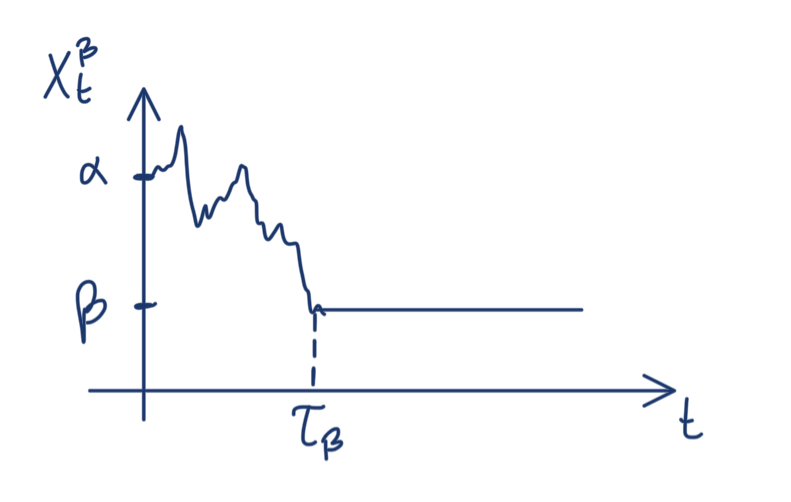
\includegraphics[width=0.5\textwidth]{images/barrier_above.jpeg}
\end{center}

\paragraph{$\alpha < \beta$: the process starts below the barrier.}

\begin{center}
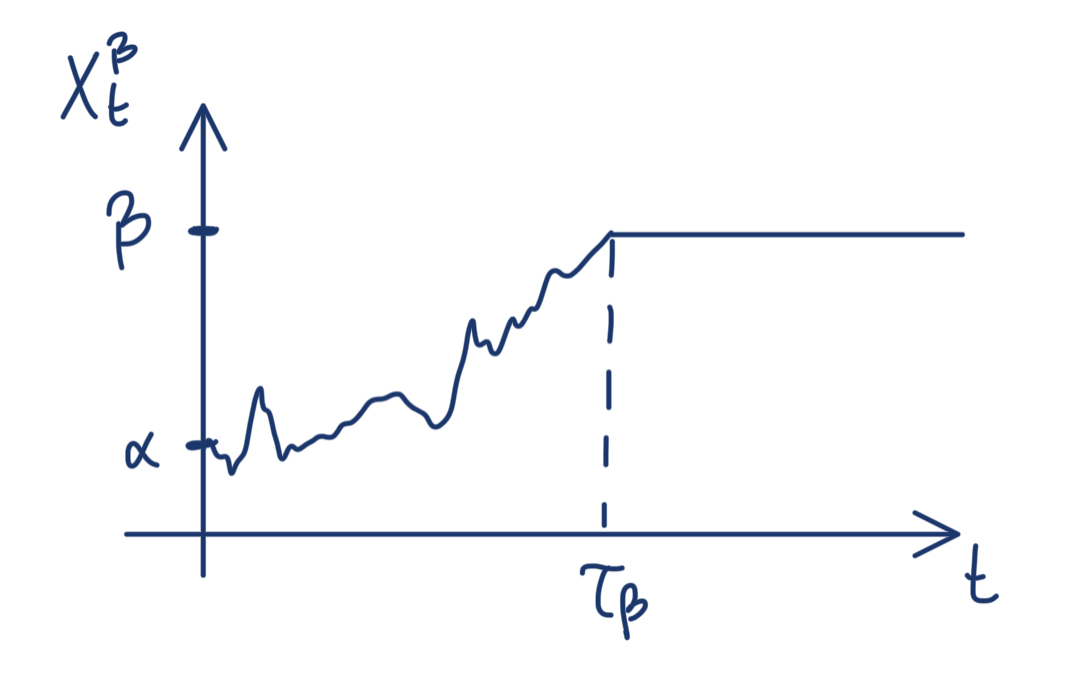
\includegraphics[width=0.5\textwidth]{images/barrier_below.jpeg}
\end{center}

\subsubsection{Distribution of the Stopped Process}

The random variable $X_t^\beta$ is \emph{mixed}:
\begin{itemize}
\item A point mass at the barrier $\beta$, because
\[
\mathbb{P}(X_t^\beta = \beta) > 0 \quad \forall\, t > 0.
\]
\item A continuous density on:
\begin{itemize}
\item $(\beta, +\infty)$ if $\alpha > \beta$, or
\item $(-\infty, \beta)$ if $\alpha < \beta$.
\end{itemize}
\end{itemize}

Hence the distribution combines:
\begin{itemize}
\item a Dirac mass at $\beta$,
\item a modified Gaussian density elsewhere.
\end{itemize}

\subsubsection{Density of $X_t^\beta$}

For all $x \in \mathbb{R}$, the density is:
\[
f_\beta(x; t, \alpha) = \varphi(x;\, \mu t + \alpha,\, \sigma\sqrt{t}) - \exp\!\left[-\frac{2\mu(\alpha - \beta)}{\sigma^2}\right]\, \varphi(x;\, \mu t - \alpha + 2\beta,\, \sigma\sqrt{t}),
\]
where
\[
\varphi(x; m, \gamma) = \frac{1}{\gamma\sqrt{2\pi}} \exp\!\left[-\frac{(x - m)^2}{2\gamma^2}\right]
\]
is the density of a normal random variable $N(m, \gamma^2)$.

\paragraph{Intuition:}

The second term is the ``reflected'' density (\emph{method of images}), correcting the probability so that the process is not allowed to cross the barrier.

\subsubsection{CDF of the Stopped Process}

We treat separately the cases $\alpha > \beta$ and $\alpha < \beta$.

\paragraph{Case 1: Initial value above the barrier ($\alpha > \beta$)}

\[
\mathbb{P}(X_t^\beta \leq x) = \begin{cases}
0, & x < \beta, \\
F_\beta(x; t, \alpha), & x \geq \beta,
\end{cases}
\]
where
\[
F_\beta(x; t, \alpha) = 1 - \int_x^{+\infty} f_\beta(y; t, \alpha)\, dy, \quad x \geq \beta.
\]

The CDF has a jump at $\beta$. The jump size is the probability mass at the barrier:
\[
\mathbb{P}(X_t^\beta = \beta) = 1 - \int_\beta^{+\infty} f_\beta(y; t, \alpha)\, dy > 0.
\]

\paragraph{Case 2: Initial value below the barrier ($\alpha < \beta$)}

\[
\mathbb{P}(X_t^\beta \leq x) = \begin{cases}
F_\beta(x; t, \alpha), & x < \beta, \\
1, & x \geq \beta.
\end{cases}
\]

Here:
\[
F_\beta(x; t, \alpha) = \int_{-\infty}^x f_\beta(y; t, \alpha)\, dy, \quad x < \beta.
\]

And the mass at the barrier is:
\[
\mathbb{P}(X_t^\beta = \beta) = 1 - \int_{-\infty}^\beta f_\beta(y; t, \alpha)\, dy.
\]

\subsubsection{Example: Brownian Motion with Drift = 0, Vol = 1, Barrier = 0}

Let:
\[
X_t = \alpha + W_t, \quad \beta = 0.
\]

We want the distribution of the process stopped at 0.

This is just a shifted Brownian motion, shifted up or down by $\alpha$.

\paragraph{Case $\alpha > 0$}

The probability of being absorbed is:
\[
\mathbb{P}(X_t^0 = 0) = 1 - \int_0^{+\infty} \big[\varphi(y; \alpha, \sqrt{t}) - \varphi(y; -\alpha, \sqrt{t})\big]\, dy.
\]

We now interpret the integrals as probabilities.

Since:
\begin{itemize}
\item $\varphi(y; \alpha, \sqrt{t})$ is the density of
\[
\alpha + \sqrt{t}\, Z \stackrel{d}{=} X_t, \quad Z \sim N(0, 1),
\]
\item $\varphi(y; -\alpha, \sqrt{t})$ is the density of
\[
-\alpha + \sqrt{t}\, Z,
\]
\end{itemize}
we have:
\[
\int_0^{+\infty} \varphi(y; \alpha, \sqrt{t})\, dy = \mathbb{P}(\alpha + \sqrt{t}\, Z > 0),
\]
\[
\int_0^{+\infty} \varphi(y; -\alpha, \sqrt{t})\, dy = \mathbb{P}(-\alpha + \sqrt{t}\, Z > 0).
\]

Then:
\[
\mathbb{P}(X_t^0 = 0) = 1 - \mathbb{P}(\alpha + \sqrt{t}\, Z > 0) + \mathbb{P}(-\alpha + \sqrt{t}\, Z > 0).
\]

Rewrite:
\[
\mathbb{P}(\alpha + \sqrt{t}\, Z \leq 0) = N\!\left(-\frac{\alpha}{\sqrt{t}}\right),
\]
\[
\mathbb{P}(-\alpha + \sqrt{t}\, Z \leq 0) = N\!\left(\frac{\alpha}{\sqrt{t}}\right).
\]

Thus:
\[
\mathbb{P}(X_t^0 = 0) = N\!\left(-\frac{\alpha}{\sqrt{t}}\right) + 1 - N\!\left(\frac{\alpha}{\sqrt{t}}\right) = 2\, N\!\left(-\frac{\alpha}{\sqrt{t}}\right) > 0.
\]

\paragraph{Case $\alpha < 0$}

Similarly we obtain:
\[
\mathbb{P}(X_t^0 = 0) = 2\, N\!\left(\frac{\alpha}{\sqrt{t}}\right).
\]

\subsection{Down-and-Out Contracts (D\&O Options)}

We consider the standard Black--Scholes market:
\[
\begin{cases}
dS_t = S_t(\alpha\, dt + \sigma\, dW_t), \\
dB_t = r B_t\, dt,
\end{cases}
\]
with initial condition $S_0 > L$, where $L \in \mathbb{R}$ is the barrier level.

In practice, the barrier may be defined as an absolute price level or as a percentage of the initial value.

We start with a ``simple'' contingent claim of the form:
\[
Z = \Phi(S_T),
\]
where $\Phi$ is the payoff function.

We denote by $F(t, s; \Phi)$ the pricing function of this claim.

This defines a family of pricing functions, one for each payoff $\Phi$.

\begin{definition}[Down-and-Out Option]
The \emph{down-and-out claim} associated with payoff $\Phi$ and barrier $L$ is denoted
\[
Z_{L,O}.
\]

\paragraph{Interpretation:}

\begin{itemize}
\item $L$ indicates the down barrier,
\item $O$ stands for \emph{out}, meaning the option becomes worthless if the price hits the barrier.
\end{itemize}
\end{definition}

\subsubsection{Contract Specification}

The option pays at maturity:
\[
Z_{L,O} = \begin{cases}
\Phi(S_T), & \text{if } S_t > L \text{ for all } t \in [0, T], \\
0, & \text{if } \exists\, t \in [0, T] \text{ such that } S_t \leq L.
\end{cases}
\]

Equivalently:
\[
Z_{L,O} = \Phi(S_T)\, \mathbbm{1}_{\{\inf_{t \in [0,T]} S_t > L\}}.
\]

\paragraph{Remark.}

On the event $\{\inf_{t \in [0,T]} S_t > L\}$, the process never touches the barrier.

Thus for all $t \in [0, T]$:
\[
S_t = S_t^L,
\]
where $S_t^L$ is the process stopped at the barrier $L$.

Hence:
\[
\Phi(S_T)\, \mathds{1}_{\{\inf_t S_t > L\}} = \Phi(S_T^L)\, \mathds{1}_{\{\inf_t S_t > L\}}.
\]

\subsubsection{Chopped Payoff}

Given any payoff function $\Phi$, define the \emph{chopped version}:
\[
\Phi_L(x) := \Phi(x)\, \mathds{1}_{\{x > L\}}.
\]

\paragraph{Remark.}

If $\inf_t S_t > L$, then:
\begin{itemize}
\item $S_t > L$ for all $t$,
\item equivalently $S_t^L > L$ for all $t$,
\end{itemize}
so the indicator of barrier survival is the same for $S$ and its stopped version:
\[
\mathds{1}_{\{\inf_t S_t > L\}} = \mathds{1}_{\{\inf_t S_t^L > L\}}.
\]

Thus:
\[
Z_{L,O} = \Phi(S_T^L)\, \mathds{1}_{\{\inf_t S_t^L > L\}} = \Phi_L(S_T^L).
\]

That is:

\emph{the down-and-out payoff equals the chopped payoff applied to the stopped process.}

\subsubsection{The Main Pricing Formula}

Define:
\[
\widetilde{r} := r - \frac{\sigma^2}{2}.
\]

\begin{theorem}
The no-arbitrage price of the down-and-out claim $Z_{L,O}$ is:
\[
\fbox{$F_{L,O}(t, s; \Phi) = F(t, s; \Phi_L) - \left(\frac{L}{s}\right)^{\frac{2\widetilde{r}}{\sigma^2}} F\!\left(t, \frac{L^2}{s}; \Phi_L\right)$}
\]
for all $t < T$ and initial price $s > L$.
\end{theorem}

\subsubsection{Proof Sketch (for $t = 0$)}

Assume $S_0 = s > L$.

Let $\tau_L = \inf\{t : S_t = L\}$ and $S_t^L = S_{t \wedge \tau_L}$.

From the risk--neutral valuation formula:
\[
F_{L,O}(0, s; \Phi) = e^{-rT}\, E_s^\mathbb{Q}[Z_{L,O}] = e^{-rT}\, E_s^\mathbb{Q}[\Phi_L(S_T^L)].
\]

\paragraph{Step 1: Express the dynamics under $\mathbb{Q}$}

Under $\mathbb{Q}$:
\[
S_t = e^{X_t}, \quad X_t = \ln s + \widetilde{r}\, t + \sigma W_t^\mathbb{Q}.
\]

Similarly:
\[
S_t^L = e^{X_t^{\ln L}},
\]
i.e.\ the log-price is stopped at level $\ln L$.

\paragraph{Step 2: Rewrite the expectation in log-coordinates}

\[
E_s^\mathbb{Q}[\Phi_L(S_T^L)] = \int_\mathbb{R} \Phi_L(e^x)\, f_{\ln L}(x; T, \ln s)\, \mathds{1}_{(\ln L, +\infty)}(x)\, dx.
\]

But since $\Phi_L(e^x) = 0$ whenever $e^x \leq L \iff x \leq \ln L$, the indicator is redundant:
\[
\Phi_L(e^x)\, \mathds{1}_{(\ln L, +\infty)}(x) = \Phi_L(e^x).
\]

Thus:
\[
E_s^\mathbb{Q}[Z_{L,O}] = \int_{\ln L}^{+\infty} \Phi_L(e^x)\, f_{\ln L}(x; T, \ln s)\, dx.
\]

\paragraph{Step 3: Reflection identity for the stopped log-normal density}

Using the reflection principle for Brownian motion and the explicit density of the stopped process, one obtains:
\[
f_{\ln L}(x; T, \ln s) = f(x; T, \ln s) - \left(\frac{L}{s}\right)^{\frac{2\widetilde{r}}{\sigma^2}} f\big(x; T, \ln(L^2/s)\big).
\]

Integrating against $\Phi_L(e^x)$ yields:
\[
E_s^\mathbb{Q}[Z_{L,O}] = E_s^\mathbb{Q}[\Phi_L(S_T)] - \left(\frac{L}{s}\right)^{\frac{2\widetilde{r}}{\sigma^2}} E_{L^2/s}^\mathbb{Q}[\Phi_L(S_T)].
\]

Multiplying by $e^{-rT}$ gives the pricing formula. \qed

\begin{corollary}[Linearity]
For any constants $\alpha, \beta$ and any contract functions $\Phi, \Psi$,
\[
F_{L,O}(t, s; \alpha\Phi + \beta\Psi) = \alpha\, F_{L,O}(t, s; \Phi) + \beta\, F_{L,O}(t, s; \Psi).
\]
\end{corollary}

This follows directly from linearity of expectation and of the pricing function $F$.

\subsection{Examples of D\&O Pricing Using Building Blocks}

We describe the standard building blocks and their pricing functions. These are the ingredients used to price more complex payoffs via linearity and the D\&O formula.

\subsubsection{Building Blocks (Payoffs)}

\begin{itemize}
\item \textbf{Bond payoff}
\[
BO(x) = 1
\]

\item \textbf{Stock payoff}
\[
ST(x) = x
\]

\item \textbf{Digital (``cash--or--nothing'') option}
\[
H(x; L) = \mathds{1}_{\{x > L\}}
\]

\item \textbf{Call option}
\[
C(x, K) = [x - K]^+
\]
\end{itemize}

\subsubsection{Pricing Functions (Vanilla Market)}

\begin{itemize}
\item \textbf{Bond}
\[
\overline{BO}(t, s) = e^{-r(T-t)}.
\]

\item \textbf{Stock}
\[
\overline{ST}(t, s) = s.
\]

\item \textbf{Digital option}
\[
\overline{H}(t, s; L) = e^{-r(T-t)}\, N\!\left(\frac{\ln(s/L) + \widetilde{r}(T-t)}{\sigma\sqrt{T-t}}\right), \quad \widetilde{r} := r - \frac{\sigma^2}{2}.
\]

\item \textbf{Call option}
\[
\overline{C}(t, s; K) = C_{BS}(t, s; K).
\]
\end{itemize}

\subsubsection{Example 1: Down-and-Out Bond}

The down-and-out payoff is:
\[
Z_{L,O} = \begin{cases}
1, & \inf_{0 \leq t \leq T} S_t > L, \\
0, & \text{otherwise}.
\end{cases}
= \mathds{1}_{\{\inf_t S_t > L\}}.
\]

Thus,
\[
\overline{BO}_{L,O}(t, s) = F_{L,O}(t, s; BO) = F(t, s; BO_L) - \left(\frac{L}{s}\right)^{\frac{2\widetilde{r}}{\sigma^2}} F\!\left(t, \frac{L^2}{s}; BO_L\right),
\]
where the chopped payoff is:
\[
BO_L(x) = BO(x)\, \mathds{1}_{\{x > L\}} = \mathds{1}_{\{x > L\}} = H(x; L).
\]

Thus:
\[
\overline{BO}_{L,O}(t, s) = \overline{H}(t, s; L) - \left(\frac{L}{s}\right)^{\frac{2\widetilde{r}}{\sigma^2}} \overline{H}\!\left(t, L^2/s; L\right).
\]

\subsubsection{Example 2: Down-and-Out Call}

The payoff is:
\[
Z_{L,O} = \begin{cases}
C(S_T; K), & \inf_t S_t > L, \\
0, & \text{otherwise}.
\end{cases}
\]

Hence,
\[
\overline{C}_{L,O}(t, s; K) = F_{L,O}(t, s; C) = F(t, s; C_L) - \left(\frac{L}{s}\right)^{\frac{2\widetilde{r}}{\sigma^2}} F\!\left(t, \frac{L^2}{s}; C_L\right),
\]
where $C_L$ is the chopped version:
\[
C_L(x; K) := C(x; K)\, \mathds{1}_{\{x > L\}}.
\]

We analyse two cases.

\paragraph{Case 1: $L \leq K$}

Here the call is already zero on the interval $[L, K]$.

Thus chopping at $L$ does not change the payoff:
\[
C_L(s; K) = C(s; K).
\]

Hence:
\[
\overline{C}_{L,O}(t, s; K) = C_{BS}(t, s; K) - \left(\frac{L}{s}\right)^{\frac{2\widetilde{r}}{\sigma^2}} C_{BS}\!\left(t, \frac{L^2}{s}; K\right)
\]

\paragraph{Case 2: $L > K$}

In this case the payoff of the call is:
\begin{itemize}
\item zero for $s \leq K$,
\item positive for $s > K$,
\end{itemize}
but chopping at $L$ kills the payoff on the interval $[K, L]$.

The chopped payoff is:
\begin{itemize}
  \item zero on $(-\infty, L]$,
  \item equal to $[s - K]^+$ for $s > L$.
\end{itemize}

We can rewrite this as:
\[
C_L(s; K) = C(s; L) + (L - K)\, H(s; L).
\]

\paragraph{Intuition:}

A call with strike $K$ but forced to be zero until $L$ is:
\begin{itemize}
\item a call struck at $L$,
\item plus a jump of size $L - K$ if $s > L$, i.e.\ a digital option.
\end{itemize}

Using linearity of pricing:
\[
\overline{C}_L(t, s; K) = C_{BS}(t, s; L) + (L - K)\, \overline{H}(t, s; L).
\]

Then:
\[
\begin{aligned}
\overline{C}_{L,O}(t, s; K) &= C_{BS}(t, s; L) - \left(\frac{L}{s}\right)^{\frac{2\widetilde{r}}{\sigma^2}} C_{BS}\!\left(t, \frac{L^2}{s}; L\right) \\
&\quad + (L - K)\, \overline{H}(t, s; L) - (L - K)\left(\frac{L}{s}\right)^{\frac{2\widetilde{r}}{\sigma^2}} \overline{H}\!\left(t, \frac{L^2}{s}; L\right).
\end{aligned}
\]

\subsubsection{Put-Call Parity for Down-and-Out Contracts}

Recall vanilla parity:
\[
P(x; K) = K\, BO(x) - ST(x) + C(x; K).
\]

By linearity of pricing and of the D\&O operator $F_{L,O}$, we get:
\[
\overline{P}_{L,O}(t, s; K) = K\, \overline{BO}_{L,O}(t, s) - \overline{ST}_{L,O}(t, s) + \overline{C}_{L,O}(t, s; K).
\]

\newpage
\section{November 20, 2025}

\subsection{Down \& Out Put-Call Parity}

We start by defining the Put-Call Parity specifically for a Down \& Out barrier option.

The relationship is given by:
\[
\underline{P}_{L,O}(t, s; K) = K\, \underline{BO}_{L,O}(t, s) - \underline{ST}_{L,O}(t, s) + \underline{C}_{L,O}(t, s; K).
\]

\paragraph{Breakdown of terms:}
\begin{itemize}
\item $\underline{P}_{L,O}$: Price of a Down \& Out Put.
\item $K\, \underline{BO}_{L,O}$: The strike price discounted, multiplied by the price of a Down \& Out Bond (a binary option that pays 1 if the barrier is not breached).
\item $\underline{ST}_{L,O}$: Price of a Down \& Out Asset (or Stock) contract.
\item $\underline{C}_{L,O}$: Price of a Down \& Out Call.
\end{itemize}

\subsection{Up \& Out Contract}

Let's define a contingent claim $Z = \Phi(S_T)$. We now consider an \textbf{Up \& Out (U\&O)} contract.

\begin{definition}[Up \& Out Contract]
The payoff $Z_{L,O}$ for an Up \& Out contract is defined as:
\begin{itemize}
\item If $\forall t \in [0,T],\, S_t < L \quad \Longrightarrow$ At time $T$, the holder receives the payoff $Z$.
\item If $\exists t \in [0,T],\, S_t \geq L \quad \Longrightarrow$ The contract becomes null \& void (knocks out), and the holder gets $0$.
\end{itemize}
\end{definition}

\begin{remark}
Here, $L$ is the upper barrier. The contract survives only if the asset price stays below $L$.
\end{remark}

\paragraph{Payoff Formulation}

At $t=0$, we assume $S_0 < L$, where $L \in \mathbb{R}$. We can write the payoff $Z_{L,O}$ mathematically as:
\[
Z_{L,O} = 
\begin{cases}
\Phi(S_T), & \text{if } \sup_{t \in [0,T]} S_t < L, \\
0, & \text{otherwise}
\end{cases}
= \Phi(S_T) \cdot \mathds{1}_{\{\sup S_t < L\}}.
\]

\paragraph{The "Chopped" Payoff}

To handle this mathematically, we introduce the concept of the \emph{chopped} (or truncated) payoff, denoted as $\Phi_L$:
\[
\Phi_L(X) = \Phi(X)\, \mathds{1}_{\{X < L\}}.
\]

\textbf{Logical Step:} On the event $\{\sup_t S_t < L\}$, it implies that the asset price never touched $L$. Therefore, the final price $S_T$ must also be strictly less than $L$.
\[
S_t < L\, \forall t \quad \Longleftrightarrow \quad S_t^L < L\, \forall t,
\]
where $S^L$ denotes the process restricted by the barrier.

Thus, we can rewrite the payoff indicator:
\[
\Phi(S_T)\, \mathds{1}_{\{\sup_t S_t < L\}} = \Phi(S_T)\, \mathds{1}_{\{S_T^L < L\}} = \Phi(S_T^L)\, \mathds{1}_{\{S_T^L < L\}} = \Phi_L(S_T^L).
\]

\begin{theorem}[Pricing the Up \& Out Contract]
Let $\widetilde{r} := r - \sigma^2/2$. The No-Arbitrage (NA) price at time $t$ of the claim $Z_{L,O}$ is given by the Reflection Principle result:
\[
F_{L,O}(t, s; \Phi_L) = F(t, s; \Phi_L) - \left(\frac{s}{L}\right)^{\frac{2\widetilde{r}}{\sigma^2}} F\!\left(t, \frac{L^2}{s}; \Phi_L\right).
\]
\end{theorem}

\subsection{In Contracts (In \& Out Parity)}

Now we look at \textbf{Knock-In} contracts. Let the vanilla claim be $Z = \Phi(S_T)$.

\subsubsection{Definitions}

\begin{definition}[Down \& In (D\&I) Contract]
\[
Z_{L,I} = 
\begin{cases}
0, & \text{if } S_t > L\, \text{(Barrier never hit)}, \\
\Phi(S_T), & \text{otherwise (Barrier hit)}.
\end{cases}
\]
\end{definition}

\begin{remark}
The contract activates only if the price drops to touch $L$.
\end{remark}

\begin{definition}[Up \& In (U\&I) Contract]
\[
Z_{L,I} = 
\begin{cases}
0, & \text{if } S_t < L, \\
\Phi(S_T), & \text{otherwise}.
\end{cases}
\]
\end{definition}

\begin{remark}
The contract activates only if the price rises to touch $L$.
\end{remark}

\subsubsection{In \& Out Parity}

A fundamental relationship exists between "In" and "Out" options. If you hold both an "In" option and an "Out" option with the same barrier, you are guaranteed the payoff $\Phi(S_T)$ regardless of whether the barrier is hit or not.

\begin{proposition}[In \& Out Parity]
\[
Z_{L,I} + Z_{L,O} = \Phi(S_T) = Z.
\]
This implies for the prices:
\[
F_{L,I}(t, s; \Phi) = F(t, s; \Phi) - F_{L,O}(t, s; \Phi).
\]
\end{proposition}

\subsection{Pricing Derivation for Up \& In (U\&I)}

Using the parity relation and the Up \& Out theorem derived earlier:
\[
\begin{aligned}
F_{L,I}(t, s; \Phi) &= F(t, s; \Phi) - F_{L,O}(t, s; \Phi) \\
&= F(t, s; \Phi) - \left[F(t, s; \Phi_L) - \left(\frac{s}{L}\right)^{\frac{2\widetilde{r}}{\sigma^2}} F\!\left(t, \frac{L^2}{s}; \Phi_L\right)\right].
\end{aligned}
\]

\textbf{Logical Step:} We can decompose the general payoff $\Phi$ into the part below the barrier and the part above the barrier:
\[
\Phi = \Phi_L + \Phi^L,
\]
where $\Phi_L$ is the payoff truncated at $L$, and $\Phi^L$ is the payoff "starting" from $L$.

Substituting this into the equation ($F(t, s; \Phi) = F(t, s; \Phi_L) + F(t, s; \Phi^L)$):
\[
\begin{aligned}
F_{L,I}(t, s; \Phi) &= F(t, s; \Phi^L) + F(t, s; \Phi_L) - F(t, s; \Phi_L) + \left(\frac{s}{L}\right)^{\frac{2\widetilde{r}}{\sigma^2}} F\!\left(t, \frac{L^2}{s}; \Phi_L\right).
\end{aligned}
\]

Simplifying (the $F(t, s; \Phi_L)$ terms cancel out):
\[
F_{L,I}(t, s; \Phi) = F(t, s; \Phi^L) + \left(\frac{s}{L}\right)^{\frac{2\widetilde{r}}{\sigma^2}} F\!\left(t, \frac{L^2}{s}; \Phi_L\right).
\]

\subsection{Pricing Down \& In}

\paragraph{Derivation:} We now write the same derivation for the Down \& In ($F_{L,I}$) contract.

We start with the In-Out Parity:
\[
F_{L,I}(t, s; \Phi) = F(t, s; \Phi) - F_{L,O}(t, s; \Phi).
\]

For a Down \& Out contract (where barrier $L < S_0$), the pricing theorem (symmetric to the Up \& Out case) involves the payoff truncated above $L$ (denoted $\Phi^L$). The Down \& Out price is:
\[
F_{L,O}(t, s; \Phi) = F(t, s; \Phi^L) - \left(\frac{L}{s}\right)^{\frac{2\widetilde{r}}{\sigma^2}} F\!\left(t, \frac{L^2}{s}; \Phi^L\right).
\]

Now substitute this into the parity equation:
\[
F_{L,I}(t, s; \Phi) = F(t, s; \Phi) - \left[F(t, s; \Phi^L) - \left(\frac{L}{s}\right)^{\frac{2\widetilde{r}}{\sigma^2}} F\!\left(t, \frac{L^2}{s}; \Phi^L\right)\right].
\]

Decompose the vanilla payoff $\Phi = \Phi^L + \Phi_L$:
\[
\begin{aligned}
F_{L,I}(t, s; \Phi) &= \left[F(t, s; \Phi^L) + F(t, s; \Phi_L)\right] - F(t, s; \Phi^L) + \left(\frac{L}{s}\right)^{\frac{2\widetilde{r}}{\sigma^2}} F\!\left(t, \frac{L^2}{s}; \Phi^L\right).
\end{aligned}
\]

\paragraph{Final Result for Down \& In:}
\[
F_{L,I}(t, s; \Phi) = F(t, s; \Phi_L) + \left(\frac{L}{s}\right)^{\frac{2\widetilde{r}}{\sigma^2}} F\!\left(t, \frac{L^2}{s}; \Phi^L\right).
\]

\subsection{PDE for Barrier Options}

We can also price barrier options by solving the Partial Differential Equation (PDE) directly.

\subsubsection{Standard Black-Scholes PDE}

The framework starts with the standard equation:
\[
\begin{cases}
F_t + rs F_s + \frac{\sigma^2}{2} s^2 F_{ss} - rF = 0, \\
F(T, s) = \Phi(s).
\end{cases}
\]

\paragraph{Boundary Conditions for Numerical Solution:}

For a standard Call option:
\begin{itemize}
\item $F(t, 0) = 0$ (If stock is 0, call is worth 0)
\item $F(t, s) \to s$ as $s \to +\infty$
\end{itemize}

\subsubsection{Adjusting for Barrier Options}

For a Down \& Out (D\&O) Call option with barrier $L$:
\begin{itemize}
\item The option becomes worthless if $S$ touches $L$.
\item \textbf{New Boundary Condition:} We specify $F(t, L) = 0$ instead of $F(t, 0) = 0$.
\item \textbf{New Domain:} The PDE holds in $[0, T] \times [L, +\infty)$.
\end{itemize}

\subsubsection{Transformation to Heat Equation}

To solve this analytically, we transform the Black-Scholes PDE into the Heat Equation. The standard Heat Equation problem is:
\[
\begin{cases}
u_\tau - u_{xx} = 0, \\
\lim_{x \to \pm\infty} u(\tau, x) = 0, \\
u(0, x) = \left[e^{\frac{k+1}{2}x} - e^{\frac{k-1}{2}x}\right]^+.
\end{cases}
\]

\paragraph{The Barrier Modification:}

Because our domain is restricted by the barrier $L$, we must adjust the spatial boundary condition. We substitute the $-\infty$ limit with a boundary condition at a specific point $x_0$, which corresponds to the barrier level in log-coordinates.

\begin{itemize}
\item Define $x_0 = \ln(L/K)$.
\item The new condition is: $u(\tau, x_0) = 0$.
\item The new domain will be $[0, T] \times [x_0, +\infty)$.
\end{itemize}

This setup allows us to use the \textbf{Method of Images} (reflection principle) to find the solution $u(\tau, x)$, which we then transform back to get the option price $F(t, s)$.

\subsection{Lookback Options}

A \textbf{lookback option} is a path-dependent option whose payoff depends on the running maximum or running minimum of the underlying price process $(S_t)_{t \in [0,T]}$.

For a generic process $X = (X_t)_{t \geq 0}$, define:

\paragraph{Running maximum}
\[
M_t^X := \sup_{u \in [0,t]} X_u.
\]

\paragraph{Running minimum}
\[
m_t^X := \inf_{u \in [0,t]} X_u.
\]

When $X_t = S_t$, we simply write $M_t^S, m_t^S$.

\subsubsection{Types of Lookback Options}

\paragraph{1. Floating-strike lookback options}

\textbf{Lookback call}
\[
Z = [S_T - m_T^S]^+.
\]
However, since
\[
S_T \geq m_T^S \quad \Longrightarrow \quad [S_T - m_T^S]^+ = S_T - m_T^S,
\]
the payoff is usually written as:
\[
Z = S_T - m_T^S.
\]

\textbf{Lookback put}
\[
Z = [M_T^S - S_T]^+.
\]
Similarly, we always have $M_T^S \geq S_T$, hence:
\[
Z = M_T^S - S_T.
\]

So in the floating case the strike is effectively the best (minimum or maximum) price attained by the underlying over $[0,T]$.

\paragraph{2. Fixed-strike (forward) lookback options}

Let $K$ be a fixed strike.

\textbf{Forward lookback call}
\[
Z = [M_T^S - K]^+.
\]

\textbf{Forward lookback put}
\[
Z = [K - m_T^S]^+.
\]

Here the payoff compares the fixed strike $K$ with the extreme value of the underlying over the life of the option.

\subsubsection{Distribution of the Running Maximum of a Brownian Motion with Drift}

Let
\[
X_t = \alpha + \mu t + \sigma W_t, \quad t \geq 0,
\]
where $W$ is a standard Brownian motion, and define
\[
M_t^X := \sup_{0 \leq u \leq t} X_u.
\]

\begin{proposition}
The cdf of $M_t^X$ is given by
\[
F_{M_t^X}(x) = 
\begin{cases}
\text{(this case will be discussed later)}, & x < \alpha, \\[6pt]
\Phi\!\left(\frac{x - \alpha - \mu t}{\sigma\sqrt{t}}\right) - \exp\!\left(\frac{2\mu(x - \alpha)}{\sigma^2}\right) \Phi\!\left(\frac{x - \alpha + \mu t}{\sigma\sqrt{t}}\right), & x \geq \alpha,
\end{cases}
\]
where $\Phi$ is the standard normal cdf.
\end{proposition}

\begin{remark}
In your notes the $t$ vs $T$ notation is a bit mixed; conceptually, this is the standard reflection principle formula for the running maximum of a Brownian motion with drift.
\end{remark}

\subsubsection{Pricing a Floating-Strike Lookback Put in Black-Scholes}

We want the no-arbitrage price at time $0$ of a floating-strike lookback put:
\[
Z = M_T^S - S_T,
\]
in the Black-Scholes model (no dividends).

\paragraph{Risk-neutral dynamics}

Under the risk-neutral measure $\mathbb{Q}$:
\[
\begin{cases}
dS_t = S_t\, (r\, dt + \sigma\, dW_t^{\mathbb{Q}}), \\
S_0 = s.
\end{cases}
\]

Define the \textbf{log-price process}
\[
X_t := \ln S_t.
\]

By Itô, we have
\[
X_t = \ln s + \widetilde{r}\, t + \sigma W_t^{\mathbb{Q}},
\]
where
\[
\widetilde{r} := r - \frac{\sigma^2}{2}.
\]

So we are exactly in the setting $X_t = \alpha + \mu t + \sigma W_t$ with:
\[
\alpha = \ln s, \quad \mu = \widetilde{r}, \quad \sigma = \sigma.
\]

\paragraph{Price via risk-neutral valuation}

The time-0 price is
\[
\begin{aligned}
\Pi_0 &= \Pi_0(M_T^S - S_T) = \mathbb{E}_{0,s}^{\mathbb{Q}}\left[e^{-rT}(M_T^S - S_T)\right] \\
&= e^{-rT}\, \mathbb{E}_{0,s}^{\mathbb{Q}}[M_T^S] - e^{-rT}\, \mathbb{E}_{0,s}^{\mathbb{Q}}[S_T].
\end{aligned}
\]

Under $\mathbb{Q}$, $\mathbb{E}[S_T] = s e^{rT}$, hence:
\[
e^{-rT} \mathbb{E}_{0,s}^{\mathbb{Q}}[S_T] = s.
\]

Thus
\[
\Pi_0 = e^{-rT}\, \mathbb{E}_{0,s}^{\mathbb{Q}}[M_T^S] - s.
\]

So the "interesting" part is $\mathbb{E}[M_T^S]$.

\paragraph{Expressing $M_T^S$ via the running maximum of $X_t$}

Since $S_t = e^{X_t}$ and the exponential function is strictly increasing, we have:
\[
M_T^S = \sup_{0 \leq u \leq T} S_u = \sup_{0 \leq u \leq T} e^{X_u} = e^{M_T^X},
\]
where
\[
M_T^X = \sup_{0 \leq u \leq T} X_u.
\]

Therefore:
\[
\mathbb{E}_{0,s}^{\mathbb{Q}}[M_T^S] = \mathbb{E}_{0,s}^{\mathbb{Q}}[e^{M_T^X}].
\]

\paragraph{Computing $\mathbb{E}[e^{M_T^X}]$}

From the cdf $F_{M_T^X}$ above, we can obtain the density $f_{M_T^X}(x)$ by differentiating. This density naturally splits into two parts, which leads to a decomposition of the expectation into two integrals.

For $x \geq \ln s$, differentiating
\[
F_{M_T^X}(x) = \Phi\!\left(\frac{x - \ln s - \widetilde{r}\, T}{\sigma\sqrt{T}}\right) - \exp\!\left(\frac{2\widetilde{r}(x - \ln s)}{\sigma^2}\right) \Phi\!\left(\frac{x - \ln s + \widetilde{r}\, T}{\sigma\sqrt{T}}\right)
\]
yields (schematically)
\[
f_{M_T^X}(x) = \frac{1}{\sigma\sqrt{T}}\, \varphi\!\left(\frac{x - \ln s - \widetilde{r}\, T}{\sigma\sqrt{T}}\right) - \text{(derivative of the second term)}.
\]

Therefore:
\[
\mathbb{E}_{0,s}^{\mathbb{Q}}[e^{M_T^X}] = \int_{\ln s}^{+\infty} e^x f_{M_T^X}(x)\, dx = I_1 + I_2,
\]
with:
\[
I_1 := \int_{\ln s}^{+\infty} e^x\, \frac{1}{\sigma\sqrt{T}}\, \varphi\!\left(\frac{x - \ln s - \widetilde{r}\, T}{\sigma\sqrt{T}}\right) dx,
\]
\[
I_2 := -\int_{\ln s}^{+\infty} e^x\, d\left[\exp\!\left(\frac{2\widetilde{r}(x - \ln s)}{\sigma^2}\right) \Phi\!\left(-\frac{x - \ln s + \widetilde{r}\, T}{\sigma\sqrt{T}}\right)\right].
\]

Here $\varphi$ is the standard normal pdf.

\begin{remark}
Your note: "Where we found that by differentiating $F_{M_T^X}(x)$" refers exactly to this decomposition.
\end{remark}

\paragraph{Computation of $I_1$}

Start from:
\[
I_1 = \int_{\ln s}^{+\infty} \frac{1}{\sigma\sqrt{T}}\, \frac{1}{\sqrt{2\pi}}\, \exp\!\left(x - \frac{1}{2}\left(\frac{x - \ln s - \widetilde{r}\, T}{\sigma\sqrt{T}}\right)^2\right) dx.
\]

Introduce the change of variable:
\[
y := \frac{x - \ln s - \widetilde{r}\, T}{\sigma\sqrt{T}} \quad \Longrightarrow \quad dy = \frac{1}{\sigma\sqrt{T}}\, dx,
\]
so
\[
x = \ln s + \widetilde{r}\, T + \sigma\sqrt{T}\, y.
\]

As $x$ ranges from $\ln s$ to $+\infty$,
\begin{itemize}
\item when $x = \ln s$:
\[
y = \frac{\ln s - \ln s - \widetilde{r}\, T}{\sigma\sqrt{T}} = -\frac{\widetilde{r}\sqrt{T}}{\sigma},
\]
\item when $x \to +\infty$: $y \to +\infty$.
\end{itemize}

Thus:
\[
\begin{aligned}
I_1 &= \int_{-\frac{\widetilde{r}\sqrt{T}}{\sigma}}^{+\infty} \frac{1}{\sqrt{2\pi}}\, \exp\left((\ln s + \widetilde{r}\, T + \sigma\sqrt{T}\, y) - \frac{1}{2}y^2\right) dy \\
&= s\, e^{\widetilde{r}\, T} \int_{-\frac{\widetilde{r}\sqrt{T}}{\sigma}}^{+\infty} \frac{1}{\sqrt{2\pi}}\, \exp\left(\sigma\sqrt{T}\, y - \frac{1}{2}y^2\right) dy.
\end{aligned}
\]

Complete the square inside the exponential:
\[
\sigma\sqrt{T}\, y - \frac{1}{2}y^2 = -\frac{1}{2}(y^2 - 2\sigma\sqrt{T}\, y) = -\frac{1}{2}(y - \sigma\sqrt{T})^2 + \frac{1}{2}\sigma^2 T.
\]

Therefore:
\[
\begin{aligned}
I_1 &= s\, e^{\widetilde{r}\, T} \int_{-\frac{\widetilde{r}\sqrt{T}}{\sigma}}^{+\infty} \frac{1}{\sqrt{2\pi}}\, \exp\left(-\frac{1}{2}(y - \sigma\sqrt{T})^2\right)\, e^{\frac{\sigma^2 T}{2}}\, dy \\
&= s\, e^{\widetilde{r}\, T}\, e^{\frac{\sigma^2 T}{2}} \int_{-\frac{\widetilde{r}\sqrt{T}}{\sigma}}^{+\infty} \frac{1}{\sqrt{2\pi}}\, \exp\left(-\frac{1}{2}(y - \sigma\sqrt{T})^2\right) dy.
\end{aligned}
\]

Since $\widetilde{r} = r - \frac{\sigma^2}{2}$, we have
\[
e^{\widetilde{r}\, T}\, e^{\frac{\sigma^2 T}{2}} = e^{rT},
\]
so:
\[
I_1 = s\, e^{rT} \int_{-\frac{\widetilde{r}\sqrt{T}}{\sigma}}^{+\infty} \frac{1}{\sqrt{2\pi}}\, \exp\left(-\frac{1}{2}(y - \sigma\sqrt{T})^2\right) dy.
\]

Now, the integral is the probability of a Gaussian with mean $\sigma\sqrt{T}$ and variance $1$:
\[
\int_{-\frac{\widetilde{r}\sqrt{T}}{\sigma}}^{+\infty} \frac{1}{\sqrt{2\pi}}\, \exp\left(-\frac{1}{2}(y - \sigma\sqrt{T})^2\right) dy = \mathbb{P}\left(\sigma\sqrt{T} + Z \geq -\frac{\widetilde{r}\sqrt{T}}{\sigma}\right),
\]
where $Z \sim N(0,1)$.

Equivalently:
\[
\mathbb{P}\left(Z \geq -\frac{\widetilde{r}\sqrt{T}}{\sigma} - \sigma\sqrt{T}\right) = \Phi(d),
\]
for a suitable
\[
d = \frac{rT + \frac{1}{2}\sigma^2 T}{\sigma\sqrt{T}}
\]
(as in your notes, after simplification).

So finally:
\[
I_1 = s e^{rT} \Phi(d).
\]

\begin{remark}
That matches your final sentence: "We can interpret this integral as $s e^{rT} \mathbb{P}(\sigma\sqrt{T} + Z \geq -\frac{\widetilde{r}\sqrt{T}}{\sigma}) = s e^{rT} \mathbb{P}(Z \geq -\frac{\widetilde{r}\sqrt{T}}{\sigma} - \sigma\sqrt{T}) = s e^{rT} N(d)$."
\end{remark}

\paragraph{$I_2$ and final price formula}

The second term $I_2$ is obtained by integrating by parts:
\[
I_2 = -\int_{\ln s}^{+\infty} e^x\, d\left[\exp\!\left(\frac{2\widetilde{r}(x - \ln s)}{\sigma^2}\right) \Phi\!\left(-\frac{x - \ln s + \widetilde{r}\, T}{\sigma\sqrt{T}}\right)\right].
\]

Carrying out this computation (standard but more tedious), and combining it with the result for $I_1$, one finally obtains:
\[
\mathbb{E}_{0,s}^{\mathbb{Q}}[M_T^S] = s\left[\frac{\sigma}{2r}\, \Phi(d) - \Phi(-d)\right] + s e^{rT}\, \Phi(-d + \sigma\sqrt{T})\left(\frac{\sigma^2}{2r} - 1\right),
\]
and hence the no-arbitrage price at time 0 of the floating-strike lookback put is:
\[
\boxed{
\Pi_0(M_T^S - S_T) = s\left[\frac{\sigma}{2r}\, \Phi(d) - \Phi(-d)\right] - s e^{-rT}\, \Phi(-d + \sigma\sqrt{T})\left(\frac{\sigma^2}{2r} - 1\right),
}
\]
with
\[
d = \frac{rT + \frac{1}{2}\sigma^2 T}{\sigma\sqrt{T}}.
\]

\subsection{Asian Options}

An \textbf{Asian option} is a path-dependent derivative whose payoff depends on some average of the underlying price process $(S_t)_{t \in [0,T]}$.

Two types of averages are commonly used.

\subsubsection{Definitions of Averages}

\paragraph{Arithmetic average}
\[
A_t := \frac{1}{T} \int_0^t S_u\, du.
\]

\paragraph{Geometric average}
\[
\Gamma_t := \exp\!\left(\frac{1}{T} \int_0^t \ln S_u\, du\right).
\]

Both aggregates are path-dependent quantities but become state variables once incorporated into the pricing PDE.

\subsubsection{Examples of Asian Option Payoffs}

\paragraph{Fixed-strike (average rate) options}

\textbf{Asian call}
\[
Y = [A_T - K]^+, \quad \text{or} \quad Y = [\Gamma_T - K]^+.
\]

\paragraph{Floating-strike (average strike) options}

\textbf{Asian call}
\[
Y = [S_T - A_T]^+, \quad \text{or} \quad Y = [S_T - \Gamma_T]^+.
\]

\subsubsection{Structure of the Pricing Problem}

Take for example the arithmetic fixed-strike Asian call:
\[
Y = [A_T - K]^+.
\]

Since
\[
A_T = \frac{1}{T} \int_0^T S_u\, du,
\]
the payoff can be written as a function of time, terminal spot, and the accumulated integral:
\[
Y = \Phi(T, S_T, A_T).
\]

Thus the pricing function must depend on both variables $(S_t, A_t)$. We need a PDE in two spatial variables.

\subsubsection{Adding an Auxiliary State Variable}

Introduce the running integral:
\[
Z_t := \int_0^t g(S_u)\, du,
\]
where $g$ is any measurable function depending on the desired average.

\paragraph{Examples:}

\begin{itemize}
\item \textbf{Arithmetic average:}
\[
A_T = \frac{1}{T} Z_T, \quad g(s) = s.
\]

\item \textbf{Geometric average:}
\[
\Gamma_T = \exp\!\left(\frac{1}{T} Z_T\right), \quad g(s) = \ln s.
\]
\end{itemize}

The price can then be expressed as:
\[
\Pi_t(Y) = F(t, S_t, Z_t).
\]

\subsubsection{Dynamics under the Risk-Neutral Measure}

Under $\mathbb{Q}$:
\[
\begin{cases}
dB_t = r B_t\, dt, \\
dS_t = S_t\, (r\, dt + \sigma\, dW_t^{\mathbb{Q}}), \\
dZ_t = g(S_t)\, dt.
\end{cases}
\]

\paragraph{Note:}
\begin{itemize}
\item The new state variable $Z_t$ has no diffusion term.
\item It is unaffected by the Girsanov transformation.
\item The augmented process $(S_t, Z_t)$ is Markov, so pricing reduces to solving a PDE in $(t, s, z)$.
\end{itemize}

\subsubsection{Pricing PDE for Asian Options}

If $F(t, s, z)$ is the price function, and assuming $F \in C^{1,2}$, Itô's formula applied to $F(t, S_t, Z_t)$ and the martingale property of discounted prices gives:
\[
\boxed{
F_t + rs F_s + \frac{\sigma^2}{2} s^2 F_{ss} + g(s)\, F_z - rF = 0
}
\]
with terminal condition:
\[
F(T, s, z) = \Phi(T, s, z).
\]

This PDE must be solved on the domain:
\[
(t, s, z) \in [0, T] \times \mathbb{R}_+ \times \mathbb{R}.
\]

\newpage
\section{November 24, 2025}

\subsection{Introducing the Auxiliary Process $Z_t$}

Define
\[
Z_t = \int_0^t g(S_u)\, du.
\]

This variable accumulates some function of the past prices.

\paragraph{Typical examples:}
\begin{itemize}
\item \textbf{geometric average:} $g(s) = \ln s$
\item \textbf{arithmetic average:} $g(s) = s$
\end{itemize}

Once we augment the state vector to $(B_t, S_t, Z_t)$, the pricing problem becomes Markovian again.

Thus, the arbitrage-free (risk-neutral) price of a derivative with payoff $\Phi(T, S_T, Z_T)$ is
\[
F(t, s, z) = \mathbb{E}_{t,s,z}^{\mathbb{Q}}\left[e^{-r(T-t)} \Phi(T, S_T, Z_T)\right].
\]

If we do not include $Z_t$, the pricing problem cannot be expressed in a Markovian form.

\subsection{PDE for Asian Options (Markovian Representation)}

Assume sufficient smoothness:
\[
F \in C^{1,2,1}([0, T] \times \mathbb{R}_+ \times \mathbb{R}_+).
\]

Under the risk-neutral dynamics $dS_t = r S_t\, dt + \sigma S_t\, dW_t^{\mathbb{Q}}$, and by applying Itô's formula to $F(t, S_t, Z_t)$, we obtain the pricing PDE:
\[
\boxed{
F_t + rs F_s + \frac{1}{2}\sigma^2 s^2 F_{ss} + g(s) F_z - rF = 0
}
\]
with terminal condition
\[
F(T, s, z) = \Phi(T, s, z), \quad (s, z) \in \mathbb{R}_+^2.
\]

This yields a semi-explicit pricing representation.

\begin{remark}
Not all path-dependent options admit such a reduction—e.g. lookback options remain non-Markovian in any finite dimension.
\end{remark}

\subsection{Example: Geometric Average Price Asian Call/Put}

Consider the payoff
\[
\Phi(S_T, Z_T) = \left[\exp\!\left(\frac{1}{T} Z_T\right) - K\right]^+ \quad \text{with } g(s) = \ln s.
\]

Thus
\[
Z_T = \int_0^T \ln(S_u)\, du, \quad \Phi = \left[\exp\!\left(\frac{1}{T} \int_0^T \ln(S_u)\, du\right) - K\right]^+.
\]

Define the time-averaged log-price:
\[
\overline{X}_T := \frac{Z_T}{T} = \frac{1}{T} \int_0^T X_u\, du, \quad X_t = \ln(S_t).
\]

Under $\mathbb{Q}$,
\[
X_t = \ln s + \widetilde{r}\, t + \sigma W_t^{\mathbb{Q}}, \quad \widetilde{r} := r - \frac{\sigma^2}{2}.
\]

Thus the payoff simplifies to
\[
\Phi = [e^{\overline{X}_T} - K]^+.
\]

\paragraph{Is $\overline{X}_T$ Gaussian?}

Yes. $\overline{X}_T$ is a linear functional of a Gaussian process, hence Gaussian.

A standard computation using Itô's formula (or direct integration of a Brownian motion) gives:
\[
\overline{X}_T \sim N\!\left(\left(r - \frac{\sigma^2}{2}\right)\frac{T}{2},\, \frac{\sigma^2 T}{3}\right)
\]

Consequently,
\[
e^{\overline{X}_T} \sim \log N\!\left(\left(r - \frac{\sigma^2}{2}\right)\frac{T}{2},\, \frac{\sigma^2 T}{3}\right).
\]

Thus the price can be computed by plugging these parameters into the Black-Scholes formula for a lognormal underlying.

\paragraph{Asian geometric-average price call}
\[
C_{AGB}(0, s) = s\, \exp\!\left\{-\frac{1}{2}\left(r - \sigma^2/2\right)T\right\} N(d_1) - K e^{-rT} N(d_2),
\]
where
\[
d_1 = \frac{\ln(s/K) + \frac{1}{2}\left(r - \frac{\sigma^2}{6}\right)T}{\sigma\sqrt{T/3}}, \quad d_2 = d_1 - \sigma\sqrt{T/3}.
\]

\subsection{Example: Arithmetic Average-Strike Asian Call}

\paragraph{Payoff:}
\[
\Phi(T, S_T, Z_T) = [S_T - Z_T/T]^+.
\]

Rewrite:
\[
\Phi(T, s, z) = [s - z/T]^+.
\]

Factor out $s$: let
\[
y = \frac{z}{s}.
\]

Then:
\[
\Phi(T, s, z) = s\left[1 - \frac{y}{T}\right]^+ = s\, \Psi(T, y), \quad \Psi(T, y) := \left[1 - \frac{y}{T}\right]^+.
\]

This suggests the \textbf{homogeneity ansatz}:
\[
\boxed{
F(t, s, z) = s\, G(t, y), \quad y = \frac{z}{s}.
}
\]

This reduces the PDE in $(t, s, z)$ to a PDE in $(t, y)$, typically much easier.

\paragraph{Dynamics of $Y_t$ and $Z_t$}

We rewrite the transformed process:
\[
Y_t = Z_t\left[y + \int_0^t Z_s^{-1}\, ds\right],
\]
with
\[
Z_t = \exp\!\left(-\left(r + \frac{\sigma^2}{2}\right)t + \sigma W_t\right),
\]
and initial conditions
\[
Y_0 = y, \quad Z_0 = 1.
\]

These come from applying Itô's lemma to $y_t = Z_t/S_t$ and using the homogeneity of the payoff.

This transformation converts the Asian problem into a solvable 1-dimensional PDE for $G(t, y)$.

\subsection{American vs European Options}

An \textbf{American option} can be exercised at any time up to maturity $T$. This means early exercise is allowed. A \textbf{European option} can be exercised only at maturity $T$.

We denote:
\begin{itemize}
\item $C_A(t, s)$: price at time $t$ of an American call with underlying price $S_t = s$,
\item $C_E(t, s)$: price of the corresponding European call,
\item $P_A(t, s)$, $P_E(t, s)$: analogous notation for American and European puts.
\end{itemize}

We assume a non-dividend-paying stock and a constant risk-free rate $r > 0$.

\subsubsection{American Call}

We know that the American call is at least as valuable as the corresponding European call:
\[
C_A(t, s) \geq C_E(t, s).
\]

For a European call on a non-dividend-paying stock, we have the lower bound
\[
C_E(t, s) \geq s - K e^{-r(T-t)}.
\]

Since $e^{-r(T-t)} < 1$, it follows that
\[
s - K e^{-r(T-t)} > s - K.
\]

Therefore,
\[
C_A(t, s) \geq C_E(t, s) \geq s - K e^{-r(T-t)} > s - K.
\]

But $s - K$ is exactly the intrinsic value of the call if exercised immediately at time $t$. Thus, the current option value is strictly larger than the immediate exercise value.

\paragraph{Conclusion:} Early exercise is not optimal for a non-dividend-paying American call, because holding the option is always better than exercising it.

Hence,
\[
\boxed{C_A(t, s) = C_E(t, s).}
\]

\subsubsection{American Put}

For a put, the situation is very different. In general, early exercise can be optimal.

For a European put, we have the bound
\[
P_E(t, s) \leq K e^{-r(T-t)} - s.
\]

Since $K e^{-r(T-t)} < K$, we obtain
\[
K e^{-r(T-t)} - s < K - s.
\]

If we had $P_A(t, s) = P_E(t, s)$, then
\[
P_A(t, s) = P_E(t, s) \leq K e^{-r(T-t)} - s < K - s.
\]

But the immediate exercise value of the American put is
\[
[K - s]^+ = K - s \quad \text{when } s < K,
\]
and in that region this is strictly greater than the market price we just assumed. This would create an arbitrage opportunity (you could buy the option and immediately exercise it to lock in a profit).

Thus,
\[
\boxed{P_A(t, s) > P_E(t, s) \text{ in general, and } P_A(t, s) \geq [K - s]^+.}
\]

So the intrinsic value acts as a lower barrier for the price of the American put.
In particular, it may happen (and it actally does) that the price of the European put goes below the intrinsic value, while the price of the American put never does.

\subsection{Discrete-Time Valuation and Optimal Stopping}

We now move to a discrete-time framework and formulate the American option valuation as an \textbf{optimal stopping (OS)} problem.

In general, given a contract with payoff function $\Phi$, we want to find a stopping time $\widehat{\tau}$ (the exercise time) that is optimal.

We work under the risk-neutral measure $\mathbb{Q}$. Starting from time $t$ with $S_t = s$, the objective is to maximize the expected discounted payoff:
\[
\widehat{\tau} \text{ s.t. } \mathbb{E}_{t,s}^{\mathbb{Q}}\left[e^{-r(\widehat{\tau} - t)} \Phi(S_{\widehat{\tau}})\right] \geq \mathbb{E}_{t,s}^{\mathbb{Q}}\left[e^{-r(\tau - t)} \Phi(S_\tau)\right], \quad \forall \tau \text{ with } t \leq \tau \leq T.
\]

So $\widehat{\tau}$ is such that the exercise at $\widehat{\tau}$ gives maximal expected discounted payoff over all admissible stopping times $\tau$.

\subsubsection{Reformulation as a Generic Optimal Stopping Problem}

We can recast this in abstract terms. Let $\{Z_n\}_{n \geq 0}$ be a given stochastic process (the \textbf{reward process}). We look for a stopping time $\widehat{\tau}$ such that
\[
\mathbb{E}[Z_{\widehat{\tau}}] \geq \mathbb{E}[Z_\tau], \quad \forall \tau \text{ with } 0 \leq \tau \leq T.
\]

This is the optimal stopping problem in discrete time, possibly with finite or infinite horizon $T$ (note: $T$ can be $+\infty$).

We can already observe some simple cases:

\begin{proposition} \\
\begin{itemize}
\item If $\{Z_n\}$ is a submartingale, then the optimal stopping time is $\widehat{\tau} = T$ (expectation tends to increase as time passes, so it is best to wait until the end).
\item If $\{Z_n\}$ is a supermartingale, then the optimal stopping time is $\widehat{\tau} = 0$ (expectation decreases, so it is best to stop immediately).
\item If $\{Z_n\}$ is a martingale, then any stopping time $\widehat{\tau}$ is optimal (all stopping times give the same expected value, under suitable integrability conditions).
\end{itemize}
\end{proposition}

\begin{remark}
American option pricing is a more complex case, where $\{Z_n\}$ is not generally a martingale nor purely sub- or supermartingale, hence we need a more refined dynamic programming approach.
\end{remark}

\subsection{Discrete-Time Framework and Stopping Times}

Let $\mathcal{F} = (\mathcal{F}_n)_{n = 0,1,\ldots}$ be a filtration on $(\Omega, \mathcal{F}, \mathbb{P})$.

\begin{definition}[Stopping time]
A non-negative integer-valued random variable $\tau$ is an $\mathcal{F}$-stopping time if
\[
\{\tau = n\} \in \mathcal{F}_n, \quad \text{for all } n \geq 0.
\]
(Equivalently, one can define $\{\tau \leq n\} \in \mathcal{F}_n$ for all $n$.)
\end{definition}

Let $\mathcal{T}_{n,T}$ denote the set (class) of $\mathcal{F}$-stopping times $\tau$ satisfying
\[
n \leq \tau \leq T \quad \text{a.s.}
\]

Given a stopping time $\tau \in \mathcal{T}_{n,T}$, define the \textbf{value process} $\{J_n(\tau)\}_{n \geq 0}$ as
\[
J_n(\tau) := \mathbb{E}[Z_\tau \mid \mathcal{F}_n].
\]

Then define the \textbf{optimal value process} $\{V_n\}_{n \geq 0}$ by
\[
V_n := \operatorname*{ess\,sup}_{\tau \in \mathcal{T}_{n,T}} J_n(\tau).
\]

We say that $\widehat{\tau}_n \in \mathcal{T}_{n,T}$ is \textbf{optimal at time $n$} if
\[
J_n(\widehat{\tau}_n) = V_n.
\]

\subsubsection{Essential Supremum: Reminder}

\begin{remark}[Essential supremum]
Given a family of random variables $\mathcal{C}$, a random variable $Y$ is the essential supremum of $\mathcal{C}$ if:
\begin{enumerate}
\item $Y \geq X$ a.s. for all $X \in \mathcal{C}$, and
\item if $Z$ is another random variable such that $Z \geq X$ a.s. for all $X \in \mathcal{C}$, then $Z \geq Y$ a.s.
\end{enumerate}
\end{remark}

From now on, we will simply write $\sup$ to denote ess sup.

\subsection{Three Strategies and Dynamic Programming}

We compare three possible strategies at time $n$:
\begin{itemize}
\item \textbf{Strategy $S_1$:} stop at some optimal stopping time $\widehat{\tau}_n$.
\item \textbf{Strategy $S_2$:} stop immediately at time $n$.
\item \textbf{Strategy $S_3$:} wait at least one step, until time $n+1$, and then choose an optimal stopping time $\widehat{\tau}_{n+1} \in \mathcal{T}_{n+1,T}$.
\end{itemize}

\subsubsection{Values of the Strategies}

\paragraph{Strategy $S_1$ (optimal):}
\[
J_n(\widehat{\tau}_n) = V_n.
\]

\paragraph{Strategy $S_2$ (stop immediately):}
here $\tau = n$, so
\[
J_n(\tau) = J_n(n) = \mathbb{E}[Z_n \mid \mathcal{F}_n] = Z_n.
\]

\paragraph{Strategy $S_3$ (wait one step, then act optimally from $n+1$):}
\[
J_n(\widehat{\tau}_{n+1}) = \mathbb{E}\left[Z_{\widehat{\tau}_{n+1}} \mid \mathcal{F}_n\right].
\]

Using the tower property,
\[
J_n(\widehat{\tau}_{n+1}) = \mathbb{E}\left[\mathbb{E}[Z_{\widehat{\tau}_{n+1}} \mid \mathcal{F}_{n+1}] \mid \mathcal{F}_n\right] = \mathbb{E}[V_{n+1} \mid \mathcal{F}_n],
\]
because at time $n+1$ we will act optimally, hence
\[
\mathbb{E}[Z_{\widehat{\tau}_{n+1}} \mid \mathcal{F}_{n+1}] = V_{n+1}.
\]

So:
\begin{itemize}
\item $S_1$: $V_n$,
\item $S_2$: $Z_n$,
\item $S_3$: $\mathbb{E}[V_{n+1} \mid \mathcal{F}_n]$.
\end{itemize}

Here:
\begin{itemize}
\item $Z_n$ is the \textbf{stopped value} if we exercise at time $n$;
\item $\mathbb{E}[V_{n+1} \mid \mathcal{F}_n]$ is the \textbf{continuation value} if we wait at least one more time step.
\end{itemize}

Since $S_1$ is by definition the optimal strategy, we must have
\[
V_n \geq Z_n \quad \text{and} \quad V_n \geq \mathbb{E}[V_{n+1} \mid \mathcal{F}_n].
\]

Moreover, there are no better strategies than "stop now" or "continue optimally" in this discrete-time setting, so $V_n$ is the maximum of these two possibilities.

\subsubsection{Backward Recursion (Dynamic Programming)}

\begin{theorem}[Dynamic programming for optimal stopping]
The optimal value process $\{V_n\}$ solves the recursion:
\[
\boxed{
\begin{cases}
V_n = \max\{Z_n, \mathbb{E}[V_{n+1} \mid \mathcal{F}_n]\}, & n = 0, 1, \ldots, T-1, \\
V_T = Z_T.
\end{cases}
}
\]
\end{theorem}

This is a \textbf{backward recursion}: we start at $T$ with $V_T = Z_T$ and move backwards in time.

It is optimal to stop at time $n$ iff
\[
V_n = Z_n,
\]
i.e. if the stopped value is not smaller than the continuation value.

If instead
\[
V_n = \mathbb{E}[V_{n+1} \mid \mathcal{F}_n] > Z_n,
\]
then it is better to continue rather than exercise.

The associated optimal stopping time starting from time $n$ is
\[
\widehat{\tau}_n = \inf\{k \geq n : V_k = Z_k\}.
\]

In words: we stop the first time the value process equals the reward process.

\subsection{Example: American Put in a Binomial Tree}

We now consider a concrete binomial model in discrete time and price an American put.

\paragraph{Market parameters:}
\begin{itemize}
\item Initial stock price: $S_0 = 10$ €.
\item Time step: one semester (half a year).
\item Up factor: $u = 1.25$ (i.e. +25\%).
\item Down factor: $d = 0.8$ (i.e. -20\%).
\item Yearly interest rate: 4\%.
\end{itemize}

We consider an American put with strike $K = 11$ €, maturity $T = 1$ year, i.e. 2 semesters ($t = 0, 1, 2$).

\subsubsection{The Stock Price Tree}

The stock price evolution over two steps is:

\paragraph{Time 0:}
\begin{itemize}
\item State $A$: $S_0 = 10$.
\end{itemize}

\paragraph{Time 1:}
\begin{itemize}
\item Up state $B_1$: $S_1 = 10u = 12.5$.
\item Down state $B_2$: $S_1 = 10d = 8$.
\end{itemize}

\paragraph{Time 2:}
\begin{itemize}
\item From $B_1$:
\begin{itemize}
\item $C_1$: $S_2 = 12.5u = 15.625$,
\item $C_2$: $S_2 = 12.5d = 10$.
\end{itemize}
\item From $B_2$:
\begin{itemize}
\item $C_2$: $S_2 = 8u = 10$,
\item $C_3$: $S_2 = 8d = 6.4$.
\end{itemize}
\end{itemize}

\begin{center}
\begin{tikzpicture}[>=stealth, node distance=2cm]
  \node (A) at (0,0) {$A: S_0 = 10$};
  \node (B1) at (3,1.5) {$B_1: 12.5$};
  \node (B2) at (3,-1.5) {$B_2: 8$};
  \node (C1) at (6,3) {$C_1: 15.625$};
  \node (C2) at (6,0) {$C_2: 10$};
  \node (C3) at (6,-3) {$C_3: 6.4$};
  \draw[->] (A) -- (B1) node[midway, above] {$u$};
  \draw[->] (A) -- (B2) node[midway, below] {$d$};
  \draw[->] (B1) -- (C1) node[midway, above] {$u$};
  \draw[->] (B1) -- (C2) node[midway, above] {$d$};
  \draw[->] (B2) -- (C2) node[midway, above] {$u$};
  \draw[->] (B2) -- (C3) node[midway, below] {$d$};
\end{tikzpicture}
\end{center}

\subsubsection{Discount Factor and Risk-Neutral Probabilities}

Let $R$ be the per-semester risk-free rate. Since the yearly rate is 4\%, we have
\[
(1 + R)^2 = 1.04 \quad \Longrightarrow \quad R = \sqrt{1.04} - 1 \approx 0.0198.
\]

So the per-step discount factor is
\[
\frac{1}{1 + R} \approx \frac{1}{1.0198}.
\]

We assume the risk-neutral probabilities $\mathbb{Q}$ are given (or have been computed) as:
\[
q_u = 0.488, \quad q_d = 0.512,
\]
with $q_u + q_d = 1$.

\subsubsection{Optimal Stopping Formulation of the American Put}

The payoff of the put is:
\[
\Phi(s) = [K - s]^+.
\]

We want to determine the price at $t = 0$ of the American put:
\[
\overline{V}_0 = \sup_{\tau \in \{0,1,2\}} \mathbb{E}^{\mathbb{Q}}\left[\left(\frac{1}{1+R}\right)^\tau \Phi(S_\tau)\right].
\]

More generally, for $n = 0, 1, 2$ we define
\[
\overline{V}_n = \sup_{n \leq \tau \leq T} \mathbb{E}^{\mathbb{Q}}\left[\left(\frac{1}{1+R}\right)^{\tau - n} \Phi(S_\tau) \,\middle|\, \mathcal{F}_n\right].
\]

Equivalently, multiply both sides by $\left(\frac{1}{1+R}\right)^n$:
\[
\overline{V}_n \left(\frac{1}{1+R}\right)^n = \sup_{n \leq \tau \leq T} \mathbb{E}^{\mathbb{Q}}\left[\left(\frac{1}{1+R}\right)^\tau \Phi(S_\tau) \,\middle|\, \mathcal{F}_n\right].
\]

If we define the reward process by
\[
Z_\tau := \left(\frac{1}{1+R}\right)^\tau \Phi(S_\tau),
\]
then we are exactly in the optimal stopping setup:
\[
\overline{V}_n \left(\frac{1}{1+R}\right)^n = \sup_{n \leq \tau \leq T} \mathbb{E}^{\mathbb{Q}}[Z_\tau \mid \mathcal{F}_n].
\]

Thus, the American put price can be found by the backward recursion
\[
V_n = \max\{Z_n, \mathbb{E}^{\mathbb{Q}}[V_{n+1} \mid \mathcal{F}_n]\}, \quad V_T = Z_T,
\]
applied node by node on the binomial tree.

\newpage
\section{November 25, 2025}

\subsection{American Options -- Discrete-Time and Continuous-Time Valuation}

\subsubsection{Backward Recursion in the Discrete Model}

Recall from the previous lecture that we are working in a three-step tree, meaning $\tau \in \{0, 1, 2\}$.

The value process $V_n$ of an American option satisfies the usual backward recursion:
\[
\begin{cases}
V_T = Z_T \iff V_2 = Z_2 = \frac{1}{(1+R)^2} \Phi(S_2), \\
V_n = \max\{Z_n, \ \mathbb{E}^{\mathbb{Q}}[V_{n+1} \mid \mathcal{F}_n]\}.
\end{cases}
\]

\paragraph{Step $n = 2$}

At maturity,
\[
V_2 = \frac{1}{(1+R)^2} \overline{V}_2 \iff \overline{V}_2 = \Phi(S_2).
\]

Since we are pricing an American put with strike $K = 11$, the payoff is
\[
\Phi(S_2) = [K - S_2]^+ = P_A(2, S_2; K = 11).
\]

Thus:
\[
\overline{V}_2 = 
\begin{cases}
0 & \text{in node } C_1, \\
1 & \text{in node } C_2, \\
4.6 & \text{in node } C_3.
\end{cases}
\]

\paragraph{Step $n = 1$}

\[
V_1 = \max\{Z_1, \ \mathbb{E}^{\mathbb{Q}}[V_2 \mid \mathcal{F}_1]\} = \max\{Z_1, \ \mathbb{E}^{\mathbb{Q}}[V_2 \mid S_1]\}.
\]

To simplify algebra as before, introduce the undiscounted value
\[
V_1 = \frac{1}{1+R} \overline{V}_1.
\]

Thus,
\[
\frac{1}{1+R} \overline{V}_1 = \max\left\{\frac{1}{1+R} \Phi(S_1), \ \mathbb{E}^{\mathbb{Q}}\!\left[\frac{1}{(1+R)^2} \overline{V}_2 \,\middle|\, S_1\right]\right\}.
\]

Multiplying both sides by $1+R$:
\[
\overline{V}_1 = \max\left\{\Phi(S_1), \ \mathbb{E}^{\mathbb{Q}}\!\left[\frac{1}{1+R} \overline{V}_2 \,\middle|\, S_1\right]\right\}.
\]

Hence,
\[
\overline{V}_1 = P_A(1, S_1; K) = \max\left\{[K - S_1]^+, \ \mathbb{E}^{\mathbb{Q}}\!\left[\frac{1}{1+R} [K - S_2]^+\right]\right\}.
\]

\paragraph{Interpretation:}

Inside the $\max\{\cdot\}$ we compare:
\begin{itemize}
\item the intrinsic value $[K - S_1]^+$
\item the value of the corresponding European put,
\[
P_E(1, S_1; K) = \mathbb{E}^{\mathbb{Q}}\!\left[\frac{1}{1+R} [K - S_2]^+\right].
\]
\end{itemize}

Early exercise is optimal exactly when the intrinsic value exceeds the European value.

\paragraph{Computing the European value at time $1$}

\[
P_E(1, S_1; K) = 
\begin{cases}
\frac{1}{1.04} [q_u \cdot 0 + q_d \cdot 1] = 0.50 & \text{in node } B_1, \\
\frac{1}{1.04} [q_u \cdot 1 + q_d \cdot 4.6] = 2.79 & \text{in node } B_2.
\end{cases}
\]

The intrinsic value is:
\[
\Phi(S_1) = 
\begin{cases}
0 & \text{in } B_1, \\
3 & \text{in } B_2.
\end{cases}
\]

\paragraph{Comparison:}

\[
\overline{V}_1 = 
\begin{cases}
\max\{0.50, \ 0\} = 0.50 & \text{in } B_1 \ (\text{continuation optimal}), \\
\max\{2.79, \ 3\} = 3 & \text{in } B_2 \ (\text{optimal to stop}).
\end{cases}
\]

\paragraph{Step $n = 0$}

\[
V_0 = \max\{Z_0, \ \mathbb{E}^{\mathbb{Q}}[V_1]\}.
\]

Since $n = 0$ is the root, no discount is needed:
\[
V_0 = \overline{V}_0 = \max\{\Phi(S_0), \ \mathbb{E}^{\mathbb{Q}}[V_1]\} = \max\left\{\Phi(S_0), \ \mathbb{E}^{\mathbb{Q}}\!\left[\frac{1}{1+R} \overline{V}_1\right]\right\}.
\]

Here:
\begin{itemize}
\item $\Phi(S_0)$ = intrinsic value at time $0$,
\item $\mathbb{E}^{\mathbb{Q}}\left[\frac{1}{1+R} \overline{V}_1\right]$ = the value of a European put whose terminal payoff is $\overline{V}_1$.
\end{itemize}

We compute:
\[
\Phi(S_0) = 1,
\]
\[
\mathbb{E}^{\mathbb{Q}}\!\left[\frac{1}{1+R} \overline{V}_1\right] = \frac{1}{1+R} [q_u \cdot 0.50 + q_d \cdot 3] = 1.75.
\]

Thus:
\[
V_0 = P_A(0, S_0; K) = \max\{1, \ 1.75\} = 1.75.
\]

\textbf{Conclusion:} It is optimal not to exercise at $t = 0$.

\subsubsection{Continuous-Time Formulation}

Consider an Itô diffusion $X$ with dynamics
\[
dX_t = \mu(t, X_t) \, dt + \sigma(t, X_t) \, dW_t.
\]

Denote by $\Prob_{t,x}$ the conditional law under which $X_t = x$ almost surely.

We study the \textbf{Optimal Stopping (OS) problem}
\[
\sup_{\tau} \mathbb{E}_{t,x}\![{\Phi(\tau, X_\tau)}] = \sup_{\tau} \mathbb{E}[\Phi(\tau, X_\tau) \mid X_t = x],
\]
where $\Phi$ is a given payoff functional.

\paragraph{Definitions}

\begin{itemize}
\item $\mathcal{T}_{t,T}$: the set of $\mathcal{F}$-stopping times $\tau$ satisfying
\[
t \leq \tau \leq T, \quad \Prob_{t,x}\text{-a.s.}
\]

\item \textbf{Reward functional:}
\[
J(t, x; \tau) = \mathbb{E}_{t,x}[\Phi(\tau, X_\tau)].
\]
Note: this is a function, not a stochastic process.

\item \textbf{Optimal value function:}
\[
V(t, x) = \sup_{\tau \in \mathcal{T}_{t,T}} J(t, x; \tau).
\]

\item If an optimiser exists, i.e.
\[
\exists \ \hat{\tau} = \hat{\tau}_{t,x} \in \mathcal{T}_{t,T} \text{ such that } V(t, x) = J(t, x; \hat{\tau}_{t,x}),
\]
then $\hat{\tau}_{t,x}$ is the \textbf{optimal stopping time}.
\end{itemize}

\paragraph{Assumptions}

\begin{enumerate}
\item \textbf{Existence of optimal stopping time:}

For all $(t, x) \in [0, T] \times \mathbb{R}$, there exists an optimal $\hat{\tau}_{t,x}$.

\item \textbf{Regularity:}

$V \in C^{1,2}$; this ensures Itô's formula can be applied.

\item \textbf{Integrability:}

\begin{itemize}
\item All integrands of Lebesgue integrals belong to $\mathcal{M}^1$;
\item all integrands of Itô integrals belong to $\mathcal{M}^2$.
\end{itemize}

Hence expectations are finite and the stochastic integrals are true martingales.
\end{enumerate}

\subsubsection{Comparison of Three Strategies in Optimal Stopping}

Consider an optimal stopping problem with value function $V(t, x)$.

At a given state $(t, x)$, we compare three natural strategies:

\paragraph{Strategy $S_1$ -- Behave optimally}
\[
\tau = \hat{\tau}_{t,x}.
\]

\paragraph{Strategy $S_2$ -- Stop immediately}
\[
\tau = t.
\]

\paragraph{Strategy $S_3$ -- Wait a short time $h > 0$, then behave optimally}
\[
\tau = \hat{\tau}_{t+h}.
\]

This last strategy means: first do nothing over $[t, t+h)$; when the clock hits $t+h$, start behaving optimally from the new state.

\paragraph{Values of the Three Strategies} \\

\textbf{Value of $S_1$}

By definition,
\[
J(t, x; \hat{\tau}_{t,x}) = V(t, x).
\]

\textbf{Value of $S_2$}

Since we stop immediately at time $t$,
\[
J(t, x; t) = \mathbb{E}_{t,x}\![{\Phi(t, X_t)}] = \Phi(t, x).
\]

\textbf{Value of $S_3$}

\[
J(t, x; \hat{\tau}_{t+h}) = \mathbb{E}_{t,x}\![{\Phi(\hat{\tau}_{t+h}, X_{\hat{\tau}_{t+h}})}].
\]

Insert the tower property (conditioning on $\mathcal{F}_{t+h}$):
\[
J(t, x; \hat{\tau}_{t+h}) = \mathbb{E}_{t,x}\!\left[\mathbb{E}_{t+h, X_{t+h}}[{\Phi(\hat{\tau}_{t+h}, X_{\hat{\tau}_{t+h}})}]\right].
\]

The inner expectation is exactly the value function:
\[
\mathbb{E}_{t+h, X_{t+h}}\![{\Phi(\hat{\tau}_{t+h}, X_{\hat{\tau}_{t+h}})}] = V(t+h, X_{t+h}).
\]

Hence,
\[
J(t, x; \hat{\tau}_{t+h}) = \mathbb{E}_{t,x}[V(t+h, X_{t+h})].
\]

\paragraph{Comparison of the Strategies}

Because $S_1$ is optimal at $(t, x)$, both $S_2$ and $S_3$ must be suboptimal.

This yields the two key inequalities:

\textbf{(1) Dominance over immediate exercise}
\[
V(t, x) \geq \Phi(t, x).
\]

This is the continuous-time analogue of comparing the American value with the intrinsic value.

\textbf{(2) Dominance over waiting for $h$ then acting optimally}
\[
V(t, x) \geq \mathbb{E}_{t,x}[V(t+h, X_{t+h})].
\]

This mirrors the discrete-time recursion $V_n \geq \mathbb{E}[V_{n+1} \mid \mathcal{F}_n]$.

\paragraph{Remarks and Intuition}

\textbf{Remark 1 -- The interval $[t, t+h)$}

In continuous time, you could choose to stop anywhere in the interval $[t, t+h)$.

But as $h \to 0^+$, these intermediate stopping times collapse to $t$ itself.

Thus for very small $h$, Strategy $S_3$ becomes almost indistinguishable from stopping immediately.

Either you stop now or you continue.

\textbf{Remark 2 -- As $h \to 0^+$, one of the inequalities becomes an equality}

As $h \downarrow 0$, either:
\begin{itemize}
\item You are in the \textbf{stopping region}, and then
\[
V(t, x) = \Phi(t, x).
\]

\item or you are in the \textbf{continuation region}, and then
\[
V(t, x) = \mathbb{E}_{t,x}[V(t+h, X_{t+h})] + o(h).
\]
\end{itemize}

In the continuation region, the value function behaves like a martingale to first order.

\paragraph{Toward the PDE (the HJB variational inequality)}

To understand the behaviour of
\[
\mathbb{E}_{t,x}[V(t+h, X_{t+h})]
\]
as $h \to 0$, we apply \textbf{Itô's formula} to $V(t, X_t)$.

This allows us to identify the limiting relation between:
\begin{itemize}
\item the drift of $V(t, X_t)$,
\item the generator $\mathcal{L}$ of the diffusion $X$,
\item and the inequality in (2).
\end{itemize}

The limiting equation (valid where it is optimal to continue) becomes a partial differential equation, specifically the continuation-region equation in the variational inequality characterising American options.

This PDE holds only where early exercise is not optimal.

In the stopping region one instead has
\[
V(t, x) = \Phi(t, x).
\]

\subsubsection{Infinitesimal Generator and Itô's Formula for $V(t, X_t)$}

We define the (time-dependent) operator $\mathcal{A}$ acting on a smooth function $f(t, x)$ by:
\[
\mathcal{A}f(t, x) = \mu(t, x) f_x(t, x) + \frac{\sigma^2(t, x)}{2} f_{xx}(t, x).
\]

This is the \textbf{generator} of the diffusion
\[
dX_t = \mu(t, X_t) \, dt + \sigma(t, X_t) \, dW_t.
\]

Apply Itô's formula to the value function $V(t, x)$ evaluated along the process $X_t$:
\[
dV(t, X_t) = V_t(t, X_t) \, dt + \mathcal{A}V(t, X_t) \, dt + \sigma(t, X_t) V_x(t, X_t) \, dW_t.
\]

Now integrate over the interval $[t, t+h)$:
\[
V(t+h, X_{t+h}) - V(t, x) = \int_t^{t+h} [V_s(s, X_s) + \mathcal{A}V(s, X_s)] \, ds + \int_t^{t+h} \sigma(s, X_s) V_x(s, X_s) \, dW_s.
\]

\paragraph{Taking Expectations and Using Condition (2)}

Recall from before the inequality:
\[
V(t, x) \geq \mathbb{E}_{t,x}[V(t+h, X_{t+h})] \quad \text{(condition (2))}.
\]

On the other hand, taking expectations in the Itô identity:
\[
\mathbb{E}_{t,x}[V(t+h, X_{t+h})] - V(t, x) = \mathbb{E}_{t,x}\!\left[\int_t^{t+h} (V_s + \mathcal{A}V)(s, X_s) \, ds\right] + \mathbb{E}_{t,x}\!\left[\int_t^{t+h} \sigma(s, X_s) V_x(s, X_s) \, dW_s\right].
\]

By our assumptions, the stochastic integral
\[
\int_t^{t+h} \sigma(s, X_s) V_x(s, X_s) \, dW_s
\]
is a martingale increment, so its conditional expectation is zero:
\[
\mathbb{E}_{t,x}\!\left[\int_t^{t+h} \sigma(s, X_s) V_x(s, X_s) \, dW_s\right] = 0.
\]

Thus:
\[
\mathbb{E}_{t,x}[V(t+h, X_{t+h})] - V(t, x) = \mathbb{E}_{t,x}\!\left[\int_t^{t+h} (V_s + \mathcal{A}V)(s, X_s) \, ds\right].
\]

But condition (2) says:
\[
V(t, x) \geq \mathbb{E}_{t,x}[V(t+h, X_{t+h})].
\]

Rewriting:
\[
0 \geq \mathbb{E}_{t,x}[V(t+h, X_{t+h})] - V(t, x) = \mathbb{E}_{t,x}\!\left[\int_t^{t+h} (V_s + \mathcal{A}V)(s, X_s) \, ds\right].
\]

Therefore,
\[
\mathbb{E}_{t,x}\!\left[\int_t^{t+h} (V_s + \mathcal{A}V)(s, X_s) \, ds\right] \leq 0.
\]

Divide by $h > 0$:
\[
\frac{1}{h} \mathbb{E}_{t,x}\!\left[\int_t^{t+h} (V_s + \mathcal{A}V)(s, X_s) \, ds\right] \leq 0.
\]

Now let $h \to 0^+$. Using continuity of the coefficients and $V \in C^{1,2}$, the term inside the expectation converges to $V_t(t, x) + \mathcal{A}V(t, x)$. Hence we obtain the local inequality
\[
V_t(t, x) + \mathcal{A}V(t, x) \leq 0. \tag{3}
\]

This is the infinitesimal form of condition (2).

\paragraph{Stopping vs. Continuing}

In particular:

\begin{itemize}
\item \textbf{It is optimal to stop at $(t, x)$} $\iff$ $V(t, x) = \Phi(t, x)$.

In this case, we are in the \textbf{stopping region}, and inequality (3) holds strictly:
\[
V_t(t, x) + \mathcal{A}V(t, x) < 0.
\]

\item \textbf{It is not optimal to stop at $(t, x)$} $\iff$ $V(t, x) > \Phi(t, x)$.

Here we are in the \textbf{continuation region}, where (3) becomes an equality:
\[
V_t(t, x) + \mathcal{A}V(t, x) = 0.
\]
\end{itemize}

So we get the usual variational structure:

\begin{itemize}
\item \textbf{In the stopping region:}
\[
V(t, x) = \Phi(t, x), \quad V_t + \mathcal{A}V < 0;
\]

\item \textbf{In the continuation region:}
\[
V(t, x) > \Phi(t, x), \quad V_t + \mathcal{A}V = 0.
\]
\end{itemize}

This is exactly what will lead to the \textbf{variational inequality formulation} for American options:
\[
\max\{\Phi(t, x) - V(t, x), \ V_t(t, x) + \mathcal{A}V(t, x)\} = 0.
\]

\paragraph{Continuation and Stopping Regions}

We define the continuation region:
\[
C := \{(t, x) \in [0, T] \times \mathbb{R} : V(t, x) > \Phi(t, x)\}.
\]

Optimal to stop $\iff$ $(t, x) \in C^c =: S$, the stopping region.

Optimal not to stop $\iff$ $(t, x) \in C$.

\textbf{Remark.}

The set $C$ is not known in advance.

It is part of the solution of the optimal stopping problem. This is exactly what makes the problem a free boundary problem.

\paragraph{Characterization of $V$ via Variational Conditions}

\textbf{Proposition.}

If $V$ is sufficiently regular (e.g., $C^{1,2}$), then:
\[
\begin{cases}
V(T, x) = \Phi(T, x), \\
V(t, x) \geq \Phi(t, x) \quad \forall (t, x), \\
V_t(t, x) + \mathcal{A}V(t, x) \leq 0 \quad \text{for all } (t, x) \in C,
\end{cases}
\]
and
\begin{equation}
V(t, x) = \Phi(t, x) \quad \forall (t, x) \in S = C^c \tag{*}
\end{equation}
\begin{equation}
V_t(t, x) + \mathcal{A}V(t, x) = 0 \quad \forall (t, x) \in C \tag{**}
\end{equation}

\textbf{Interpretation:}

In the continuation region $C$, the option value must satisfy the PDE
\[
V_t + \mathcal{A}V = 0.
\]

In the stopping region $S$, the value must coincide with the payoff:
\[
V = \Phi.
\]

\paragraph{Variational Inequality}

\textbf{Remark.}

Combining $(*)$ and $(**)$, we obtain the variational inequality:
\[
\max\{\Phi(t, x) - V(t, x), \ V_t(t, x) + \mathcal{A}V(t, x)\} = 0 \quad \forall (t, x).
\]

This compact formulation includes both regions at once:

\begin{itemize}
\item If $\Phi - V = 0$, then we are in the stopping region.

\item If $V_t + \mathcal{A}V = 0$, we are in the continuation region.
\end{itemize}

\paragraph{Free Boundary Problem}

\textbf{Proposition.}

If $V$ is smooth enough, then:
\[
\begin{cases}
V_t + \mathcal{A}V = 0 & \text{in } C, \\
V(t, x) = \Phi(t, x) & \text{on } \partial C \text{ (the boundary)}.
\end{cases}
\]

This shows that $V$ solves a free boundary problem:

the region $C$ is part of the unknown to be solved simultaneously with the PDE.

\paragraph{Optimal Stopping Rule}

The optimal stopping time is:
\[
\hat{\tau}_{t,x} = \inf\{s \geq t : V(s, X_s) = \Phi(s, X_s)\} = \inf\{s \geq t : (s, X_s) \in \partial C\}.
\]

Thus, we stop the first time the process hits the boundary of the continuation region.

\paragraph{Example: American Call Option (Non-Dividend-Paying Asset)}

We compute:
\[
C_A(0, s; K) = \sup_{\tau \in \mathcal{T}_{0,T}} \mathbb{E}^{\mathbb{Q}}[e^{-r\tau} [S_\tau - K]^+],
\]
where under $\mathbb{Q}$:
\[
dS_t = rS_t \, dt + \sigma S_t \, dW_t^{\mathbb{Q}}.
\]

More generally, for any $(t, s)$:
\[
C_A(t, s; K) = \sup_{\tau \in \mathcal{T}_{t,T}} \mathbb{E}_{t,s}^{\mathbb{Q}}\![e^{-r(\tau - t)} [S_\tau - K]^+].
\]

Equivalently, multiply both sides by $e^{-rt}$:
\[
e^{-rt} C_A(t, s; K) = \sup_{\tau} \mathbb{E}_{t,s}^{\mathbb{Q}}\![e^{-r\tau} [S_\tau - K]^+].
\]

Define:
\[
Z_\tau := e^{-r\tau} [S_\tau - K]^+.
\]

Note:
\[
Z_t = e^{-rt} [S_t - K]^+ = [e^{-rt} S_t - e^{-rt} K]^+.
\]

Now analyze the terms:

\begin{itemize}
\item $\{e^{-rt} S_t\}$ is a martingale under $\mathbb{Q}$.

(Discounted stock price is a martingale.)

\item $\{e^{-rt} K\}$ is deterministic and decreasing in time, hence a supermartingale.
\end{itemize}

Therefore,
\[
\{e^{-rt} S_t - e^{-rt} K\}
\]
is a submartingale.

The map $x \mapsto [x]^+$ is convex and increasing, so applying it preserves submartingale ordering.

Thus $\{Z_t\}$ is a submartingale.

\textbf{Conclusion:}

For a submartingale, delaying exercise increases expected value.

Thus the optimal stopping time is:
\[
\hat{\tau} = T.
\]

It is never optimal to exercise an American call option early on a non-dividend-paying asset.

This matches the classical financial result:
\[
C_A(t, s; K) = C_E(t, s; K).
\]

\paragraph{Intuition: The Role of Interest Rates}
The rationality of early exercise is driven by the interest earned or lost on the strike price $K$.
\begin{itemize}
    \item \textbf{Call Option:} Paying the strike price $K$ later is better than paying it earlier, because one can keep the cash and earn risk-free interest at rate $r$. Therefore, there is no incentive to exercise early (for non-dividend paying stocks), and the American Call value equals the European Call value.
    \item \textbf{Put Option:} Receiving the strike price $K$ earlier is better than receiving it later, because the cash proceeds can be immediately invested at the risk-free rate $r$. This time value of money provides a strong incentive for early exercise, making the American Put potentially more valuable than the European Put.
\end{itemize}

\newpage
\section{November 27, 2025}

\subsection{American Put Option on a Non--Dividend-Paying Asset}

Consider an American put option on a non-dividend-paying underlying $S$.

The optimal stopping problem is:
\[
V(t, s) = \sup_{\tau \in \mathcal{T}_{t,T}} \mathbb{E}_{t,s}^{\mathbb{Q}}\![e^{-r(\tau - t)} [K - S_\tau]^+] = P_A(t, s; K).
\]

\paragraph{Snell Envelope Characterization}
The value process of the American option can be characterized using the concept of the Snell envelope.

\begin{definition}[Snell Envelope]
Let $Z = \{Z_t\}_{t \in [0,T]}$ be an adapted stochastic process (representing, for example, the discounted payoff). The \textbf{Snell envelope} of $Z$ is defined as the smallest supermartingale $U = \{U_t\}_{t \in [0,T]}$ such that $U_t \geq Z_t$ almost surely for all $t \in [0,T]$.
\end{definition}

In the context of the American Put, let $Z_t = e^{-rt} [K - S_t]^+$ be the discounted intrinsic value process. Then the discounted option price process $\tilde{V}_t = e^{-rt} V(t, S_t)$ is the Snell envelope of $Z$.
This implies:
\begin{enumerate}
    \item $\tilde{V}_t$ is a supermartingale under $\mathbb{Q}$: the discounted price tends to decrease (or stay constant) in expectation, reflecting the sub-optimality of delaying exercise when it is optimal to exercise.
    \item $\tilde{V}_t \geq Z_t$: the option value is always at least its immediate exercise value (no arbitrage).
\end{enumerate}
The optimal stopping time $\hat \tau$ is the first time $\tilde{V}_t$ touches $Z_t$.

\paragraph{Qualitative Properties}

It is known (and can be proved) that:

\begin{itemize}
\item $V(T, s) = [K - s]^+, \quad \forall s$,

\item For fixed $t$, the map $s \mapsto V(t, s)$ is

\begin{itemize}
\item decreasing (higher spot $\to$ lower put value),
\item convex (typical for option values),
\end{itemize}

\item For fixed $s$, the map $t \mapsto V(t, s)$ is decreasing

(the option becomes less valuable as time passes).
\end{itemize}

These properties already suggest the shape of the continuation and stopping regions.

\paragraph{Two Possible Behaviours}

\textbf{Case 1 --- No early exercise anywhere}

Suppose:
\[
V(t, s) > [K - s]^+ \quad \text{for all } s.
\]

Then early exercise is never optimal.

This is exactly the situation for American calls (with no dividends), not puts.

\begin{figure}[h]
\centering
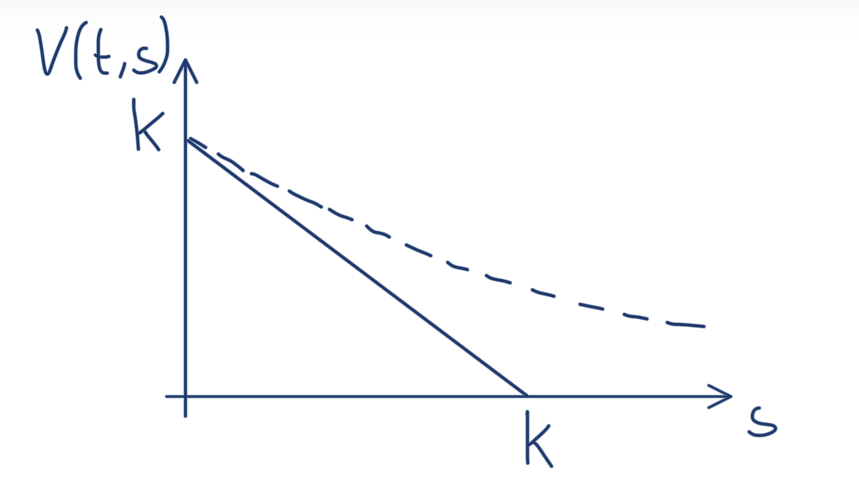
\includegraphics[width=0.7\textwidth]{images/case_1 put american.jpg}
\caption{Case 1: No early exercise anywhere}
\end{figure}

\textbf{Case 2 --- Early exercise occurs below a critical boundary}

For American puts, the situation is:

There exists a critical level $b(t)$ such that

early exercise is optimal when $s \leq b(t)$.

For $s > b(t)$, continuation is optimal:
\[
V(t, s) > [K - s]^+.
\]

Thus:

\begin{itemize}
\item $b(t)$ is the early exercise boundary.

\item It is not known explicitly, even in Black--Scholes.

\item The function $t \mapsto b(t)$ is part of the solution itself.
\end{itemize}

\begin{figure}[h]
\centering
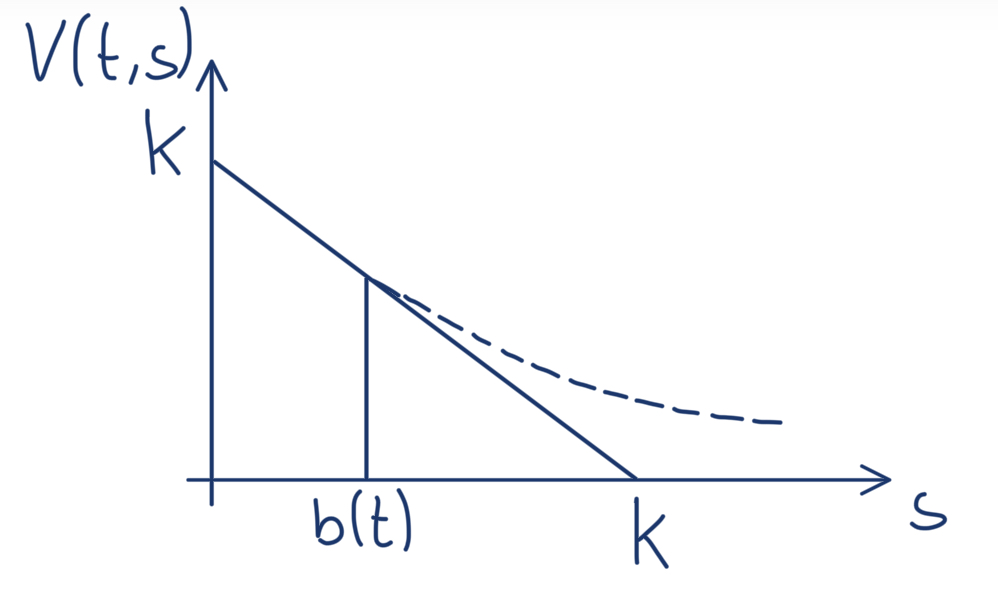
\includegraphics[width=0.7\textwidth]{images/case_2 put american.jpg}
\caption{Case 2: Early exercise occurs below a critical boundary}
\end{figure}

\paragraph{Continuation, Boundary, Stopping Regions}

The continuation region:
\[
C = \{(t, s) : V(t, s) > [K - s]^+\} = \{(t, s) : s > b(t)\}.
\]

The free boundary (the ``edge'' between continuation and stopping):
\[
\lambda C = \{(t, s) : s = b(t)\}.
\]

Early exercise is optimal in the stopping region:
\[
C^c = \{(t, s) : s \leq b(t)\}.
\]

This is a free boundary problem:

the function $b(t)$ must be solved together with the PDE.

\paragraph{Monotonicity of the Free Boundary}

It can be shown that:
\[
t < t' \implies b(t) < b(t').
\]

Thus $b(\cdot)$ is increasing in time:

as the option approaches maturity, the threshold moves upward.

\begin{figure}[h]
\centering
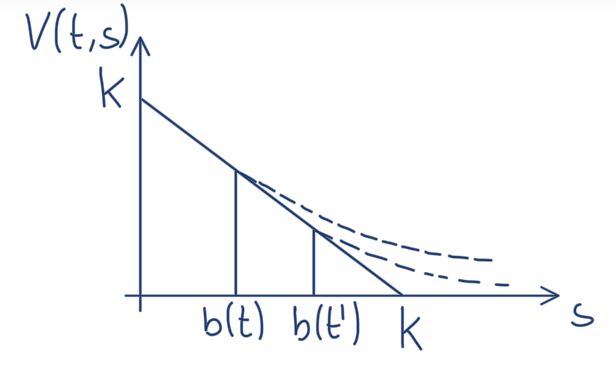
\includegraphics[width=0.7\textwidth]{images/b t and t prime.jpeg}
\caption{Monotonicity of the free boundary $b(t)$}
\end{figure}

Graphically, one clearly sees the two regions:

\begin{itemize}
\item Above $b(t)$: continuation
\item Below $b(t)$: early exercise
\end{itemize}

\begin{figure}[h]
\centering
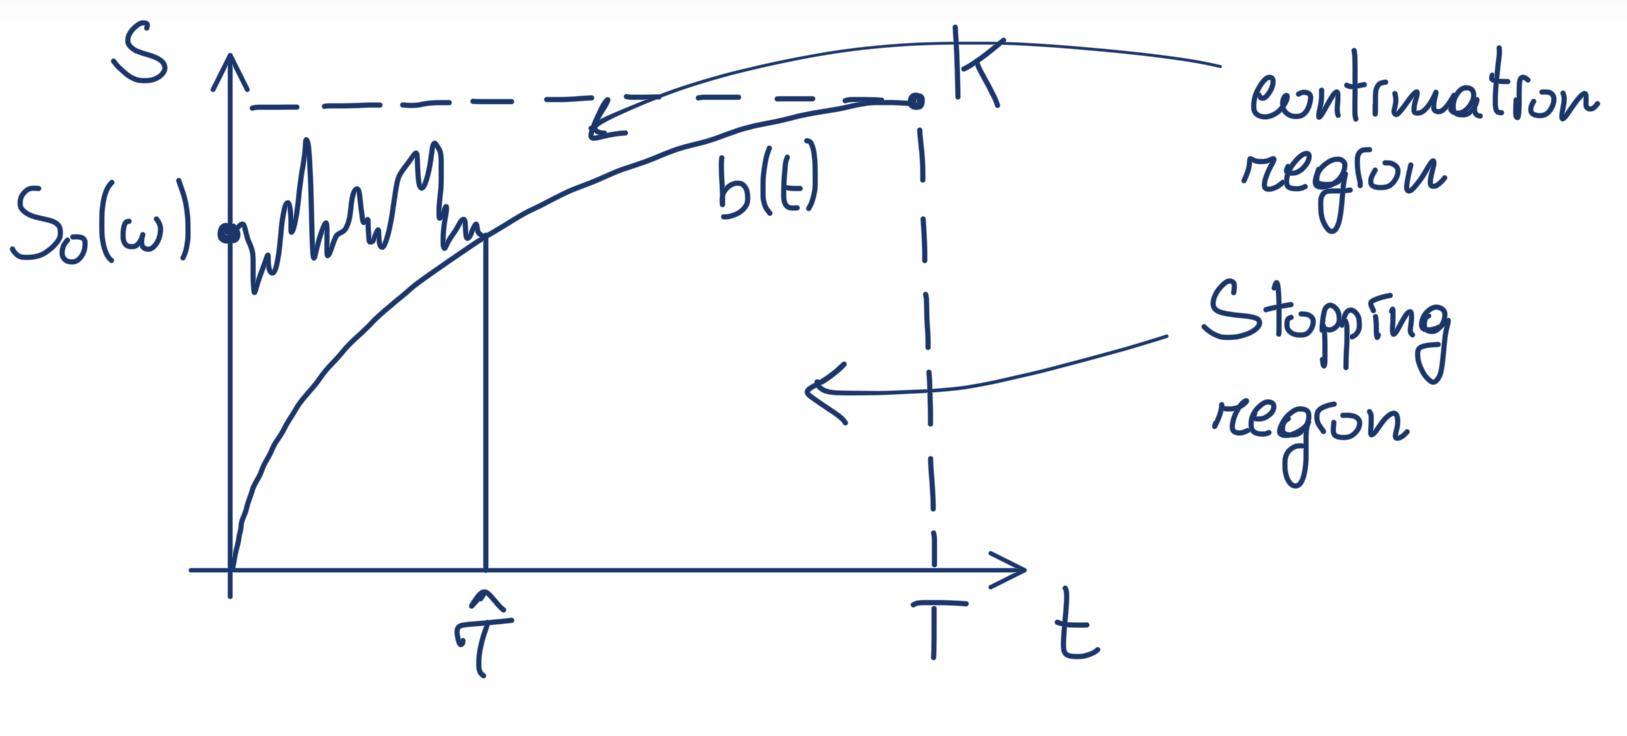
\includegraphics[width=0.7\textwidth]{images/bt chart.jpeg}
\caption{Continuation and stopping regions separated by the free boundary $b(t)$}
\end{figure}

\paragraph{Verification Theorem for the American Put}

Assume:

\begin{itemize}
\item $V \in C^{1,2}$,

\item the free boundary $\lambda C = \{(t, s) : s = b(t)\}$ with $b \in C^1$,

\item the smooth pasting condition
\[
V_s(t, b(t)) = -1 \quad \forall t \in [0, T].
\]
\end{itemize}

(This ensures regularity and guarantees that continuation/stopping meet smoothly.)

If $V$ solves:
\[
\begin{cases}
V(T, s) = [K - s]^+ & \forall s, \\
V(t, s) \geq [K - s]^+ & \forall (t, s), \\
V_t + rsV_s + \frac{1}{2}\sigma^2 s^2 V_{ss} - rV \leq 0 & \forall (t, s), \\
V(t, s) = [K - s]^+ & \forall (t, s) \in C^c, \\
V_t + rsV_s + \frac{1}{2}\sigma^2 s^2 V_{ss} - rV = 0 & \forall (t, s) \in C,
\end{cases}
\]

then:

\begin{itemize}
\item $V$ is the optimal value function of the stopping problem,

\item and the optimal stopping rule is:
\[
\hat{\tau}_{t,s} = \inf\{u \geq t : S_u = b(u)\} = \inf\{u \geq t : (u, S_u) \in \lambda C\}.
\]
\end{itemize}

This is the classical continuous-time characterization of the American put.

\subsection{Interest Rates}

\paragraph{1. Zero-Coupon Bonds (ZCBs)}

\textbf{Definition.}

A zero-coupon bond (ZCB) with maturity $T$ --- also called a $T$-bond --- is a contract that guarantees the payment of its principal at time $T$.

From now on, the principal is normalized to 1.

Price at time $t$:
\[
p(t, T).
\]

Thus, buying a ZCB at time $t$ gives you exactly 1 at time $T$.

\paragraph{2. Coupon Bonds (CBs)}

\textbf{Definition.}

A coupon bond with maturity $T$ is a contract delivering a deterministic cash-flow structure up to time $T$.

\paragraph{3. Standing Assumptions}

\textbf{Perfect market for ZCBs.}

There exists a complete market for zero-coupon bonds of all maturities $T$.

(This implies infinitely many available bonds.)

\textbf{Normalization:}
\[
p(t, t) = 1.
\]

This ensures no-arbitrage.

\textbf{Regularity of the term structure:}

For every fixed time $t$, the map
\[
T \mapsto p(t, T)
\]
is $C^1$ on $[t, T]$.

This is the usual term-structure curve observed at time $t$.

For fixed $T$, the map
\[
t \mapsto p(t, T)
\]
is a stochastic process.

Hence, the collection $\{p(t, T)\}_{T \geq t}$ is an infinite-dimensional system of SDEs---one SDE for each maturity.

\paragraph{4. Notions of Interest Rate}

Suppose that at time $t$ we enter a contract involving:

\begin{itemize}
\item an investment of 1 euro at some time $s \geq t$;
\item a repayment at time $T \geq s$.
\end{itemize}

If $t = s$, the contract is called spot;

if $t < s$, it becomes a forward interest-rate agreement.

\textbf{Constructing a forward-rate contract}

At time $t$:

\begin{itemize}
\item Sell an $s$-bond and receive $p(t, s)$.

\item Use this amount to buy
\[
\frac{p(t, s)}{p(t, T)}
\]
units of the $T$-bond.
\end{itemize}

At time $s$:

\begin{itemize}
\item You must deliver 1 euro to the buyer of the contract.
\end{itemize}

At time $T$:

\begin{itemize}
\item Your $T$-bonds mature and pay
\[
\frac{p(t, s)}{p(t, T)}.
\]
\end{itemize}

Thus this contract earns an interest over the period $[s, T]$, determined by the price ratio $p(t, s)/p(t, T)$.

\paragraph{5. Simple Forward (LIBOR) Rates}

The interest earned is determined in two equivalent ways:

\textbf{(A) Capitalization:}
\[
1 + L(t; s, T)(T - s) = \frac{p(t, s)}{p(t, T)}.
\]

\textbf{(B) Discounting:}
\[
1 = \frac{p(t, s)}{p(t, T)} - L(t; s, T)(T - s).
\]

\textbf{Definition (Forward LIBOR rate).}

The forward LIBOR rate contracted at $t$ for the period $[s, T]$ is:
\[
L(t; s, T) = -\frac{p(t, T) - p(t, s)}{(T - s)p(t, T)}.
\]

\textbf{Spot LIBOR rate.}

At $s$, the spot rate for the period $[s, T]$ is:
\[
L(s; s, T) = -\frac{p(s, T) - 1}{(T - s)p(s, T)}.
\]

\paragraph{6. Continuously Compounded Rates}

A continuously compounded interest rate $R(t; s, T)$ satisfies:
\[
1 \cdot e^{R(t; s, T)(T - s)} = \frac{p(t, s)}{p(t, T)}.
\]

\textbf{Definition (Continuously compounded forward rate).}
\[
R(t; s, T) = -\frac{1}{T - s} \ln\!\left(\frac{p(t, T)}{p(t, s)}\right).
\]

\textbf{Spot continuously compounded rate.}
\[
R(s; s, T) = -\frac{1}{T - s} \ln(p(s, T)).
\]

\paragraph{7. Instantaneous Forward Rate and Short Rate}

The instantaneous forward rate is obtained by taking the limit $s \to T$:
\[
f(t, T) = \lim_{s \to T} R(t; s, T) = -\frac{\partial}{\partial T} \ln p(t, T).
\]

\textbf{Interpretation:}

It is ``like'' the rate contracted at time $t$ over the infinitesimal interval $[T, T + dT]$.

The short rate (instantaneous spot rate) is:
\[
r(t) = f(t, t).
\]

\paragraph{8. Money Market Account}

The money market account $B_t$ grows at the instantaneous short rate:
\[
B_t = \exp\left(\int_0^t r(s) \, ds\right),
\]
that is
\[
\begin{cases}
dB_t = r(t)B_t \, dt, \\
B_0 = 1.
\end{cases}
\]

Investing in $B_t$ is equivalent to a self-financing strategy that continuously rolls over liabilities in ``just-maturing'' bonds.

\paragraph{9. Fundamental Identities}

\textbf{Lemma.}

From the definition of $f(t, T)$:
\[
p(t, T) = p(t, s) \exp\left(-\int_s^T f(t, u) \, du\right).
\]
\[
p(t, T) = \exp\!\left(-\int_t^T f(t, u) \, du\right).
\]

These are the foundational relationships between prices and instantaneous forward curves.

\paragraph{10. Models for Interest Rates}

We model interest rates in three equivalent ways.

\textbf{(A) Short-rate models}

A stochastic process $r_t$ follows:
\[
dr_t = a_t \, dt + b_t \, dW_t,
\]
where $a_t$ and $b_t$ are adapted processes, and $W_t$ is a standard Brownian motion.

\textbf{(B) Forward-rate models (Heath--Jarrow--Morton type)}

For each maturity $T$, the forward rate satisfies:
\[
df(t, T) = \alpha(t, T) \, dt + \sigma(t, T) \, dW_t.
\]

$\alpha$ and $\sigma$ may be scalar or vector-valued.

Consequently $W_t$ may be 1- or $d$-dimensional.

There is one SDE for each maturity $T$: this gives an infinite-dimensional system.

\textbf{(C) Bond price models}

The price of a bond $p(t, T)$ evolves as:
\[
dp(t, T) = p(t, T)(m(t, T) \, dt + v(t, T) \, dW_t),
\]
where:

\begin{itemize}
\item $m(t, T)$ is the drift,
\item $v(t, T)$ is the volatility (scalar or vector),
\item $W_t$ may again be multi-dimensional.
\end{itemize}

All three approaches (short rate, forward rate, bond price) are mathematically equivalent under suitable conditions.

\newpage
\section{December 1, 2025}

\subsection{Models for Bond Markets}

\paragraph{Proposition (General Relationships between Bond Prices, Forward Rates, and Short Rates)}

Under suitable assumptions, the following equivalences hold.

\textbf{1) (BP) $\Rightarrow$ (FR)}

If you specify a model for bond prices, then you are implicitly specifying the forward rate dynamics.

Bond price dynamics:
\[
dp(t, T) = p(t, T)\{m(t, T) \, dt + v(t, T) \, dW_t\} \tag{BP}
\]

Forward rate dynamics:
\[
df(t, T) = \alpha(t, T) \, dt + \sigma(t, T) \, dW_t
\]

This result also holds when $v$, $\alpha$, $W$ are vector-valued.

The link between the coefficients is:
\[
\alpha(t, T) = v_T(t, T)v(t, T) - m_T(t, T), \quad \overline{\sigma}(t, T) = \overline{v}_T(t, T).
\]

\textbf{Intuition.}

Bond prices contain information about the entire term structure. Differentiating their drift and volatility with respect to maturity $T$ gives the dynamics of the forward rates.

\textbf{2) (FR) $\Rightarrow$ (SR)}

If you specify the forward rate dynamics, then you are also specifying the short rate dynamics.

The short rate satisfies:
\[
dr_t = a_t \, dt + b_t \, dW_t,
\]
with
\[
a_t = f_T(t, t) + \alpha(t, t), \quad b_t = \sigma(t, t).
\]

\textbf{Interpretation.}

The short rate is simply the forward rate evaluated at maturity equal to the present time. Its drift and volatility are inherited directly from the forward curve dynamics.

\textbf{3) (FR) $\Rightarrow$ (BP)}

Whenever the forward rate dynamics are specified, the bond price dynamics are also fully determined.

The coefficients of the bond price SDE are:
\[
m(t, T) = r_t + A(t, T) + \frac{1}{2}\|S(t, T)\|^2,
\]
\[
v(t, T) = S(t, T),
\]
where
\[
A(t, T) = -\int_t^T \alpha(t, s) \, ds, \quad S(t, T) = -\int_t^T \sigma(t, s) \, ds.
\]

\textbf{Remark.}

This shows that specifying forward rates is mathematically equivalent to specifying the entire bond market.

\paragraph{Coupon Bond Valuation}

\textbf{Fixed Coupon Bond}

% Timeline picture from T_0 to T_n with coupons c_1, c_2, \ldots at times T_1, T_2, \ldots

The behavior of a fixed coupon bond is exactly equivalent to holding a portfolio of zero-coupon bonds (ZCBs) with different maturities. Therefore, the value of a coupon bond equals the value of the corresponding portfolio of ZCBs.

The NPV of the portfolio, hence the price of the coupon bond, is:
\[
p(t) = c_1 p(t, T_1) + \cdots + (c_n + K) p(t, T_n),
\]
where $p(\cdot, \cdot)$ denotes the price of a ZCB and $K$ is the principal.

Equivalently,
\[
p(t) = K p(t, T_n) + \sum_{i=1}^n c_i \, p(t, T_i).
\]

\textbf{Remark (Standard Market Conventions)}

Typically,
\[
c_i = r_i \, (T_i - T_{i-1}) \, K,
\]
where $r_i$ is the interest rate prevailing on the interval $[T_{i-1}, T_i)$.

At inception, all rates are known and usually constant.

Often,
\[
r_i \equiv r, \quad T_i - T_{i-1} \equiv \delta,
\]
so that
\[
c = r \, \delta \, K,
\]
and therefore
\[
p(t) = K p(t, T_n) + r \, \delta \, K \sum_{i=1}^n p(t, T_i).
\]

\textbf{Floating Rate Coupon Bond}

Usually, the floating rate is linked to a financial benchmark (e.g. LIBOR) or to a non-financial index (e.g. inflation).

Assume:
\[
r_i = L(T_{i-1}, T_i),
\]
then
\[
c_i = (T_i - T_{i-1}) \, L(T_{i-1}, T_i) \, K.
\]

\paragraph{Evaluation of a Floating Rate Coupon Bond at $t < T_0$}

Assume:
\[
K = 1, \quad T_i - T_{i-1} \equiv \delta \quad \forall i.
\]

Then:
\[
c_i = \delta \, L(T_{i-1}, T_i) = \delta \frac{1 - p(T_{i-1}, T_i)}{\delta \, p(T_{i-1}, T_i)} = \frac{1}{p(T_{i-1}, T_i)} - 1.
\]

\textbf{Interpretation as a Self-Financing Strategy}

The payoff $\frac{1}{p(T_{i-1}, T_i)}$ can be replicated as follows:

\begin{itemize}
\item At time $t$, buy one bond with price $p(t, T_{i-1})$.

\item At time $T_{i-1}$, the bond matures and delivers 1€.

\item Use it to buy $\frac{1}{p(T_{i-1}, T_i)}$ bonds maturing at $T_i$.

\item At time $T_i$, these bonds mature and pay:
\[
\frac{1}{p(T_{i-1}, T_i)}.
\]
\end{itemize}

Thus:
\[
\Pi_t\!\left(\frac{1}{p(T_{i-1}, T_i)}\right) = p(t, T_{i-1}).
\]

Moreover, the value at time $t$ of 1€ paid at time $T_i$ is:
\[
\Pi_t(1) = p(t, T_i).
\]

Hence, the value at time $t$ of the coupon $c_i$ paid at $T_i$ is:
\[
\Pi_t\!\left(\frac{1}{p(T_{i-1}, T_i)}\right) - \Pi_t(1) = p(t, T_{i-1}) - p(t, T_i).
\]

\paragraph{Value at Time $t$ of the Floating Rate Coupon Bond}

\begin{align*}
p(t) &= \Pi_t(1) + \sum_{i=1}^n \Pi_t(c_i) \\
&= p(t, T_n) + \sum_{i=1}^n [p(t, T_{i-1}) - p(t, T_i)] \\
&= p(t, T_n) + p(t, T_0) - p(t, T_n) \\
&= p(t, T_0), \quad \text{for } t < T_0.
\end{align*}

\textbf{Key result.}

The value of a floating rate coupon bond is exactly equal to the price of the zero-coupon bond maturing at the next reset date $T_0$.

\subsection{Valuation of Interest Rate Swaps (IRS)}

A swap is a derivative contract in which two counterparties exchange a fixed interest rate for a floating interest rate.

\paragraph{Contract Characteristics}

\begin{itemize}
\item \textbf{Principal (or Notional) value:} $K$

\item $T_0$ is the emission date

\item $T_1, \ldots, T_n$ are the payment dates

\item The time spacing is constant:
\[
T_i - T_{i-1} \equiv \delta, \quad \forall i
\]

\item \textbf{Fixed leg:} stream of payments at fixed rate $R$ (swap rate)

\item \textbf{Floating leg:} stream of payments at floating rate:
\[
L(T_{i-1}, T_i), \quad \forall i
\]
(typically LIBOR)
\end{itemize}

A payer swap is a contract in which the holder pays the fixed rate and receives the floating rate.

% Picture of the payer swap

\paragraph{Fair Value Principle of a Swap}

At inception, the value of the swap must be:
\[
p(t) = 0
\]
since no money is exchanged at initiation. Hence, the net present value (NPV) of all future cash flows must be zero.

The swap rate $R$ is therefore chosen such that:
\[
\text{NPV} = 0 \iff p(t) = 0.
\]

\paragraph{Cash Flows of the Payer Swap}

At each payment date $T_i$, the cash flow is:
\[
\text{CF}_i = K\delta[L(T_{i-1}, T_i) - R].
\]

The value at time $t$ of this cash flow is:
\[
\Pi_t(\text{CF}_i) = K[p(t, T_{i-1}) - p(t, T_i)] - K\delta R \, p(t, T_i).
\]

\paragraph{Total Value of the Swap at Time $t$}

\begin{align*}
p(t) &= \sum_{i=1}^n \Pi_t(\text{CF}_i) \\
&= K \sum_{i=1}^n [p(t, T_{i-1}) - p(t, T_i)] - K\delta R \sum_{i=1}^n p(t, T_i) \\
&= K p(t, T_0) - \sum_{i=1}^n K d_i \, p(t, T_i),
\end{align*}

where
\[
d_i = \begin{cases}
\delta R, & i = 1, \ldots, n-1, \\
1 + \delta R, & i = n.
\end{cases}
\]

Starting from this valuation formula, we impose:
\[
p(t) = 0,
\]
which allows us to compute the par swap rate $R$.

\paragraph{Par Swap Rate (General Case)}

For $t = 0$, we obtain:
\[
R = \frac{p(0, T_0) - p(0, T_n)}{\delta \sum_{i=1}^n p(0, T_i)}.
\]

This determines the fair fixed rate such that the swap has zero NPV at inception.

\paragraph{Special Case: $t = T_0 = 0$}

Since $p(0, T_0) = 1$, we obtain:
\[
R = \frac{1 - p(0, T_n)}{\delta \sum_{i=1}^n p(0, T_i)}.
\]

This is the standard market formula for the par swap rate.

\paragraph{Financial Interpretation}

\begin{itemize}
\item The floating leg replicates a sequence of forward loans.

\item The fixed leg is equivalent to a coupon bond with fixed coupon $K\delta R$.

\item The par rate equates the market value of these two legs.

\item Conceptually, the swap is a zero-cost exchange of two bond portfolios.
\end{itemize}

\subsection{Yield Curve and Duration}

We can evaluate the IRR (Internal Rate of Return) of any stream of cash flows.

\paragraph{Zero Coupon Bond (ZCB)}

Consider a bond that pays 1€ at time $T$.

At time $t$, its price is $p(t, T)$.

The associated cash flows are:
\[
\{(t, -p(t, T)), \ (T, 1)\}.
\]

The IRR of this investment is the yield $y = y(t, T)$, called the yield to maturity, defined as the solution of:
\[
e^{-y(T - t)} = p(t, T).
\]

Therefore, the ZCB yield is:
\[
y(t, T) = -\frac{\ln p(t, T)}{T - t} = R(t, T).
\]

The function:
\[
T \longmapsto y(t, T)
\]
is called the yield curve.

\textbf{Interpretation.}

The yield curve describes the term structure of interest rates expressed in terms of yields rather than prices.

\paragraph{Coupon Bonds (CB)}

For a coupon bond we have the cash-flow stream:
\[
\{(t, -p(t)); (T_1, c_1); \ldots; (T_n, c_n)\}.
\]

The Yield to Maturity (YTM) of this coupon bond is the rate $y = y(t)$ such that:
\[
p(t) = \sum_{i=1}^n c_i e^{-y(T_i - t)}.
\]

This equation generally cannot be solved in closed form and must be solved numerically.

\paragraph{Macaulay Duration}

\textbf{Definition}

The Macaulay Duration of the coupon bond at $t = 0$ is:
\[
D = \frac{\sum_{i=1}^n T_i c_i e^{-y T_i}}{p(0)} = \frac{\sum_{i=1}^n T_i c_i e^{-y T_i}}{\sum_{i=1}^n c_i e^{-y T_i}}.
\]

We can interpret it as the weighted average of the payment dates, where the weights are given by the present value of each coupon.

Thus, $D$ represents:

\begin{itemize}
\item the mean duration,
\item the mean time to coupon payment.
\end{itemize}

\textbf{Intuitive Explanation of Duration}

Duration measures the effective maturity of a bond:

it tells us when, on average, the investor gets their money back, in present-value terms.

\begin{itemize}
\item A ZCB has duration exactly equal to its maturity.

\item A coupon bond has duration strictly smaller than its final maturity, because part of the cash flows are received earlier.

\item The higher the coupons, the shorter the duration.

\item The lower the yield, the larger the duration.
\end{itemize}

From a risk-management point of view, duration measures the bond's sensitivity to interest-rate variations, exactly as delta measures price sensitivity in option pricing.

\paragraph{Sensitivity of the Bond Price to Yield}

\textbf{Proposition}
\[
\frac{\partial p}{\partial y} = -D \, p.
\]

Hence, $D$ plays for bonds the same role as delta for options.

This relation gives the first-order approximation:
\[
\frac{\Delta p}{p} \approx -D \, \Delta y.
\]

\paragraph{Convexity}

Convexity plays the same role as Gamma in options.

It is defined as:
\[
C = \frac{\partial^2 p}{\partial y^2}.
\]

Convexity measures the second-order sensitivity of the bond price with respect to changes in the yield and corrects the linear (duration-based) approximation for large yield movements.

\subsection{Short Rate (SR) Models}

The short rate follows the stochastic differential equation:
\[
dr_t = b(t, r_t) \, dt + \sigma(t, r_t) \, dW_t, \tag{SR}
\]
where $b$, $\sigma$ are real-valued functions and the short rate $r_t$ is not a traded asset.

The bank account (money market account) evolves as:
\[
\begin{cases}
dB_t = r_t B_t \, dt, \\
B_0 = 1.
\end{cases}
\]

\paragraph{Market Incompleteness}

The market is incomplete.

\textbf{Meta-theorem.}

Let $M$ be the number of risky traded assets and $R$ the number of risk factors.

If $M < R$, then the market is incomplete.

Here:
\[
M = 0 \text{ (no risky traded assets)}, \quad R = 1 \text{ (one Brownian motion)},
\]
hence $M < R \Rightarrow$ market incompleteness.

\paragraph{Bond Market Generated by the Short Rate}

Consider a market of zero-coupon bonds (T-bonds) for all $T > 0$, viewed as derivatives written on the short rate.

\textbf{Assumption}

For all $T > 0$, the price at time $t$ of a T-bond is:
\[
p(t, T) = F(t, r_t; T) = F_T(t, r_t),
\]
with
\[
F_T \in C^{1,2}.
\]

This assumption implies that there exist functional relations among all functions $F_T$.

\paragraph{Step-by-Step Construction}

\textbf{1) Selection of Two Bonds}

Consider two bonds with maturities:
\[
T > 0, \quad S > 0.
\]

\textbf{2) Market with Assets $(B, F_T, F_S)$}

Apply Itô's formula to $F_T(t, r_t)$:
\[
dF_T(t, r_t) = \alpha_T F_T \, dt + \sigma_T F_T \, dW_t,
\]
where:
\[
\alpha_T = \frac{1}{F_T}\left(F_t^T + bF_r^T + \frac{\sigma^2}{2}F_{rr}^T\right), \quad \sigma_T = \frac{\sigma F_r^T}{F_T}.
\]

An analogous expression holds for $F_S$.

\textbf{3) Self-Financing Portfolio}

Construct a self-financing portfolio:
\[
\overline{h} = (u_T, u_S).
\]

Its value process $V_t^h$ satisfies:
\[
dV_t^h = V_t^h([u_S \alpha_S + u_T \alpha_T] \, dt + [u_S \sigma_S + u_T \sigma_T] \, dW_t).
\]

\textbf{4) Elimination of Risk}

Choose the portfolio weights such that:
\[
\begin{cases}
u_S + u_T = 1, \\
u_S \sigma_S + u_T \sigma_T = 0.
\end{cases}
\]

We have:
\[
u_S = \frac{\sigma_T}{\sigma_T - \sigma_S}, \quad u_T = - \frac{\sigma_S}{\sigma_T - \sigma_S}.
\]

Substituting those terms, we end up with the final formula:
\[
dV_t^h = V_t^h\left\{\frac{\alpha_S \sigma_T - \alpha_T \sigma_S}{\sigma_T - \sigma_S}\right\} dt.
\]

This portfolio is locally riskless.

\textbf{5) No-Arbitrage Condition}

By No Arbitrage (NA), the drift of this locally riskless portfolio must equal the short rate:
\[
\frac{\alpha_S \sigma_T - \alpha_T \sigma_S}{\sigma_T - \sigma_S} = r_t.
\]

This is equivalent to:
\[
\frac{\alpha_S(t, r_t) - r_t}{\sigma_S(t, r_t)} = \frac{\alpha_T(t, r_t) - r_t}{\sigma_T(t, r_t)}, \quad \forall t \in [0, T], \quad \mathbb{P}\text{-a.s.}
\]

\paragraph{Market Price of Risk}

Since the ratio is constant with respect to maturity $T$, we obtain the result:

\textbf{Proposition}

There exists a process $\lambda = \{\lambda_t\}_{t \geq 0}$ such that:
\[
\forall T > 0, \quad \frac{\alpha_T(t, r_t) - r_t}{\sigma_T(t, r_t)} = \lambda_t.
\]

The process $\lambda_t$ is the market price of risk.

It is a market characteristic not specified by the model and must be given exogenously.

\paragraph{Term Structure Equation}

Assume:

\begin{itemize}
\item $r_t$ has full support on $\mathbb{R}$,

\item $\lambda_t = \lambda(t, r_t)$, i.e. the market price of risk is a deterministic function of $(t, r_t)$.
\end{itemize}

Then the bond price function $F_T$ solves the term structure PDE:
\[
\begin{cases}
F_t^T + (b - \lambda\sigma) \, F_r^T + \frac{\sigma^2}{2}F_{rr}^T - rF_T = 0, \\
F_T(T, r) = p(T, T) = 1.
\end{cases}
\]

This is the fundamental valuation equation for zero-coupon bonds in SR models.

\paragraph{Risk-Neutral Valuation Formula}

By Itô's formula and Girsanov's theorem, one obtains the representation:
\[
p(t, T) = F_T(t, r) = \mathbb{E}_{t,r}^{\mathbb{Q}}\!\left[e^{-\int_t^T r_s \, ds}\right].
\]

This shows that the bond price is the risk-neutral expectation of the stochastic discount factor generated by the short rate.

\newpage
\section{December 4, 2025}

\subsection{Short-Rate Models and Affine Term Structure}

\subsubsection{The Fundamental Pricing Equation}

We begin by defining the price of a Zero-Coupon Bond (ZCB) with maturity $T$ at time $t$. The fundamental pricing formula in a no-arbitrage framework is given by the expectation of the discount factor:
\[
p(t,T) = F(t,r;T) = \E^{\Q}\left[e^{-\int_t^T r_s \, ds}\right]
\]

\textbf{Theoretical Context:} Here, $\Q = \Q_\lambda$ refers to the Risk-Neutral Measure. It is specific in the sense that it depends on the market price of risk, denoted by $\lambda$. Under this measure, the discounted asset prices are martingales.

The dynamics of the short rate $r_t$ under the measure $\Q$ are governed by the following Stochastic Differential Equation (SDE):
\[
\begin{cases}
dr_s = \{b(s,r_s) - \lambda(s,r_s)\sigma(s,r_s)\}\,ds + \sigma(s,r_s)\,dW_s^{\Q} \\
r_t = r
\end{cases}
\]

To simplify notation, we define the risk-neutral drift $\mu$ as:
\[
\mu(s,r_s) = b(s,r_s) - \lambda(s,r_s)\sigma(s,r_s)
\]

This represents the drift of the short rate after adjusting for the risk premium.

\subsubsection{Pricing General $T$-Claims}

\textbf{Bridge:} The formula above applies specifically to bonds (which pay 1 at maturity). However, we can generalize this to any derivative contract.

\begin{remark}
If we have a general $T$-claim (a derivative expiring at $T$) with payoff $X = \Phi(r_T)$, its price $\Pi_t(X)$ is given by:
\[
\Pi_t(X) = \E_{t,r}^{\Q}\left[X e^{-\int_t^T r_s \, ds}\right]
\]

From the perspective of the Term Structure Equation (TSE)—which is the Partial Differential Equation (PDE) governing these prices—the payoff becomes the terminal condition:
\[
F(T,r) = \Phi(r)
\]

(For a bond, $\Phi(r) = 1$, hence $F(T,r) = 1$.)
\end{remark}

\subsubsection{Model Calibration (Inversion of the Yield Curve)}

\textbf{Intuition:} A key challenge in finance is choosing the correct measure $\Q$. Since $\Q$ depends on $\lambda$ (the market price of risk), choosing $\Q$ is equivalent to calibrating $\lambda$.

We calibrate $\lambda$ (and therefore choose $\Q_\lambda$) by observing the market prices of bonds. This process is often called the \textit{inversion of the yield curve}. The procedure follows these logical steps:

\begin{enumerate}
\item \textbf{Parametric Assumption:} Suppose you have a parametric model for the coefficients. Let $\boldsymbol{\alpha} \in \R^k$ be a vector of parameters such that:
\[
b(t,r;\boldsymbol{\alpha}), \quad \sigma(t,r;\boldsymbol{\alpha})
\]
Consequently, both the risk-neutral drift $\mu$ and the risk premium $\lambda$ depend on $\boldsymbol{\alpha}$.

\item \textbf{Theoretical Calculation:} Compute the theoretical Term Structure (TS) of bond prices based on these parameters:
\[
\{p(t,T;\boldsymbol{\alpha})\}_T
\]

\item \textbf{Data Collection:} At time $t=0$, collect the currently observed market Term Structure:
\[
\{p^*(0,T)\}_{T>0}
\]

\item \textbf{Fitting:} Fit the parameters $\boldsymbol{\alpha}^*$ to match the observed Term Structure (usually via Least Squares minimization).

\item \textbf{Measure Specification:} Once $\boldsymbol{\alpha}^*$ is found, we fix the dynamics:
\[
\mu^*(t,r) = \mu(t,r;\boldsymbol{\alpha}^*), \quad \sigma^*(t,r) = \sigma(t,r;\boldsymbol{\alpha}^*)
\]
This uniquely identifies the measure $\Q = \Q_\lambda$.

\item \textbf{Pricing:} Use this specific $\Q$ to price other Interest Rate (IR) derivatives.
\end{enumerate}

\textbf{What is the ``problem'' in this scheme?} The main issue lies at point 2). We are attempting to capture the entire term structure (which is an infinite-dimensional object) using a finite number of parameters ($\boldsymbol{\alpha} \in \R^k$). Often, the parameters are not flexible enough to fit the market curve perfectly, leading to calibration errors.

\subsubsection{Affine Term Structure (ATS)}

\textbf{Learning Note:} Solving the Term Structure PDE numerically for every calibration step is computationally expensive. We prefer models where the solution has a closed analytical form. This leads us to Affine Models.

\begin{definition}
A model admits an \textbf{Affine Term Structure (ATS)} if the bond price term structure $\{p(t,T): 0 \leq t \leq T, T > 0\}$ takes the specific exponential form:
\[
p(t,T) = e^{A(t,T) - r_t B(t,T)}
\]
where $A(t,T)$ and $B(t,T)$ are deterministic functions parameterized by $T$.
\end{definition}

\paragraph{Martingale Modeling and Dynamics}

We specify the dynamics of $r$ under $\Q$. The following proposition provides sufficient conditions for a model to be Affine.

\begin{proposition}
Assume that the drift and diffusion take the following linear and square-root forms (with deterministic coefficients $\alpha,\beta,\gamma,\delta$):
\[
\begin{cases}
\mu(t,r) = \alpha(t)r + \beta(t) \\
\sigma(t,r) = \sqrt{\gamma(t)r + \delta(t)}
\end{cases}
\]

Then, the model admits an ATS, where the functions $A$ and $B$ satisfy the following system of Ordinary Differential Equations (ODEs):

\begin{enumerate}
\item The Riccati ODE for $B$:
\[
\begin{cases}
B_t(t,T) + \alpha(t)B(t,T) - \frac{\gamma(t)}{2}B^2(t,T) + 1 = 0 \\
B(T,T) = 0
\end{cases}
\]

\item The Linear ODE for $A$:
\[
\begin{cases}
A_t(t,T) = \beta(t)B(t,T) - \frac{\delta(t)}{2}B^2(t,T) \\
A(T,T) = 0
\end{cases}
\tag{$*$}
\]
\end{enumerate}
\end{proposition}

\subsubsection{Proof of the Proposition}

\textbf{Strategy:} To prove this, we assume the affine form $F_T(t,r) = e^{A - rB}$, compute its partial derivatives, substitute them into the general Term Structure Equation (PDE), and force the equation to hold for all values of $r$.

Fix $T > 0$. We look for functions $A,B$ such that the bond price $F_T(t,r) = e^{A(t,T) - rB(t,T)}$ solves the TSE.

\paragraph{Step 1: Compute Derivatives}
\[
\begin{aligned}
F_t^T(t,r) &= F_T(t,r)[A_t(t,T) - rB_t(t,T)] \\
F_r^T(t,r) &= -F_T(t,r)B(t,T) \\
F_{rr}^T(t,r) &= F_T(t,r)B^2(t,T)
\end{aligned}
\]

\paragraph{Step 2: Substitute into the PDE} 

The general Term Structure Equation is $F_t + \mu F_r + \frac{1}{2}\sigma^2 F_{rr} - rF = 0$. Substituting our dynamics and derivatives:
\[
F_T(t,r)\left\{\underbrace{A_t - rB_t}_{\text{from } F_t} \underbrace{- B[\alpha(t)r + \beta(t)]}_{\text{from } \mu F_r} + \underbrace{\frac{1}{2}B^2[\gamma(t)r + \delta(t)]}_{\text{from } \frac{1}{2}\sigma^2 F_{rr}} - r\right\} = 0
\]

\paragraph{Step 3: Boundary Conditions} 

From the terminal condition $F_T(T,r) = 1$, we have:
\[
\exp\{A(T,T) - rB(T,T)\} = 1
\]

For this to equal 1 for any $r$, the exponent must be zero. This happens if and only if:
\[
A(T,T) = 0 \quad \text{and} \quad B(T,T) = 0
\]

\paragraph{Step 4: Separation of Variables} 

Let's analyze the expression inside the curly brackets in the PDE. Since $F_T \neq 0$, the term inside the brackets must be zero. We group terms multiplied by $r$ and terms without $r$:
\[
\underbrace{A_t(t,T) - B(t,T)\beta(t) + \frac{\delta(t)}{2}B^2(t,T)}_{\text{Terms independent of } r} - r\underbrace{[B_t(t,T) + \alpha(t)B(t,T) - \frac{\gamma(t)}{2}B^2(t,T) + 1]}_{\text{Terms linear in } r} = 0
\]

For this equation to hold for any state of the short rate $r$, both parts must independently be equal to zero. This yields precisely our system:

\begin{itemize}
\item The term multiplying $r$ gives the Riccati ODE.
\item The term independent of $r$ gives the equation ($*$) for $A$.
\end{itemize}

Thus, the proposition holds.

\subsection{Examples of Specific Models}

Having established the general theory of Affine Term Structures (ATS), we now examine two fundamental one-factor models used in the industry: the Vasicek model and the Cox-Ingersoll-Ross (CIR) model.

\subsubsection{The Vasicek Model}

The Vasicek model (1977) assumes that the short rate process evolves according to an Ornstein-Uhlenbeck process. The dynamics under the risk-neutral measure $\Q$ are given by:
\[
dr_t = a(b - r_t)\,dt + \sigma\,dW_t^{\Q}, \quad a > 0
\]

\textbf{Alternative Parameterization:} It is often more intuitive to rewrite the drift term to highlight the mean-reverting behavior. We define $k = a$ and $\vartheta = b/a$. The SDE then becomes:
\[
dr_t = k(\vartheta - r_t)\,dt + \sigma\,dW_t^{\Q}
\]

These are two equivalent representations of the same dynamics.

\paragraph{Properties of the Vasicek Model}

\begin{enumerate}
\item \textbf{Gaussian Distribution:} The SDE is linear in $r_t$, and the volatility coefficient $\sigma$ is constant. Consequently, the short rate $r_t$ (and the resulting bond prices) follows a Gaussian (Normal) distribution. This allows for explicit analytical solutions for bond prices and option prices.

\item \textbf{Possibility of Negative Rates:} A major characteristic (often considered a drawback in classical theory) is that the Gaussian distribution supports the entire real line. At any time $t$, there is a non-zero probability that the interest rate becomes negative:
\[
\Q(r_t < 0) > 0
\]

\item \textbf{Asymptotic Mean:} The expectation of the short rate converges to the long-term level $\vartheta$ as time goes to infinity:
\[
\lim_{t \to +\infty} \E[r_t] = \vartheta = \frac{b}{a}
\]

\item \textbf{Mean Reversion:} The parameter $k$ represents the speed of mean reversion, while $\vartheta$ represents the long-term mean level. We can analyze the drift to understand this ``pulling'' mechanism:

\begin{itemize}
\item If $r_t = \vartheta$: The drift is zero. On average, the rate remains stable over the interval $[t,t+dt)$.

\item If $r_t > \vartheta$: The drift $k(\vartheta - r_t)$ is negative. On average, $r_s$ will decrease over $[t,t+dt)$, being pulled back down toward the mean.

\item If $r_t < \vartheta$: The drift is positive. On average, $r_s$ will increase over $[t,t+dt)$, being pushed back up toward the mean.
\end{itemize}

Indeed, for this reason, $r_t$ is called a \textit{mean-reverting process}.

\item \textbf{Calibration Limitation:} As discussed in the previous section regarding the ``inversion of the yield curve,'' this model relies on only three parameters $(a,b,\sigma)$ or $(k,\vartheta,\sigma)$. These are generally not enough to perfectly match the observed market term structure $p^*(0,T)$ for all maturities $T > 0$.
\end{enumerate}

\subsubsection{The CIR (Cox-Ingersoll-Ross) Model}

The CIR model (1985) improves upon Vasicek by introducing a state-dependent volatility term to preclude negative interest rates. The dynamics are:
\[
dr_t = k(\vartheta - r_t)\,dt + \sigma\sqrt{r_t}\,dW_t^{\Q}
\]

\paragraph{Key Properties:}

\begin{enumerate}
\item \textbf{Non-Gaussian:} Due to the square-root diffusion term ($\sqrt{r_t}$), the process is non-Gaussian. (It actually follows a non-central chi-squared distribution).

\item \textbf{Positivity and the Feller Condition:} The square root term $\sqrt{r_t}$ naturally requires $r_t \geq 0$. However, to ensure the rate stays strictly positive and never touches zero (which could cause technical issues), the parameters must satisfy the \textbf{Feller Condition}:
\[
2k\vartheta > \sigma^2 \quad \Longrightarrow \quad r_t > 0 \quad \Q\text{-a.s.}
\]

If this condition holds, the drift is strong enough at low levels to push the rate away from zero before the volatility can drive it to hit the boundary.

\item \textbf{Intuition:} This makes the CIR model a suitable choice if you require positive interest rates, or if you are modeling a general economic factor that must remain positive (such as a default intensity or hazard rate in credit risk).
\end{enumerate}

\subsubsection{Hull-White Model (Extended Vasicek)}

The Hull-White model extends the Vasicek framework by allowing the parameters to be time-dependent. This flexibility is essential for fitting the model to market data. The dynamics of the short rate are given by:
\[
dr_t = [\vartheta(t) - a(t)r_t]\,dt + \sigma(t)\,dW_t^{\Q}
\]

Here, $\vartheta(t)$, $a(t)$, and $\sigma(t)$ are deterministic functions, and we assume $a(t) > 0$.

\paragraph{Key Properties:}

\begin{enumerate}
\item \textbf{Gaussian:} Like Vasicek, $r_t$ follows a Gaussian distribution. Consequently, it retains the drawback that interest rates can become negative.

\item \textbf{Perfect Calibration:} In the Vasicek model, we had constant scalars $(a,b,\sigma)$. Here, because we are specifying functions of time, we effectively have an infinite number of parameters (a possible value for every $t$). This flexibility allows the model to fit the observed initial yield curve $p^*(0,T)$ perfectly.
\end{enumerate}

\subsection{Forward Rate Models: The HJM Framework}

\textbf{Bridge:} While short-rate models (like Vasicek/Hull-White) start with $r_t$ and derive bond prices, the Heath-Jarrow-Morton (HJM) framework takes a different approach. It models the entire forward rate curve directly.

To achieve a perfect fit to market data, we model the dynamics of the instantaneous forward rate $f(t,T)$ for all maturities $T$. This means we are modeling an infinite number of processes simultaneously (one for each maturity date $T$).

\subsubsection{Dynamics:}

\[
\begin{cases}
df(t,T) = \alpha(t,T)\,dt + \boldsymbol{\sigma}(t,T)\,d\boldsymbol{W}_t^{\Q} \\
f(0,T) = f^*(0,T) \quad \text{(observed forward rate structure)}
\end{cases}
\]

\paragraph{Structural Links:}

The short rate is simply the forward rate for immediate maturity:
\[
r_t = f(t,t), \quad t \geq 0
\]

Using the fundamental pricing formula for a bond, $p(t,T) = \exp\{-\int_t^T f(t,u)\,du\}$, and the relationship $\Pi_0(X) = \E^{\Q}[Xe^{-\int_0^T r_s \, ds}]$, specifying the forward rate dynamics automatically determines the whole term structure.

\paragraph{The Problem of Arbitrage:} 

In this setup, we have a $d$-dimensional Brownian Motion ($\boldsymbol{W}_t \in \R^d$), so the rank of the noise is $R = d$. However, we are modeling a curve with infinite points ($M = +\infty$). According to the Meta-Theorem of Arbitrage, if we choose $\alpha$ and $\sigma$ arbitrarily, the market allows for arbitrage. To ensure No Arbitrage (NA), we must impose an internal consistency relationship between the drift $\alpha$ and the volatility $\sigma$.

\subsubsection{Theorem: The HJM Drift Condition}

Assume the Forward Rate dynamics are given under the risk-neutral measure $\Q$. To ensure the absence of arbitrage (NA), the drift term $\alpha(t,T)$ must satisfy:
\[
\alpha(t,T) = \sigma(t,T) \int_t^T \sigma(t,s)\,ds
\]

(Note: If $\sigma$ is a vector, this is the dot product).

\paragraph{Proof}

\textbf{Strategy:} We derive the dynamics of the bond price $p(t,T)$ starting from the dynamics of the forward rates $f(t,T)$. We then apply the standard no-arbitrage condition: under $\Q$, the local mean rate of return of any traded asset must equal the short rate $r_t$.

\textit{Step 1: From Forward Rates to Bond Prices}

By Ito's Lemma (specifically the version for integrals of stochastic processes), the dynamics of the bond price $p(t,T)$ are:
\[
dp(t,T) = p(t,T)\left\{[r_t + A(t,T) + \frac{1}{2}S^2(t,T)]\,dt + S(t,T)\,dW_t^{\Q}\right\}
\]

Where we define the auxiliary terms $A$ and $S$ as integrals of the forward parameters:
\[
A(t,T) = -\int_t^T \alpha(t,s)\,ds \quad \text{and} \quad S(t,T) = -\int_t^T \sigma(t,s)\,ds
\]

\textit{Step 2: Enforcing No Arbitrage}

If No Arbitrage holds, the drift of the bond price (the term in square brackets) must equal $r_t p(t,T)$.
\[
\text{Drift} = r_t \quad \Longrightarrow \quad r_t + A(t,T) + \frac{1}{2}S^2(t,T) = r_t
\]

Canceling $r_t$, we get the condition:
\[
A(t,T) + \frac{1}{2}S^2(t,T) = 0
\]

\textit{Step 3: Differentiation}

To isolate the relationship between $\alpha$ and $\sigma$, we differentiate this equation with respect to $T$:
\[
\frac{\partial}{\partial T}A(t,T) + \frac{\partial}{\partial T}\left(\frac{1}{2}S^2(t,T)\right) = 0
\]

Recall that $\frac{\partial}{\partial T}\int_t^T g(s)\,ds = g(T)$. Therefore:
\[
\frac{\partial A}{\partial T} = -\alpha(t,T)
\]
\[
\frac{\partial}{\partial T}\left(\frac{1}{2}S^2\right) = S(t,T) \cdot \frac{\partial S}{\partial T} = S(t,T)[-\sigma(t,T)]
\]

Substituting these back:
\[
-\alpha(t,T) + S(t,T)[-\sigma(t,T)] = 0
\]
\[
\Longrightarrow \quad \alpha(t,T) = -S(t,T)\sigma(t,T)
\]

Substituting the definition of $S(t,T)$ back in, we obtain the HJM drift condition:
\[
\alpha(t,T) = \sigma(t,T)\int_t^T \sigma(t,s)\,ds
\]

\begin{remark}
If $d > 1$, $S^2(t,T)$ becomes $\int_t^T \|\sigma(t,s)\|^2\,ds$ in the notation, but the vector logic remains the same: $\alpha = \sigma \cdot (\int \sigma)$.
\end{remark}

\subsubsection{HJM Implementation Algorithm}

Because $\alpha$ is determined by $\sigma$, the calibration process is simplified:

\begin{enumerate}
\item \textbf{Choose $\sigma(t,T)$:} This is the only free parameter.

\item \textbf{Impose Consistency:} Calculate $\alpha(t,T)$ using the Drift Condition.

\item \textbf{Collect Data:} Observe the initial forward curve $f^*(0,T)$ from the market.

\item \textbf{Simulate:} The forward rate at time $t$ is:
\[
f(t,T) = f^*(0,T) + \int_0^t \alpha(s,T)\,ds + \int_0^t \sigma(s,T)\,dW_s^{\Q}
\]

\item \textbf{Compute $r_t$:} Set $r_t = f(t,t)$ and use this to price IR derivatives.
\end{enumerate}

\subsection{Change of Numeraire}

\textbf{Theoretical Context:} In many complex pricing scenarios (like pricing options on bonds), the standard risk-neutral measure $\Q$ (where the bank account is the numeraire) makes integrals hard to solve. Changing the numeraire can simplify the expectation term.

Consider a market with $n+1$ traded assets $S^0, \ldots, S^n$ with continuous trajectories.

\begin{definition}
If an asset $S_t^i > 0$ almost surely for all $t \geq 0$, then $S^i$ can serve as a \textbf{numeraire}.
\end{definition}

\subsubsection{1st Fundamental Theorem of Asset Pricing (1FTAP):}

There is ``No Free Lunch with Vanishing Risk'' (NFLVR) if and only if there exists a measure $\Q^0$, called an \textbf{Equivalent Local Martingale Measure (ELMM)}, associated with the numeraire $S^0$, such that:

\begin{enumerate}
\item $\Q^0 \sim \Prob$ (Equivalent to the physical measure).

\item The relative prices $S_t^i / S_t^0$ are $\Q^0$-local martingales.
\end{enumerate}

We emphasize $\Q^0$ because the measure explicitly depends on the choice of the numeraire $S^0$.

\subsubsection{Changing Between Numeraires}

Suppose we have two numeraires, $S^0$ and $S^1$. How do we switch from the measure $\Q^0$ (associated with $S^0$) to $\Q^1$ (associated with $S^1$)?

Since $\Q^0 \sim \Prob$ and $\Q^1 \sim \Prob$, it implies $\Q^0 \sim \Q^1$. By the Radon-Nikodym theorem, there exists a density process (likelihood process):
\[
L_T^{1,0} = \frac{d\Q^1}{d\Q^0} \quad \text{and} \quad L_t^{1,0} = \frac{d\Q^1}{d\Q^0}\bigg|_{\mathcal{F}_t}, \quad t \in [0,T]
\]

Let $X$ be a $T$-claim. The price at time 0 can be written in two ways:
\begin{align}
\Pi_0(X) &= \E^{\Q^0}\left[\frac{S_T^0}{S_0^0}X\right] \tag{1}\\
\Pi_0(X) &= \E^{\Q^1}\left[\frac{S_T^1}{S_0^1}X\right]
\end{align}

Using the definition of the Radon-Nikodym derivative to move from $\Q^1$ to $\Q^0$ in the second equation:
\[
\E^{\Q^1}\left[\frac{S_T^1}{S_0^1}X\right] = \E^{\Q^0}\left[L_T^{1,0} \frac{S_T^1}{S_0^1}X\right]
\]

Comparing the integrand with equation (1), we identify the Radon-Nikodym derivative:
\[
\frac{S_T^0}{S_0^0} = L_T^{1,0} \frac{S_T^1}{S_0^1} \quad \Longrightarrow \quad L_T^{1,0} = \frac{S_0^1}{S_0^0} \cdot \frac{S_T^0}{S_T^1}
\]

\begin{proposition}
Let $\Q^0$ be an EMM for numeraire $S^0$. Let $S^1$ be another numeraire. Define $\Q^1$ via the derivative $d\Q^1 = L_T^{1,0}\,d\Q^0$ where $L_T^{1,0} = \frac{S_T^0/S_0^0}{S_T^1/S_0^1}$. Then $\Q^1$ is the EMM for $S^1$.
\end{proposition}

\subsubsection{The $T$-Forward Measure}

A specific and very useful application of the change of numeraire is the Forward Measure.

\begin{definition}
For a fixed $T > 0$, the \textbf{$T$-Forward Measure}, denoted $\Q^T$, is the EMM associated with using the Zero-Coupon Bond $p(\cdot,T)$ as the numeraire.
\end{definition}

\begin{proposition}
Let $L_t^T := \frac{d\Q^T}{d\Q}\big|_{\mathcal{F}_t}$, where $\Q$ is the standard risk-neutral measure (numeraire = bank account $B_t$). The likelihood process is:
\[
L_t^T = \frac{1}{B_t} \frac{p(t,T)}{p(0,T)}
\]
\end{proposition}

\textit{Proof:} Apply the general formula derived above with:
\begin{itemize}
\item $S^0 = B$ (Bank account, $B_0 = 1$)
\item $S^1 = p(\cdot,T)$ (Bond price)
\end{itemize}
\[
L_t^T = \frac{S_0^1}{S_0^0} \frac{S_t^0}{S_t^1} = \frac{p(0,T)}{1} \frac{B_t}{p(t,T)}
\]

\begin{proposition}[Pricing under Forward Measure]
For any $T$-claim $X$ such that $X \in L^1(\Q^T)$, the price at time $t$ is:
\[
\Pi_t(X) = \E^{\Q}\left[e^{-\int_t^T r_s \, ds} X \mid \mathcal{F}_t\right] = p(t,T)\E^{\Q^T}[X \mid \mathcal{F}_t]
\]
\end{proposition}

\textbf{Importance:} This formula decouples the discounting from the expectation. Instead of calculating the expectation of a product (stochastic discount factor $\times$ payoff), we simply take the current bond price times the expected payoff under the Forward Measure.

\newpage
\section{December 5, 2025}

\subsection{Pricing under the Forward Measure}

\begin{proposition}[Pricing $T$-Claims]
For any $T$-claim $X \in L^1(\Q^T)$, the price at time $t$ is given by:
\[
\Pi_t(X) = \E^{\Q}\left[e^{-\int_t^T r_s \, ds} X \mid \mathcal{F}_t\right] = p(t,T)\E^{\Q^T}[X \mid \mathcal{F}_t]
\]
\end{proposition}

\textbf{Bridge:} This connects to the ``Change of Numeraire'' lesson. By using the bond $p(t,T)$ as the numeraire, we simplify the expectation. We remove the stochastic discount factor from inside the integral and simply multiply by the current bond price.

\paragraph{Exercise:}
\[
\Q = \Q^T \quad \Longleftrightarrow \quad r \text{ is deterministic}
\]

(If interest rates are deterministic, the risk-neutral measure and the forward measure are identical because the bond price volatility is zero).

\begin{proposition}[Forward Rate Martingale Property]
If for all $T > 0$, $\frac{r_t}{B_t} \in L^1(\Q)$, then the instantaneous forward rate $f(\cdot,T)$ is a $\Q^T$-martingale. In particular:
\[
f(t,T) = \E^{\Q^T}[f(T,T) \mid \mathcal{F}_t] = \E^{\Q^T}[r_T \mid \mathcal{F}_t] \tag{$*$}
\]

(Recall that the forward rate converges to the short rate at maturity: $f(T,T) = r_T$).
\end{proposition}

\begin{remark}[Unbiased Expectation Hypothesis]
If the market is efficient, the forward rate $f(t,T)$ is an unbiased estimator for the future short rate $r_T$.
\end{remark}

\paragraph{Proof of ($*$)}

Consider the relationship between prices and rates.
\[
\begin{aligned}
\Pi_t(X) &= \E^{\Q}\left[e^{-\int_t^T r_s \, ds} r_T \mid \mathcal{F}_t\right] = p(t,T)\E^{\Q^T}[r_T \mid \mathcal{F}_t] \\
&= \E^{\Q}\left[-\frac{\partial}{\partial T}e^{-\int_t^T r_s \, ds} \mid \mathcal{F}_t\right] \\
&= -\frac{\partial}{\partial T}\E^{\Q}\left[e^{-\int_t^T r_s \, ds} \mid \mathcal{F}_t\right] \\
&= -\frac{\partial}{\partial T}p(t,T)
\end{aligned}
\]

Substituting this back into the first equation:
\[
\E^{\Q^T}[r_T \mid \mathcal{F}_t] = -\frac{1}{p(t,T)}\frac{\partial}{\partial T}p(t,T) = -\frac{\partial}{\partial T}\ln(p(t,T)) = f(t,T)
\]

Thus, the forward rate is the expected future spot rate under the Forward Measure.

\subsection{The LIBOR Market Model (LMM)}

\textbf{Context:} The classical short-rate models (Vasicek, CIR) model the instantaneous rate $r_t$ (which is not directly observable). The LMM models the LIBOR rates directly, which are observable market quantities.

\subsubsection{Setup and Definitions}

Let $T_0, \ldots, T_N$ be the resetting dates of the floating leg on a principal $K$.

Let $\alpha_i = T_i - T_{i-1}$ be the tenor (the time period between payments).

Let $T_0 = 0$.

\paragraph{1. Interest Rate Cap}

An IR CAP is a contract providing protection against the risk that the LIBOR rate rises higher than a fixed strike rate $R$ (the Cap Rate) for any $T_i$, $i = 1, \ldots, N$.

We decompose a CAP into a portfolio of Caplets holding in $[T_0, T_1], \ldots, [T_{N-1}, T_N]$.

\textbf{Payoff of the $i$-th Caplet (at $T_i$):}
\[
X_i = K\alpha_i[L(T_{i-1}, T_i) - R]^+
\]

where $L(T_{i-1}, T_i)$ is the LIBOR rate observed at $T_{i-1}$ for the period ending at $T_i$.

Let $K = 1$. The payoff of the whole Cap at $T_N$ is (conceptually) the sum of these streams.
\[
X = \sum_{i=1}^N X_i
\]

\paragraph{2. Interest Rate Floor}

An IR FLOOR is protection against LIBOR falling below a strike $R$. It is a sum of Floorlets, with payoff:
\[
X_i = K\alpha_i[R - L(T_{i-1}, T_i)]^+
\]

\paragraph{3. Market Practice (Black's Formula)}

The market prices these instruments using Black's Formula (Black-76). The price at time $t$ of the $i$-th Caplet is:
\[
\Pi_t(X_i) = \text{Caplet}_i^B(t) = \alpha_i p(t, T_i)[L(t, T_{i-1}, T_i)N(d_1) - RN(d_2)]
\]

Where:
\[
\begin{aligned}
d_1 &= \frac{\ln\left(\frac{L(t, T_{i-1}, T_i)}{R}\right) + \frac{\sigma_i^2}{2}(T_{i-1} - t)}{\sigma_i\sqrt{T_{i-1} - t}} \\
d_2 &= d_1 - \sigma_i\sqrt{T_{i-1} - t}
\end{aligned}
\]

\textbf{Notation:}
\begin{itemize}
\item $\sigma_1, \ldots, \sigma_N$ are constants (Black volatilities).
\item $P_t^i = p(t, T_i)$ is the bond price.
\item $L_t^i = L(t, T_{i-1}, T_i)$ is the forward LIBOR rate.
\item $\sigma_i$ is the implied volatility of the $i$-th caplet.
\end{itemize}

\textbf{Quoting Conventions:} Caps are quoted in terms of implied volatilities:
\begin{itemize}
\item \textbf{Flat Volatility:} One single $\sigma$ for all caplets in the Cap.
\item \textbf{Spot (or Forward) Volatility:} Specific $\sigma_i$ for each individual caplet.
\end{itemize}

\paragraph{4. LMM Dynamics \& Measure Change}

The LIBOR Market Model justifies the use of Black's formula. We assume that there exists a Brownian Motion $W^i$ under the measure $\Q^{T_i}$ such that the dynamics of the Forward LIBOR $L_t^i$ are log-normal:
\[
dL_t^i = L_t^i \sigma_i(t)\,dW_t^i, \quad t \in [0, T_{i-1}]
\]

Solving this SDE gives:
\[
L_{T_{i-1}}^i = L_t^i \exp\left\{\int_t^{T_{i-1}} \sigma_i(s)\,dW_s^i - \frac{1}{2}\int_t^{T_{i-1}} \sigma_i^2(s)\,ds\right\}
\]

This can be written as $L_t^i e^{X_i(t, T_{i-1})}$, where $X_i \sim N(-\frac{1}{2}\Sigma_i^2, \Sigma_i^2)$ under $\Q^{T_i}$, with integrated variance $\Sigma_i^2(t, T_{i-1}) = \int_t^{T_{i-1}} \sigma_i^2(s)\,ds$.

\begin{proposition}
The price of the $i$-th Caplet in the LIBOR Market Model is:
\[
\begin{aligned}
\Pi_t(X_i) &= \alpha_i p_t^i \E^{\Q^{T_i}}[[L_{T_{i-1}}^i - R]^+ \mid \mathcal{F}_t] \\
&= \alpha_i p_t^i [L_t^i N(d_1) - RN(d_2)]
\end{aligned}
\]

(This matches Black's formula exactly, providing the theoretical justification).
\end{proposition}

\textit{Proof:} (Left as an Exercise - Standard Black-Scholes style integration).

\begin{remark}[On Calibration:]
\begin{itemize}
\item $\sigma_i(t)$ needs to be chosen to calibrate the implied volatility.
\item $\boldsymbol{W}^i$ can be a $d$-dimensional Brownian Motion.
\item We can specify a correlation structure ($\rho_{ij}$) such that:
\[
\rho_{ij} t = \langle W^i, W^j \rangle_t, \quad \forall i,j
\]
\end{itemize}
\end{remark}

\subsubsection{Calibration and Volatility Term Structure}

Consider $t < T_0$. Let $\text{Cap}_N^{\text{mkt}}$ be the market price of the $i$-th Cap.

\textbf{Definitions:}

\begin{enumerate}
\item The \textbf{Flat Volatilities} $\bar{\sigma}_1, \ldots, \bar{\sigma}_N$ are the solutions to:
\[
\text{Cap}_N^{\text{mkt}}(t) = \sum_{i=1}^N \text{Caplet}_i^B(t, \bar{\sigma}_i) \quad \forall i = 1, \ldots, N
\]

(Note: The flat volatility is the single number that makes the sum of model caplets equal the market price of the whole Cap).

\item The \textbf{Spot/Forward Volatilities} $\tilde{\sigma}_1, \ldots, \tilde{\sigma}_N$ are the solutions to:
\[
\text{Caplet}_i^{\text{mkt}}(t) = \text{Cap}_i^{\text{mkt}}(t) - \text{Cap}_{i-1}^{\text{mkt}}(t) = \text{Caplet}_i^B(t, \tilde{\sigma}_i)
\]

Here, $\{\tilde{\sigma}_1, \ldots, \tilde{\sigma}_N\}$ represents the \textbf{Volatility Term Structure}.
\end{enumerate}

\paragraph{Why is $L_t^i$ a Martingale?} 

Observe the definition of the Forward LIBOR:
\[
L_t^i = L(t, T_{i-1}, T_i) = \frac{p(t, T_{i-1}) - p(t, T_i)}{(T_i - T_{i-1})p(t, T_i)} = \frac{p_t^{i-1}}{\alpha_i p_t^i} - \frac{1}{\alpha_i}
\]

Rearranging:
\[
\alpha_i L_t^i + 1 = \frac{p_t^{i-1}}{p_t^i}
\]

Since $p_t^{i-1}$ is the price of a traded asset and $p_t^i$ is the numeraire for the measure $\Q^{T_i}$, the ratio $\frac{p_t^{i-1}}{p_t^i}$ is a $\Q^{T_i}$-martingale. Therefore, $\{L_t^i\}_{t \in [0, T_{i-1}]}$ is a $\Q^{T_i}$-martingale.

\subsection{Swaps and Swaptions}

Consider a Forward Start, $T_n \times (T_N - T_n)$ Payer Swap with resetting dates $T_0, \ldots, T_N$.

\textbf{Payer Swap:} You pay Fixed ($\alpha R$) and receive Floating ($\alpha L$).

\textbf{Timeline:} $t < T_n$ (Valuation), Flows occur at $T_{n+1}, \ldots, T_N$.

At $T_k$: Pay $\alpha_k R$, Receive $\alpha_k L_{T_{k-1}}$.

\subsubsection{NPV of the Swap}

Evaluated at $t < T_n$, the Net Present Value is:
\[
\text{PS}_t^{n,N}(R) = P_t^n - P_t^N - R\sum_{i=n+1}^N \alpha_i P_t^i
\]

\begin{remark}
If $n = 0$, this is a standard Interest Rate Swap (IRS).
\end{remark}

\subsubsection{Par Swap Rate}

\begin{definition}
The \textbf{Par (or Forward) Swap Rate} $R_t^{n,N}$ is the fixed rate $R$ that makes the NPV of the swap zero.
\end{definition}

\[
\text{PS}_t^{n,N}(R_t^{n,N}) = 0 \quad \Longleftrightarrow \quad R_t^{n,N} = \frac{P_t^n - P_t^N}{\sum_{i=n+1}^N \alpha_i P_t^i} = \frac{P_t^n - P_t^N}{S_t^{n,N}}
\]

where $S_t^{n,N} = \sum_{i=n+1}^N \alpha_i P_t^i$ is called the \textbf{Accrual Factor} or \textbf{Basis Point Value (BPV)}.

\paragraph{Rewriting the Swap NPV:} 

At any fixed rate $R$:
\[
\text{PS}_t^{n,N}(R) = R_t^{n,N} S_t^{n,N} - RS_t^{n,N} = S_t^{n,N}[R_t^{n,N} - R]
\]

\subsubsection{Swaptions}

\begin{definition}
A $T_n \times (T_N - T_n)$ \textbf{Payer Swaption} is a contract giving the right (but not the obligation) to enter into a $T_n \times (T_N - T_n)$ Payer Swap at time $T_n$.
\end{definition}

\textbf{Payoff:} This is a $T_n$-contingent claim:
\[
X^{n,N} = [\text{PS}_{T_n}^{n,N}(R)]^+ = S_{T_n}^{n,N}[R_{T_n}^{n,N} - R]^+
\]

Dividing by the numeraire $S_{T_n}^{n,N}$:
\[
\frac{X^{n,N}}{S_{T_n}^{n,N}} = [R_{T_n}^{n,N} - R]^+
\]

This looks like a Call Option on the Swap Rate $R^{n,N}$.

\paragraph{Market Practice (Swaptions)}

Price using the Black-76 Formula:
\[
\Pi_t(X^{n,N}) = S_t^{n,N}[R_t^{n,N}N(d_1) - RN(d_2)]
\]

Where:
\[
d_1 = \frac{\ln\left(\frac{R_t^{n,N}}{R}\right) + \frac{\sigma_{n,N}^2}{2}(T_n - t)}{\sigma_{n,N}\sqrt{T_n - t}}, \quad d_2 = d_1 - \sigma_{n,N}\sqrt{T_n - t}
\]

Here, $\sigma_{n,N}$ represents the Black Volatility (implied volatility) of the swap rate.

\textbf{Justification:} To justify this formula, we use the Swap Market Model. We change the measure to the Swap Measure (where the numeraire is the Annuity/BPV $S_t^{n,N}$). Under this measure, the forward swap rate $R_t^{n,N}$ is a martingale and is assumed to be log-normal.

\subsection{Forward Contracts vs. Futures}

\subsubsection{Forward Contracts}

Stipulated at $t$.

\begin{itemize}
\item $A \to B$: Payment of amount $K$ (Forward Price) at $T$.
\item $B \to A$: Delivery of stochastic amount $Y$ at $T$.
\end{itemize}

\textbf{Payoff at $T$:} $Y - K$.

\begin{definition}[Forward Price]
The \textbf{forward price process} $f(\cdot, T, Y)$ is the value $K$ such that the contract has zero value at inception ($t$).
\[
\Pi_t(Y - f(t, T, Y)) = 0 \quad \text{(No exchange of cash at } t\text{)}
\]
\end{definition}

\begin{proposition}
The forward price is given by:
\[
f(t, T, Y) = \frac{1}{p(t,T)}\E_{t,x}^{\Q}\left[e^{-\int_t^T r_s \, ds} Y\right] = \E^{\Q^T}[Y \mid \mathcal{F}_t]
\]
\end{proposition}

\begin{remark}
Since $f(T, T, Y) = Y$, we have $f(t, T, Y) = \E^{\Q^T}[f(T, T, Y) \mid \mathcal{F}_t]$. Thus, $f(\cdot, T, Y)$ is a $\Q^T$-martingale.
\end{remark}

\subsubsection{Futures Contracts}

\textbf{Mechanism:} In any interval $[s, s + \Delta s)$, party A receives $F(s + \Delta s, T, Y) - F(s, T, Y)$.

$F(\cdot, T, Y)$ is the quoted Futures Price.

As $\Delta s \to 0^+$, in $[s, s + ds]$, A receives the continuous stream $dF(s, T, Y)$.

\begin{definition}
The \textbf{Futures contract} on $Y$ with delivery $T$ is an asset with spot price $\pi$ and dividend $D$ such that:
\begin{itemize}
\item $\pi_t = 0 \quad \forall t$ (Cost to enter is zero).
\item $D_t = F(t, T, Y)$ (Marking to market daily profit/loss).
\item $F(T, T, Y) = Y$ (Convergence at maturity).
\end{itemize}
\end{definition}

\begin{proposition}
The Futures price is the expectation under the Risk-Neutral Measure $\Q$:
\[
F(t, T, Y) = \E^{\Q}[Y \mid \mathcal{F}_t]
\]
\end{proposition}

\paragraph{Comparison:}
\begin{itemize}
\item \textbf{Forward Price:} $f(t, T, Y) = \E^{\Q^T}[Y \mid \mathcal{F}_t]$
\item \textbf{Futures Price:} $F(t, T, Y) = \E^{\Q}[Y \mid \mathcal{F}_t]$
\end{itemize}

\paragraph{Convexity Adjustment:} 

If interest rates $r$ are deterministic, then $\Q = \Q^T$.
\[
\Longrightarrow \quad f(t, T, Y) = F(t, T, Y)
\]

\textbf{Warning:} In reality, $r$ is stochastic, not deterministic. Therefore, Forward and Futures prices generally differ (this difference is known as the convexity adjustment).

\end{document}